\documentclass[10pt,11pt,12pt,oneside]{book}

\usepackage[utf8]{inputenc}
\usepackage[left=1.2in,right=1in,top=1in,bottom=.8in]{geometry}
\usepackage{parskip}
\setlength{\parindent}{0.5in}
\usepackage{emptypage}
\usepackage{graphicx}
\usepackage{chngcntr}
\usepackage{amsmath}
\usepackage[linesnumbered,ruled,vlined]{algorithm2e}
\usepackage[english]{babel} % To obtain English text with the blindtext package
\usepackage{blindtext}
\usepackage{tabularx}
\usepackage{booktabs}
\usepackage{ragged2e} % For better text alignment in columns
\usepackage{microtype} % Subtle font expansion and protrusion to prevent margin overflow
\emergencystretch=1.5em % Emergency stretch to prevent overfull hboxes
\usepackage{url}
\usepackage{listings}
\usepackage{xcolor}

\definecolor{codegreen}{rgb}{0,0.55,0}
\definecolor{codegray}{rgb}{0.45,0.45,0.45}
\definecolor{codepurple}{rgb}{0.55,0,0.75}
\definecolor{backcolour}{rgb}{0.97,0.97,0.98}
\definecolor{codeblue}{rgb}{0.1,0.2,0.7}

\lstdefinestyle{thesislisting}{
    backgroundcolor=\color{backcolour},   
    commentstyle=\color{codegreen}\itshape,
    keywordstyle=\color{codeblue}\bfseries,
    numberstyle=\tiny\color{codegray},
    stringstyle=\color{codepurple},
    basicstyle=\ttfamily\scriptsize,
    breakatwhitespace=false,         
    breaklines=true,                 
    captionpos=b,                    
    keepspaces=true,                 
    numbers=left,                    
    numbersep=6pt,                  
    showspaces=false,                
    showstringspaces=false,
    showtabs=false,                  
    tabsize=2,
    frame=single,
    rulecolor=\color{black!15},
    xleftmargin=12pt,
    framexleftmargin=8pt
}
\lstset{style=thesislisting}
\renewcommand{\lstlistlistingname}{List of Listings}

% Keep hyperref near the end of package loading
\usepackage[hidelinks]{hyperref}

% This tells LaTeX to always print the URL if it exists
\newcommand{\URL}[1]{\url{#1}}
\renewcommand{\contentsname}{Table of Contents}
\counterwithin{table}{chapter}
\counterwithin{figure}{chapter}
\counterwithin{lstlisting}{chapter}

\usepackage{titlesec}

% 1. Set the depth limits (Strictly capped to 3 levels: Chapter -> Section -> Subsection -> Subsubsection)
\setcounter{secnumdepth}{3}
\setcounter{tocdepth}{3}

% Float placement parameters to prevent solitary floats on empty pages
\renewcommand{\topfraction}{0.88}       % Max fraction of page for top floats (default 0.70)
\renewcommand{\bottomfraction}{0.80}    % Max fraction of page for bottom floats (default 0.30)
\renewcommand{\textfraction}{0.10}      % Min fraction of page for text (default 0.20)
\renewcommand{\floatpagefraction}{0.85} % Min fraction of page for a float-only page (default 0.50)
\setcounter{topnumber}{3}
\setcounter{bottomnumber}{2}
\setcounter{totalnumber}{5}

\begin{document}



\cleardoublepage
\begin{titlepage}
    \begin{center}
        
\includegraphics[width=1.5in]{figs/addu.pdf}\\
        \vspace{1cm}
        \huge{A Coarse-to-Fine Semantic Conflict Detection System for Ex-Ante Davao City Ordinances Using Information Retrieval and Natural Language Inference
}\\
        \vspace{1.5in}
        \large{Ralph Paolo Dulce}\\
        \large{Yahyah Odin}\\
        \vspace{1.5in}
        \large{ATENEO DE DAVAO UNIVERSITY\\SCHOOL OF ARTS AND SCIENCES\\DAVAO CITY}\\
        \vspace{1in}
        November 2026
    \end{center}
\end{titlepage}
\frontmatter
\chapter{Acknowledgement}
Writing the first half of this thesis was a massive undertaking, and we could not have crossed the finish line without the people who backed us up along the way.

To our professor, Ma'am Grace Tacadao, thank you for believing in us from day one. You took a chance by letting us be the only pair in the class, and you understood our vision immediately with our topic. Thank you for being so supportive and for being the exact kind of constructive critic we needed to actually make this paper work.

To our adviser, Sir Adrian "Ogs" Ablazo, thank you for saying yes the second we pitched this idea to you. Your chill energy was exactly what we needed to keep our sanity intact. Thank you for being incredibly receptive, for showing us exactly what was missing, and for being a safe space where we could share both our exciting progress and our random frustrations.

To the staff at the Davao City Sangguniang Panlungsod, especially Mr. Kevin B. Alfoja and Ms. Ma. Theresa A. Reyes, thank you for patiently answering our emails, catering to our concerns, and ultimately trusting us with the LISSP dataset. This system literally would not exist without your help.

To our defense panelists, thank you for your sharp, kind critiques and for pushing us to bring this vision to life. (And an advance thank you for hopefully not bombarding us with too many hard questions during the actual defense!)

To our families, friends, and classmates—thank you for the constant support, the patience when we were busy making this paper happen, and for believing we could survive our academics and this thesis. A special shoutout to Vince Demeer Valmores for the extra patience and encouragement behind the scenes.

Above all, to the Almighty God/Allah SWT, the ultimate source of strength, wisdom, and grace. Thank you for making all of this possible and for seeing us through to a successful end.

\tableofcontents

\listoffigures
 
\listoftables

\lstlistoflistings

\mainmatter
%\chapter*{Abstract}

% !TeX root = ../main.tex
\chapter{Introduction}
\section{Background of the Study}
A functional legal system requires strict consistency so that citizens can clearly understand their rights and obligations \cite{fuller1964the}. However, the sheer volume of modern legislation has grown so rapidly that human practitioners can no longer track every active rule \cite{ruhl2015measuring}. As governing bodies continuously pass new regulations to address emerging issues, they frequently enact laws that inadvertently contradict older ones \cite{katz2024gpt4}. Because the total number of documents is overwhelming, identifying these hidden conflicts through manual review is computationally impossible for legal staff. This issue is particularly severe in local government units, where historical ordinances are often scattered across fragmented files rather than maintained in a structured digital database \cite{dias2022state}.

Within the Philippine legal framework, local governments like Davao City operate under delegated authority and can only enact laws permitted by the national government \cite{philgov1991ra7160}. Due to this structural limitation, the Magtajas v. Pryce Doctrine strictly prohibits any local municipal ordinance from contradicting established national statutes \cite{scp1994magtajasvpryce}. Consequently, in the local context, city councils must rigorously audit every newly proposed draft ordinance to ensure it logically aligns with existing laws before final approval. If reviewers overlook a normative conflict, such as a local ordinance prohibiting an activity that a national law explicitly permits, the resulting local legislation is legally void. Passing invalid laws creates severe jurisdictional disputes, wastes administrative resources, and ultimately compromises the constitutional rights of the public.

To address these legal risks, the legislative process must utilize an ex-ante evaluation: a term derived from Latin meaning 'before the event.' Unlike an 'ex-post' review, which happens after a law is already in effect and often after legal damage has occurred, an ex-ante audit acts as a first line of defense. By checking a proposed ordinance for conflicts while it is still in the drafting phase, the Sangguniang Panlungsod can proactively align local rules with national statutes. This preventative approach is consistent with modern Philippine standards like Republic Act No. 11032 or the Ease of Doing Business and Efficient Government Service Delivery Act of 2018, which encourages government agencies to perform regulatory assessments to ensure that new rules do not create unnecessary or conflicting burdens on the public.

The decentralized drafting process of local ordinances further complicates manual review because the resulting texts are often highly unstructured \cite{spdc2022ra00122}. City councils frequently splice and amend different drafts, producing verbose documents that blend formal legal English with regional dialects like Cebuano and administrative "Taglish" \cite{dreisbach2021language}. Furthermore, because municipal archives heavily rely on digitized PDF scans, the text suffers from severe Optical Character Recognition (OCR) errors. While OCR is typically 99 percent accurate for clean English text, studies show accuracy can drop to 78 percent for low-resource languages, with Cebuano specifically seeing word error rates around 6.9 percent \cite{oard2003desperately}. These errors cause an ``error cascade'' that shatters standard vocabulary, making it difficult for traditional search engines to semantically differentiate between a statutory obligation and a strict prohibition.

In light of these challenges, the proponents seek to develop a specialized application capable of retrieving relevant legal documents and comparing them against proposed ordinances to detect potential conflicts.


\section{Problem Statement}
This study is conducted to investigate the use of a multi-stage architecture to automate the manual auditing of proposed local legislation in Davao City. 

Specifically, the study aims to answer the following research questions:

\begin{itemize}
    \item What are the specific linguistic parameters and structural markers that define a "semantic conflict" between a proposed local ordinance and existing local or national laws?
    \item How can a Coarse-to-Fine system be designed to efficiently retrieve relevant national and local statutes before performing deep logical inference on constrained LGU hardware?
    \item Which combination of a hybrid Information Retrieval (IR) algorithms and Natural Language Inference (NLI) models provides the highest accuracy when processing the specific hierarchy of Philippine legal texts?
    \item What is the empirical performance of the proposed pipeline when evaluated against a manually curated Ground Truth dataset of local and national conflict pairs?
    \item How usable and viable is the final system interface for key stakeholders within the Davao City Sangguniang Panlungsod?
\end{itemize}

\section{Objectives of the Study}
The primary goal of this research is to develop a computationally efficient, two-stage semantic conflict detection system for proposed Davao City ordinances. 

Specifically, this study aims to:
\begin{itemize}
    \item Identify the specific linguistic characteristics and structural constraints of Davao City’s legislative archive that contribute to semantic ambiguity and retrieval failure;
    \item Design a Coarse-to-Fine computational pipeline that decouples document retrieval from logical inference to optimize resource usage for local deployment;
    \item Implement a hybrid Information Retrieval (IR) algorithm and Natural Language Inference (NLI) system specifically calibrated for the Philippine legal hierarchy;
    \item Evaluate the system’s reliability by comparing its automated detections against a verified set of known legal conflicts to measure how accurately it identifies contradictions; and
    \item Develop a user-friendly web interface for the Davao City Sangguniang Panlungsod designed to accept uploaded draft documents and provide real-time conflict alerts.
\end{itemize}


\section{Significance of the Study}
The Davao City Sangguniang Panlungsod stands as the primary beneficiary of this automated consistency checking system. By transitioning from manual review to computational auditing, the tool saves legislative staff hundreds of hours of reading time. This technological intervention actively prevents the city from enacting logically flawed laws that invite future litigation or administrative deadlocks. It empowers the local government to draft regulatory measures with a significantly higher degree of legal certainty and operational speed. Ultimately, the system modernizes the legislative lifecycle by embedding rigorous logical checks directly into the initial drafting phase.

This study also provides substantial value to legal researchers and the local Natural Language Processing community. It establishes an empirical baseline for processing messy, localized Philippine legal corpora that frequently contain "Taglish" and archaic Spanish loanwords. The research demonstrates that efficient, edge-deployable encoder models can successfully parse OCR-degraded documents without relying on expensive, cloud-based supercomputers. Beyond academic and governmental applications, the general public benefits directly through the consistent implementation of coherent public policy. The tool acts as a procedural safety net, protecting citizens from the legal traps and frustrations of contradictory municipal obligations.

\section{Scope and Limitations}
The scope of this study focuses on developing an automated semantic conflict detection system to evaluate draft ordinances from Davao City against a dual statutory search space. This collection encompasses national statutory enactments compiled to the extent accessible from public legal repositories, paired alongside the historical archive of enacted Davao City municipal ordinances collected to the fullest extent possible from local legislative records. Operationally, the system audits draft measures across two complementary dimensions: vertical statutory preemption, ensuring local provisions do not contradict superior national statutes under the \textit{Magtajas} doctrine and Republic Act No.~7160; and horizontal consistency, verifying that proposed clauses do not contradict, duplicate, or inadvertently cause implied repeals of active municipal ordinances.

To establish a feasible engineering boundary, several explicit delimitations govern this research, serving as baseline operational constraints while defining clear avenues for future work:
\begin{description}
    \item[Statutory Text Boundary.] The knowledge base is strictly bounded to codified national statutory instruments and enacted municipal ordinances. To keep retrieval indexes manageable and avoid ambiguous litigation records, judicial case law from Supreme Court decisions and departmental administrative circulars are excluded from the primary retrieval index. Synthesizing sprawling judicial case law alongside statutory enactments remains an open research frontier recommended for future large-scale legal informatics projects.

    \item[Municipal Archive Gaps.] The historical municipal archive reflects the practical realities of local record-keeping. While recent legislative terms benefit from digitized municipal database records, earlier decades rely primarily on curated landmark ordinances due to physical archive limitations. The system evaluates drafts strictly against the collection assembled through public portals and institutional coordination with the Sangguniang Panlungsod, leaving the OCR recovery of older paper records as an ongoing digitization task.

    \item[Linguistic Scope.] The system operates exclusively on English-language texts, following Section~20, Chapter~5, Book~I of Executive Order No.~292, which establishes that the English text controls in legal interpretation. While local drafts occasionally include regional terms or administrative Taglish, filtering the analysis to English avoids semantic drift and translation distortion. Extending conflict detection to multi-lingual and regional dialect reasoning is designated as a recommendation for future research.

    \item[Single-Premise Asymmetric Pairing.] The inference module evaluates proposed ordinance sections against individual candidate provisions using asymmetric span-level pairing ($1\text{-vs-}N$). The pipeline deliberately excludes multi-hop reasoning across multiple disparate enactments simultaneously. Identifying intricate legal contradictions that emerge only when synthesizing two or more separate national statutes exceeds the computational capacity of standard workstation hardware and is recommended for future exploration.

    \item[Bounded Open-Weight Model Envelope.] The evaluation is intentionally restricted to open-weight transformer encoder architectures capable of executing within the computational envelope of standard Local Government Unit (LGU) desktop computers (sub-600M parameters, sub-2GB inference VRAM). Massive autoregressive large language models (LLMs) and proprietary cloud APIs are excluded to ensure privacy, zero recurring cloud costs, and local offline deployment. Extending the pipeline to multi-billion parameter foundation models is reserved for future enterprise-grade studies.

    \item[Analytical Diagnostic Role.] The system functions strictly as a diagnostic decision-support tool providing white-box explainability, such as confidence metrics and attention heatmaps. The framework does not rewrite, generate, or alter legislative text, preserving human legal judgment in the hands of legislative researchers.

    \item[Direct Normative Scope vs. Longitudinal Statutory Construction.] The operational scope of the natural language inference engine is strictly delimited to direct normative and modal contradictions arising from explicit textual collisions (such as local prohibitions of federally authorized activities, unauthorized procedural preconditions, or explicit statutory penalty ceiling infractions). The system deliberately does not model longitudinal legislative histories, historical tax rate compounding, or multi-year financial calculations across unprovided statutory baselines, as observed in complex judicial tax disputes~\cite{scp2017mindanaoshopping}. Modeling such multi-hop temporal statutory construction and arithmetic accounting exceeds the ex-ante text-matching role of cross-encoder architectures and is preserved as an avenue for specialized fiscal analytics.
\end{description}

\section{Definition of Terms}
\begin{description}
    \item[Coarse-to-Fine Architecture.] A two-step computer process. First, the system quickly searches through thousands of documents to find "candidates" (coarse), then it carefully analyzes those specific candidates for logical conflicts (fine).

    \item[Contradiction.] A relationship in NLI where the second sentence is false if the first sentence is true, indicating a logical conflict.
    
    \item[Davao City Ordinances.] These are written local laws created by the Davao City government that are intended to be permanent and enforceable.
    
    \item[Entailment.] A relationship in NLI where the first sentence (premise) proves that the second sentence (hypothesis) is true.
    
    \item[Ex-Ante.] Derived from Latin meaning "before the event". Operationally, this refers to the evaluation or checking of a proposed city ordinance before it is officially signed into law.
    
    \item[Information Retrieval (IR).] The process of searching for and finding relevant documents (like specific laws) within a massive collection of text.
    
    \item[Local Government Code of 1991 (RA 7160).] The national law that gives local governments the power to create their own ordinances for the "General Welfare" of their citizens.
    
    \item[Magtajas v. Pryce Doctrine.] A legal rule from the Supreme Court stating that local ordinances are inferior to national laws and cannot go against any Act of Congress.
    
    \item[Natural Language Inference (NLI).] A task where the computer compares two sentences—a "premise" and a "hypothesis"—to see if they agree or disagree with each other.
    
    \item[Neutral.] A relationship in NLI where the two sentences are unrelated and do not affect each other's truth.
    
    \item[OCR Noise.] Text errors (like misspellings or broken words) that happen when physical paper documents are scanned into digital files.
    
    \item[Sangguniang Panlungsod (SP).] The local legislative body or "City Council" of Davao City, responsible for creating and approving local laws.
    
    \item[Semantic Conflict.] A logical clash where two different laws give opposite instructions. For example, a conflict occurs if one law permits an activity while another strictly prohibits it.
    
\end{description}

% !TeX root = ../main.tex
\chapter{Literature Review}
    
\section{Legal Informatics Conflict Detection}
For a legal system to work properly, its laws must be consistent. This means that citizens and the government should be able to understand their rights and duties without running into laws that give opposite instructions \cite{fuller1964the}. Semantic Conflict Detection—also called the detection of statutory or normative conflicts in recent studies—is the computer's task of finding these logical clashes between different legal rules \cite{li2012detecting, agotnes2007on}. Specifically, it identifies cases where two or more valid laws give opposite orders to the same person under the same situation, such as when one law says you "must" do an act while another law "forbids" it \cite{agotnes2007on, italiani2026clash}. It is also important to distinguish between a new law that is meant to change an old one (a valid amendment) and a law that accidentally goes against an old one without saying so (a legal error) \cite{holzenberger2020a}. In the world of computer science and law, the move from manual reading to automated conflict detection is necessary because there are simply too many laws for humans to track. Ruhl and Katz \cite{ruhl2015measuring} found that the number of new regulations has grown so fast that human experts can no longer keep up with all of them. As Shao et al. \cite{shao2021bert}  points out, while lawyers are good at resolving known conflicts, it is physically impossible for them to cross-reference thousands of old laws at the same time to find hidden contradictions. Therefore, Semantic Conflict Detection acts like a "health check" for laws, using math to map out where different rules overlap so that problems can be fixed before they lead to court cases or government confusion. To understand how a computer can detect these conflicts, we must look at the factors that make it difficult. This section will examine the challenges of "legal inflation" (the growing number of laws), the limits of manual auditing, and the confusion caused by legal language. This section will also look at conflict detection research within the Philippines, specifically focusing on the hurdles found in local government archives.

   \subsection{The Unstructured Text Problem in Legal Corpora}
   Dealing with "unstructured" legal text—meaning text that isn't organized into a neat database—is not just a data problem; it is a failure in how laws are maintained. To build a system that works, it must be able to handle three specific issues: the massive amount of text, the slow pace of manual review, and the confusing language used in drafting. These three factors are why the field is moving away from human oversight and toward deep-learning tools for searching and checking laws.
   
        \subsubsection{Legal Inflation}
        We refer to ""Legal inflation" as to how the number of laws and their connections keep growing. Katz et al. argue that the sheer volume of laws has made it too difficult for humans to check for consistency manually \cite{katz2024gpt4}. As new rules are made to keep up with technology, they create "regulatory debt," where new laws might conflict with older ones without anyone noticing. This is a big problem for local governments, because unlike national laws, local ordinances are often not organized or scanned properly. Dias et al. \cite{dias2022state} notes that turning these laws into machine-readable data is hard because they are often scattered across different files, from formal resolutions to quick executive orders.
    
        The "search space" for finding conflicts is therefore a messy collection of different texts rather than a neat database. Zhong et al. \cite{zhong2020how} describe this as a "dynamic consistency problem" where facts and rules are always changing. Because this data is not organized, government agencies cannot be proactive. They only realize there is a conflict after something goes wrong. This is why the field has moved from old AI systems that use simple rules to new "neural models" that can learn from data. These systems are needed to process huge collections of laws that are too big for the human brain to handle \cite{chalkidis2022lexglue}.
        
        \subsubsection{The Manual Review Bottleneck}
        Scanning documents into a computer is no longer the main challenge; the real "bottleneck" is now checking if those documents agree with each other. As legislative bodies pass laws faster, they create a massive pile of unorganized data. The main difficulty is telling the difference between a "good" overlap (where a law is meant to cover multiple areas) and a "bad" conflict (where a law is written poorly and contradicts another). Recent surveys show that standard search engines usually fail to understand these nuances \cite{ariai2025natural}. As a result, many conflicts stay hidden until someone gets sued. This moves the burden of finding conflicts from the people writing the laws to the judges in court \cite{tsai2025can}.
    
        \subsubsection{Semantic Ambiguity}
        Old computer search systems look for exact word matches. However, this fails to catch the real meaning of human language. Legal language is like a specialized code. Words like "shall," "must," or "may" have very strict meanings that keyword searches often mix up. Chalkidis et al. \cite{chalkidis2022lexglue} show that this "ambiguity" makes exact-match techniques fail at complex legal tasks. For example, a law banning "motor vehicles" might conflict with a law allowing "electric scooters." A keyword search for "vehicle" will not find the problem if the words do not match exactly.
        
        Legal consistency often depends on "implied" rules—things the law suggests but doesn't say directly. Rigano et al. \cite{rigano2018using} argue that finding these contradictions requires a system that can understand logic, not just compare strings of text. "Transformer" AI models are an example of a solution that can solve this gap by creating mathematical representations (vectors) that capture deep meaning \cite{zheng2021when}, which shall be discussed in later sections. However, there is a trade-off. Sovrano et al. \cite{Sovrano2021Making} argue that while these models are very accurate, their "black box" nature is a problem because they don't explain \textit{why} they found a conflict. In a legal setting, the reasoning is just as important as the detection \cite{savelka2021discovering}.
    
   \subsection{Semantic Conflict Detection in the Local Context}
   While researchers around the world are building conflict detection tools using benchmarks like LexGLUE, these tools are still in the early stages in less prominent countries like the Philippines \cite{chalkidis2022lexglue}. Since the Local Government Code of 1991, cities like Davao have created thousands of ordinances that are not well-organized \cite{philgov1991ra7160}. Although the math for detecting conflicts exists in general AI research, it has rarely been applied to Philippine laws.

        \subsubsection{Legal-Related Semantic Conflict Detection in the Philippines}
        When Philippine AI research does focus on law, it is usually about organizing data rather than deep reasoning. Early work by Virtucio et al. \cite{virtucio2018predicting} used basic classifiers to predict Supreme Court decisions, while Sagum et al. \cite{sagum2023philippine} used AI just to summarize national court rulings.
        
        More recently, studies have started using "Transformer" models, a method that shall be discussed in later sections, but they are still used mostly for search. Roque et al. showed in 2024 \cite{roque2024legal} that "dense embedding" models are much better than keyword searches at finding specific tax laws. However, these embedding models are basically just advanced search engines. They can find two laws about "business taxes" because they are topically similar, but they lack the logic layers needed to tell if one law actually contradicts the other.
    
        Looking at these trends, there is a clear gap in the research. The Philippine AI community has successfully used computers to categorize, summarize, and search national laws. They have also proven that NLI models can understand logical contradictions in local dialects for fact-checking \cite{virtucio2018predicting, sagum2023philippine, roque2024legal, nunez2026pomi}. However, actually using these advanced NLI models to find conflicting rules in the messy, unorganized ordinances of a local city like Davao remains almost entirely unexplored.
    
        \subsubsection{The Landscape of Logic and Conflict Detection in the Philippines}
        In the Philippine AI community, the tools needed for conflict detection, specifically Natural Language Inference (NLI), are already being used, but mostly for other tasks. Recent local studies have used NLI to find logical contradictions in things like online news and misinformation. For example, Nuñez et al. proved that these AI models can handle the logic needed for Tagalog and "Taglish" (a mix of Tagalog and English) \cite{nunez2026pomi}.
        
        However, when researchers try to analyze local government records, they usually go back to traditional methods. Most document analysis in the Philippines still relies on "Boolean" search (keyword matching) and simple rule-based AI. As recent Philippine studies show, these old systems are "lexically fragile" \cite{naguio2024hybrid}. They fail if two laws use different words for the same thing (like "fireworks" vs. "pyrotechnics") and they break down when there are typos or scanning errors (OCR noise) in the digital files. Trying to use manual rules to find clashes in thousands of messy city ordinances is simply too hard for a computer or a person to handle alone.
    
        \subsubsection{Gaps in Local Legislative Conflict Detection}
        While the Philippine AI community has successfully automated the search and summarization of national laws, a significant gap remains in using deep logic models (NLI) to audit local municipal ordinances. Research suggests this gap exists because local legislation is far more difficult for a computer to process than national statutes. This section outlines the specific reasons why this area of research remains largely unexplored.
    
        \begin{description}
            \item[Dataset Gap.] 
            The primary barrier to research is the lack of ``ground truth'' datasets for Philippine ordinances. Unlike national laws, which are well-documented, local ordinances are considered ``low-resource'' data \cite{ranathunga2022some}. Standard AI models are trained on massive Western datasets like LexGLUE, but there are no equivalent datasets that provide annotated pairs of conflicting Philippine ordinances to train an NLI model \cite{andaya2025towards, nrcp2024review}. Without a standardized benchmark to measure progress, local researchers have found it difficult to build systems that move beyond simple keyword matching to actual logical reasoning \cite{andaya2025towards}.
        
            \item[Resource Gap.]
            Deductive logic models like Cross-Encoders require significant computing power that many Local Government Units (LGUs) simply do not have. Research on Philippine public administration shows that AI adoption is still in its early stages due to limited funding, a lack of skilled IT personnel, and outdated computer hardware \cite{gabuya2025towardsdigitallegis}. Studies have shown that in some municipal councils, only 20 percent of legislative staff have received formal ICT training, and most still rely heavily on printed documents rather than structured databases \cite{gabuya2025towardsdigitallegis, andaya2025towards}. This lack of digital infrastructure makes it difficult for researchers to justify developing complex AI models that would be too ``heavy'' to run on actual LGU workstations \cite{huangetal2025integrated, andaya2025towards}.
        
            \item[Linguistic Gap.]
            Local ordinances are linguistically more complex than national laws because they frequently blend English with regional dialects like Cebuano and administrative ``Taglish'' \cite{dreisbach2021language}. Most Natural Language Processing (NLP) tools are designed for standard English and often break down when they encounter local terms or Spanish legal loanwords common in the Philippines \cite{maxilom2008semantic}. Research on Philippine social media AI has proven that NLI can handle local dialects for simple fact-checking, but applying this same logic to the dense, multi-generational language of local ordinances is a much harder task that requires specialized domain knowledge that has not yet been fully researched \cite{citygov2025lissp, Greco2023Bringing}.
        
            \item[Trust Gap.]
            There is also a trust gap within the legal profession. As noted by Supreme Court Senior Associate Justice Marvic Leonen, the legal community has not yet fully embraced AI because current models are often ``black boxes'' that do not explain their reasoning \cite{leonen2024keynote}. Lawyers are cautious about using automated tools because inaccuracies could lead to legal errors or the passage of void laws \cite{alfiani2024digital}. Consequently, research has focused more on simple organization and retrieval tasks—where the computer acts as a simple search engine—rather than deep reasoning tasks where the computer makes a judgment about a legal conflict \cite{ashley2017artificial}.
        \end{description}

\section{The Philippine Legislative Domain}
The Philippine legal system is a unitary state. This means that Local Government Units (LGUs) only have powers that are given or delegated to them by the national government \cite{philgov1991ra7160}. This setup creates a strict top-down hierarchy that limits how much freedom cities like Davao City have when making laws. Any computer system built to check these laws must understand this specific legal environment. This section explains the barriers in Philippine municipal law. First, it looks at the strict rules that make local ordinances follow national laws. Second, it examines the difficulties and language issues in the local drafting process. Finally, it reviews the current methods used to check for consistency, which shows why we need to move toward automated auditing.

    \subsection{Hierarchical Constraints}
    The legal system in the Philippines depends on the rule that national laws always override local ones. To understand the limits of writing local laws, we must look at the specific rules that put ordinances below national statutes. This part describes the centralized framework of the government, the powers given by the Local Government Code, and the tests used by the Supreme Court to cancel local laws that conflict with national ones.
    
    \begin{description}
        \item[Unitary Principle in the Philippines.] 
        Research on Philippine political law shows a rigid pyramid of power: the 1987 Constitution is at the very top, followed by national laws (Republic Acts) passed by Congress, international treaties, executive orders, and finally, local ordinances \cite{philgov1991ra7160}. Under this setup, no LGU can ignore or contradict an Act of Congress. The rule of "national preemption" is a major constraint; when a national law already covers an entire subject—such as firearms or immigration—local governments are not allowed to make different rules \cite{philgov1991ra7160}.

        \item[The Local Government Code of 1991.]
        The main law for LGUs is the Local Government Code (LGC) of 1991. Section 16, known as the General Welfare Clause, gives LGUs the power to create ordinances for the safety and success of their citizens, but only if these rules stay "within the framework of the law" \cite{philgov1991ra7160}. Since Davao City is a "Highly Urbanized City" (HUC), it is independent of any province and its ordinances are not checked by a provincial board. This makes the city more responsible for checking its own laws for conflicts before they are passed \cite{philgov1991ra7160}.
        
        \item[Magtajas vs. Pryce Doctrine.]
        Perhaps the most important test for whether an ordinance is valid comes from the Supreme Court case \textit{Magtajas v. Pryce Properties Corporation, Inc.} The Court listed six requirements that a local law must meet to be valid \cite{scp1994magtajasvpryce}:
        
            \begin{itemize}
                \item It must not contravene the constitution or any statute.
                \item It must not be unfair or oppressive.
                \item It must not be partial or discriminatory.
                \item It must not prohibit but may regulate trade.
                \item It must be general and match public policy.
                \item It must not be unreasonable.
            \end{itemize}
            
        Local ordinances are considered lower in rank than state laws. Therefore, LGUs cannot try to regulate activities that the national government has already permitted or regulated~\cite{philgov1991ra7160}.

        \item[Vertical Preemption and Historical Judicial Clashes.]
        When a local ordinance impermissibly enters an area governed by national legislation, Philippine courts consistently apply the \textit{Magtajas} doctrine to declare the local measure invalid. In \textit{Magtajas v. Pryce Properties Corporation, Inc.}~\cite{scp1994magtajasvpryce}, the City Council of Cagayan de Oro enacted ordinances prohibiting casino operations to protect public morals. The Supreme Court struck down the local enactments as \textit{ultra vires}, ruling that a municipal council cannot prohibit commercial gambling activities that a national statute expressly authorized through the Philippine Amusement and Gaming Corporation (PAGCOR) charter. 

        Similar preemption disputes have directly affected Davao City legislation. In \textit{Mosqueda v. Pilipino Banana Growers \& Exporters Association, Inc.}~\cite{scp2016mosqueda}, the Supreme Court invalidated Davao City Ordinance No.~0309-07, which imposed a municipal ban on aerial pesticide spraying across agricultural plantations. While recognizing the environmental protection objectives of the city government, the Court ruled that the ordinance exceeded municipal police powers and collided with the regulatory authority granted to the national Fertilizer and Pesticide Authority under Presidential Decree No.~1144. In \textit{City of Manila v. Laguio, Jr.}~\cite{scp2005manilavlaguio}, the Court likewise struck down an ordinance prohibiting motels and massage parlors, holding that local police powers cannot arbitrarily prohibit lawful commercial activities under the guise of zoning regulation. These historical rulings demonstrate that when local drafts exceed statutory boundaries, the resulting enactments face invalidation in judicial review.

        \item[Horizontal Coherence and Legislative Saving Devices.]
        In contrast to vertical statutory preemption, municipal lawmaking also involves horizontal consistency, where newly proposed ordinances must align with existing, fellow local enactments. When drafting local legislation, the Sangguniang Panlungsod routinely uses the Three-Reading legislative process, particularly the committee debates and line-by-line amendments during the Second Reading, to harmonize new proposals with older municipal codes~\cite{spdc2022ra00122}. Unlike vertical conflicts that represent fatal legal defects, inconsistencies between a new draft and an older municipal ordinance frequently reflect intentional legislative updates, such as revising local tax rates or adjusting traffic routes. 

        To manage these horizontal modifications systematically, legislative drafters rely on standardized legislative saving devices recommended by the Department of the Interior and Local Government (DILG)~\cite{dilg2022drafting}. Every formal ordinance incorporates an express or general repealing clause, declaring that all prior local enactments inconsistent with the newly approved measure are amended or repealed accordingly. Furthermore, ordinances feature a separability clause, acting as a structural legal safeguard ensuring that if any single section is declared invalid by judicial authorities, the unoffending sections remain in full legal force~\cite{dilg2022drafting}. However, because municipal legal researchers must review hundreds of active local enactments under strict legislative session schedules, subtle inconsistencies often go unnoticed during the Second Reading, allowing problematic clauses to proceed to final enactment.

        \item[Normative Authority of Executive Orders vs. Judicial Adjudication.]
        A fundamental design decision in legal informatics is delineating which positive legal instruments establish binding preemption standards. Under Article~VII, Section~17 of the 1987 Philippine Constitution and Book~III, Title~I, Chapter~2, Section~2 of the Administrative Code of 1987 (Executive Order No.~292)~\cite{philgov1987eo292}, Executive Orders (EOs) are acts of the President providing rules of a general or permanent character in implementation or execution of constitutional or statutory mandates. Unlike Supreme Court decisions—which function as \textit{ex-post} judicial dispute resolutions settling adversarial controversies under the doctrine of \textit{stare decisis} (Article~8, Civil Code)—Executive Orders operate as \textit{ex-ante}, forward-looking statutory instruments possessing the full force and effect of law. Furthermore, during both the Martial Law period (1972--1986) and the Revolutionary Government under the Freedom Constitution (Proclamation No.~3, 1986--1987), the President exercised direct legislative powers through Executive Orders and Presidential Decrees, creating substantive national enactments that remain operative law today. Modern Executive Orders frequently establish binding nationwide regulatory standards—such as Executive Order No.~26 (s.~2017) establishing nationwide public smoking prohibitions, or Executive Order No.~168 (s.~2014) creating the Inter-Agency Task Force for the Management of Emerging Infectious Diseases (IATF)—that legally preempt conflicting municipal legislation. Excluding Executive Orders would therefore omit critical nationwide regulatory mandates that local ordinances are legally bound to respect.
    \end{description}

    \subsection{Historical Evolution and Dual Stylistic Heritage}
    The structural complexity of Philippine legislative text stems directly from the nation's historical experience as a mixed legal jurisdiction~\cite{agpalo2009statutory, cruz2007political}. Philippine jurisprudence combines continental civil law traditions with Anglo-American statutory common law conventions. Understanding why Philippine statutes and local ordinances are drafted in their characteristic syntax requires examining how these colonial and post-colonial traditions fused over more than a century of codification.

    \begin{description}
        \item[The Continental Civil Law Heritage.]
        During more than three centuries of Spanish rule, the Philippine legal system was rooted firmly in the Roman-Germanic civil law tradition~\cite{agpalo2009statutory}. This continental tradition emphasized systematic codification, deductive legal reasoning, and broad normative principles organized into structured books, titles, and chapters. Foundational enactments, such as the Spanish Civil Code of 1889 and the Penal Code of 1870, relied on generalized legal mandates rather than granular factual definitions. Furthermore, this civilian heritage embedded a rich vocabulary of Latin doctrinal maxims into Philippine jurisprudence, including \textit{in pari materia} (construing related laws together), \textit{generalia specialibus non derogant} (a general law does not override a specific one), and \textit{ultra vires} (acts beyond legal authority)~\cite{agpalo2009statutory}. Modern Philippine codes retain this civilian structure, expecting adjudicators to derive specific legal duties from overarching normative commands.

        \item[The Anglo-American Statutory Drafting Overlay.]
        Following the Treaty of Paris and the establishment of the American Insular Government (1900--1935), American legal administrators introduced common law statutory drafting habits without fully displacing the civilian codification base~\cite{cruz2007political}. Enacted by the Philippine Commission and later the Philippine Legislature, early statutes introduced formal drafting conventions borrowed directly from United States federal and state legislation. These conventions included explicit statutory title preambles, exhaustive definitions sections, severability clauses, and general repealing provisions~\cite{agpalo2009statutory}. Crucially, American administrators introduced the practice of drafting extensive conditional provisos (introduced by the traditional formula ``\textit{Provided, that...}'' and ``\textit{Provided, further, that...}''), designed to restrict, qualify, or create exceptions to preceding operative clauses within the same section. The Revised Administrative Code of 1917 (Act No.~2711) and the contemporary Administrative Code of 1987 (Executive Order No.~292) solidified this mixed tradition, confirming English as the controlling statutory language while maintaining civil law institutional categories~\cite{philgov1987eo292}.

        \item[Structural and Linguistic Implications.]
        This dual heritage produces a legislative drafting style marked by high syntactic density and multi-clause complexity. Unlike standard conversational English, a single statutory provision frequently spans one hundred to two hundred words contained within a solitary grammatical sentence~\cite{bernardo2023demystify}. These sentences embed multiple dependent clauses, qualifying prepositional phrases, and recursive proviso exceptions. At the municipal level, local legislative staff adopt this formal national drafting template while adding procedural boilerplate, resulting in verbose ordinances where the operative regulatory command is separated from its governing subject by dozens of intervening words~\cite{dilg2022drafting, spdc2022ra00122}. From an analytical and document processing perspective, this hybrid syntax presents substantial structural hurdles: archaic legal terms resist straightforward vocabulary normalization, long-distance dependencies obscure the core legal directive, and qualifying provisos invert the practical meaning of preceding clauses unless the text is examined in its full structural context.
    \end{description}

    \subsection{Procedural and Linguistic Friction}
    Besides the hierarchy of laws, the actual way local laws are written and passed creates a lot of inconsistencies in language and format. National laws are usually written by specialized committees using standard legal terms. However, local ordinances go through a localized process that often breaks up formal language. To detect conflicts accurately, the computer system must be adjusted to handle the "noise" and confusion caused by using two languages in the Davao City Council (Sangguniang Panlungsod).
    
    \begin{description}
        \item[Ordinance Creation Process.]
        In Davao City, the life of a proposed law is guided by the Internal Rules of Procedure, found in Resolution No. 001-22 \cite{spdc2022ra00122}. The drafting process is decentralized, meaning different council members or their staff write their own laws rather than having one main office do all the writing \cite{philgov1991ra7160, spdc2022ra00122}. Because of this, the style and words used across different ordinances can be very inconsistent. For example, a transportation law might use completely different terms than an environmental law, making it hard for computer models to see how they relate.
        
        \item[Textual Fragmentation and the Three-Reading Rule.]
         According to the law, no ordinance can be passed unless it goes through three separate readings \cite{philgov1991ra7160, spdc2022ra00122}. This process is democratic, but it often breaks the text apart. During the First Reading, the draft is sent to a committee. The Second Reading is where the most intense checking happens: the text is put into a period of interpolation, debates, and amendments \cite{spdc2022ra00122}. This constant changing of the text can lead to disjointed rules. For instance, a new exception added in one section might accidentally contradict a general rule in another section, which may contain a hidden conflict that stays buried in the text after final approval on the Third Reading.
        
        \item[Bilingual Mandates and the Risks of Translation.]
        A unique challenge within the Philippines is the legal requirement to make laws accessible in two languages. Under Section 469 of the Local Government Code, the Secretary must translate all approved ordinances into the local dialect (e.g. Cebuano for Davao City) \cite{philgov1991ra7160, spdc2022ra00122, dreisbach2021language}. However, this creates a legal risk. The Administrative Code of 1987 (Executive Order No. 292) says that if the English and local versions disagree, the English version is the one that counts \cite{republic1987executive}. Consequently, if a translation error happens, a citizen following the local language could be punished for breaking the English version of the law. This relates to the Supreme Court ruling in \textit{Tañada v. Tuvera}, which says laws are void without proper public notice \cite{supreme1985tanada}. A mistranslated law is essentially "false notice." Despite new efforts like the \textit{Batas sa Sariling Wika Act} to mandate more regional translations \cite{philippine2025house}, there is still no technical system to check if these translations are actually correct. As researchers have noted, the small details in local languages are often ignored, leading to "semantic drifts" where the original legal meaning in English is lost in regional translation \cite{maxilom2008semantic}.
    \end{description}

    \subsection{Ex-Ante in Legislation}
    The term ``ex-ante'' comes from Latin and means ``before the event.'' In the context of lawmaking, it refers to the process of evaluating a proposed law or regulation \textit{before} it is officially enacted \cite{fried2015exanteexpost}. This subsection examines how statutory frameworks utilize ex-ante reviews to prevent conflicting or invalid enactments prior to promulgation.

    \begin{description}
        \item[Ex-Ante in the Philippine Context.] 
        In the Philippines, ex-ante review has become more important since the passage of Republic Act No. 11032, or the ``Ease of Doing Business and Efficient Government Service Delivery Act of 2018'' \cite{philippines2018ra11032}. Under this law, the Anti-Red Tape Authority (ARTA) and the Department of the Interior and Local Government (DILG) mandates that government agencies and local government units (LGUs) conduct a Regulatory Impact Assessment (RIA) for any proposed regulation that might significantly affect the public \cite{philippines2018ra11032}. The goal is to ensure that new rules have a solid legal basis and to avoid creating overlapping or conflicting regulations that could make it harder for citizens and businesses to operate.

        \item[Ex-Ante vs Ex-Post.] 
        The main difference between the two is timing and purpose. Ex-ante evaluation is predictive; it looks forward to stop problems before they happen. It acts as a ``first line of defense'' against poor lawmaking \cite{fried2015exanteexpost}. In contrast, ex-post evaluation happens \textit{after} the law is already active, focusing on how the law has actually performed or whether it has caused damage \cite{gesteletal2011exanteevaluation}. While ex-post reviews are useful for fixing existing mistakes, they are often difficult because it is much harder to revoke a law once it is already being enforced \cite{gesteletal2011exanteevaluation}. Ex-ante detection is considered more efficient because it saves the government from the cost and trouble of litigation later on.

        \item [Conflict Detection in Local Ex-Ante Legislation.]
        Using automated tools for the ex-ante Conflict Detection can help the local legislative branch identify ``normative collisions'' during the drafting phase. Because legislative bodies now produce a massive amount of text, manual review often fails to catch hidden clashes between a new ordinance and older statutes \cite{katz2024gpt4}. By treating Conflict Detection as an automated diagnostic triage tool, computational systems can flag potential contradictions while the ordinance remains in draft form. This facilitates alignment with the national legal hierarchy, mitigating the risk of promulgating municipal enactments that are legally void ab initio \cite{scp1994magtajasvpryce}.
    \end{description}

    \subsection{Consistency Checking in Legislative Processes.}
    Because local governments are lower in rank and their drafting process is fragmented, checking for consistency is a critical duty. However, checking ordinances for conflicts is not as simple as matching titles, as it requires understanding complex legal meaning and identifying subtle oversteps in authority. This part examines current methods of consistency checking, highlighting how confusing language and the reliance on simple tracking systems slow down the legislative review process.
    
    \begin{description}
        \item[Legalese Linguistic Ambiguity.]
        Discourse analysis of Philippine laws reveals many ambiguities in how words and sentences are used \cite{scp1970villacortavbernardo}. Specifically, the word "shall" is often confusing because it can be interpreted as either a mandatory command or a simple suggestion depending on the sentence. Studies show that these language issues make it hard to interpret laws correctly, even when they follow standard formats \cite{bernardo2023demystify}.

        \item[Legislative Gaps and Implied Preemption.]
        The Philippine legal framework recognizes that conflicts between laws are rarely obvious \cite{cruz2007political}. A local law almost never says, "This law contradicts a national law." Instead, conflicts often appear as "implied preemption." This happens when a national law already covers a subject, but a local government tries to add extra hurdles—like requiring a local fee to do something already allowed by the state \cite{scp1970villacortavbernardo}. In these cases, the Supreme Court rules that the local ordinance is unlawfully trying to "amend" a national law under the guise of local regulation \cite{scp1970villacortavbernardo}. For a human reviewer or a basic keyword search, this is very hard to find because the laws might use different words. The conflict is in the actual effect of the rules, which requires deeper semantic checking to identify.

        \item[Local Context.]
        The Davao City Sangguniang Panlungsod passed nearly 400 ordinances and over 2,000 resolutions in a single three-year term \cite{patumbon2025landmark}. To manage this volume, the city uses digital platforms: the Resolution Ordinance Tracking System (ROTS) is used for encoding and routing documents, while the Legislative Information Support System Program (LISSP) lets council members track items and read ordinances on their devices \cite{citygov2025lissp}. However, while these systems help with logistics, the actual checking of content for "dueling provisions" is still done manually. Furthermore, scanned PDFs often have OCR noise, which makes keyword searches fail \cite{lopresti2008optical}.
    \end{description}

\section{Philippine Digital Legislative Archives}
Building a functional Semantic Conflict Detection system requires access to comprehensive and machine-readable legal corpora. In the Philippines, the digital landscape of legislative data is highly fragmented, split between national statutory repositories and localized municipal archives. This structural division presents significant technical hurdles for statutory data ingestion. Before deep logical inference can occur, automated auditing pipelines must first secure reliable data streams from these disparate legal environments. Consequently, understanding the specific characteristics of these sources informs the design of statutory retrieval and preprocessing methodologies.

   \subsection{National Sources}
   National legal repositories represent the authoritative apex of the Philippine legislative hierarchy, housing laws that universally preempt local ordinances. These databases are maintained by centralized government agencies and contain highly formalized texts such as Republic Acts, Commonwealth Acts, and Batas Pambansa. They serve as the primary knowledge base for external legal context, providing the authoritative baseline rules against which municipal drafts are evaluated. Because national legislation undergoes a rigorous, standardized drafting process, the vocabulary within these repositories is generally consistent and adheres to strict legal English paradigms. Accessing these national databases provides computational systems with the necessary macroscopic view of state-level mandates and prohibitions.

   \begin{description}
       \item[Official Gazette.] The Official Gazette serves as the mandated repository for Philippine statutes, rendering it the official journal of the country for legislative text \cite{officialgazette}. It acts as the primary publisher for all newly enacted national laws, executive orders, and administrative issuances, as mandated by decree of Republic Act No. 453 \cite{act453_1902} and Commonwealth Act No. 638 \cite{ca638_1941}. Because it represents the final, legally binding version of a statute, any computational system evaluating municipal preemption must anchor its baseline rules to this repository. This archive effectively acts as the definitive historical ledger for state-level mandates, preserving the exact phrasing approved by the legislative and executive branches. Consequently, it remains the most critical target for establishing an authoritative statutory knowledge base.
       
       \item[Open Congress API.] To programmatically map the complex hierarchy of national laws, developers utilize the Open Congress API provided by the House of Representatives’ Legislative Information System (LEGIS) to access structured, machine-readable metadata regarding legislative routing and amendments \cite{hrep2023legis}. This interface efficiently tracks a statute's formal lifecycle, charting its progression from initial committee filing to final executive approval. By providing standardized output formats, the API allows computational pipelines to establish relational dependencies between different legislative acts without manually parsing unstructured text.
       
       \item[The LawPhil Project.] The Lawphil Project functions as a massive, privately maintained database of statutory records and jurisprudential decisions \cite{lawphil2000}. Unlike official government channels, this repository provides a comprehensive, pre-digitized plaintext corpus of historical and contemporary Philippine law. This accessibility makes it mathematically ideal for the unsupervised pre-training of foundational language models tailored to the local legal domain. By ingesting this vast corpus of clean text, NLP architectures can learn the highly specific syntactic structures and deontic operators inherent in Philippine jurisprudence. Utilizing this database effectively establishes the core vocabulary required for advanced Transformer models to process specialized statutory drafting \cite{zheng2021when}.
   \end{description}

   \subsection{Local Sources}
   In contrast to the centralized national databases, local legal repositories are maintained independently by individual Local Government Units (LGUs). These archives house municipal ordinances, resolutions, and executive orders that govern specific geographic jurisdictions. The legislative output at this tier is entirely decentralized, resulting in highly variable archiving practices depending on the technological capacity of the specific city council. These local databases form the immediate target corpus for municipal conflict detection, containing the actual regulatory constraints imposed on city residents. Consequently, they represent a high-volume, dynamic data environment that continuously expands as the local council holds regular drafting sessions.

   \begin{description}
        \item[Davao City Sangguniang Panlungsod.] The locality's primary corpus consists of the Davao City Sangguniang Panlungsod (City Council) website, which serves as the official digital repository for the city council's legislative outputs \cite{davaocity_sp_dept}. This database acts as the primary historical record for all municipal regulations, resolutions, and zoning policies enacted within the city's jurisdiction. It represents a dynamic and continuously expanding text environment that directly reflects the decentralized nature of local lawmaking. The texts housed here encapsulate the specific regulatory constraints and policy directions of the city government, providing the exact ordinance text required to evaluate new drafts for logical consistency against the existing legislative framework.

       \item[Legislative Information Support System.] To manage the sheer volume of local legislation, the city introduced the Legislative Information Support System Program (LISSP) as its primary administrative backbone \cite{citygov2025lissp}. This platform serves as a digital tracking system designed to maintain metadata regarding ordinance routing, committee assignments, and plenary approval statuses. According to official reports, the system is openly available to the public, allowing citizens and stakeholders to monitor ordinances and resolutions in real-time \cite{militar2025lissp}. By digitizing the legislative workflow, LISSP effectively functions as a centralized database of ordinances, providing the structured tracking and contextual data necessary for evaluating the lifecycle of local laws. This public transparency and administrative organization address the interoperability challenges identified in recent regional e-governance assessments \cite{alfiani2024digital}.
   \end{description}

   \subsection{Data Extraction Challenges}
   While the aforementioned repositories contain the necessary legal knowledge, extracting the needed data for computational analysis presents severe technical bottlenecks. Scraping and formatting these diverse sources exposes the pipeline to significant data degradation and structural inconsistencies.

   \begin{description}
       \item[Optical Character Recognition.] A preliminary survey of the Official Gazette and the Davao City SP archive reveals a significant barrier to automated auditing: the lack of native, machine-readable text. Both repositories predominantly host scanned, image-based PDFs rather than "searchable" or "selectable" digital documents. During manual inspection, these files were observed to contain varying degrees of visual noise, including slanted scans, faded ink, and compression artifacts. As Lopresti \cite{lopresti2008optical} documents, such "noisy" visual data often results in severe Optical Character Recognition (OCR) degradation, where standard extraction tools produce broken alphanumeric strings and nonsensical tokens. These observed irregularities suggest that a direct pipeline would suffer from semantic fragmentation, requiring an additional, high-precision OCR layer and extensive text-cleaning heuristics to ensure the data is viable for program analysis.

       \item[Archival Fragmentation.] Another critical challenge is archival fragmentation, a state where repositories suffer from systemic gaps in their digital records. This is a significant problem for high-fidelity auditing because the absence of even a single related ordinance can lead to "false negatives" in Conflict Detection, where a system declares a draft valid simply because it cannot see the contradicting record. One primary example is the Davao City Sangguniang Panlungsod public archive, which features intermittently missing ordinance files and unorganized chronological listings that actively hinder systematic data collection \cite{spdavao2026}. Furthermore, even relatively complete national databases like the Lawphil Project can lack specific Republic Acts or historical amendments. As Westermann et al. \cite{Westermann2019computer} observe, legal databases are frequently "unstructured" and "fragmented," forcing developers to move beyond simple scraping toward complex data engineering to ensure a "complete" dataset. This requires developing specialized, fault-tolerant scripts to account for missing files and broken links, significantly complicating the data-gathering phase required to build a reliable local knowledge base.
        
        \item[Database Accessibility.] A significant challenge in statutory data acquisition is the discrepancy between the theoretical and actual accessibility of municipal databases. For example, while administrative legal information systems like Davao City's LISSP are promoted in institutional reports as tools for public transparency \cite{citygov2025lissp, militar2025lissp}, empirical verification reveals strict authentication barriers requiring authorized credentials. Technical inspection reveals that municipal legislative portals often remain computationally isolated behind authentication interfaces, restricting automated programmatic extraction by public scrapers. Institutional correspondence with municipal system administrators confirms that such digital repositories are frequently not open in a programmatic sense, requiring administrative clearance and manual provisioning to access full-text enactments. As Alfiani et al. \cite{alfiani2024digital} observe in similar administrative systems, isolated administrative data often exists as "digitally orphaned" artifacts, where metadata about an enactment is disconnected from its full-text searchable content. This structural disconnection necessitates specialized ingestion pipelines capable of reconciling sparse public metadata with offline full-text documents gathered from alternative archives.

        \item[Textual Scarcity.] Perhaps the most significant challenge in developing an automated legal auditing system is the pervasive systematic textual scarcity within the Philippine legal informatics landscape. Despite the existence of authoritative sources like the Official Gazette and the Davao City SP website, their web architectures remain inherently hostile to modern programmatic extraction, characterized by unindexed entries and "deep-linked" PDFs that cause automated scrapers to fail. Even community-driven initiatives or secondary repositories do not offer a single, straightforward solution. For instance, while the Open Congress API provides structured metadata for legislative routing, it lacks the full-text bodies of the laws themselves. Conversely, while the Lawphil Project offers a more consistent link format and a vast plaintext corpus, it is not an exhaustive archive and contains occasional missing Republic Acts or amendments. As Shao et al. \cite{shao2021bert} observe, such fragmentation prevents the construction of a unified, high-fidelity knowledge base from a single origin. Consequently, researchers are forced into a series of technical "roundabouts" and compromises—engineering a patchwork pipeline that pulls metadata from one source and text from another—to circumvent the absence of a centralized, machine-readable repository for both national and local legislation.
   \end{description}


\section{Exact and Symbolic Methods}
Before the adoption of neural networks, computational legal analysis relied heavily on deterministic systems to process text. Deterministic systems operate on absolute rules, meaning that a specific input will invariably produce the exact same output without any probabilistic guessing. Traditional methods for searching and evaluating legal information assumed that legislative ideas could be cleanly mapped either to specific vocabulary strings or to rigid, hand-coded logic formulas. While highly transparent and easy to debug, these foundational approaches frequently fail when forced to detect hidden conflicts in complex, unstructured legal texts. The core issue is that human language is inherently messy, and rigid systems break down when faced with the ambiguous phrasing typical of municipal ordinances.

    \subsection{Boolean Information Retrieval}
    To understand why traditional legal databases struggle with semantic conflict detection, we first need to look at how they fundamentally process text at the machine level. Boolean Information Retrieval (BIR) represents the foundational search architecture for almost all commercial law databases currently in use. Instead of reading a document like a human, BIR treats every file simply as a ``bag of words,'' stripping away all grammar and sentence structure. It relies on an inverted index, which is essentially a massive lookup table that tracks exactly which specific words appear in which files across the entire database. Because it only registers the presence or absence of characters, the system is completely blind to the actual context or legal intent behind those words.
    
    At its core, the retrieval mechanism in BIR is strictly based on set theory and formal Boolean logic. A user constructs a query using logical operators like \texttt{AND} ($\land$), \texttt{OR} ($\lor$), and \texttt{NOT} ($\neg$) to create intersecting sets of documents. For example, a search for a specific ordinance regarding explosives might be formulated mathematically as:
    
    \[ Q = (\text{fireworks} \lor \text{pyrotechnics}) \land \neg \text{exempt} \]
    
    The system then retrieves documents by calculating the exact mathematical intersection of these sets, pulling only the files that satisfy every condition simultaneously. If a document contains the specific string of characters requested, it is retrieved and scored as a 1; if it misses even a single required term, it is completely ignored and scored as a 0. It evaluates the raw presence of strings, entirely ignoring the conceptual meaning or legal nuance behind them \cite{blair1985an}.

        \subsubsection{Challenges with BIR}
        The primary limitation of BIR in legal auditing is its absolute, uncompromising reliance on exact string matching. This rigidity creates a severe ``vocabulary mismatch'' problem when processing natural language. Human language naturally features synonymy, where entirely different words possess the exact same meaning, and polysemy, where the identical word takes on drastically different meanings depending on the context. In statutory drafting, one author might use ``prohibited'' while another uses ``unlawful,'' referring to the exact same legal concept. Because BIR operates on character-level matching rather than conceptual mapping, it fundamentally cannot connect these two terms, leading to massive blind spots in the search results.
        
        A landmark empirical evaluation of these systems demonstrated this vocabulary gap in a highly practical setting. Legal researchers conducting queries using standard BIR systems confidently estimated they were finding over 75 percent of the relevant documents for a given case. They experienced an illusion of effectiveness because the documents they did retrieve looked highly accurate, masking the massive volume of relevant files they missed. In reality, the system retrieved less than 20 percent of the actual relevant files contained within the database \cite{blair1985an}. The researchers missed the remaining 80 percent simply because the authors of those hidden documents used slightly different, completely valid phrasing that didn't perfectly align with the strict search query \cite{opijnen2017on}.

        In a local government context like Davao City, this specific margin of error is administratively unacceptable. Missing even one existing ordinance during an ex-ante review due to a simple vocabulary mismatch could directly result in the passage of an invalid, conflicting law. Furthermore, legislative vocabulary inherently evolves over time as drafting conventions change. An ordinance passed in the 1990s and a modern draft written in 2026 might strictly regulate the exact same municipal subject but share absolutely zero common keywords. Recent studies emphasize that resolving this requires the implementation of ``Transformer'' models, which abandon exact matching entirely in favor of continuous vector spaces that recognize when different vocabulary points to the same underlying concept \cite{kim2024legal}.

    \subsection{Symbolic AI}
    Because BIR fundamentally fails to capture underlying meaning, early artificial intelligence researchers attempted to automate legal reasoning by directly modeling the rules of law themselves. This approach, widely known as Symbolic AI or ``Good Old-Fashioned AI'' (GOFAI), operates on the premise that human cognition can be replicated by manipulating formal symbols \cite{vellino1986artificial}. It moves beyond simple word matching by teaching computers actual legal logic through explicit, human-coded ``IF-THEN'' formulas. Instead of searching a database for raw text strings, Symbolic AI requires human engineers to manually translate the constraints of a statute into formal logic structures. This theoretically allows the computer to process the actual regulatory mechanics of a law rather than just reading its surface vocabulary.

    To execute this logic, these systems specifically utilize propositional or first-order logic combined with deontic operators. Deontic logic is a highly specialized branch of mathematical logic that deals specifically with obligations, permissions, and prohibitions. For example, a system might represent a local zoning prohibition mathematically as:

    \[ \forall x (\text{Business}(x) \land \text{ResidentialZone}(x) \rightarrow \text{Prohibited}(x)) \]
    
    In this formula, the universal quantifier ($\forall$) asserts that for any entity $x$, if it is classified as a business ($\land$) and located in a residential zone, it is strictly prohibited ($\rightarrow$). By converting ordinances into these rigid formulas, a system can theoretically use deductive reasoning to spot a conflict. If Rule A dictates $\mathcal{O}(X)$ (an absolute obligation to do X) and Rule B dictates $\mathcal{F}(X)$ (an absolute prohibition against doing X), the system successfully flags a formal logical contradiction ($\bot$) \cite{athan2013legalruleml}. 

        \subsubsection{Challenges with Symbolic AI}
        While Symbolic AI provides perfectly transparent and mathematically sound reasoning, its absolute reliance on manual programming makes it practically impossible to scale for real-world governance. The primary architectural barrier is known as the ``knowledge acquisition bottleneck.'' Human domain experts and software engineers must manually read, interpret, and translate thousands of unstructured city ordinances into rigid computer rules. This manual translation process is unacceptably slow, extremely expensive, and highly prone to human error during the coding phase \cite{lucos2025neurosymbolic}. Furthermore, every time the city council amends an existing law, the underlying symbolic formula must be manually rewritten, making the system incredibly difficult to maintain over time.

        Beyond the logistical nightmare of manual coding, the rigid 1-and-0 architecture of Symbolic AI fundamentally clashes with the ``open texture'' of natural legal language. Laws frequently rely on subjective, open-ended standards—such as requiring a citizen to exercise ``reasonable care'' or negotiate in ``good faith.'' These inherently subjective human concepts cannot be easily defined within a strict, binary rule-based formula because their definitions change depending on the specific context \cite{ashley2017artificial}. While these symbolic systems are highly precise in tightly controlled, hypothetical environments, they immediately shatter when exposed to the real world. Ultimately, they lack the computational flexibility required to handle the thousands of messy, unorganized, and ambiguously worded documents actually found in local government archives \cite{zhong2020how}.


    
\section{Graph-Based Architectures}
Because exact word matching can be unreliable, some researchers use "graph-based" systems. Instead of looking at laws as just lists of words, these systems treat them like points in a large web. By looking at how laws quote each other and relate to the same topics, the computer can better understand their meaning.

    \subsection{Legal Knowledge Graphs and Graph Neural Networks}
    Legal Knowledge Graphs (LKGs) are a way to model how different laws depend on each other. Unlike a simple list, these graphs can use Graph Neural Networks (GNNs) to find hidden links and clashes. Researchers have created frameworks like GNN-ERE to automatically build these legal webs from messy text, which works much better than just searching for keywords \cite{ma2025gnn}. Studies also show that these networks can find relevant court cases even if they do not use the exact same words \cite{harde2025lecnet}.
        
    The advantage of GNNs is that they can share information across the entire web structure. By treating laws as points in a network, the computer can learn the "purpose" of a law—for example, telling the difference between a rule and a procedure \cite{bhattacharya2019a}. These systems can also perform "multi-hop reasoning." This means they can find "indirect conflicts" where two laws do not quote each other directly but still clash because of their relationship with a third law \cite{yang2021legalgnn}. This is a big step up from old search engines that can only look at one thing at a time.

        \subsubsection{Challenges in GNNs}
        While Graph Neural Networks are powerful, they only work if the web of connections is high-quality. A GNN needs a clearly built index or list of links to follow.
        \begin{description}
            \item[Dependency on Clear Connections.]
            GNNs are limited because they need clear links between laws to "see" the meaning. As researchers have pointed out, creating these links by hand is very slow and expensive \cite{humphreys2020populating}. In a city with thousands of ordinances, it is almost impossible for people to keep this list of links up to date. If the system fails to find a link between two conflicting laws at the start, the GNN will be "blind" to that problem.
            
            \item[Disconnection in Digital Archives.]
            Even though systems like the Legislative Information Support System Program (LISSP) have helped move Davao City's archives online, a gap remains for graph-based AI. Most digital repositories in local government are designed for storing and viewing files rather than linking ideas together. Recent studies on Philippine digital governance show that local ordinances often act as ``digitally orphaned'' texts; they are available online but lack the machine-readable links needed for an AI to jump from one law to another \cite{alfiani2024digital}. This makes the digital archive a collection of separate records rather than a connected network, making it hard for GNNs to see how they overlap.

            \item[Weakness Against Messy Text and OCR Noise.]
            Building these legal webs automatically is also very difficult because of how local government data looks. AI frameworks usually assume the text is "clean" and easy to read \cite{ma2025gnn}. However, scanned PDFs in Philippine archives often have "OCR noise" (typos from scanning), which confuses the computer \cite{lopresti2008optical}. When there are typos or local "Taglish" words, the computer creates broken or "hallucinated" links. This makes the whole web unreliable for finding actual legal clashes.
        \end{description}

        
    \subsection{Abstract Meaning Representation}
    While GNNs look at links between documents, Abstract Meaning Representation (AMR) looks at the logic *inside* a single sentence. AMR is a graph system that focuses on the "who is doing what to whom" logic. Researchers argue that this provides a more stable way to understand laws than just looking at grammar \cite{vu2022abstract}. By mapping out the logic, AMR can find conflicts even if laws use different wording (like "The city bans X" vs "X is banned by the city").
        
    AMR is also useful for identifying which rules are "obligations" (must do) and which are "prohibitions" (cannot do) \cite{tohidi2024abstract}. Unlike old keyword searches, AMR understands the role of each word. This helps find subtle clashes, such as a local law allowing "business use" when a national law forbids "non-residential activity." New legal datasets have proven that AMR is a good way to combine human-like logic with computer power \cite{vu2022abstract}.

        \subsubsection{Challenges in AMR}
        Even though AMR is very precise, using it for Philippine city ordinances is difficult. It relies on very strict rules that don't always match the "messy" way local laws are written.

        \begin{description}
            \item[Limited to Single Sentences.]
            The biggest flaw of AMR is that it only looks at one sentence at a time \cite{tohidi2024abstract}. However, legal conflicts in city ordinances rarely happen in the same sentence; they are usually found in different sections or paragraphs. For example, a ban might be in Section 2, while an exception is buried in Section 5. Because AMR cannot "connect the dots" between different sentences easily, it is often "blind" to these types of conflicts.

            \item[Difficulty with Complex Legal Language.]
            AMR relies on a static or fixed dictionary of meanings to work. The long, "run-on" sentences often found in Philippine laws are too complex for most AMR tools. For example, in RA 7160 within Section 378, such sentence can be found as follows:
            
            "When a loss of government property occurs while the same is in transit or is caused by fire, theft, force majeure, or other casualty, the officer accountable therefor or having custody thereof shall immediately notify the provincial or city auditor concerned within thirty (30) days from the date the loss occurred or for such longer period as the provincial, city or municipal auditor, as the case may be, may in the particular case allow, and he shall present his application for relief, with the available evidence in support thereof."
            
            Such a sentence causes the AI often fails or produces the wrong logic map, as studies show that as sentences get longer and more confusing, AMR becomes much less accurate \cite{trong2018an}.

            \item[Problems with Local Words and Typographical Errors.]
            AMR is also very sensitive to typographical errors and unknown words. When the computer runs into a scanning error from an old PDF, or a local word that isn't in its dictionary, it fails to map the logic correctly. Research shows that this "lexical noise" often results in broken logic maps that lose the actual meaning of the law \cite{vannoord2017the}. Without a tool specifically made for Philippine Legal English, relying on AMR for Davao City's archives would be unreliable.
        \end{description}

\section{Deep Learning and Transformer Models}
The application of Natural Language Processing (NLP) in the legal domain has shifted from rigid, rule-based systems and basic word-matching toward Deep Learning \cite{katz_2023_legal_nlp}. Legacy algorithms treat legal texts as simple character strings, which frequently fail to capture the dense and interconnected nature of statutory drafting. Deep Learning, conversely, utilizes neural networks to map out the actual semantic meaning of legal language. This allows systems to process complex syntax and perform the deductive reasoning required to spot conflicts. This section breaks down the Transformer architecture, explaining its underlying mechanics, computational challenges, and why it remains the most practical framework for auditing unstructured municipal archives.

    \subsection{Transformer Models and Self-Attention Mechanism}
    A major breakthrough was the Transformer architecture, introduced by Vaswani et al. \cite{vaswani2017attention} in 2017. Prior models, such as Recurrent Neural Networks (RNNs) and Long Short-Term Memory (LSTM) networks, processed text sequentially. This step-by-step processing was computationally slow and made it difficult for the model to retain information from earlier in a long document. Transformers bypass this sequential bottleneck entirely by relying on a Self-Attention mechanism. 

    Self-Attention allows a model to analyze all words in a sequence simultaneously to determine their contextual relationships. This enables a specific term to connect with any other word in the document, regardless of the physical distance between them. Because it processes data in parallel, Transformers are significantly faster to train, directly enabling the creation of Large Language Models (LLMs). Modern iterations have introduced refinements like Disentangled Attention to better parse complex syntactic structures, alongside Windowed Attention to process long-context legal documents efficiently. However, while Generative LLMs like ChatGPT excel at text summarization, they are prone to 'hallucinations'—often inventing plausible but entirely fake legal citations \cite{deroy2023how}. To ensure legal validity, a system must be discriminative: specifically classifying whether statements exhibit a Conflict or Entailment, rather than simply generating new text.

    \subsection{Challenges in Transformer Models}
    Despite these architectural advantages, deploying Transformer models within the hardware limitations of Philippine Local Government Units (LGUs) introduces specific computational hurdles.

    \begin{description}
        \item[The Quadratic Bottleneck and Context Limits.]
        The Transformers' core processing engine scales quadratically ($O(n^{2})$), meaning it requires an exponentially larger amount of memory as the input text grows \cite{vaswani2017attention}. Because of this ``quadratic bottleneck,'' standard models like BERT are generally capped at reading 512 tokens at a time \cite{devlin2019bert}. Philippine ordinances are frequently verbose, often spreading rules and exceptions across multiple pages. To manage this, developers use a \textbf{Sliding Window} technique. This involves taking a fixed-size ``window'' (e.g., 512 words) and moving it across the document with a specific \textbf{Stride} \cite{anand2020explainable}. For example, if the window moves 256 words at a time, the windows will overlap, ensuring that the end of one chunk is also the start of the next to try and keep context together \cite{seo2025sliding}. However, this is like reading a long book through a small slot; if a general rule is on Page 1 and its specific exception is on Page 5, the AI can never see them at the same time \cite{savelka2021discovering}. This physically cuts the ``semantic link'' between related clauses, creating logical blind spots where the system might flag a conflict simply because it cannot see the full picture \cite{savelka2021discovering}.

        \item[Morphological Noise and Domain Adaptation.] 
        Transformers require massive corpora of clean text for proper pre-training. While specialized models like Legal-BERT \cite{chalkidis2020legal} perform well for US or European law, there is no equivalent foundation model trained specifically on Philippine local legislation. Applying Western-trained tokenizers to local government archives—which are saturated with uncorrected OCR errors, archaic colonial phrasing, and administrative 'Taglish'—causes severe tokenization fragmentation. The model fails to recognize these localized terms and shatters them into meaningless sub-tokens, effectively ruining its ability to comprehend the law.

        \item[Edge Deployment and Hardware Constraints.] Executing deep logical checks across thousands of document pairs demands significant computing power, typically requiring expensive GPU resources \cite{reimers2019sentencebert}. Most municipal governments simply lack this caliber of server infrastructure. Consequently, deploying these heavy models on standard LGU workstations requires aggressive optimization and decoupled pipeline architectures to ensure the system does not freeze during inference.
    \end{description}

    \subsection{Transformer Models as the Ideal Method}
    Notwithstanding these hardware limitations, Transformer models remain the most viable paradigm for Semantic Conflict Detection in local ordinances. General-domain language models typically struggle with legal text because common words frequently take on entirely different legal definitions. For instance, "party" refers to a litigant rather than a celebration, and "suit" signifies a legal action rather than clothing. Greco et al. \cite{Greco2023Bringing} emphasize that this high degree of polysemy is exactly why domain-specific models are required. While older static systems assign a single, fixed meaning to a word \cite{Greco2023Bringing}, a Transformer dynamically adjusts its reading of a word based on the surrounding sentence context \cite{chalkidis2020legal}. Chalkidis et al. \cite{chalkidis2019large} empirically showed that this contextual awareness is what allows a model to distinguish between amending a law and violating it—a nuance that simple keyword searches invariably miss.

    The transition to Deep Learning necessitates explicitly moving away from legacy methodologies. Boolean keyword searches fundamentally fail because legislative drafting vocabulary constantly evolves over the decades. Conversely, manually mapping thousands of unlinked Republic Acts and local ordinances into deterministic graph structures creates an impossible administrative bottleneck. As Li et al. \cite{li2024construction} observed, hand-crafting these legal knowledge graphs simply does not scale for volatile, unstructured municipal records. Ultimately, Transformers represent the ideal method: they possess the capacity to map the deep, latent semantic relationships in unstructured legal text without requiring an intractable amount of manual data entry.


\section{Transformer Pipeline}
The appeal of an end-to-end, single-stage neural architecture is its operational simplicity: funneling raw text directly into final outputs without intermediate steps. For general Natural Language Processing (NLP) tasks like sentiment analysis, a single Transformer model is usually enough. However, legal informatics, specifically Semantic Conflict Detection, requires a level of deductive precision that a single monolithic model structurally cannot provide. Forcing one architecture to act simultaneously as a high-volume search engine and a strict logical judge creates impossible mathematical trade-offs.

    \subsection{Challenges in Single-Stage Pipeline}
    Deploying a single Transformer model to scan decades of uncodified municipal ordinances introduces severe architectural friction. The system inevitably compromises either its recall (missing conflicting laws) or its precision (flagging false positives). This limitation changes depending on the specific type of single-stage model used.

    \begin{description}
        \item[Generative LLM Constraints.]
        A common but flawed approach feeds a document pair directly into a Generative Large Language Model (Decoder-only architectures like GPT or LLaMA) and prompts it to declare a conflict. These models are auto-regressive text predictors, not discriminative logical classifiers. As Linna \cite{linna2026challenges} notes, applying them to strict statutory auditing invites 'hallucinations'—the fabrication of plausible but legally fake citations. Furthermore, their massive parameter counts make offline Edge Deployment on standard Local Government Unit (LGU) hardware impossible without aggressive quantization. Dettmers et al. \cite{dettmers2022llmint8} demonstrated that this quantization process severely damages zero-shot reasoning fidelity in specialized domains.

        \item[Bi-Encoders and their Limitations.]
        A Bi-Encoder, also known as a ``Dual-Tower'' or ``Two-Tower'' model, is an AI architecture designed for high-speed searching \cite{reimers2019sentencebert}. It works by processing the user's search query and the documents in the archive completely separately from each other. The model turns every ordinance into a mathematical coordinate (a vector) and stores them in a database \cite{karpukhin2020dense}. Because it does not have to read the documents at the same time a person is searching, it can compare a query against more than 25,000 national statutes in just a few milliseconds \cite{chen2024bgem3}. This makes it the perfect tool for the ``Coarse'' stage of the pipeline, where the goal is to narrow down the entire legal archive to just a few relevant provisions \cite{goebel2026an}.
        
        Current municipal search systems predominantly rely on Dense Retrievers (Bi-Encoders). While highly efficient for filtering millions of documents, Thakur et al. \cite{thakur2021beir} explain that Bi-Encoders suffer from a severe 'bottleneck of compression' because they collapse the semantic meaning of an entire document into a single, fixed-size vector. This architecture optimizes for topical similarity rather than logical consistency. Consequently, a Bi-Encoder has a critical logical blindspot: it will retrieve an ordinance "allowing fireworks" and one "banning fireworks" and score them as highly relevant because their vocabulary distributions are nearly identical. Kim et al. \cite{kim2024legal} observed that Bi-Encoders fundamentally lack the computational architecture to detect the logical contradiction operating beneath the shared syntax. 

        Overcoming this blindspot requires a secondary phase using a Cross-Encoder architecture. Instead of independently compressing documents into isolated vectors, a Cross-Encoder computes token-level attention across both documents simultaneously ([CLS] Ordinance A [SEP] Ordinance B). This allows the model's attention heads to directly compare negators (e.g., "banning" vs. "allowing") in their immediate contexts. Nogueira and Cho \cite{nogueira2020passage} demonstrated that this cross-attention mechanism shifts the task from basic topical retrieval to rigorous Natural Language Inference (NLI), enabling the precise Semantic Conflict Detection required for legal texts.

        \item[Quadratic Memory Constraints]
        If a single-stage Bi-Encoder lacks logical depth, the theoretical alternative is running a single-stage Cross-Encoder across the entire database. However, this approach is computationally impossible on standard office workstations. Because the Self-Attention matrix scales quadratically ($O(n^2)$) with sequence length, Beltagy et al. \cite{beltagy2020longformer} highlight that cross-encoding a target ordinance against the 25,432 national statutes simultaneously instantly exceeds available graphics memory. The model would be forced to split the database into tiny, fragmented sliding windows, severing the critical semantic links between general rules and remote exceptions. This memory bottleneck proves that isolating a small candidate shortlist through coarse retrieval is essential before running deep sequence classification.
    \end{description}

    \subsection{Single-Stage vs. Dual-Stage Pipeline}
    Given these hardware and logical constraints, the literature discourages single-stage monoliths for legal analysis. Expanding to a dual-stage pipeline is not just an optional optimization, as it is a structural necessity for processing high-volume, unstructured text. Several critical considerations justify this architectural split:

    \begin{description}
        \item[Retrieve-Then-Entail Paradigm.] Legal auditing requires a shift from topical similarity to logical inference. A Retrieve-Then-Entail pipeline serves as a Coarse-to-Fine guardrail: an efficient retriever isolates candidates, and a deep-reasoning NLI Cross-Encoder identifies specific policy violations. Williams et al. \cite{williamsetal2022anlizing} indicate that this approach reduces manual review time by up to 70 percent while maintaining conceptual coherence.

        \item[Hardware Feasibility.] A dual-stage approach segregates the computational heavy lifting. Stage one relies on Information Retrieval via pre-computed vector indexes that use minimal active memory. This offloads the intense $O(n^2)$ matrix multiplications of the Cross-Encoder exclusively to the top-K retrieved pairs. Khattab and Zaharia \cite{khattab2020colbert} demonstrated that this allows advanced NLP to run locally on standard servers without requiring enterprise GPU clusters.

        \item[Pragmatic Solution to Compression.] Splitting the pipeline lets each model specialize. The first stage accepts the bottleneck of compression to maximize search speed. As Humeau et al. \cite{humeau2019poly} observed, the second stage avoids compression entirely, reading raw, uncompressed tokens across both texts to achieve high-precision logic.
    \end{description}

    \subsection{Competition on Legal Information Extraction and Entailment}
    The necessity of architectural decoupling is highlighted by over a decade of results from the Competition on Legal Information Extraction and Entailment (COLIEE), moving beyond mere theoretical preference. As Goebel et al.~\cite{goebel2026an} detail, COLIEE serves as the premier international proving ground for legal NLP, challenging research teams to solve complex jurisprudential problems using standardized datasets. Crucially, the competition structurally enforces the separation of search and logic by bifurcating statutory analysis into distinct, sequential tasks, which includes two relevant tasks:

    \begin{description}
        \item[Statutory Information Retrieval.] Systems must scan a vast civil code corpus to retrieve all candidate provisions relevant to a specific legal query.
        
        \item[Statutory Textual Entailment.] Systems must perform rigorous logical deduction to determine whether the retrieved provisions logically entail or contradict the given query~\cite{althammer2021dossiercoliee, goebel2026an}.
    \end{description}

    Year after year, architectures deployed by winning teams consistently reject single-stage monoliths in favor of pipelined approaches. The consensus among top-performing systems is that Information Retrieval requires high-recall dense retrievers (e.g., BM25 paired with Bi-Encoders) to handle corpus volume, while the entailment task strongly demands deep-reasoning Cross-Encoders. While early benchmarks in COLIEE 2021 established this separation~\cite{althammer2021dossiercoliee}, modern iterations through COLIEE 2025~\cite{coliee2025proceedings} and the newly published COLIEE 2026 proceedings~\cite{coliee2026proceedings} confirm that this decoupled architecture remains the gold standard. For statutory retrieval (Task 3), top-performing teams such as NOWJ~\cite{ngo2026nowj} demonstrated that hybrid dense-sparse retrieval achieves near-perfect candidate recall, while statutory textual entailment (Task 4) systems like Team DU~\cite{alshehri2026cross} and Tran and Nguyen~\cite{tran2026enhancing} reached over 95\% accuracy by isolating granular reasoning from broad corpus retrieval. This sustained global validation proves that separating Information Retrieval from Natural Language Inference is the established operational blueprint for resolving semantic conflict across statutory corpora.
    
    \subsection{Pipeline Synthesis}
    Addressing context limits, logical blindspots, and morphological noise simultaneously is computationally prohibitive for a single monolithic model operating on standard computing hardware. Consequently, contemporary computational law literature converges on a dual-stage Coarse-to-Fine pipeline. Rather than relying on speculative monolithic designs, Reimers and Gurevych~\cite{reimers2019sentencebert} note that this decoupled Retrieve-Then-Entail paradigm represents the empirical consensus in modern legal informatics.
    
    The mathematical realities of Transformer scaling dictate this functional separation. Foundational work by Karpukhin et al.~\cite{karpukhin2020dense} established that Dense Retrievers must be independently optimized for Maximum Inner Product Search (MIPS) to handle corpus-level volume effectively. However, because Bi-Encoders lack the cross-attention necessary for deductive reasoning, they must feed into a secondary mechanism. Louis and Spanakis~\cite{louis2022a} validated this architectural split specifically for statutory law, proving that utilizing a high-capacity vector retriever purely for filtering, followed by a localized Cross-Encoder for Semantic Conflict Detection, dramatically reduces false positives compared to single-stage retrieval systems.
    
    Operating within this rigid competitive framework, Althammer et al.~\cite{althammer2021dossiercoliee} demonstrated that in legal entailment tasks, delegating the reading phase to a disentangled Cross-Encoder prevents the semantic collapse inherent in long-document vectorization. Prior studies by Shao et al.~\cite{shao2021bert} consistently corroborate this, showing that isolating the computational heavy-lifting of document filtering from the granular scrutiny of logical evaluation successfully bypasses the hardware bottlenecks that cause single-model architectures to fail. Synthesizing these specific architectural components provides a rigorously tested blueprint: Stage One (Information Retrieval) absorbs the corpus volume and context length, while Stage Two (Textual Entailment) resolves the logical and morphological noise. This deliberate division of labor ensures semantic consistency across the unstructured archives of Philippine local legislation.

    
\section{Information Retrieval}
Information Retrieval (IR) is the process of extracting relevant documents from massive, unstructured datasets based on a specific query. In legal informatics, IR acts as the foundational filtering mechanism. It serves as the "coarse" stage of a dual-pipeline system, isolating candidate statutes from thousands of irrelevant municipal records before any intensive logical analysis takes place.

    \subsection{Nature of `Relevance' in Retrieval}
    To understand how computational systems extract documents, we must first examine the human cognitive process that defines relevance in the physical world. In cognitive science, relevance is not a static property but a dynamic relationship between information and a specific task. According to Relevance Theory, humans naturally filter information by seeking the greatest cognitive benefit for the least mental effort \cite{sperber1996relevance}. When a legal researcher checks for conflicts, they do not simply count matching words; they instinctively evaluate the ``intent'' and ``applicability'' of a rule based on their background knowledge of the legal system. This human-centric view suggests that a document is relevant only if it provides a new piece of information that changes the researcher's understanding of the legal landscape \cite{saracevic2007relevance}.

    Beyond the cognitive baseline, the theoretical definition of relevance in legal information retrieval is anchored in the philosophical requirements of a functional legal system. According to the jurisprudence established by Lon Fuller in \textit{The Morality of Law}, a primary requirement for the internal morality of law is consistency; a system that issues contradictory rules fails to be a legal system at all \cite{fuller1964the}. Within this philosophical framework, relevance is not merely about finding documents that talk about the same subject matter, but about identifying provisions that share a ``normative overlap.'' This means that a retrieved document is relevant if it occupies the same jurisdictional or behavioral space as a draft municipal ordinance, potentially creating a situation where a citizen cannot obey one law without violating another. Grounding the retrieval stage in this quest for consistency treats relevance as the systematic identification of potential normative collisions and threats to the rule of law \cite{fuller1964the}.

    However, traditional computational methods struggle to replicate this human judgment because they rely on a rigid, mathematical definition of relevance. In standard deterministic systems, relevance is treated as a binary mathematical property based entirely on set intersection \cite{blair1985an}. If we denote a candidate document as $D$ and a user query as $Q$, this lexical relevance is formally evaluated as a binary function $R(D,Q) \in \{0,1\}$. Under this strict lexical definition, a document is deemed fully relevant (i.e. $1$) if and only if it contains the exact sequence of characters requested by the user \cite{opijnen2017on}. Consequently, this mechanism establishes a purely topical baseline, effectively grouping documents together simply because they share a surface-level vocabulary \cite{blair1985an}. While this mathematical simplicity allows for rapid indexing across massive databases, it completely strips away the contextual nuance required for complex legislative analysis.

    This stark discrepancy between superficial lexical matching and actual legal consequence represents a major stumbling block for legacy search architectures. In statutory law, two documents discussing the exact same topic might be lexically relevant to one another, but they are only \textit{legally} relevant if one provision actively modifies, permits, restricts, or preempts the other \cite{opijnen2017on}. For instance, a retrieved document might use identical vocabulary but apply to a completely different jurisdiction or regulatory scope, rendering it completely useless for an ex-ante conflict check. Conversely, a document that governs the exact same civic behavior but uses entirely different phrasing—such as substituting ``motor vehicle'' for ``automobile''—will be scored as mathematically irrelevant (i.e. $0$) by a strict Boolean system \cite{blair1985an}. Therefore, to accurately audit local ordinances against superior law, statutory retrieval systems must move beyond binary, keyword-driven matching in favor of dense semantic representations capable of capturing actual jurisprudential relationships \cite{kim2024legal}.

    To resolve these limitations, modern computational pipelines fundamentally redefine relevance spatially rather than lexically. Instead of scanning a query as a raw string of text, dense retrieval architectures utilize Bi-Encoder models to compress entire legal provisions into high-dimensional mathematical coordinates, commonly referred to as dense vectors \cite{reimers2019sentencebert}. Under this advanced semantic framework, relevance is no longer determined by counting shared characters, but by calculating the geometric distance—such as cosine similarity—between these coordinate points \cite{kim2024legal}. If a newly drafted local ordinance and an existing national statute govern the same underlying civic behavior, the neural network learns to map their respective vectors closely together in the mathematical space, completely bypassing the vocabulary mismatch problem \cite{wu2025aiir}. Consequently, the retrieval mechanism evaluates relevance as a continuous proximity score rather than a rigid binary output, successfully surfacing conceptually intertwined laws that basic keyword searches otherwise miss.

    \subsection{Long-Context Information Retrieval}
    Relying on standard BERT-based architectures introduces an artificial constraint on legal analysis: the 512-token limit. Because standard Self-Attention mechanisms scale quadratically with sequence length, processing long texts requires severe truncation. To get around this, researchers like Chalkidis et al. \cite{chalkidis2022lexglue} routinely use Sliding Window techniques to segment documents into overlapping chunks. However, applying this to Philippine ordinances—which are historically wordy and often bury exceptions deep within 1,000-token provisions—is structurally destructive. It severs the crucial semantic link between a primary rule and its distant exception. 

    Consequently, the model operates with a logical blindspot. Beltagy et al. \cite{beltagy2020longformer} note that this causes logical hallucinations, where a rule might be flagged as an absolute prohibition simply because its exempting clause was pushed into a separate, unconnected processing window. Furthermore, these systems must navigate the trade-off between Sparse Retrieval (e.g., BM25) for exact keyword matching, and Dense Retrieval for capturing conceptual meaning even without direct word overlap.

    Resolving this fragmentation means abandoning chunking protocols entirely. The architectural solution requires an initial retrieval mechanism capable of native long-context retention. Recent Transformer models leverage advanced positional encoding, such as Rotary Positional Embeddings (RoPE), alongside the sparse attention matrices. Warner et al. \cite{warner2024smarter} demonstrated that these upgrades extend context windows up to 8,192 tokens without triggering memory failures. Deploying this class of architecture allows the system to read entire local ordinances as cohesive semantic units, preserving the law's internal structure and eliminating the Sliding Window fallacy.

    \subsection{IR Benchmarks for Candidate Selection}
    Selecting effective retrieval architectures from the extensive landscape of open-weight models requires objective empirical benchmarking. In contemporary legal information retrieval, candidate models are evaluated against standardized empirical leaderboards. While these testing frameworks mostly evaluate highly curated, Global North datasets, their rigorous zero-shot and clustering parameters provide a mathematically sound baseline to assess model capacity for handling complex statutory text.

    \begin{description}
        \item[Benchmarking Information Retrieval (BEIR)] The Benchmarking Information Retrieval (BEIR) framework evaluates a Dense Retriever's capacity for zero-shot retrieval across diverse and specialized datasets~\cite{thakur2021beir}. Zero-shot retrieval measures a model's ability to operate in a specific domain without prior fine-tuning. Because Philippine local legislation completely lacks annotated training sets, a candidate model must inherently possess robust zero-shot generalization. Thakur et al.~\cite{thakur2021beir} establish that a dominant position on the BEIR leaderboard is a critical proxy for this. It indicates the model's underlying capacity to map novel, localized legal vocabulary, including archaic syntax and uncodified administrative terms, into a coherent vector space without previous exposure.
    
        \item[Massive Text Embedding Benchmark (MTEB)] Expanding on BEIR, Muennighoff et al.~\cite{muennighoff2023mteb} introduced the Massive Text Embedding Benchmark (MTEB), which serves as the global standard for ranking embedding systems across over 130 datasets and multiple languages. In information retrieval literature, candidate architectures are frequently filtered using MTEB's ``Retrieval'' and ``Clustering'' benchmarks. Models excelling on these specific leaderboards demonstrate a proven capacity to group overlapping concepts and retrieve relevant texts based purely on semantic proximity.

        \item[COLIEE Task 3 (Statute Law Retrieval)] The annual Competition on Legal Information Extraction and Entailment (COLIEE) organizes the premier international benchmark for computational law~\cite{coliee2025proceedings, coliee2026proceedings}. Specifically, Task~3 evaluates statute law retrieval, challenging computational systems to extract the exact legal provisions from an extensive statutory corpus that are relevant to a given legal query or case scenario. Success on COLIEE Task~3 requires balancing high-throughput filtering with precise semantic discrimination, serving as the benchmark standard from which leading statutory retrieval architectures---such as the dense augmentation methods of AIIR Lab~\cite{wu2025aiir} and the multi-stage ranking pipelines of Team JNLP~\cite{goebel2026an}---are established and validated.
    \end{description}

    \subsection{Candidate Model Architectures for IR}
    \label{sec:ir_candidate_models}
    Surveying leading open-weight architectures documented across recent information retrieval literature and standardized benchmarks (such as MTEB and BEIR) reveals eight prominent dense bi-encoder models relevant to statutory candidate discovery, organized across four primary inductive categories:

    \begin{description}
        \item[Distilled Edge Baselines.]
        Reimers and Gurevych~\cite{reimers2019sentencebert} established the Sentence-BERT framework, mapping text into fixed-dimensional dense vector spaces optimized for cosine proximity. The \texttt{all-MiniLM-L6-v2} model compresses a 6-layer BERT architecture down to 22.7~million parameters through knowledge distillation, producing 384-dimensional dense vectors. Despite its ultra-compact footprint, empirical benchmarks demonstrate that it retains strong semantic clustering capabilities with sub-two-millisecond per-query latency on consumer CPUs. Complementing this, Xiao et al.~\cite{xiao2024bge} introduced \texttt{bge-small-en-v1.5} (33.4M parameters), which optimizes contrastive representation learning for high rank sensitivity on the Massive Text Embedding Benchmark (MTEB). In public-sector edge deployment, these distilled bi-encoders provide high-throughput candidate filtering without requiring dedicated GPU accelerators.

        \item[General MTEB Leaders.]
        Scaling bi-encoder capacity to standard 110M-parameter base dimensions enables more expressive semantic representations. Xiao et al.~\cite{xiao2024bge} developed \texttt{bge-base-en-v1.5} (109M parameters, 768 dimensions), utilizing retrofitted contrastive pretraining and instruction-tuned query prefixes to excel across multi-domain retrieval leaderboards. Similarly, Wang et al.~\cite{wang2022text} introduced \texttt{e5-base-v2} (109M parameters), trained on over one billion weakly-supervised text pairs via contrastive objectives, demonstrating high generalization on unseen technical and legal search tasks. Furthermore, Song et al.~\cite{song2020mpnet} developed \texttt{all-mpnet-base-v2} (109M parameters), combining masked language modeling with permuted language pretraining to eliminate positional dependence and generate highly stable semantic embeddings.

        \item[Legal-Domain Adapted Encoders.]
        Chalkidis et al.~\cite{chalkidis2020legal} demonstrated that pretraining bidirectional encoders on specialized legal repositories enables dense representations to capture statutory taxonomy and regulatory jargon that general-domain embedders conflate. Mean-pooled sentence embeddings derived from \texttt{legal-bert-base-uncased} (110M parameters) map statutory provisions into vector spaces that reflect legislative hierarchy and administrative codification rather than colloquial word associations.

        \item[Modern Long-Context and Multilingual Encoders.]
        Addressing the quadratic attention bottleneck of traditional 512-token encoders, Warner et al.~\cite{warner2024modernbert} developed \texttt{ModernBERT-base} (149M parameters), which integrates FlashAttention-2, Rotary Positional Embeddings (RoPE), GeGLU activations, and sequence unpadding to natively process up to 8,192 tokens. In statutory retrieval, this allows direct encoding of verbose multi-paragraph enactments without destructive sliding-window chunking. Expanding to the multilingual domain, Chen et al.~\cite{chen2024bgem3} introduced \texttt{bge-m3} (568M parameters, 1,024 dimensions), supporting 8,192-token contexts and multi-functionality (dense, sparse, and multi-vector scoring). In statutory consistency checking, its multi-vector representations provide resilience across code-switched municipal records and bilingual administrative issuances.
    \end{description}

    \subsection{Retrieval Paradigms, Filtering Strategies, and Hybrid Fusion}
    \label{sec:retrieval_paradigms_fusion}
    In computational legal informatics, isolating candidate enactments from extensive statutory collections requires understanding the theoretical foundations, failure modes, and complementary trade-offs of diverse retrieval strategies. Recent findings from the COLIEE benchmarks and legislative consistency literature identify five core methodological dimensions governing coarse statutory search:

    \begin{description}
        \item[Probabilistic Lexical Retrieval (Okapi BM25).]
        The foundational baseline for document retrieval in computational law is the Okapi BM25 model, formulated by Robertson and Zaragoza~\cite{robertson2009probabilistic} within the probabilistic relevance framework. BM25 scores the relevance of a statutory document $D$ to a query $Q$ by evaluating non-linear term frequency saturation and document length normalization:
        \[
            S_{\text{BM25}}(D, Q) = \sum_{q \in Q} \text{IDF}(q) \cdot \frac{f(q, D) \cdot (k_1 + 1)}{f(q, D) + k_1 \cdot \left(1 - b + b \cdot \frac{|D|}{\text{avgdl}}\right)}
        \]
        where $f(q, D)$ denotes term frequency, $|D|/\text{avgdl}$ normalizes for provision length, and parameters $k_1 = 1.5$ and $b = 0.75$ govern term saturation and length penalization. In statutory retrieval (such as COLIEE Task~3), BM25 serves as an indispensable baseline (as demonstrated by Team AIIR~\cite{wu2025aiir}) because legislative drafting routinely depends on exact statutory section citations, formal administrative acronyms, and verbatim penal monetary amounts. However, as established by Blair and Maron~\cite{blair1985an} and Manning et al.~\cite{manning2008introduction}, exact lexical matching suffers from the vocabulary mismatch problem: when local ordinances paraphrase statutory commands or enact indirect prohibitions using alternative civic vocabulary, BM25 fails to retrieve governing laws.

        \item[Dense Vector Semantic Retrieval.]
        To overcome the lexical bottleneck, dense retrieval maps provisions into continuous vector spaces using Siamese Bi-Encoder architectures~\cite{reimers2019sentencebert}. Rather than evaluating token overlap, dense retrievers score relevance via cosine proximity in latent semantic space:
        \[
            S_{\text{dense}}(D, Q) = \frac{\mathbf{e}_Q \cdot \mathbf{e}_D}{\|\mathbf{e}_Q\| \|\mathbf{e}_D\|}
        \]
        where $\mathbf{e}_Q$ and $\mathbf{e}_D$ represent pooled contextual embeddings generated by models such as \texttt{all-MiniLM-L6-v2}. In statutory preemption analysis, dense representations capture conceptual legal intent, successfully retrieving governing statutes even when local drafts employ entirely disparate phrasing.

        \item[The Domain Filtering Dilemma: Hard Pruning vs. Soft Priors.]
        In heterogeneous statutory databases spanning tens of thousands of enactments, researchers frequently investigate topic classification or domain partitioning to reduce search space complexity. However, empirical literature highlights the severe danger of \textit{hard categorical filtering} in legal domains. Foundational statutory instruments---such as the Philippine Local Government Code of 1991 (RA 7160) or comprehensive civil and penal codes---function as omnibus legislation that simultaneously govern municipal administration, taxation, public safety, and environmental sanitation. Hard filtering by a single predicted regulatory category discards the governing omnibus code whenever a query touches an adjacent regulatory area, causing catastrophic candidate recall collapse. In contrast, information retrieval theory establishes \textit{soft domain priors}~\cite{robertson2009probabilistic}. Instead of binary candidate exclusion, soft priors apply a calibrated multiplicative score boost (e.g., $+20\%$) to candidate documents matching the predicted topic or latent semantic cluster, preserving access to multi-domain statutory codes while gently elevating topically congruent provisions.

        \item[Score-Level Linear Combination vs. Rank-Level Fusion.]
        Because lexical and semantic retrievers exhibit orthogonal failure modes, leading computational law frameworks combine both streams. In the literature, two primary fusion paradigms predominate:
        \begin{itemize}
            \item \textit{Score-Level Linear Combination (The JNLP Paradigm):} Championed by Team JNLP in the COLIEE competitions~\cite{goebel2026an}, weighted linear interpolation combines normalized sparse and dense scores:
            \[
                S_{\text{hybrid}}(D, Q) = \alpha \cdot \hat{S}_{\text{dense}}(D, Q) + (1 - \alpha) \cdot \hat{S}_{\text{BM25}}(D, Q)
            \]
            where $\alpha \in [0, 1]$ balances semantic and lexical bias. However, because BM25 scores are unbounded while cosine similarities span $[-1, 1]$, linear combination requires min-max normalization, which can introduce instability across heterogeneous query lengths.
            \item \textit{Rank-Level Reciprocal Rank Fusion (RRF):} To eliminate score normalization artifacts, Cormack, Clarke, and Buettcher~\cite{cormack2009reciprocal} formulated Reciprocal Rank Fusion:
            \[
                \text{RRF}(D) = \sum_{m \in \mathcal{M}} \frac{1}{k_{\text{rrf}} + \text{rank}_m(D)}
            \]
            where $\mathcal{M} = \{\text{BM25}, \text{Dense}\}$ and $k_{\text{rrf}} = 60$. Because RRF operates strictly on ordinal ranking positions, it provides scale invariance, eliminates distribution sensitivity, and ensures that provisions performing well across both lexical and semantic modalities are prioritized.
        \end{itemize}

        \item[Hierarchical Statutory Priority Safeguard.]
        Anchored in the constitutional doctrine of legislative supremacy and the hierarchy of legal norms~\cite{kelsen1967pure, philgov1991ra7160}, statutory systems operate under strict formal ordering. In national digital archives, subordinate administrative issuances (such as executive orders, administrative circulars, and departmental memos) frequently constitute nearly half of all indexed records. Because administrative issuances share broad governmental vocabulary with municipal drafts, unconstrained retrieval often allows routine circulars to crowd out superior national statutes. Literature in legal informatics emphasizes structural safeguards that prioritize primary legislative acts (Republic Acts) over subordinate executive issuances, shielding governing statutes from administrative noise and significantly improving Mean Reciprocal Rank (MRR).
    \end{description}

\section{Natural Language Processing}
Natural Language Processing (NLP) provides the computational techniques needed to analyze and represent text at various linguistic levels, aiming for human-like comprehension \cite{liddy2001natural}. As Jurafsky and Martin \cite{jurafsky2024speech} explain, it acts as the bridge between human language and machine logic, allowing algorithms to parse and interpret unstructured text. In the legal field, NLP shifts document auditing from slow manual reviews to scalable, automated systems. However, applying standard NLP to law requires more than basic grammar checks; it demands systems that can navigate dense sentence structures, deontic operators (obligations, permissions, prohibitions), and the highly specific vocabulary found in statutory law.

Early Legal NLP relied heavily on Symbolic Artificial Intelligence (AI) \cite{katz_2023_legal_nlp}. These systems used manually built ontologies and strict Boolean logic to extract legal information. However, because municipal drafting language changes constantly over decades, these exact-match frameworks proved far too brittle. Contemporary NLP architectures solve this by moving to continuous vector representations. By mapping textual provisions into high-dimensional semantic spaces, modern Transformers bypass superficial vocabulary mismatches to mathematically quantify the deeper concepts connecting different legal terms. This allows the system to act as an active diagnostic engine that structurally maps legal conflicts, rather than just a passive search index.

This section breaks down how NLP operates within legislative analysis. It covers the systemic challenges of processing localized legal text, the structural need for Natural Language Inference (NLI), the benchmarks used for model selection, and the specific architectures built for these deductive tasks.

    \subsection{Challenges in NLP}
    Deploying NLP frameworks against municipal archives quickly exposes the mechanical limits of standard Language Models. These architectures must simultaneously overcome the geographic bias built into their pre-training data and the mathematical flaws of relying purely on lexical overlap.

    \begin{description}
        \item[The Global North Bias] There is a noticeable lack of research addressing the noisy, low-resource reality of local government data in the Global South. As Ranathunga et al. \cite{ranathunga2022some} point out, the vast majority of Legal NLP benchmarks, like LexGLUE \cite{chalkidis2022lexglue} and CaseHOLD, are trained exclusively on pristine, digitally native Western legal text. These highly optimized models degrade drastically when applied to Philippine Local Government Unit (LGU) archives. These datasets are filled with scanned PDFs suffering from Optical Character Recognition (OCR) errors, archaic American colonial phrasing, untranslated Spanish legal terms, and local "Taglish." Rust et al. \cite{rust2021how} demonstrated that standard WordPiece tokenizers shatter these unrecognized words into meaningless sub-tokens, destroying the model's ability to infer legal intent. Fixing this localized morphological noise requires abandoning low-capacity tokenizers. Instead, developers must deploy models equipped with massive Byte-Pair Encoding (BPE) vocabularies (e.g., 128,000+ tokens) that can absorb linguistic quirks without triggering Out-of-Vocabulary (OOV) errors. Furthermore, He et al. \cite{he2023debertav3} note that utilizing models with Disentangled Attention separates the actual content of a corrupted word from its noisy positional data. This allows the architecture to track logic accurately even when the text is heavily degraded by OCR artifacts.
        
        \item[Shortcomings of NLP in Lexical Similarity] While early NLP systems excel at finding topical overlap, they remain structurally deficient for Semantic Conflict Detection. Traditional NLP heavily prioritizes Lexical Similarity—measuring the surface-level token intersection between documents using algorithms like TF-IDF or shallow word embeddings. Bowman et al. \cite{bowman2015snli} explain that this paradigm is fundamentally unsuited for detecting legal contradictions because lexical metrics are entirely blind to deontic logic and syntactic negation. For example, an ordinance stating, "The city permits the sale of fireworks," and a later one asserting, "The city strictly prohibits the sale of fireworks," share near-perfect Lexical Similarity scores. A standard NLP similarity model will cluster them as highly related, completely missing the absolute policy collision happening beneath the vocabulary.
    \end{description}

    \subsection{From NLP to Natural Language Inference}
    Historically, checking legislative consistency relied on Symbolic NLP (hand-written rules) and, later, Statistical NLP. In Statistical NLP, models learned probabilistic weights for specific inputs, like Term Frequency-Inverse Document Frequency (TF-IDF) or N-grams \cite{katz_2023_legal_nlp}. These models depended heavily on human-engineered features to define grammar rules and categories. While they allowed for soft, probabilistic decisions, they consistently struggled with the deep lexical and semantic ambiguities inherent in legal drafting.
    
    The field largely transitioned to Neural NLP models in the mid-2010s \cite{quevedo2024legal}. Unlike statistical systems that treat features as separate entities, neural networks operate end-to-end, mapping raw text directly to output predictions through hidden layers. These architectures capture deeper linguistic nuances than traditional statistical methods by learning complex relationships during optimization. However, while machine learning excels at finding patterns, it can overly mimic its training data, making domain-specific pre-training essential for high performance in rigorous legal tasks.

    Within this neural paradigm, Natural Language Inference (NLI) has emerged as the definitive benchmark for evaluating a model's capacity for actual reasoning. Yang et al. \cite{yang2024improving} define NLI as determining the logical relationship between two text sequences: a "premise" and a "hypothesis." The model must classify whether the hypothesis is true (Entailment), false (Contradiction), or unrelated (Neutral) based solely on the premise. This specific task exposes the core flaw of earlier statistical NLP, which mistakenly equated high word overlap with logical entailment \cite{yang2024improving}. Modern neural approaches fix this by capturing deep compositional semantics. As Le Hong et al. \cite{lehong2023a} point out, this allows modern models to resolve complex linguistic phenomena—like coreferences and modality—that rigid rule-based systems historically failed to grasp.

    \subsection{NLI Benchmarks}
    Identifying effective Cross-Encoder architectures for the inference stage requires isolating models with robust, pre-trained deductive logic. In legal natural language processing, research literature relies on established Natural Language Inference (NLI) leaderboards to benchmark candidate models. While these benchmarks primarily evaluate Western jurisprudence, Chalkidis et al.~\cite{chalkidis2022lexglue} note that a model's baseline performance on these standardized tests serves as an informative indicator of its capacity to parse dense statutory syntax.

    \begin{description}
        \item[GLUE and SuperGLUE] Wang et al. introduced the General Language Understanding Evaluation (GLUE)~\cite{wang2019glue} and its more rigorous successor, SuperGLUE~\cite{wang2020superglue}, as foundational baselines for model reasoning. These frameworks evaluate a Transformer's ability to handle diverse linguistic challenges, such as Recognizing Textual Entailment (RTE) and resolving complex coreferences. While a high SuperGLUE score confirms baseline cognitive capacity, it does not independently guarantee success in the legal domain due to the severe vocabulary shifts present in statutory drafting.
    
        \item[LexGLUE] To evaluate specialized legal logic, legal NLP research relies on the Legal General Language Understanding Evaluation (LexGLUE) benchmark. Chalkidis et al.~\cite{chalkidis2022lexglue} designed LexGLUE specifically to test a model's ability to navigate ``legalese,'' where common words assume highly context-dependent meanings (e.g., ``executed'' denoting a signed contract rather than a penal death). High performance on LexGLUE entailment tasks indicates that an architecture possesses the foundational deductive capacity required to navigate complex statutory drafting.

        \item[Hugging Face NLI and Zero-Shot Classification Leaderboards]
        While traditional NLP benchmarks evaluate general reading comprehension, contemporary Hugging Face NLI leaderboards evaluate models specifically on diverse, adversarial textual entailment tasks, aggregating MultiNLI (MNLI), FEVER, Adversarial NLI (ANLI R1--R3)~\cite{nie2020anli}, and WANLI~\cite{liu2022wanli}. Benchmarking candidate models across these suites tests their resilience against spurious lexical heuristics, trick premise-hypothesis alignments, and negation traps. High-performing architectures on these leaderboards---such as the pre-aligned DeBERTa-v3 variants curated by Laurer et al.~\cite{laurer2024less}---demonstrate strong zero-shot deductive capacity, serving as leading candidate foundations for statutory conflict detection.

        \item[COLIEE Task 4 (Statutory Legal Textual Entailment)]
        Within legal informatics, the definitive international competition benchmark for statutory inference is Task~4 of the Competition on Legal Information Extraction and Entailment (COLIEE)~\cite{rabelo2022coliee, coliee2025proceedings, coliee2026proceedings}. In Task~4, systems are presented with a statutory article (the premise) and a natural language legal query (the hypothesis), requiring binary classification to determine whether the query is legally entailed by or contradicts the governing statute. Evaluating architectures against COLIEE Task~4 methodologies provides direct empirical evidence of a model's capacity to navigate statutory conditions, exceptions, and deontic modalities.
    \end{description}

    \subsection{Candidate Model Architectures for NLI}
    \label{sec:nli_candidate_models}
    In computational law and natural language inference, evaluating deontic relationships across statutory provisions demands specialized inductive biases. While early neural NLI research relied on general-domain masked language models, contemporary literature demonstrates that statutory preemption and normative collision detection require architectures tailored to dense legalese, long-context boundaries, disentangled logical negation, and computational efficiency~\cite{chalkidis2022lexglue, he2023debertav3, warner2024modernbert}. Across recent benchmarks---such as LexGLUE, the Hugging Face NLI leaderboards, and the international COLIEE competitions---researchers converge on six primary architectural and domain families of candidate sequence encoders:

    \begin{description}
        \item[Legal-Domain Pretrained Encoders.]
        Standard language models trained exclusively on general corpora (such as Wikipedia and BookCorpus) frequently fail to capture the nuanced semantics of legal drafting, where everyday terms carry specialized juridical meanings. To address this vocabulary and stylistic divergence, researchers develop domain-adapted encoders initialized with custom legal vocabularies or continuously pretrained on expansive legal repositories. Chalkidis et al.~\cite{chalkidis2020legal} introduced \texttt{LEGAL-BERT}, pretrained from scratch on diverse English legislation, court judgments, and contract corpora, demonstrating superior term sensitivity across legal classification tasks. Henderson et al.~\cite{henderson2022pileoflaw} expanded this domain pretraining paradigm with \texttt{PoL-BERT} (Pile of Law), pretraining encoders on a 256~GB corpus encompassing administrative regulations, federal registers, municipal codes, and state statutory provisions. Complementary efforts by Paul et al.~\cite{paul2022inlegalbert} (\texttt{InLegalBERT}) and Zheng et al.~\cite{zheng2021when} (\texttt{CaseLaw-BERT}) investigate the transferability of common-law statutory and litigation pretraining, while Xiao et al.~\cite{xiao2021lawformer} (\texttt{Lawformer}) investigate domain-adapted long-document architectures. In the literature, this family provides a critical testbed for whether extensive pretraining on statutory and regulatory text provides intrinsic protection against legal misinterpretation.

        \item[Pre-Trained NLI and Cross-Encoder Reasoners.]
        A pervasive vulnerability of unadapted sequence encoders when evaluated on deontic tasks is \textit{affirmative bias}---the empirical tendency of language models to predict Entailment or Neutral when reading complex statutory clauses that actually contain subtle prohibitions or conflicting conditions~\cite{alshehri2026cross, tran2026enhancing}. In foundational natural language processing, Devlin et al.~\cite{devlin2019bert} established \texttt{bert-base-uncased} (110M parameters), introducing bidirectional masked language modeling (MLM) and next sentence prediction (NSP). As the canonical baseline architecture across standard NLP benchmarks, standard BERT provides the primary general-purpose foundation against which domain adaptation and architectural improvements are measured. To overcome the heuristic reliance on superficial lexical overlap, contemporary literature explores models pre-aligned on multi-task natural language inference datasets (such as MNLI, FEVER, ANLI, and WANLI). Laurer et al.~\cite{laurer2024less} demonstrate that initializing sequence classifiers from warm NLI checkpoints equips models with robust directional contradiction sensitivity before domain adaptation. At the architectural level, He et al.~\cite{he2023debertav3} developed \texttt{DeBERTa-v3}, which introduces Disentangled Attention---representing word content and relative spatial positions with separate vectors---and replaces standard masked language modeling with an adversarial replaced token generator. In parallel, Clark et al.~\cite{clark2020electra} developed \texttt{ELECTRA}, utilizing Replaced Token Detection (RTD) to optimize contextual representations across all input positions. These architectures excel at distinguishing subtle deontic shifts (such as isolating an absolute prohibition from a conditional authorization) that standard unidirectional or masked encoders routinely miss.

        \item[Modern Long-Context Encoders.]
        Statutory drafting is inherently verbose, characterized by complex preamble clauses, extensive definitions, and multi-sentence penal qualifications. Traditional transformer encoders are constrained by quadratic self-attention complexity, imposing a rigid 512-token ceiling that necessitates destructive document chunking or sliding window heuristics~\cite{chalkidis2022lexglue}. Early long-context architectures attempted to resolve this bottleneck using localized or sparse attention approximations, such as the sliding-window attention in \texttt{Longformer}~\cite{beltagy2020longformer} and the block-sparse random attention in \texttt{BigBird}~\cite{zaheer2020bigbird}. However, empirical legal informatics evaluations note that sparse attention patterns can dilute or sever semantic dependencies between distant provisos and governing commands. To overcome these limitations, modern architectures integrate architectural optimizations that support extended contexts natively. Warner et al.~\cite{warner2024modernbert} introduced \texttt{ModernBERT}, an 8,192-token encoder incorporating FlashAttention-2, Rotary Positional Embeddings (RoPE), GeGLU activation functions, and sequence unpadding. Complementing this, Nussbaum et al.~\cite{nussbaum2024nomic} developed \texttt{Nomic-BERT} to extend context retention. These modern long-context designs enable joint encoding of complete multi-sentence statutory provisions without sparse approximation artifacts.

        \item[Native Cross-Encoder Rerankers.]
        Unlike bi-encoders that process queries and documents independently into pooled vector coordinates, cross-encoders execute full bidirectional self-attention across the concatenated pair simultaneously. In retrieval and inference benchmarks, joint cross-attention captures deep inter-token interactions that vector similarity cannot represent. In COLIEE statute retrieval benchmarks, researchers deploy multilingual cross-encoder rerankers, notably \texttt{BGE-Reranker-v2-m3}~\cite{xiao2024bge}, to score pairwise relevance across multi-thousand token contexts. Similarly, sequence classifiers adapted from MS-MARCO reranking frameworks leverage deep cross-attentive scoring to evaluate pair compatibility. In literature, native cross-encoders represent the conceptual bridge between Stage~1 candidate filtering and Stage~2 logical validation.

        \item[Multilingual and Cross-Lingual Encoders.]
        In post-colonial statutory jurisdictions like the Philippines, statutory archives exhibit unique sociolinguistic complexities. While statutory enactments are drafted in legal English, municipal ordinances and administrative records frequently feature localized terminology, regional administrative phrasing, Latin legal maxims, and English-Tagalog code-switching. Conneau et al.~\cite{conneau2020xlmr} introduced \texttt{XLM-RoBERTa}, trained across 100 languages, demonstrating strong cross-lingual transfer on semantic benchmarks. He et al.~\cite{he2023debertav3} extended disentangled attention to the multilingual domain with \texttt{mDeBERTa-v3}, providing resilience to mixed-language syntax. Furthermore, Cruz and Cheng~\cite{cruz2020tagalog} developed Tagalog-adapted transformers (\texttt{roberta-tagalog-base}) to capture Philippine syntactic structures. In statutory consistency checking, multilingual encoders evaluate whether localized linguistic variances can be processed without catastrophic comprehension loss.

        \item[Distilled and Compact Edge Baselines.]
        Deploying deep learning in public-sector municipal environments requires strict adherence to available edge computing infrastructure. Because local government units typically operate without high-performance computing clusters or enterprise cloud APIs, running billion-parameter language models is computationally unfeasible. To establish realistic performance baselines under constrained hardware, the literature explores knowledge distillation and parameter sharing. Sanh et al.~\cite{sanh2019distilbert} introduced \texttt{DistilBERT}, which compresses transformer depth while retaining over 95\% of language comprehension. Lan et al.~\cite{lan2020albert} introduced \texttt{ALBERT}, utilizing cross-layer parameter sharing to reduce memory footprint down to tens of megabytes. In dense retrieval and inference, Reimers and Gurevych~\cite{reimers2019sentencebert} established \texttt{all-MiniLM-L6-v2} as an ultra-compact 22-million parameter baseline. Evaluating distilled edge models allows researchers to quantify the exact accuracy penalty incurred when prioritizing sub-second CPU latency over multi-layer neural capacity.
    \end{description}

\section{Ground Truth}
In supervised machine learning, a Ground Truth (or Gold Standard) dataset provides the correct, human-verified labels used to train and test models. During training, the neural network uses this dataset as an answer key. It constantly compares its own predictions against these true labels, calculating the difference (or loss) and adjusting its internal weights to make fewer mistakes over time \cite{goodfellow2016deep}. Without a highly accurate set of target labels, the model will essentially learn the wrong rules, leading to a phenomenon where it memorizes flawed data instead of learning actual reasoning patterns.

Beyond just teaching the model, the ground truth is the only objective way to measure success. Researchers typically split this data into training, validation, and testing sets. The test set acts as the final exam, kept completely hidden from the model until the very end. Evaluating the model against this unseen ground truth allows researchers to calculate standard performance metrics like precision, recall, and F1-score. Without this baseline, it is mathematically impossible to prove that a model generalizes well to new data or works as intended in a real-world scenario \cite{bowman2015large}.

    \subsection{Ground Truth in Natural Language Inference}
    In Natural Language Inference (NLI), ground truth datasets define the logical relationship between two pieces of text. Annotators read a source text (the Premise) and a claim (the Hypothesis), then categorize their relationship into one of three distinct labels. If the premise guarantees the hypothesis is true, it is labeled as Entailment. If they contradict each other, it is labeled as Contradiction. If there is not enough information to prove either, the pair is labeled Neutral \cite{yang2024improving}.

    Most traditional NLI datasets, such as the widely used SNLI (Stanford Natural Language Inference) corpus, are built using crowdsourced workers who write simple variations of everyday sentences \cite{bowman2015large}. While this approach is cheap and easily generates hundreds of thousands of training pairs, the resulting datasets are incredibly basic and often embed unintended annotation artifacts \cite{gururangan2018annotation}. They usually feature short, single-sentence premises with obvious logical connections. Training a model exclusively on these simple datasets leaves it entirely unprepared for the dense, multi-layered logic required in specialized fields.

    \subsection{Annotation Procedures and Reliability Metrics}
    Turning raw text into a useful NLI dataset requires strict guidelines to minimize human bias and prevent annotators from relying on subjective legal interpretations. In standard NLI, guidelines dictate simple factual agreement. However, legal conflict detection requires evaluating normative relationships based on deontic logic. Drawing from the frameworks established by Agotnes et al. \cite{agotnes2007on} and Li et al. \cite{li2012detecting}, the annotation guidelines strictly instruct experts to map the text into obligations (must do), permissions (may do), and prohibitions (cannot do). A "Contradiction" is only flagged if the local ordinance mandates an action the national statute prohibits, or prohibits an action the national statute explicitly permits. If a local ordinance merely adds a regulatory step (e.g., a local processing fee) to a national permit without banning the core activity, the guidelines strictly dictate a "Neutral" classification. This rigid deontic framework guarantees that the dataset measures actual legal preemption rather than just topical friction.
    
    To evaluate the effectiveness of these strict guidelines, researchers must utilize Inter-Rater Reliability (IRR) metrics \cite{mchugh2012interrater} rather than mathematically flawed percentage agreements. Raw percentage agreement fails to account for statistical probability, where in a multiple-choice classification task, there is an inherent likelihood that annotators will occasionally select the same label by pure random guessing.
    
    The two primary statistical formulas used to subtract this random chance are Cohen's Kappa \cite{cohen1960coefficient} and Fleiss' Kappa \cite{fleiss1971measuring}. Cohen's Kappa evaluates agreement between exactly two raters using the following formula:
    
    $$\kappa = \frac{p_o - p_e}{1 - p_e}$$
    
    where $p_o$ represents the relative observed agreement between the two individual raters, and $p_e$ represents the hypothetical probability of chance agreement.
    
    When a dataset requires a multi-expert consensus—such as utilizing three or more domain experts to establish a majority rule—Fleiss' Kappa becomes the mandatory statistical metric. Fleiss generalized Cohen's formula to accommodate a fixed, larger number of multiple raters:
    
    $$\kappa = \frac{\bar{P} - \bar{P_e}}{1 - \bar{P_e}}$$
    
    In this generalized equation, $\bar{P}$ represents the mean observed agreement across all pairs of raters, while $\bar{P_e}$ represents the expected chance agreement across the entire pool. The resulting $\kappa$ score is interpreted using the universally accepted statistical matrix established by Landis and Koch \cite{landis1977measurement}:
    
    \begin{table}[htbp]
        \centering
        \caption{Interpretation of Fleiss' Kappa ($\kappa$) Scores}
        \label{tab:kappa_interpretation}
        \begin{tabular}{@{}cc@{}}
            \toprule
            \textbf{Kappa ($\kappa$) Score} & \textbf{Interpretation} \\
            \midrule
            $< 0.00$ & Poor agreement \\
            $0.01 - 0.20$ & Slight agreement \\
            $0.21 - 0.40$ & Fair agreement \\
            $0.41 - 0.60$ & Moderate agreement \\
            $0.61 - 0.80$ & Substantial agreement \\
            $0.81 - 1.00$ & Almost perfect agreement \\
            \bottomrule
        \end{tabular}
    \end{table}

    While objective tasks routinely achieve $\kappa$ scores above $0.90$, applying this expectation to the legal domain is mathematically unrealistic. Bowman et al. \cite{bowman2015large}, in their foundational study for the Stanford Natural Language Inference (SNLI) corpus, established that evaluating semantic relationships is inherently subjective. Their benchmark study hit an approximate performance ceiling with an overall Fleiss' Kappa of $0.70$. They explicitly demonstrated that achieving near-perfect agreement ($> 0.80$) in textual inference usually indicates overly simplistic or fabricated test data.

        \subsubsection{Mitigating Sub-Threshold Reliability}
        While achieving a "Substantial" Inter-Rater Reliability score ($\kappa > 0.61$) validates the clarity of the annotation guidelines, failing to meet this threshold does not inherently invalidate the dataset or halt the experimental pipeline. Klebanov and Beigman \cite{klebanov2009from} establish that a sub-threshold $\kappa$ score typically indicates systematic ambiguity within the text itself—categorized as "hard" instances—rather than incompetence by the annotators. Their research demonstrates that it is still entirely possible to extract a reliable, low-noise subset from the instances where annotators do achieve consensus.

        When researchers encounter this sub-threshold reliability, the mitigation strategy depends entirely on the size of the dataset. For large-scale studies, including the disaster-tweet classification by Ablazo \cite{ablazo2019designing}, the standard procedure is data omission. Beigman et al. \cite{klebanov2009from} explicitly advocate for filtering out difficult, borderline cases from the gold standard, arguing that evaluating algorithms on inherently ambiguous text introduces statistical noise akin to random coin-flips. In these massive datasets, items that fail to reach majority consensus are simply discarded because the volume of remaining "easy" data easily absorbs the loss.
        
        However, applying this standard omission strategy to a specialized, few-shot legal dataset mathematically destroys the test set's Minimum Detectable Effect. Furthermore, in municipal legislation, these "hard" cases often represent the exact jurisdictional friction the logic engine needs to learn. To preserve dataset volume without introducing benchmarking noise, researchers in specialized domains employ Expert Adjudication rather than omission. Gao et al. \cite{gao2022hierarchical} establish that in these scenarios, a hierarchical resolution protocol is activated where a senior domain expert reviews the conflicting annotations. The senior expert resolves the ambiguity based on overarching jurisprudential principles and manually establishes the Gold Standard label, treating the initial low $\kappa$ metric as a measure of text difficulty rather than a rigid experimental blocker.

    \subsection{Ground Truth in the Legal Domain}
    When applying NLI to the legal domain, the standard approach of comparing short, isolated sentences quickly breaks down. Statutory phrasing is notoriously complex, filled with conditional clauses, exceptions, and domain-specific vocabulary. Consequently, a hypothesis in a legal context rarely aligns perfectly with a single sentence in the premise. Instead, proving an entailment or contradiction often requires the model to connect evidence scattered across multiple paragraphs or pages.

    To address this, researchers have developed specialized legal datasets that reflect real-world document structures. For instance, the Competition on Legal Information Extraction/Entailment (COLIEE) dataset constructs its ground truth by pairing civil code statutes with legal bar exam queries, requiring models to identify specific legal provisions before determining entailment \cite{rabelo2022coliee}. Similarly, the ContractNLI dataset by Koreeda  \& Manning \cite{koreeda2021contract} engineers its gold standard around non-disclosure agreements. Rather than giving the model pre-cut sentence pairs, ContractNLI forces the system to evaluate hypotheses against entire legal documents, requiring annotators to both classify the logical relationship and extract the specific supporting text span.

    Furthermore, unlike general-domain datasets crowdsourced through platforms like Amazon Mechanical Turk, legal ground truth relies heavily on domain experts. Constructing datasets like CaseHOLD \cite{zheng2021when}, which evaluates legal holding statements, requires law students and legal professionals to ensure the labels accurately reflect actual jurisprudence. The push towards comprehensive legal benchmarks, such as LexGLUE \cite{chalkidis2022lexglue}, demonstrates that evaluating legal NLP models demands rigorously structured, expert-annotated data rather than automated or amateur labeling.

    This difficulty is magnified when dealing with local or municipal legislation. While national or federal laws generally follow standardized drafting conventions, municipal texts are highly heterogeneous, exhibiting significant variations in terminology, structure, and overall organization across different jurisdictions \cite{campos2026nlp}. Because of this localized variance, municipal legal documents have historically been neglected in NLP research, hampered primarily by a severe lack of annotated ground truth datasets \cite{campos2026citilink}. Standard legal corpora fail to capture the specific legislative templates, localized governance terminology, or idiosyncratic cross-referencing styles used in municipal laws, such as Philippine local ordinances. Without existing resources that reflect these structural and linguistic nuances, evaluating models on local legislation requires building highly specialized, expert-annotated datasets from the ground up.

    A critical architectural decision in dataset construction is determining the exact granularity of the extracted legal premise. While the hypothesis (the local draft) is evaluated as a multi-sentence span to capture context, the premise (the national statute) must be strictly isolated at the sentence level. In Philippine statutory drafting, a single paragraph frequently contains a general rule, multiple conditional modifiers, and distinct exceptions. Holzenberger et al. \cite{holzenberger2020a} demonstrate that feeding an entire statutory paragraph into an NLI model as a premise dilutes the model's attention mechanism, causing it to lose track of specific variable constraints. By forcing human annotators to isolate the national rule down to its exact sentence boundary, the resulting Ground Truth prevents the candidate logic engines from getting distracted by surrounding, non-governing text, ensuring the classification mathematically targets the exact point of semantic collision.

    The difficulty of dataset construction is severely magnified by the "expert bottleneck" inherent to legal informatics. As Zhong et al. \cite{zhong2020how} explicitly note, the complex terminology required for legal texts makes manual labeling highly time-consuming and difficult to scale, as it strictly requires domain experts rather than crowdsourced workers. Because constructing massive datasets for localized municipal law is practically unfeasible, researchers must rely on constrained, highly curated Gold Standards. To compensate for this limited data volume, the current NLP standard mandates treating legal conflict detection as a few-shot learning scenario. Gao et al. \cite{gao2021making} validate this approach, proving that transformer models can be successfully fine-tuned on specialized datasets containing merely hundreds of examples, provided the evaluation framework rigorously controls for overfitting.

    \subsection{Multi-Sentence Context and Cross-Document Limits}
    Traditional Natural Language Inference (NLI) evaluates text using a strict 1-to-1 paradigm, comparing a single premise sentence directly against a single hypothesis sentence. However, this highly granular approach fundamentally breaks down in the legal domain due to two specific edge cases. First, intra-document context: a primary rule in one section of an ordinance is frequently modified or negated by an exception buried several paragraphs later (the "1v2" or multi-sentence problem). Second, cross-document dependencies: a contradiction may only emerge when synthesizing provisions from two entirely separate statutes simultaneously.

    To address the first edge case, modern legal frameworks utilize Asymmetric Span-Level Pairing. Yin et al. \cite{yin2021docnli} critique traditional sentence-level datasets, proving that capturing contextual exceptions requires evaluating multi-sentence blocks rather than isolated lines. As demonstrated by Koreeda and Manning in the ContractNLI dataset \cite{koreeda2021contract}, the premise remains a single, focused legal rule, while the corresponding hypothesis is extracted as a multi-sentence chunk. This asymmetric structure allows the model's attention mechanism to accurately evaluate a primary rule against a distant exception contained within the same local provision.

    While asymmetric spans successfully capture intra-document context, resolving the second edge case—cross-document multi-hop reasoning—remains computationally prohibitive. Identifying semantic preemption that spans multiple independent laws currently represents the bleeding edge of NLP research and is not yet fully explored for local governance. Recent frameworks have attempted to solve this, but they introduce severe architectural overhead. For instance, Lu et al. \cite{lu2023multi} address cross-document retrieval by programmatically mapping Entity Graphs to mine evidence paths between laws, a process that is highly resource-intensive and unscalable for unstructured LGU archives. Alternatively, Shen et al. \cite{shen2025hopweaver} proposed the HopWeaver framework, which relies on massive generative Large Language Models (LLMs) to synthesize complex reasoning paths across documents.

    Both of these state-of-the-art solutions immediately violate the strict hardware constraints of consumer-grade LGU workstations. Consequently, practical, edge-deployable systems must intentionally bound their theoretical scope to single-premise, asymmetric span evaluations, deliberately avoiding the quadratic memory scaling required for multi-document fusion.

    \subsection{Train/Test Partitions for Small Datasets}
    When evaluating NLI models on constrained datasets, researchers often default to $k$-fold cross-validation to maximize testing coverage. However, Vabalas et al. \cite{vabalas2019machine} mathematically demonstrated that applying cross-validation to datasets under 1,000 items introduces severe optimistic bias, causing models to perform significantly worse in real-world deployment than their test scores suggest. To rigorously control for overfitting in few-shot legal scenarios, contemporary evaluation frameworks must abandon $k$-fold approaches. Instead, they require strict, static Train/Validation/Test partitions (e.g., 70/15/15) to ensure the evaluation metrics remain entirely untainted by training exposure.

    Beyond merely preventing optimistic bias, utilizing a static partition allows for rigorous validation monitoring during the fine-tuning phase. In datasets with limited volume, neural networks are highly susceptible to memorizing the training data rather than learning underlying logical patterns. Goodfellow et al. \cite{goodfellow2016deep} establish that permanently isolating a validation set allows architectures to employ early stopping protocols, halting the training process the moment the model's accuracy on unseen data begins to degrade. Furthermore, as Zhang et al. \cite{zhang2021revisiting} note regarding few-sample fine-tuning, this static separation ensures strict document-level boundaries, guaranteeing that clauses from a specific municipal draft do not accidentally bleed across the training and testing sets to artificially inflate performance metrics.

    \subsection{Small Test Sets and Minimum Detectable Effect}
    A standard critique of static splits on small datasets is that the resulting test set lacks the statistical power to reliably compare candidate architectures. However, Card et al. \cite{card2020with} established that a test set's validity is fundamentally determined by its Minimum Detectable Effect (MDE) rather than arbitrary size thresholds. The MDE dictates that if the expected accuracy gap between two models is small, a massive test set is required to prove the difference is not just luck. Conversely, because fine-tuning foundational models on a highly novel, localized municipal domain yields massive margins of performance improvement, the required MDE drops significantly. Consequently, even a constrained test set of approximately 50 pairs is mathematically sufficient to definitively detect the optimal logic engine without sacrificing statistical significance \cite{gao2021making}.

    The practical application of MDE fundamentally shifts how model performance is evaluated in specialized domains. In general NLP research, massive test sets are required because researchers are often evaluating models against benchmarks like GLUE to prove marginal, incremental gains of one percent to two percent over previous state-of-the-art architectures \cite{wang2019glue}. However, applying a base foundation model—which possesses no prior knowledge of Philippine local governance for example—to a highly specialized task generally results in baseline performance barely above random chance \cite{chalkidis2020legal}. Zheng et al. \cite{zheng2021when} demonstrate that in the legal domain, fine-tuning foundational architectures on expertly curated pairs triggers a massive, double-digit jump in classification accuracy compared to zero-shot baselines. Because this expected performance delta is substantial, legal NLP frameworks do not require thousands of annotated examples to demonstrate statistically valid improvements, proving that an evaluation set of approximately 50 curated pairs possesses sufficient statistical power to mathematically capture this distinct leap in model reasoning capacity.

\section{Explainable Artificial Intelligence}
In legal informatics, a ``black box'' prediction is fundamentally unacceptable, regardless of nominal classification accuracy. Automated systems that flag normative conflicts between statutory enactments must provide verifiable reasoning (\textit{ratio decidendi}) behind their classifications to genuinely assist legislative analysis~\cite{doshi2017towards}. Without transparent justification, legal practitioners and legislative staff cannot trust, audit, or formally defend algorithmic determinations. Consequently, contemporary legal NLP literature emphasizes Explainable AI (XAI) not as an optional secondary layer, but as an intrinsic structural requirement of high-stakes legal decision support, prioritizing faithful mathematical traces over ungrounded generative summaries.

    \subsection{Intrinsic Explainability Mechanisms}
    Within the explainability literature, researchers distinguish between Post-Hoc Surrogate Models and Intrinsic Explainability Mechanisms. Surrogate methods, such as Local Interpretable Model-agnostic Explanations (LIME)~\cite{ribeiro2016why} and SHapley Additive exPlanations (SHAP)~\cite{lundberg2017unified}, attempt to approximate the behavior of complex deep networks by fitting a simplified, interpretable linear model around individual predictions. However, in text classification benchmarks, these external explainers are computationally demanding and inherently prone to approximation errors, as they explain a surrogate rather than the underlying network itself~\cite{rudin2019stop}. In contrast, intrinsic approaches extract internal model representations---such as self-attention weights and contextualized hidden states---directly from the transformer layers during the forward pass. Because native attention extraction reflects the mathematical weights computed during inference without fitting secondary approximations, it offers an intrinsically faithful and computationally lightweight mechanism for structural transparency.
    
    While utilizing attention weights as a proxy for feature importance has sparked significant debate, empirical findings demonstrate its utility for targeted textual inspection. Jain and Wallace~\cite{jain2019attention} argued that raw attention distributions do not always correlate consistently with gradient-based feature importance. However, Wiegreffe and Pinter~\cite{wiegreffe2019attention} provided critical counter-evidence, demonstrating that attention mechanisms provide faithful representations of internal prioritization under rigorous diagnostic testing. In statutory conflict detection and deontic reasoning, extracting token-level attention spans allows reviewers to identify the specific conflicting provisions (for example, isolating an ``absolute prohibition'' in a superior statute against an ``unauthorized permit'' in a local draft), establishing a direct visual link between textual evidence and classification decisions without incurring the computational overhead of auxiliary surrogate models.
    
    Complementing structural attention heatmaps in modern explainability frameworks is Confidence Calibration. Deep learning models, particularly multi-layer transformers, frequently exhibit severe overconfidence in erroneous predictions when evaluated on out-of-domain or specialized text. As Guo et al.~\cite{guo2017on} demonstrated, modern neural networks are fundamentally miscalibrated, such that raw softmax probabilities rarely reflect the true empirical likelihood of correctness. In high-stakes regulatory auditing, relying on uncalibrated probabilities produces misleading risk assessments. To restore probabilistic reliability, calibration literature advocates post-hoc temperature scaling applied to pre-softmax logits. Rescaling logits by a learned temperature parameter ($\tau$) before softmax normalization aligns predicted confidence with observed empirical accuracy, enabling decision support systems to distinguish between definitive contradictions and borderline ambiguities with sound statistical justification.

    \subsection{Edge Deployment Mechanisms}
    In edge and on-premise computing environments, operational feasibility requires strict adherence to memory and latency boundaries. Post-hoc explainability methods operate by repeatedly perturbing input tokens, requiring hundreds or thousands of forward passes per document to approximate Shapley values or linear boundary slopes~\cite{ribeiro2016why, lundberg2017unified}. Empirical evaluations by Kumar et al.~\cite{kumar2020problems} confirm that permutation-based explainers inflate per-document inference latency by several orders of magnitude, rendering them computationally prohibitive for lengthy legislative texts. Furthermore, Wang et al.~\cite{wang2020edge} demonstrate that running complex post-hoc explainers on edge workstations severely degrades throughput, making interactive review impractical. In resource-constrained deployment settings, intrinsic extraction of native attention weights and calibrated logits provides a computationally viable pathway to transparency without requiring specialized high-performance computing clusters.

    \subsection{Metrics for Explanation Quality}
    Evaluating explanation quality in natural language processing requires distinguishing between two fundamental evaluation criteria: Plausibility and Faithfulness. Plausibility reflects how convincing, fluent, and intuitive an explanation appears to a human reader, whereas Faithfulness measures the degree to which an explanation accurately reflects the internal reasoning operations employed by the model to generate its prediction~\cite{jacovi2020towards, doshi2017towards}. Jacovi and Goldberg~\cite{jacovi2020towards} demonstrate that optimizing explanations purely for plausibility frequently produces deceptive explanations that mask internal reasoning failures and biases. In legal domains, legal scholarship emphasizes that faithfulness must take precedence, as an explanation that sounds plausible but misrepresents statutory text can lead to catastrophic compliance failures.
    
    This trade-off is particularly evident in generative explainability approaches that deploy auto-regressive large language models to draft plain-language explanations of legal predictions. While generative summaries achieve high human plausibility scores, empirical legal informatics studies demonstrate that generative models frequently suffer from legal hallucinations, fabricating non-existent statutory citations or altering legal interpretations during text generation~\cite{linna2026challenges, katz2024gpt4}. Because generated natural language explanations are decoupled from the classifier's internal mathematical representations, they remain inherently unfaithful~\cite{jacovi2020towards}. Consequently, legal informatics literature increasingly favors extractive and attention-grounded visualizations that display the exact mathematical spans influencing classification, avoiding generative distortions.

    \subsection{XAI within Multi-Stage NLP Architectures}
    In multi-stage NLP pipelines, literature on Explainable AI emphasizes situating interpretability mechanisms at the fine-grained inference stage rather than the coarse retrieval phase. In retrieve-then-entail systems, the initial retrieval phase functions as a high-throughput candidate selector across extensive document repositories. As Anand et al.~\cite{anand2020explainable} observe, computing dense feature attributions during coarse document filtering provides negligible analytical utility while incurring prohibitive computational latency. In contrast, the subsequent cross-encoder inference stage conducts fine-grained semantic entailment across a constrained candidate set, making it the mathematically appropriate locus for interpretability analysis.

    At this second stage, legal NLP frameworks utilize token-level saliency and attention visualizations to bridge model internals with human inspection~\cite{vig2019bertviz}. By mapping cross-attention weights and calibrated class probabilities back to corresponding spans in the premise and hypothesis texts, systems provide structural verification of detected contradictions without introducing generative paraphrasing risks. This dual mechanism of intrinsic attention mapping and post-hoc confidence calibration allows legislative researchers to trace classification outputs directly back to source statutory phrases.

\section{Theoretical Framework}
As established in legal informatics literature, the Retrieve-then-Entail architecture represents the leading theoretical paradigm for statutory conflict detection and legislative consistency checking. Originating in the international benchmarks of the Competition on Legal Information Extraction and Entailment (COLIEE 2025 and 2026)~\cite{coliee2025proceedings, coliee2026proceedings}, this framework integrates two complementary theoretical pillars: a scalable Information Retrieval (IR) architecture to isolate relevant statutory context from expansive corpora, followed by a fine-grained Natural Language Inference (NLI) architecture for rapid deontic conflict detection. Specifically, this theoretical framework synthesizes the dense statutory retrieval methodology of Team AIIR Lab~\cite{wu2025aiir, largey2026aiirlab}, the multi-stage ensemble retrieval principles of Team JNLP~\cite{coliee2025proceedings, goebel2026an}, and the encoder-based textual entailment framework of Team KIS~\cite{kadowaki2025modernbert}.

    \subsection{Statute Law Retrieval by Team AIIR}
    In statute law retrieval, dense bi-encoder architectures offer an effective theoretical foundation for bridging the semantic gap between newly drafted provisions and expansive statutory corpora (e.g., 25,000+ legislative documents) without relying on computationally demanding generative text decoding or manual legal taxonomy engineering~\cite{wu2025aiir, largey2026aiirlab}. Drawing from the empirical methodology developed by the AIIR Lab in recent COLIEE benchmarks, this retrieval paradigm comprises four theoretical components: Domain-Adapted Data Augmentation, Semantic Vectorization, Corpus Pre-computation, and Nearest-Neighbor Distance Evaluation.

    \begin{figure}[htbp]
        \centering
        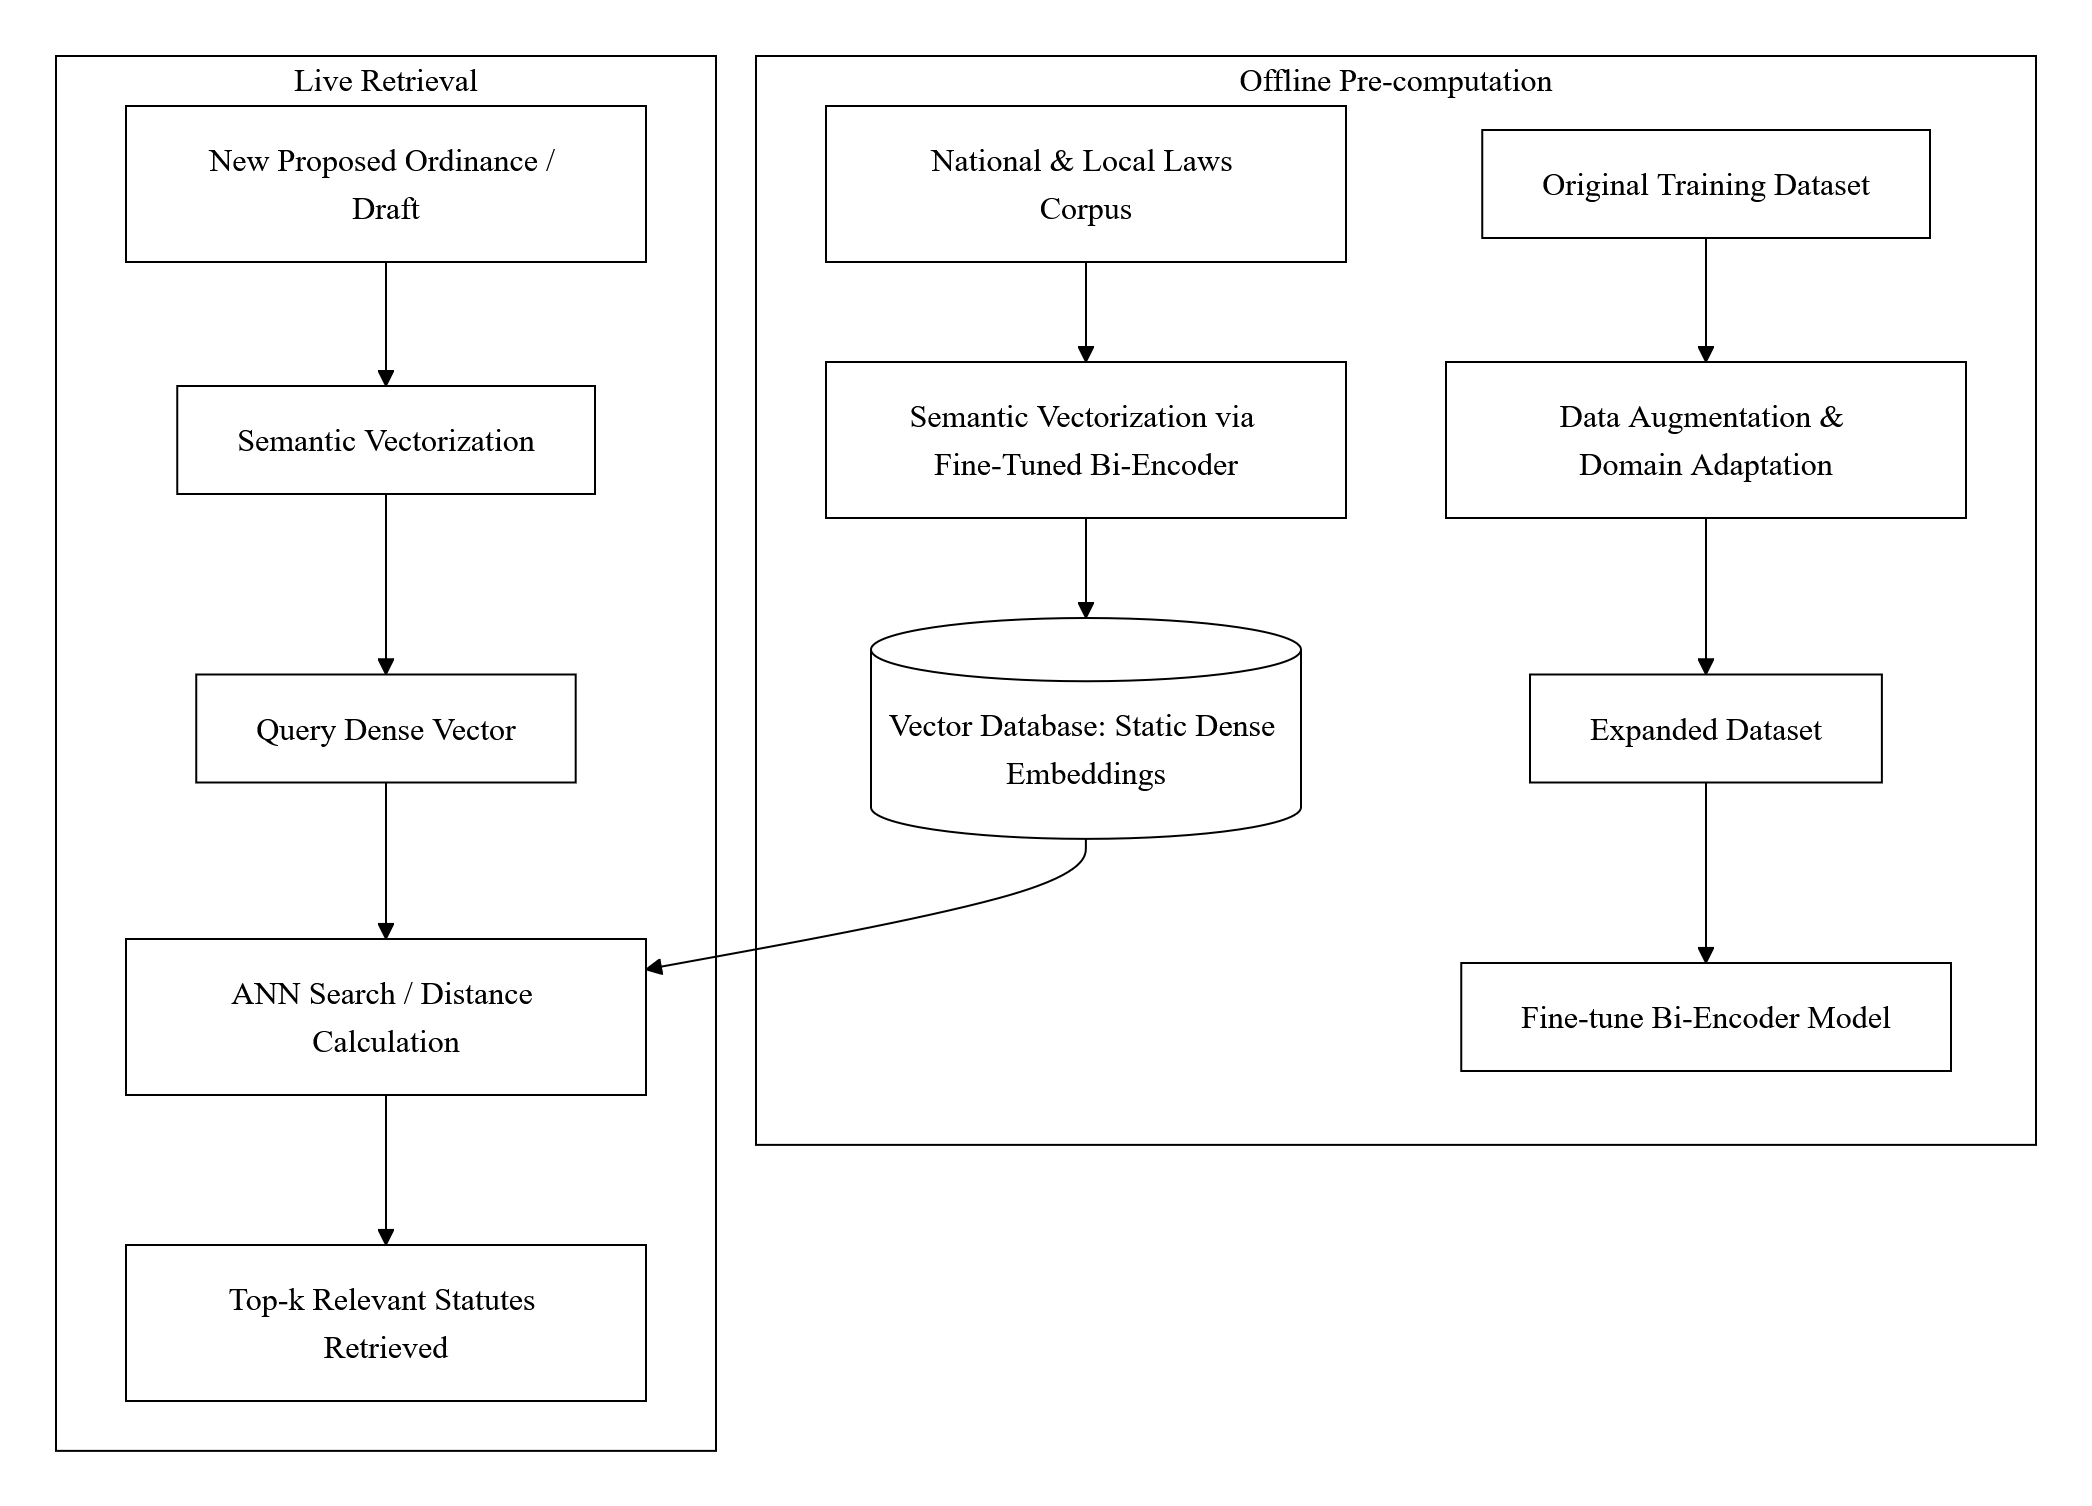
\includegraphics[width=1.0\linewidth]{figs/Phase_1_Retrieval_BW.png}
        \caption{Phase 1 - Statute Law Retrieval (Bi-Encoder Pipeline). Adapted from AIIR Lab's retrieval methodology.}
        \label{fig:phase1aiir}
    \end{figure}
    
        \begin{description}
            \item[Data Augmentation and Domain Adaptation.] By training on synthetically augmented legal datasets, dense retrieval models learn to recognize identical underlying statutory concepts regardless of whether they are expressed in archaic legal vocabulary or modern drafting syntax, substantially enhancing semantic robustness against lexical divergence.
            
            \item[Semantic Vectorization via Bi-Encoder.] The central component of Phase 1 is a Bi-Encoder architecture (such as \texttt{all-mpnet-base-v2}), which projects statutory text into a dense, continuous vector space. Unlike cross-encoders, which must process query-document pairs jointly and are computationally prohibitive across thousands of statutory enactments, bi-encoders encode queries and corpus documents independently. During contrastive fine-tuning, the embedding space is optimized such that vectors representing logically relevant statutory pairs exhibit high geometric proximity, while irrelevant pairs are separated under distance metrics such as cosine similarity.
            
            \item[Corpus Pre-computation and Vector Indexing.] To satisfy the operational requirement of querying tens of thousands of statutory documents efficiently, dense retrieval paradigms rely on offline pre-computation. Prior to query execution, the fine-tuned bi-encoder processes the statutory corpus, transforming individual statutory provisions into static, dense vector representations stored within an indexed vector database. Because corpus vectorization is decoupled from live query execution, dense retrieval scales effectively across extensive statutory archives without requiring real-time GPU re-encoding.
            
            \item[Live Query Vectorization and Proximity Scoring.] During query evaluation, the bi-encoder projects candidate draft provisions into the shared mathematical embedding space. Approximate nearest neighbor (ANN) search algorithms subsequently calculate geometric proximity (e.g., cosine similarity) between the query vector and pre-indexed statutory embeddings. Because this process computes continuous geometric distances rather than autoregressive tokens, high-throughput retrieval surfaces the top-$k$ most relevant statutory candidates in sub-second latency, providing high candidate recall to prime downstream natural language inference.
        \end{description}

    \subsection{Statute Law Retrieval by Team JNLP}
    Complementing pure bi-encoder retrieval, literature in computational law emphasizes multi-stage retrieval pipelines to balance candidate recall against ranking precision. Exemplified by Team JNLP's high-performing architecture in COLIEE benchmarks~\cite{coliee2025proceedings, goebel2026an}, this multi-stage paradigm progressively filters statutory search spaces across three structured phases: Pre-Retrieval Candidate Pruning, Model Fine-Tuning, and Result Ensembling.

    \begin{figure}[htbp]
        \centering
        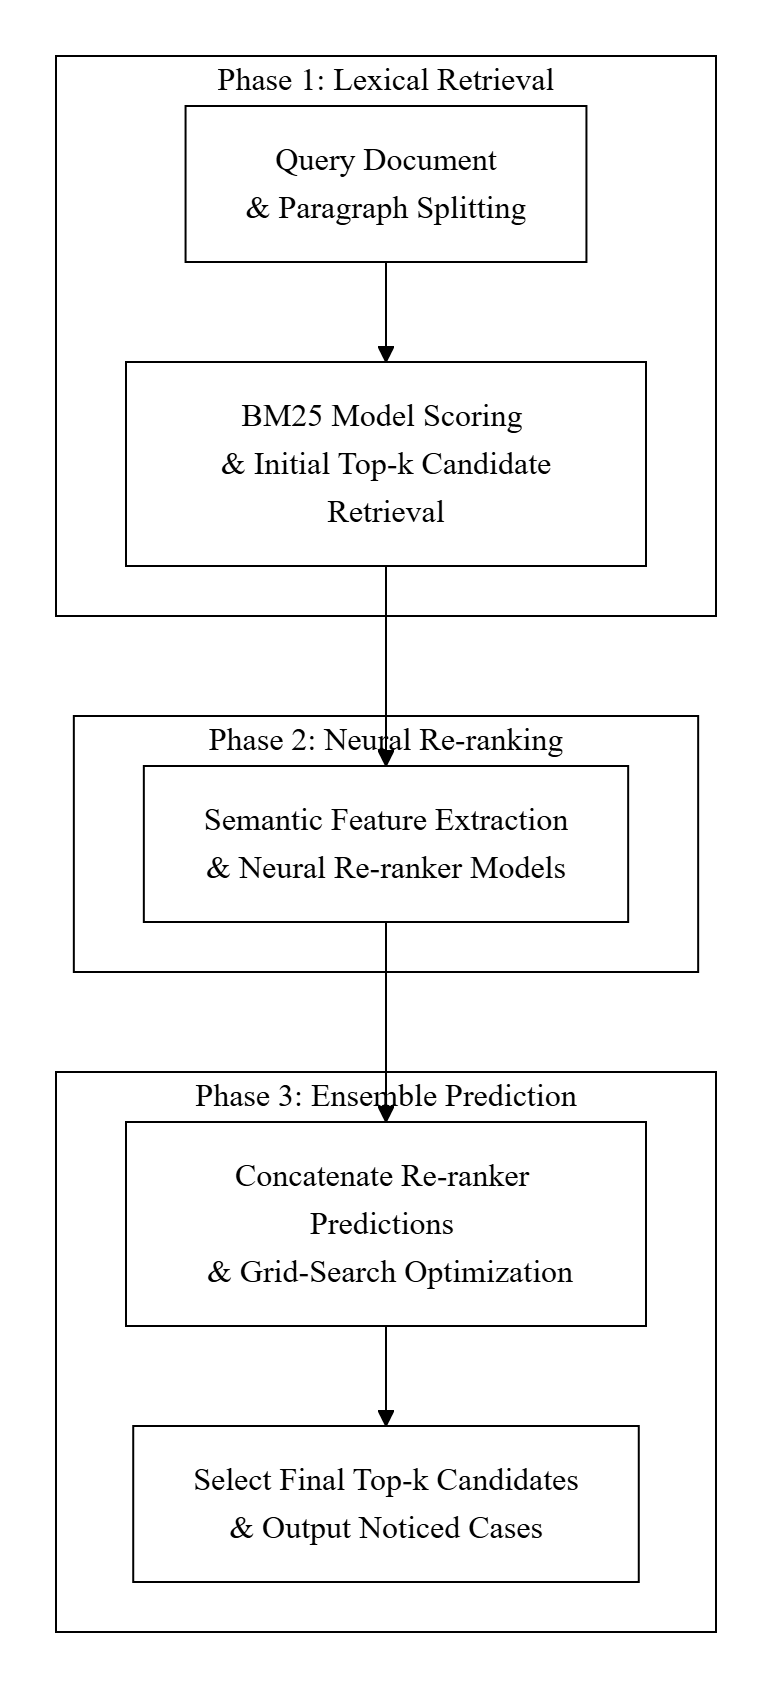
\includegraphics[width=0.6\linewidth]{figs/JNLP_Framework_BW.png}
        \caption{Phase 1 - Statute Law Retrieval (Bi-Encoder Pipeline). Adapted from JNLP's retrieval methodology.}
        \label{fig:phase1jnlp}
    \end{figure}

        \subsubsection{Pre-Retrieval}
        The primary objective of the initial phase is to drastically reduce the expansive search space while maintaining high recall across governing provisions, achieved through a multi-stage candidate pruning procedure.

            \begin{description}
                \item[Distance-Based Heuristic Filtering.] Dense embeddings for statutory queries and corpus provisions are extracted using high-capacity multilingual representations (e.g., BGE-M3). Rather than relying solely on raw cosine similarity, the methodology calculates multi-dimensional distance metrics (such as L1 distance bins), training a gradient-boosted decision tree to predict relevance and counter severe positive-negative sample imbalance.
                
                \item[Passage Re-ranking and Pruning.] The candidate pool is subsequently refined to eliminate non-relevant documents. A specialized neural passage re-ranker (such as RankLLaMA) evaluates candidate texts and prunes lower-ranked provisions, successfully narrowing the candidate set to top-ranked candidates while preserving recall.
            \end{description}

        \subsubsection{Model Fine-Tuning}
        Once the candidate space is constrained, the framework applies targeted natural language models to perform fine-grained relevance scoring.

            \begin{description}
                \item[Parameter-Efficient Model Adaptation.] Because fine-tuning large models across full parameter sets is computationally intensive, legal NLP frameworks leverage Parameter-Efficient Fine-Tuning (PEFT) techniques, such as LoRA and QLoRA. These techniques enable foundational language models to adapt to specialized statutory semantics with minimal memory overhead.
                
                \item[Class Imbalance Mitigation.] Because statutory candidate sets exhibit severe class imbalance (where only a small minority of retrieved provisions contain true preemption conflicts), sampling strategies and asymmetric loss functions are applied during training to preserve sensitivity to positive conflict signals.
            \end{description}

        \subsubsection{Result Ensemble}
        To maximize retrieval robustness and mitigate individual model variance, multi-stage retrieval pipelines aggregate relevance scores across distinct architectural paradigms.

            \begin{description}
                \item[Weighted Score Aggregation.] Rather than relying on uniform voting, relevance predictions are aggregated through weighted linear combinations of calibrated probabilities outputted by complementary lexical and neural models.

                \item[Hyperparameter Optimization.] The weighting coefficients assigned to individual scoring components are optimized via systematic hyperparameter search (e.g., Optuna), ensuring balanced contributions between lexical keyword precision and dense semantic recall.
            \end{description}

\subsection{Statute Law Textual Entailment by Team KIS}
    In the second phase of legal retrieve-then-entail architectures, the theoretical objective transitions from broad candidate discovery to fine-grained deontic reasoning. To ensure high computational throughput and deterministic classification, modern legal NLP frameworks deploy non-generative cross-encoder architectures, exemplified by the ModernBERT-based rationale extraction methodology developed by Team KIS~\cite{kadowaki2025modernbert}.

\begin{figure}[htbp]
    \centering
    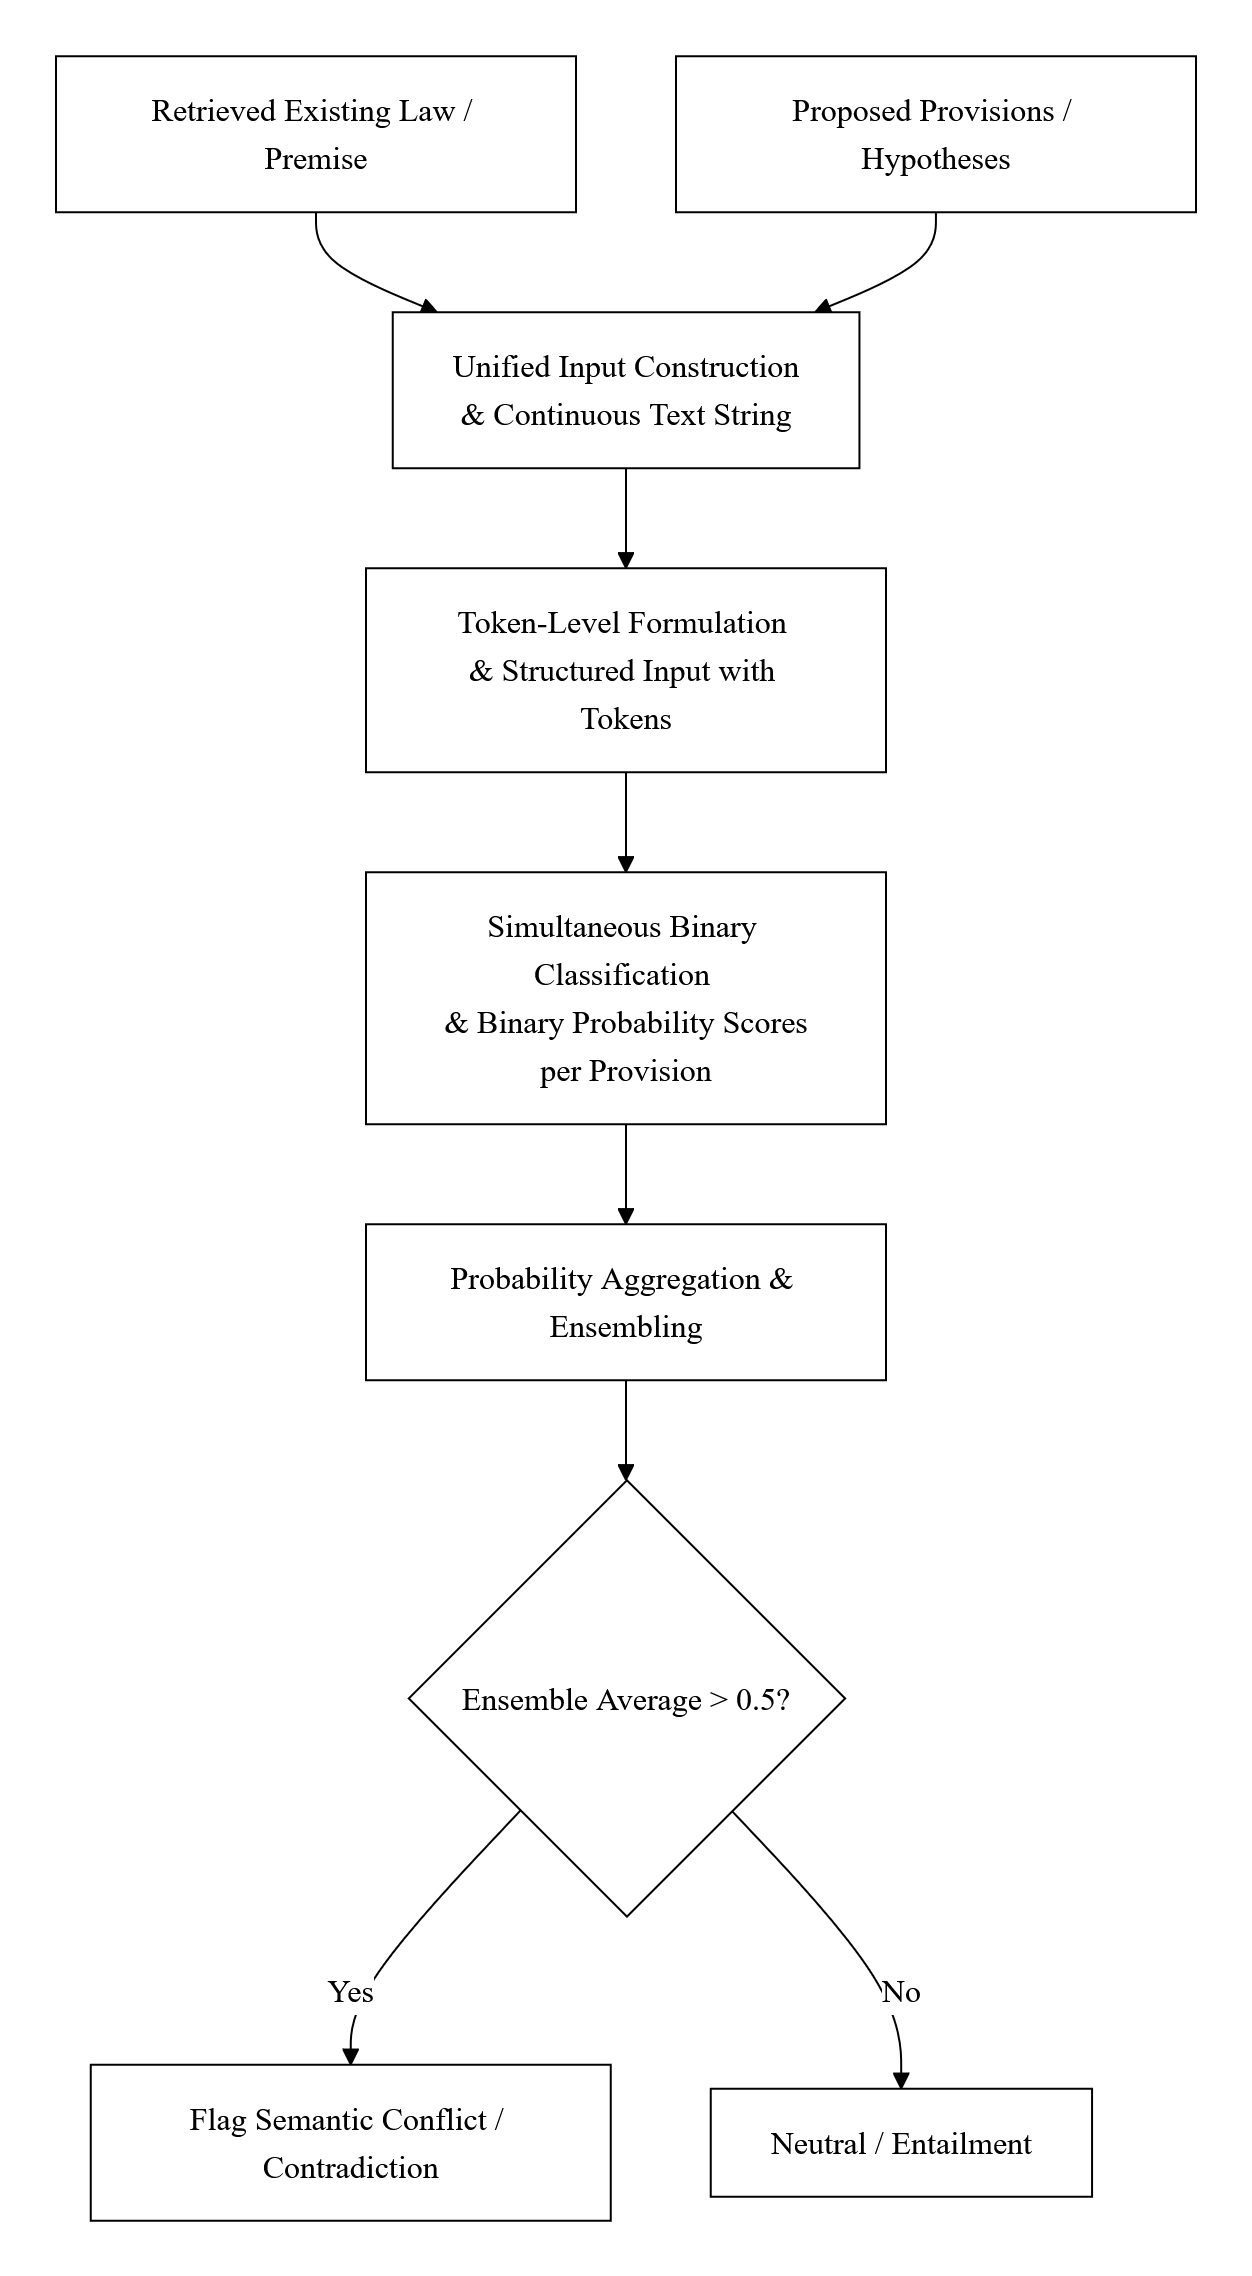
\includegraphics[width=0.7\linewidth]{figs/Phase_2_Entailment_BW.png}
    \caption{Phase 2 - Statutory Textual Entailment (NLI Pipeline). Adapted from Team KIS's ModernBERT rationale extraction methodology.}
    \label{fig:phase2}
\end{figure}
    
    This entailment framework is structured around four theoretical components:

    \begin{description}
        \item[Unified Input Construction.] While traditional transformer encoders are constrained by short sequence limits (e.g., 512 tokens), requiring aggressive document truncation, modern architectural designs support extended context windows up to 8,192 tokens. Under this formulation, retrieved statutory context (the premise) and candidate draft provisions (the hypothesis) are concatenated into a unified sequence. Strategic token boundaries clearly demarcate statutory premises from draft hypotheses.
        
        \item[Token-Level Problem Formulation.] To evaluate targeted normative conflicts within candidate provisions, the framework structures input sequences with dedicated segment tokens (e.g., \texttt{<sep>}). This formats multi-clause statutory text into an aligned representation suitable for direct cross-attention.
        
        \item[Simultaneous Multi-Target Classification.] The unified sequence is processed by an efficient bidirectional encoder. Because the architecture operates purely as a sequence classifier, it eliminates the computational latency and hallucination vulnerabilities inherent in autoregressive text generation. Instead, the model evaluates segment separation tokens to generate class probabilities, determining whether candidate provisions logically entail, contradict, or remain neutral relative to governing law.
        
        \item[Probability Calibration and Ensembling.] To maximize predictive reliability and mitigate single-model bias, the framework incorporates probability aggregation across diverse model checkpoints or hyperparameter variations. Averaged or calibrated posterior probabilities exceeding decision thresholds indicate detected normative conflict with formal statistical backing.
    \end{description}

\subsection{Theoretical Synthesis}
This synthesis integrates the foundational theoretical models reviewed throughout this chapter into a unified paradigm for ex-ante legislative conflict detection. While each individual methodology addresses an isolated phase of legal document processing, their conceptual integration establishes a principled retrieve-then-entail framework:

\begin{description}
    \item[Dense Retrieval Methodology.]
    The theoretical foundation for statutory candidate discovery draws from the dense retrieval methodology established by the \textbf{AIIR Lab}~\cite{wu2025aiir, largey2026aiirlab}. Their approach demonstrates that targeted domain augmentation mitigates OCR noise in archival legal text, while continuous semantic vectorization enables high-throughput candidate identification across large statutory collections without relying on rigid keyword indices.

    \item[Ensemble Learning Strategy.]
    To balance candidate recall against precision, the framework incorporates the multi-stage ranking principles demonstrated by \textbf{Team JNLP}~\cite{coliee2025proceedings, goebel2026an}. This methodology utilizes lexical filtering (BM25) to prune extraneous documents, followed by neural scoring and rank fusion to isolate authoritative candidate enactments on standard computing hardware.

    \item[Textual Entailment.]
    For granular deontic conflict evaluation, the framework adopts the \textbf{Team KIS framework} for textual entailment~\cite{kadowaki2025modernbert}. Their methodology formats premise-hypothesis pairs into a continuous sequence evaluated via lightweight cross-encoders, utilizing token-level separation boundaries to classify logical relationships without generative hallucination risks.

    \item[Synthesis and Benchmark Consensus.]
    Synthesizing these foundational frameworks establishes an end-to-end theoretical foundation for automated preemption auditing. The retrieval stage narrows extensive statutory search spaces down to high-probability candidate provisions, while the textual entailment stage conducts deterministic normative conflict checks. The latest findings from the COLIEE 2026 proceedings~\cite{coliee2026proceedings, ngo2026nowj} reinforce this architectural consensus, validating that pipelined retrieval and textual entailment provide the most reliable foundation for automated legal consistency analysis.
\end{description}

%\section{Theoretical Framework}
The evolution of legal information processing has necessitated a transition from traditional keyword-based retrieval toward sophisticated, multi-stage frameworks that are capable of handling the logical nuances and the so-called "legalese" of legislative text.

In the context of the Philippine unitary state, preserving the legal hierarchy requires a robust mechanism to ensure that local ordinances do not contravene national statutes. As research specifically targeting automated consistency checking in Philippine local archives remains scarce, the proposed theoretical framework establishes its foundation by adapting the empirical methodologies of the Competition on Legal Information Extraction and Entailment (COLIEE). 

While COLIEE traditionally focuses on retrieving statutes to answer bar exam questions, this study repurposes its "Retrieve-Then-Entail" paradigm to operationalize jurisprudential doctrine within an automated system. This framework is structured around three primary pillars: (1) The Jurisprudential Constraint, (2) The Operational Framework, and (3) The Interpretive Mechanism. By integrating the multi-stage strategies demonstrated in the COLIEE paradigm, the system provides a specialized foundation for the novel task of automated semantic conflict detection between Republic Acts and local ordinances. \cite{nguyen2025nowjcoliee2025multistageframework}.

This framework is structured around three primary pillars: (1) The Jurisprudential Constraint, (2) The Operational Framework, and (3) The Interpretive Mechanism. By integrating the multi-stage paradigms and large language model (LLM) reasoning strategies demonstrated in recent COLIEE competitions, the system provides a comprehensive foundation for automated semantic conflict detection.\cite{nguyen2025nowjcoliee2025multistageframework}.

\subsection{The COLIEE Paradigm as a Methodological Foundation}
The Competition on Legal Information Extraction (COLIEE) provides the empirical and methodological foundation for the proposed system. As an annual evaluation contest, COLIEE benchmarks the state-of-the-art in legal case retrieval, statute law entailment, and legal question answering. By adopting the COLIEE framework, the system moves beyond simple keyword matching and integrates advanced techniques, which include domain-adapted pre-training, transformer-based neural methods, and hybrid ensemble architectures.

    \subsubsection{Task Taxonomy and Legislative Relevance}
    The COLIEE competition includes specific tasks targeting statute law processing. These tasks align with the requirements of the Philippine legislative environment, particularly when it comes to handling the transition from broad retrieval of the Republic Acts to fine-grained logical analysis of local ordinances. From the COLIEE competition, the following tasks were found relevant to this study:

    \begin{description}
        \item[Task 3: Statutory Law Retrieval:] This task requires retrieving relevant articles from a statutory corpus (such as the Japanese Civil Code or, in this context, the collection of Philippine Republic Acts) that support or relate to a given legal query. This is the direct equivalent of finding the specific national laws that a local ordinance might be attempting to modify or contradict.
        
        \item[Task 4: Statute Law Entailment:] This involves determining if a retrieved set of statutes semantically entails a specific legal conclusion, usually framed as a "Yes" or "No" answer to a query. In this framework, Task 4 is the computational realization of the "No Contravention" test from the Magtajas Doctrine, determining whether the local ordinance (Hypothesis) is logically consistent with the retrieved national law (Premise).
    \end{description}
    
    The "Retrieve-Then-Entail" paradigm, where Task 3 serves as a preliminary stage for Task 4, is essential for managing the extremely long document contexts inherent in legislative data. This sequential approach ensures that the more computationally expensive entailment models are only applied to a refined set of relevant statutes, balancing efficiency and accuracy.

\subsection{Pillar 1: The Jurisprudential Constraint (Magtajas-NLI Mapping)}

The foundational logic of this study rests on the Unitary Principle of the State, which dictates that local government units (LGUs) exercise only delegated legislative powers \cite{philgov1991ra7160}. In the Philippine legal hierarchy, the 1987 Constitution is the supreme law, followed by national statutes, while local ordinances occupy the lowest rung \cite{philgov1991ra7160} Consequently, no local ordinance may validly ignore, contradict, or refuse to implement an Act of Congress.
To operationalize this hierarchy for an automated system, the framework utilizes the Magtajas Doctrine, which establishes six substantive requirements for the validity of a municipal ordinance (source) \cite{scp1994magtajasvpryce}. This study maps these legal requirements directly onto the task of Natural Language Inference (NLI), where the national law serves as the Premise $P$ and the proposed ordinance serves as the Hypothesis $H$.

%NLI-Mapping Table
\noindent
\begin{tabularx}{1\textwidth} { 
    @{}
  | >{\raggedright\arraybackslash}X 
  | >{\raggedright\arraybackslash}X 
  | >{\raggedright\arraybackslash}X | 
  @{}}
 \hline
 \textbf{Magtajas Requirement}
 & \textbf{Legal Constraint}
 & \textbf{NLI Task Mapping} \\
 \hline
 \textbf{No Contravention}  
 & Must not contradict national statutes.  
 &\textbf{Contradiction Detection: }Determining if $P$ and $H$ are logically incompatible.  \\
\hline
\textbf{Non-Discriminatory}
&Must not be partial or discriminatory.
&\textbf{Bias and Entity Recognition:} Identifying protected groups or classes.\\
\hline
\textbf{Trade Regulation}
& Must not prohibit, but may regulate trade.
&\textbf{Deontic Logic Analysis:} Distinguishing between absolute prohibitions and conditional permissions. \\
\hline
\textbf{Public Policy Alignment}
& Must be consistent with public policy.
&\textbf{Semantic Entailment:} Assessing if the ordinance aligns with the broader intent of the law. \\
\hline
\end{tabularx}

The requirement that an ordinance must not contravene a statute is the most critical for automated systems. As noted in the Magtajas ruling, local councils exercise only delegated powers; thus, the delegate cannot be superior to the principal \cite{scp1994magtajasvpryce}. This necessitates a system that can effectively perform "Statute Law Retrieval" (finding the relevant national law) and "Statute Law Entailment" (verifying the logical compatibility), which are the core focuses of Tasks 3 and 4 in the COLIEE competition.



\subsection{Pillar 2: The Operational Framework (Coarse-to-Fine Pipeline)}
To handle the legislative data in this study, the framework adapts the multi-stage architecture proven successful in the COLIEE paradigm for processing large-scale statutory corpora. This decoupled pipeline is influenced by top-performing methodologies such as ViDRILL (2025) and NOWJ (2025), tailored to bridge the "Semantic Gap" between literal keywords and normative intent within the Philippine LGU context.

\begin{enumerate}
    \item \textbf{Stage 1: Data Pre-processing and Context Compression:} Statutory documents typically exceed the input limits of standard pre-trained language models. Furthermore, these documents often contain noise such as procedural metadata and formatting errors.
    \begin{description}
            \item[Noise Reduction:] The system performs pre-processing by filtering out metadata, such as procedural details, locations, and irrelevant language fragments, ensuring that only the legally relevant content remains.

            \item[Abstractive Summarization:] To enhance the representation of long legislative documents, the framework employs LLM-based summarization. Following the ViDRILL (2025) multi-stage framework, the system utilizes a dual-level chunking strategy optimized for retrieval and re-ranking to ensure semantic robustness in long and structured texts. \cite{goebeletal2026coliee2025}
    \end{description}
    
    \item \textbf{Stage 2: Coarse Phase (Long-Context Retrieval):} The retrieval phase utilizes a dual approach of lexical and semantic matching to ensure high recall of relevant national statutes.
    \begin{description}
        \item[Pre-ranking Model:] The system employs a pre-trained bi-encoder, such as BGE-m3, to calculate initial relevance scores between the ordinance and candidate statutes. BGE-m3 is selected for its ability to process sequences of up to 8,192 tokens without destroying the structural integrity of the text.

        \item[Re-ranking with Cross-Encoders:] Once candidates are isolated, the system applies more granular ranking models. Following the NOWJ methodology, the system utilizes LLM2Vec, which enables bi-directional attention and unsupervised contrastive learning for text encoding.

        \item[LLM2Vec Integration:] Following the NOWJ methodology, the system utilizes LLM2Vec, which enables bi-directional attention and unsupervised contrastive learning for text encoding. 
    \end{description}
    
    \item \textbf{Stage 3: Fine Phase (Natural Language Inference and Reasoned Entailment):} In the final stage, the system performs the logical check for conflict. While the COLIEE paradigm traditionally utilizes NLI to verify if statutes support a legal conclusion, this framework repurposes that NLI logic to identify conflicting relations (contradictions).

    \begin{description}
        \item[Dual-Encoder Inference:] Adopting the TSRCDF-SS (2024) framework for legal conflict detection, the system employs independent encoders (e.g., SBERT and SimCSE) to vectorize and concatenate requirement sentence pairs \cite{wang2025transferlearningapproachautomatic}. Unlike retrieval, which measures topical similarity, this adapted NLI detects the logical incompatibility (e.g., a "prohibition" in an ordinance contradicting a "permission" in a Republic Act) that exists beneath shared syntax. \cite{kimetal2024legalinformationretrieval}
        
        \item[LLM-Based Analysis]:  The system prompts state-of-the-art LLMs such as DeepSeek-V3 or QwQ-32B for the final entailment judgment.  To improve reliability, the framework employs majority voting across multiple LLMs. A conflict is only confirmed if there is a consensus among distinct models, significantly boosting precision in the final detection results. \cite{goebeletal2026coliee2025}

        \item[Explainability:] To provide a verifiable ratio decidendi, the system extracts Attention Weights from the transformer layers to generate heatmaps that highlight the specific conflicting phrases—such as where an ordinance's "absolute ban" contradicts a statute's "conditional permit."
    \end{description}
\end{enumerate}

\subsection{Pillar 3: The Interpretive Mechanism (Computational Hermeneutics)}
The framework mathematically operationalizes the Hermeneutic Circle—the principle that a part of a text is understood in relation to the whole, and the whole in relation to its parts \cite{Kommers2026Hermeneutics}. This mechanism is realized through the Transformer’s self-attention mechanism, which allows every word in a provision to be weighted against every other word in the context window\cite{Guenmayor2018CaseStudyHermeneutics}. 

In legal interpretation, the canon of noscitur a sociis dictates that a word is known by the company it keeps. In Magtajas v. Pryce, the Supreme Court applied this rule to determine that the phrase "gambling and other prohibited games of chance" referred only to illegal gambling because of its surrounding context. The self-attention mechanism computationally replicates this by calculating the interaction of Query ($Q$), Key ($K$), and Value ($V$) matrices:

$$Attention(Q, K, V) = \text{softmax}\left(\frac{QK^T}{\sqrt{d_k}}\right)V$$

This allows the model to resolve Contextual Polysemy—where common words like "party" or "consideration" assume specialized meanings based on surrounding "legalese"—by dynamically adjusting vector representations based on the local syntactic context.

\subsection{Synthesis of Empirical Performance from COLIEE 2025}

\subsubsection{Performance Metrics for Statute Law Retrieval (Task 3)}
For Task 3, ensemble strategies centered on linear combinations of scores from top-performing base models (such as NV-Embed and e5-large) provided the most reliable results.

\noindent
\begin{tabularx}{1\textwidth} { 
    @{}
  | >{\raggedright\arraybackslash}X 
  | >{\raggedright\arraybackslash}X 
  | >{\raggedright\arraybackslash}X
  | >{\raggedright\arraybackslash}X | 
  @{}}
 \hline
 \textbf{Team Strategy}
 & \textbf{F2 Score}
 & \textbf{Precision}
 & \textbf{Recall} \\
 \hline
 \textbf{NOWJ.H2 (Grid Search)}  
 & 0.7702  
 & 0.7572
 & 0.8086 \\
\hline
\textbf{NOWJ.H1 (LightGBM)}
&0.7311
&0.7352
&0.7511\\
\hline
\textbf{NOWJ.H3 (Similarity Voting)}
&0.7069
&0.7534
&0.7100\\
\hline
\end{tabularx}

The efficacy of the Grid Search weighted ensemble suggests that meticulous optimization of high-quality input signals is pivotal for success, particularly in achieving high recall—a critical requirement for ensuring no relevant national statute is missed.

\subsubsection{Performance Metrics for Statute Law Entailment (Task 4)}
In the entailment task, state-of-the-art results were achieved using LLMs coupled with advanced prompt engineering.

\noindent
\begin{tabularx}{1\textwidth} { 
    @{}
  | >{\raggedright\arraybackslash}X 
  | >{\raggedright\arraybackslash}X | 
  @{}}
 \hline
 \textbf{Team}
 & \textbf{Accuracy} \\
 \hline
 \textbf{KIS3}  
 & 0.9041 \\
\hline
\textbf{CAPTAIN2}
&0.8219\\
\hline
\textbf{JNLP002}
&0.8082\\
\hline
\textbf{NOWJ (Various Runs)}
&0.7397\\
\hline
\end{tabularx}


The high accuracy scores (up to 0.9041) validate the potential of LLMs to handle complex legal reasoning and provide reliable "Yes/No" answers regarding whether a given statute entails the query. For the Philippine system, this demonstrates that a similar architecture can reliably detect whether an ordinance's provisions are semantically consistent with a Republic Act.

\subsection{Theoretical Integration: Bridging Doctrine with Pipeline}
\noindent
\begin{tabularx}{1\textwidth} { 
    @{}
  | >{\raggedright\arraybackslash}X 
  | >{\raggedright\arraybackslash}X 
  | >{\raggedright\arraybackslash}X | 
  @{}}
 \hline
 \textbf{Legal Pillar}
 & \textbf{Mechanism}
 & \textbf{Computational Realization} \\
 \hline
 \textbf{Jurisprudential}  
 & Magtajas Doctrine
 & NLI Task Mapping ($P$ as Statute, $H$ as Ordinance).\\
\hline
\textbf{Operational}
& Coarse-to-Fine Pipeline
& Task 3 (Retrieval) and Task 4 (Entailment) using LLMs and Ensembles.\\
\hline
\textbf{Interpretive}
& Context Machine
& Transformer Self-Attention ($Q, K, V$) and the Hermeneutic Circle.\\
\hline
\end{tabularx}

By grounding the system in the COLIEE statutory tasks, the framework addresses the "long text problem" through abstractive summarization and ensures that the system remains explainable and calibrated. This approach equips the system to handle the complexities of legal language in a unitary state, ensuring that the delegate (the LGU) remains consistent with the principal (the National Legislature).
\begin{figure}[htbp]
    \centering
    % Adjust width=1\textwidth
    \includegraphics[width=1\textwidth]{CS_Undergraduate_Thesis_Template/figs/[UPDATED] Theoretical Framework (Thesis).png}
    \caption{Integrated Theoretical Framework for Semantic Conflict Detection in Philippine Local Legislation.}
    \label{fig:theoretical_framework}
\end{figure}


% !TeX root = ../main.tex

\chapter{Methodology}
This chapter explains the methodology used to build and evaluate the Coarse-to-Fine Semantic Conflict Detection System. It describes how Philippine legal texts are collected and cleaned, and how the two-stage Retrieve-then-Entail architecture is organized. The chapter also details the creation of the ground truth dataset and the selection of candidate models. Finally, it outlines the evaluation metrics and hardware constraints, which are chosen to match the computing capacity of an average Local Government Unit (LGU).


\section{Conceptual Framework}
This section maps how data flows through the proposed system. The architecture follows an Input-Process-Output (IPO) design organized into a two-stage ``Coarse-to-Fine'' retrieve-then-entail pipeline (Figure~\ref{fig:conceptualframework}). By decoupling broad statutory candidate retrieval from compute-intensive textual entailment classification, the framework overcomes the combinatorial explosion and hardware bottlenecks that traditionally impede local legal NLP deployment. The workflow is divided into two operational phases: Phase~1 (Offline Foundation and Optimization) and Phase~2 (Live Online Retrieve-then-Entail Pipeline).

    \begin{figure}[htbp]
        \centering
        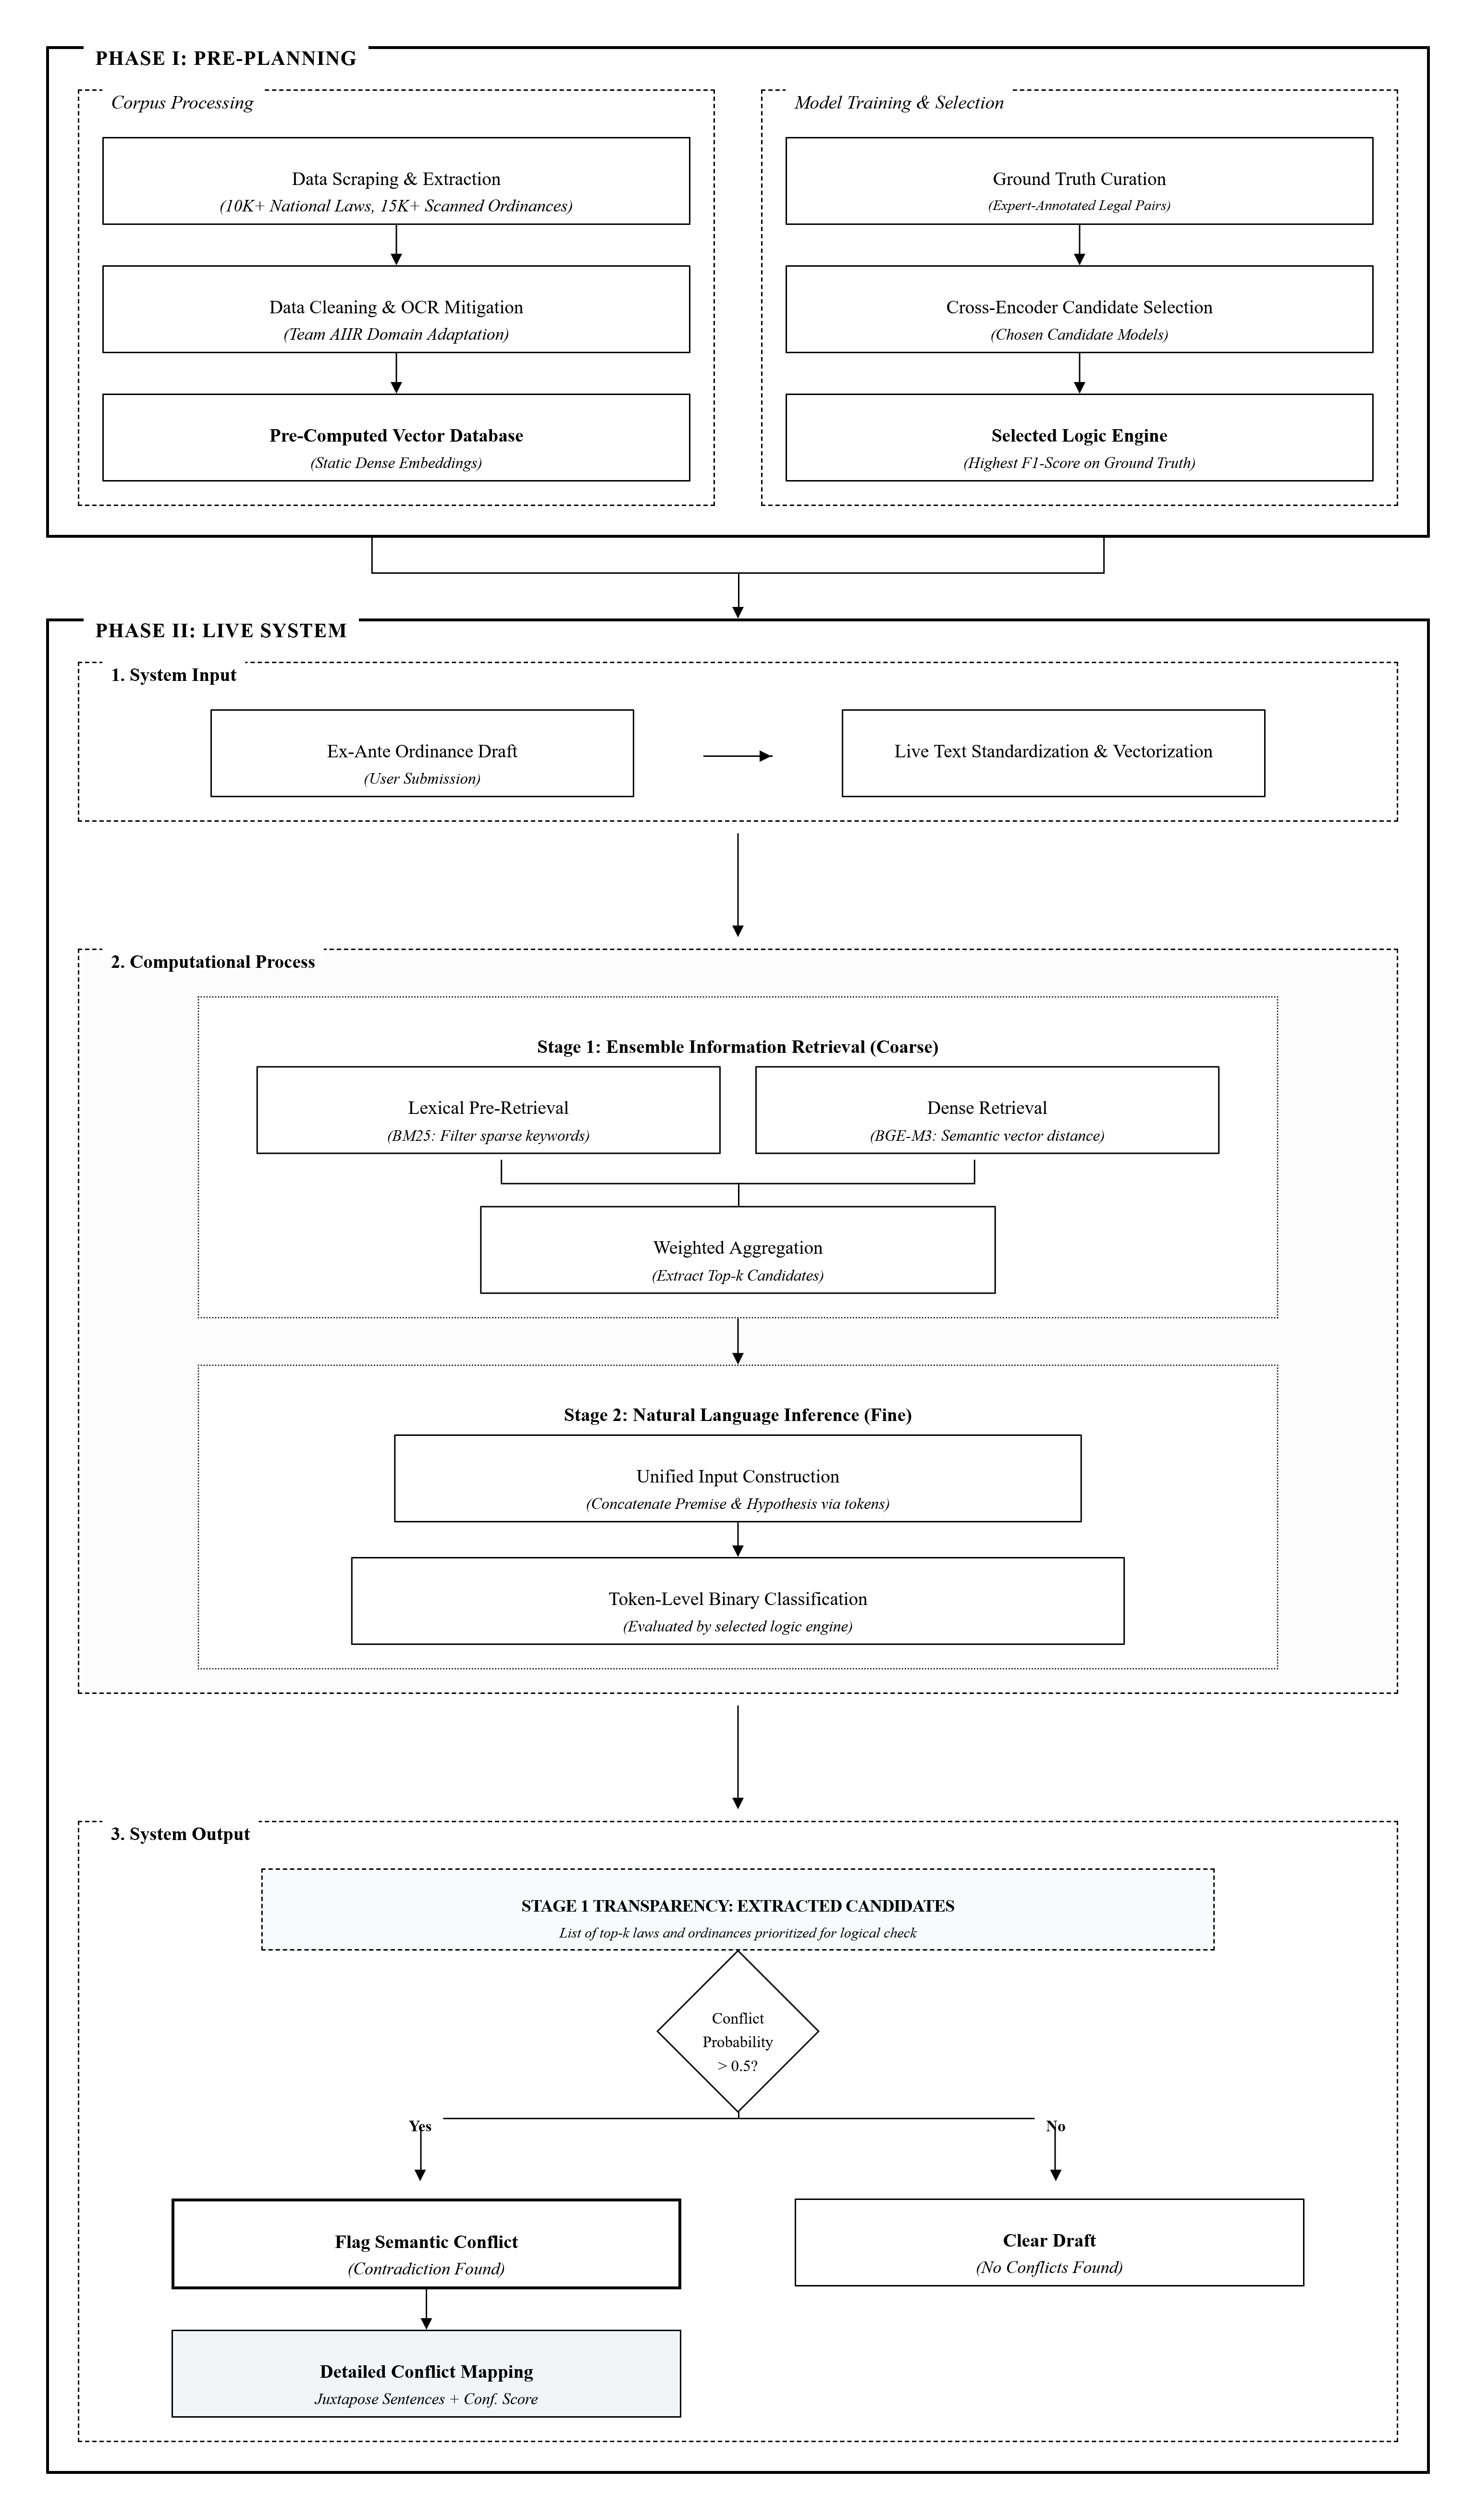
\includegraphics[width=0.88\linewidth]{figs/conceptual_framework_flowchart.png}
        \caption{Detailed Information Flow of the Coarse-to-Fine Semantic Conflict Detection Architecture.}
        \label{fig:conceptualframework}
    \end{figure}

    \subsection{Phase 1: Pre-Planning (Offline Foundation \& Optimization Protocol)}
    This preliminary phase establishes the empirical foundation of the system by compiling the statutory corpus, building pre-computed retrieval indexes, and selecting the optimal transformer logic engines through a structured benchmark screening protocol.

    \begin{description}
        \item[Dual-Corpus Ingestion \& Pre-Computation Protocol.] The system compiles a comprehensive dual-jurisdiction statutory archive combining the Philippine national statutory collection (Republic Acts, Executive Orders, Presidential Decrees, Acts, Batas Pambansa, and Commonwealth Acts) with Davao City municipal legislation (historical Landmark Ordinances and digital LISSP municipal records). The compiled corpus undergoes legal text normalization, optical character recognition (OCR) noise mitigation on historical scans, and structural section segmentation into granular, self-contained regulatory units ($\sim 200\text{--}300$ tokens). Cleaned statutory provisions are then indexed offline: dense semantic representations are pre-computed using a lightweight transformer bi-encoder, while sparse inverted lexical indexes are constructed using BM25 ($k_1 = 1.5, b = 0.75$) alongside unsupervised statutory topic modeling.
        
        \item[Model Benchmark \& Selection Protocol.] Candidate architectures are screened and fine-tuned against a curated Ground Truth Legal Benchmark stratified across three granular difficulty tiers: Tier~1 (Surface Lexical), Tier~2 (Structural Preemption), and Tier~3 (Latent Semantic). A multi-stage empirical screening and ablation protocol evaluates candidate bi-encoders (balancing inference latency against candidate Recall@$k$) and candidate cross-encoders (evaluating precision, latency, and quantization trade-offs across FP32, FP16, and INT8 axes). Based on these empirical evaluations, the highest-performing models are selected as the production engines: an optimal dense bi-encoder for Stage~1 candidate retrieval, and an optimal fine-tuned cross-encoder for Stage~2 contradiction reasoning.
    \end{description}

    \subsection{Phase 2: Live System (Online Retrieve-then-Entail Pipeline)}
    The live system executes the automated conflict detection pipeline when a newly drafted municipal measure is submitted for pre-enactment review, operating through an Input-Process-Output structure.

    \begin{description}
        \item[1. System Input.] A legislative researcher uploads a newly proposed ex-ante ordinance draft. Because draft measures originate within local government offices as digital-born documents (.docx or digital PDF), they are free from optical scanning noise. The ingestion pipeline segments the draft into individual substantive provisions, filtering out non-regulatory procedural boilerplate (such as the Title, Separability, Repealing, and Effectivity clauses). The isolated substantive provisions are vectorized in real time via the selected dense bi-encoder alongside sparse lexical token extraction.
        
        \item[2. Computational Process.] The computational core executes two complementary stages:
            \begin{description}
                \item[Stage 1: Dual-Stream Hybrid Information Retrieval.] The system narrows the comprehensive statutory search space down to a focused candidate pool. Stream~A executes lexical sparse search via BM25 to match exact statutory citations, numerical penalty amounts, and administrative agency terms. Stream~B executes dense semantic search via the selected bi-encoder, measuring cosine similarity between the draft provision and statutory embeddings to capture abstract regulatory intent. The ranked outputs are combined using Reciprocal Rank Fusion (RRF) integrated with a Statutory Hierarchy Safeguard (prioritizing higher-ranking national statutes over municipal provisions). This hybrid coarse filter extracts the Top-$k$ candidate provisions without overburdening local LGU compute resources.

                \item[Stage 2: Natural Language Inference.] Each retrieved statutory candidate is paired with the draft ordinance provision into a single cross-encoder sequence:
                \[
                    \mathbf{x} = [\text{CLS}] \; \text{Retrieved Statutory Premise} \; [\text{SEP}] \; \text{Proposed Ordinance Clause} \; [\text{SEP}]
                \]
                The unified sequence is processed by the selected fine-tuned cross-encoder NLI engine, which performs full inter-token cross-attention to classify the directional logical relationship (entailment, neutral, or contradiction) and produce a calibrated contradiction probability $P(\text{Contradiction})$.
            \end{description}

        \item[3. System Output \& Explainable Reporting.] The system presents an audit trail displaying the Top-$k$ shortlisted candidate statutes for human oversight before evaluating contradiction probability against a calibrated decision threshold $\tau^*$ (optimized for recall priority via $F_2$-score weighting):
            \begin{itemize}
                \item \textbf{Flag Semantic Conflict ($P(\text{Contradiction}) \ge \tau^*$):} The system flags a normative legal inconsistency and routes it through a Two-Tiered Jurisdictional Conflict Classification:
                \begin{enumerate}
                    \item \textit{Critical Vertical Preemption Alert:} Flags collisions with superior national statutes under the \textit{Magtajas} doctrine and RA~7160 \S5(a) (e.g., an ordinance permitting what a national statute forbids).
                    \item \textit{Horizontal Inconsistency Notice:} Flags collisions or uncoordinated overlaps with prior Davao City municipal ordinances, signaling necessary amendments or harmonization.
                \end{enumerate}
                To provide transparency, the system renders Intrinsic Structural Explainability (XAI) featuring side-by-side comparative spans, highlighted conflicting phrases, and calibrated confidence percentages.

                \item \textbf{Clear Draft Measure ($P(\text{Contradiction}) < \tau^*$):} If no normative contradictions exceed the calibrated decision threshold, the system issues a formal legislative compliance confirmation, accompanied by a Statutory Clearance and Traceability Audit confirming both national statutory harmony and local municipal code coherence.
            \end{itemize}
    \end{description}


\section{Research Design and Implementation}
This section outlines the methodology for data collection, system engineering, and evaluation. It explains the protocols used to build the pipeline from raw text gathering to the final prototype demonstration.

\subsection{Research Design}
    This study uses an applied research design to build a practical software tool for local governance. The researchers use an experimental systems development approach to solve the delays and difficulties of manual ordinance review through automated detection. This setup connects principles from legal informatics and natural language processing to address a real local need. By focusing on practical transformer-based models, the design connects theoretical computer science with everyday government office work. The experiment directly tests whether a retrieve-then-entail pipeline can operate reliably in a local legislative setting.

    The experimental setup tests the retrieval and classification modules separately to measure search speed and accuracy independently. Building the system step-by-step allows the researchers to adjust the information retrieval and natural language inference stages using local legal texts. This engineering process ensures that the finished tool accounts for the writing styles found in both city ordinances and national statutes. In this way, applied research methods help turn modern NLP concepts into a usable tool for the Davao City Sangguniang Panlungsod. As a result, the findings establish a clear benchmark for automating pre-enactment legal checks on local legislation.

    \subsection{Corpus Acquisition}
    \label{sec:corpus_acquisition}
    Building the legal database requires collecting text from different public repositories so that the system includes as many relevant laws as possible. These sources provide the national statutes and city ordinances needed to check draft legislation for consistency. To keep the language consistent and make vector processing simpler, the system gathers only the English-language versions of all legal texts. This choice matches Philippine statutory rules under Section~20, Chapter~5, Book~I of Executive Order No.~292 (Administrative Code of 1987)~\cite{philgov1987eo292}, which explicitly mandates that in the interpretation of laws promulgated in official languages, the English text shall control unless otherwise specifically provided. National statutes and local ordinances are gathered using separate automated scripts designed for the format of each source.

        \subsubsection{Corpus Composition}
        The Lawphil Project (Arellano Law Foundation) serves as the primary digitized extraction source for national statutory text because its documents are provided in clean HTML, follow a consistent layout, and offer broad historical coverage~\cite{lawphil2000}. Automated scraping scripts browse through chronological and alphabetical indexes to collect Republic Acts, Batas Pambansa, Commonwealth Acts, Acts, Executive Orders, and Presidential Decrees. Using a custom web extraction pipeline built by the proponents, statutory extraction was conducted as of \textbf{March 2026}, collecting 25,432 unique legal records enacted between 1900 and 2026. The Official Gazette of the Republic of the Philippines~\cite{officialgazette} and the Chan Robles Virtual Law Library were used as authoritative secondary cross-references to verify enactment dates, chronological numbering, and historical amendment status. All collected national laws are converted into standardized JSON records with metadata, such as dates of approval, titles, and section numbers. Listing~\ref{lst:corpus_extraction} illustrates the web scraping and provision extraction logic implemented to retrieve and structure the statutory archive. As illustrated in Figure~\ref{fig:lawphil_web_interface}, the Lawphil repository presents statutory text in clean, unstyled HTML typography with a predictable hierarchical URL schema (e.g., \texttt{/statutes/repacts/ra2018/ra\_11035\_2018.html} for Republic Act No.~11035). This standardized structure separates introductory legislative headers from operative provisions and eliminates the need for dynamic JavaScript browser rendering, facilitating rapid, fault-tolerant web scraping.

        \begin{figure}[!htbp]
            \centering
            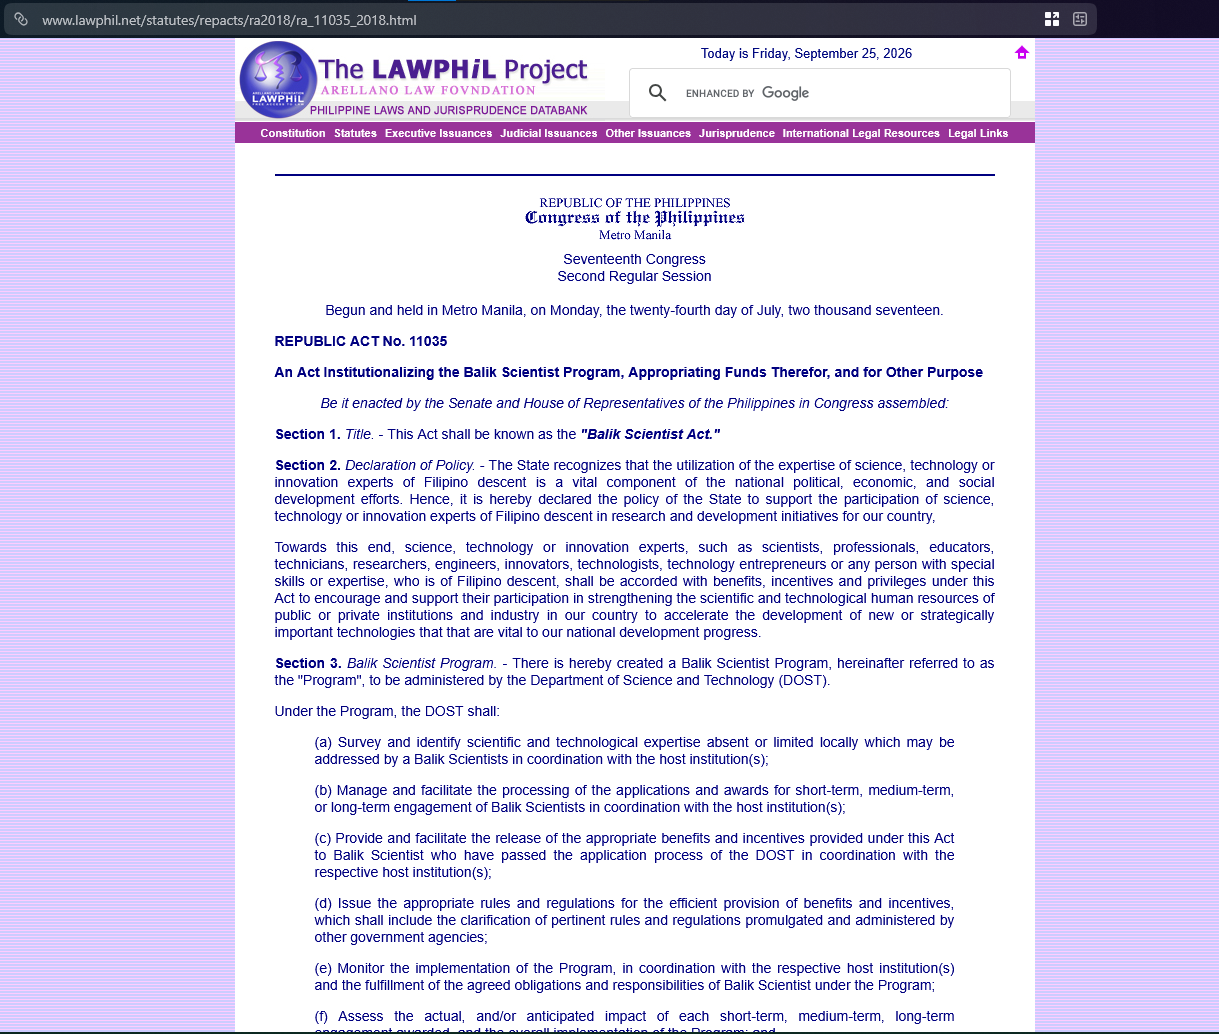
\includegraphics[width=0.92\linewidth]{figs/lawphil_republic_act_sample.png}
            \caption{Sample Statutory Enactment Webpage from the Lawphil Project Repository (Republic Act No.~11035, \textit{Balik Scientist Act}). The repository features a streamlined, clean HTML document layout without intrusive styling or dynamic client-side rendering. Furthermore, its transparent and predictable URL hierarchy (\texttt{/statutes/repacts/ra2018/ra\_11035\_2018.html}) systematically organizes enactments by instrument type, legislative year, and statutory numbering, enabling automated, fault-tolerant corpus harvesting.}
            \label{fig:lawphil_web_interface}
        \end{figure}

        \begin{lstlisting}[language=Python, caption={Code Snippet of the Statutory Corpus Acquisition and Provision Extraction Pipeline}, label={lst:corpus_extraction}]
def extract_statutory_corpus(base_url, start_year=1900, end_year=2026):
    """
    Extracts, sanitizes, and structures national statutes from the online archive.
    """
    statute_records = []
    
    for year in range(start_year, end_year + 1):
        year_index = fetch_page(f"{base_url}/year/{year}")
        statute_links = parse_index_links(year_index)
        
        for link in statute_links:
            # Fetch raw web page and parse HTML DOM tree
            html_content = fetch_page_with_retry(link, delay_seconds=1.0)
            soup = BeautifulSoup(html_content, "html.parser")
            
            # Extract statutory metadata and clean document body
            metadata = extract_header_metadata(soup)
            body_text = clean_document_body(soup)
            
            # Segment statute into discrete section-level provisions
            sections = segment_into_sections(body_text)
            
            record = {
                "statute_id": metadata.id,
                "title": metadata.title,
                "instrument": metadata.type,
                "date_enacted": metadata.date,
                "sections": sections
            }
            statute_records.append(record)
            
    return statute_records
        \end{lstlisting}

        Collecting national laws from Lawphil helps avoid the disorganization common to public legal websites. Although the Official Gazette and congressional websites also host statutory records, their web pages frequently change layout and often provide older laws only as image-only PDF scans. In contrast, Lawphil keeps a standard HTML structure across all historical eras, clearly separating introductory preambles from operative legal sections. Scraping from this repository ensured uniform text formatting across the national collection (over 25,000 enactments), preventing formatting differences from skewing vector embeddings during Stage~1 retrieval. The resulting collection provides a clean, consistent text foundation for semantic analysis and conflict detection.

        To capture the complete statutory search space, the national collection is paired with Davao City municipal legislation gathered across two complementary channels:
        \begin{enumerate}
            \item \textbf{Davao City SP Public Web Portal:} Provides historical ``Landmark Ordinances'' spanning approximately 15 years, capturing prominent regulatory codes in public safety, zoning, and health.
            \item \textbf{Legislative Information Support System Program (LISSP):} Acquired directly through formal coordination with the Sangguniang Panlungsod (SP) IT Department, providing approximately 1,000 digitized ordinances enacted between 2021 and 2026 (retrieved as of March 2026)~\cite{citygov2025lissp}.
        \end{enumerate}
        Together, these two channels yield an archive of approximately 1,500 local enactments. When combined with the 25k+ national statutes, the total statutory search space comprises \textbf{over 27,000+ legal enactments}. Unlike national statutes available in digital text, the local ordinances are scanned image-based PDF files currently undergoing optical character recognition (OCR) cleaning and text extraction led by co-author Ralph Paolo Dulce before downstream exploratory analysis.

        \subsubsection{Corpus Biases}
        A close look at the collected national laws reveals a large imbalance across legal topics. Over 40\% of the national statutes consist of routine administrative actions, such as converting local schools, renaming roads, adjusting municipal boundaries, or granting broadcast franchises. In contrast, major regulatory areas that interact with city powers, such as public health, land zoning, and local taxation, make up less than 15\% of the total national collection. Searching through this raw distribution without filtering would cause search algorithms to return irrelevant administrative laws instead of actual regulatory rules. To keep search results useful, the system must separate these routine administrative laws from substantive regulatory provisions.

        The municipal archive also shows an uneven time distribution and gaps in older records. For ordinances passed before 2021, city record-keeping mainly focused on digitizing major ``Landmark Ordinances,'' leaving ordinary regulations from earlier decades in physical paper storage~\cite{spdavao2026}. As a result, the pre-2021 local records represent a selective collection of prominent laws rather than a complete legislative record. While post-2021 records from the digital LISSP database are much more complete, some numerical gaps remain due to missing committee drafts and unindexed attachments. These gaps mean that the available municipal archive contains more recent ordinances than older ones.

        The physical state of the scanned city ordinances adds both visual and linguistic noise. Older ordinances scanned at low resolution suffer from faded print, ink smudges, and crooked pages, as illustrated in Figure~\ref{fig:davao_ordinance_scan}. The paper copies also contain non-text items such as government stamps, official signatures, and handwritten notes that confuse sentence splitting tools. At the language level, local ordinances sometimes include regional terms and administrative Taglish in their introductory sections~\cite{dreisbach2021language}. These informal drafting habits differ noticeably from the formal, standardized English found in national laws.

        \begin{figure}[!htbp]
            \centering
            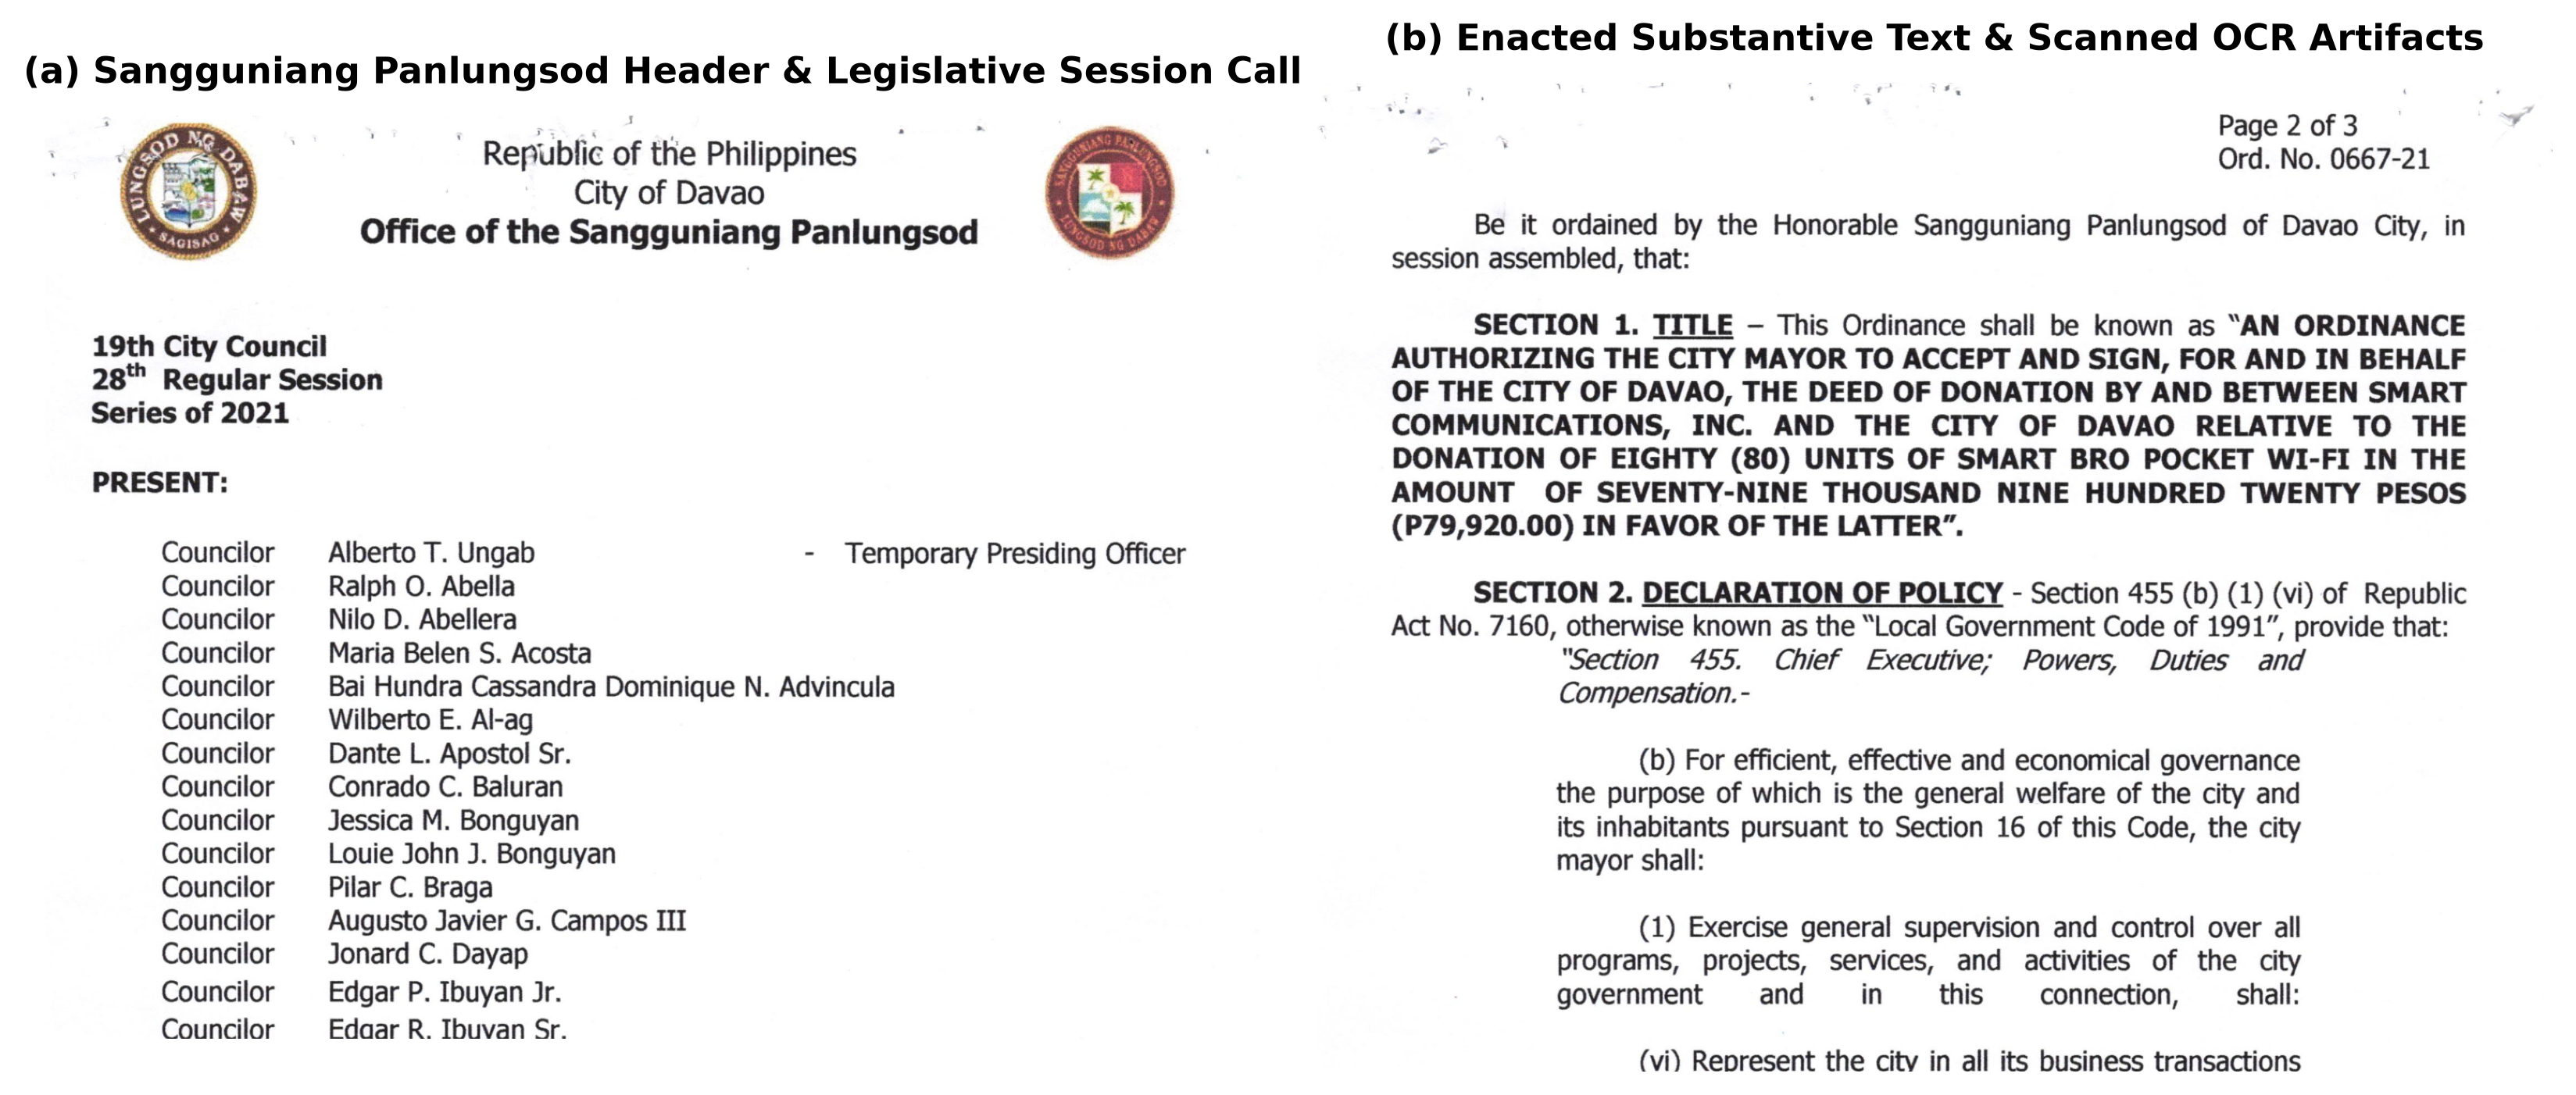
\includegraphics[width=0.96\linewidth]{figs/davao_ordinance_scan_sample.png}
            \caption{Sample Archival Document from the Davao City Sangguniang Panlungsod Corpus Illustrating Physical Scanning Artifacts and Optical Character Recognition (OCR) Noise. Panel (a) illustrates the official municipal session heading, seal, and city council metadata. Panel (b) shows the enacted substantive provisions exhibiting real OCR scanner noise, character substitutions (e.g., ``0667-2L'' for 2021, ``TITTE'' for Title), and document skew.}
            \label{fig:davao_ordinance_scan}
        \end{figure}

        In real-world legislation, direct contradictions between laws are very rare. Lawmakers generally try to write rules that work alongside existing higher laws rather than directly opposing them~\cite{fuller1964the}. As a result, actual legal conflicts make up less than 1\% of random pairs formed between municipal ordinances and national statutes. Taking random pairs of text from the unedited collections would lead to an overwhelming majority of unrelated pairs. A machine learning model trained on such unbalanced data could score 99\% nominal accuracy simply by guessing ``Neutral'' every time, while remaining unable to detect real legal conflicts.

        \subsubsection{Corpus Analysis}
        Across the five main types of legislation with sequential numbers, the collected corpus includes 19,683 statutes out of an estimated 20,246 historical laws, achieving a coverage rate of 97.22\%. When combined with the 5,749 Executive Orders from fifteen presidential administrations, the compiled national archive holds 25,432 out of about 26,451 total historical legal documents, reaching a national recall rate of 96.15\%. All official legislative totals reflect the chronological numbering sequence established by Congress and presidential records as of \textbf{March 2026}, where sequential Republic Acts reached Republic Act No.~12,313. Table~\ref{tab:statute_type_composition} provides a breakdown of the national corpus, comparing the collected documents with official legislative totals for each statutory type. Figure~\ref{fig:statute_type_composition} shows the share of each legal instrument in the archive, illustrating the large volume of executive orders alongside congressional acts.

        A key methodological decision in compiling this database is the explicit inclusion of \textbf{Executive Orders (EOs)} alongside congressional legislation. Under Article~VII, Section~17 of the 1987 Philippine Constitution and Book~III, Title~I, Chapter~2, Section~2 of the Administrative Code of 1987 (Executive Order No.~292)~\cite{philgov1987eo292}, Executive Orders are presidential acts providing rules of a general or permanent character in implementation or execution of constitutional or statutory mandates. Unlike Supreme Court decisions—which function as \textit{ex-post} judicial dispute resolutions settling private adversarial controversies under the doctrine of \textit{stare decisis} (Article~8, Civil Code)—Executive Orders operate as \textit{ex-ante}, forward-looking statutory instruments possessing the full force and effect of law. Furthermore, during both the Martial Law period (1972--1986) and the Revolutionary Government under the Freedom Constitution (Proclamation No.~3, 1986--1987), the President exercised direct legislative decree-making powers, enacting substantive national rules that remain active law today. Modern Executive Orders establish binding nationwide regulatory mandates—such as Executive Order No.~26 (s.~2017) mandating nationwide public smoking bans, or Executive Order No.~168 (s.~2014) creating the IATF with binding quarantine standards—that legally preempt inconsistent local ordinances. Excluding Executive Orders would create an artificial regulatory vacuum, allowing local ordinances to contradict operative presidential mandates.

        \begin{table}[!htbp]
            \centering
            \footnotesize
            \setlength{\tabcolsep}{3.8pt}
            \caption{Comparative Statutory Coverage and Composition of the Philippine National Legal Archive ($N = 25,432$)}
            \label{tab:statute_type_composition}
            \begin{tabularx}{\linewidth}{c>{\RaggedRight}p{2.85cm}rrrr>{\RaggedRight}X}
                \toprule
                \textbf{ID} & \shortstack[l]{\textbf{Statutory}\\\textbf{Instrument}} & \textbf{Corpus} & \shortstack[r]{\textbf{Official}\\\textbf{Total}} & \shortstack[r]{\textbf{Coverage}\\\textbf{Rate}} & \shortstack[r]{\textbf{Corpus}\\\textbf{Share}} & \textbf{Historical Era and Governing Authority} \\
                \midrule
                01 & Republic Acts (RA) & 11,963 & 12,313 & 97.16\% & 47.04\% & Post-war and Fifth Republic legislation (1946--present, up to RA 12313 as of March 2026) \\
                02 & Executive Orders (EO) & 5,749 & 6,205\textsuperscript{*} & 92.65\% & 22.61\% & Presidential administrative issuances (1901--2026, across 15 administrations) \\
                03 & Acts & 4,257 & 4,275 & 99.58\% & 16.74\% & American Insular Government enactments (1900--1935) \\
                04 & Presidential Decrees (PD) & 1,844 & 2,036 & 90.57\% & 7.25\% & Martial law legislative decrees enacted by executive fiat (1972--1986) \\
                05 & Batas Pambansa (BP) & 886 & 889 & 99.66\% & 3.48\% & Unicameral parliamentary legislation under the 1973 Constitution \\
                06 & Commonwealth Acts (CA) & 733 & 733 & 100.00\% & 2.88\% & Transitional governance enactments under the 1935 Constitution \\
                \midrule
                \multicolumn{2}{l}{\textbf{Sequential Subtotal}} & \textbf{19,683} & \textbf{20,246} & \textbf{97.22\%} & \textbf{77.39\%} & \textbf{All numbered legislative enactments of Congress} \\
                \multicolumn{2}{l}{\textbf{Total Archive}} & \textbf{25,432} & \textbf{26,451} & \textbf{96.15\%} & \textbf{100.00\%} & \textbf{Comprehensive corpus extracted from the Lawphil Project} \\
                \bottomrule
                \multicolumn{7}{p{0.97\linewidth}}{\scriptsize \textsuperscript{*}Historical total for Executive Orders represents the aggregate sum of maximum numbered issuances across all fifteen presidential administrations (1935--2026) and colonial governorships (1901--1935) as recorded in the Official Gazette and Lawphil archives as of March 2026.}
            \end{tabularx}
        \end{table}

        \begin{figure}[!htbp]
            \centering
            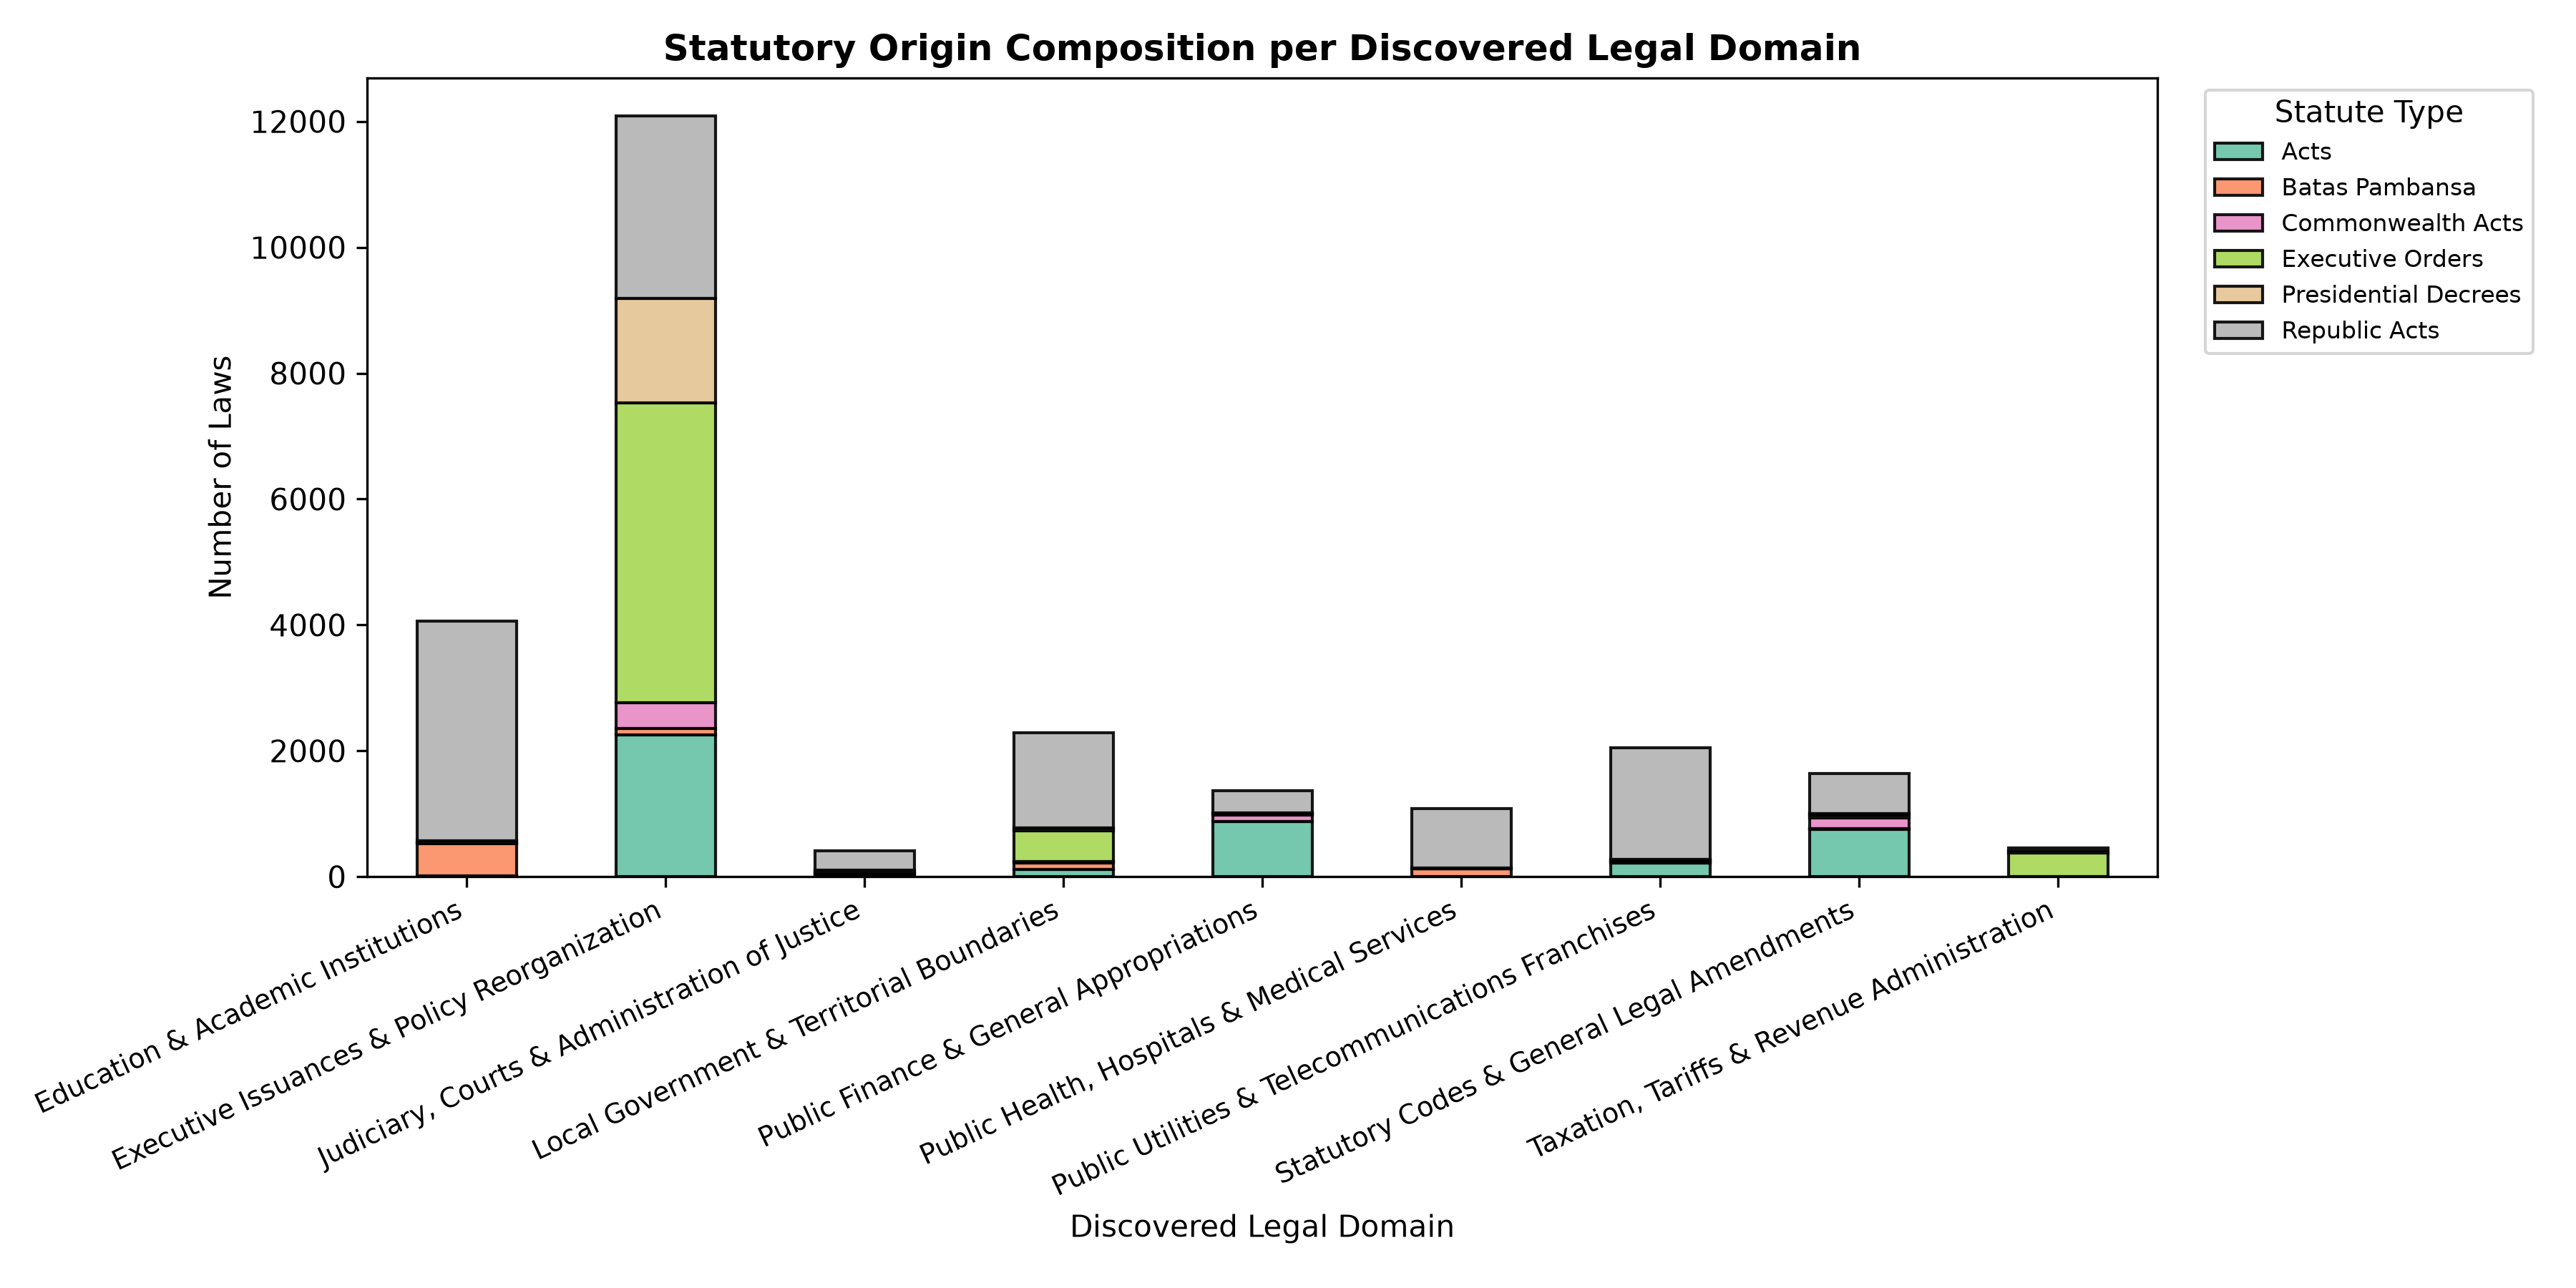
\includegraphics[width=0.78\linewidth]{figs/statute_type_composition.png}
            \caption{Composition of the Philippine National Statutory Corpus by Legislative Instrument ($N = 25,432$).}
            \label{fig:statute_type_composition}
        \end{figure}

        The coverage rates confirm that the national legal archive is nearly complete. Commonwealth Acts show full 100.00\% coverage across all 733 enactments, while American-era Acts (99.58\%) and Batas Pambansa (99.66\%) miss only 18 and 3 enactments, respectively. For Republic Acts, the 11,963 collected records cover 97.16\% of the 12,313 official total, with missing entries mainly being local bills or recent laws still being indexed. For Presidential Decrees, the 1,844 gathered records represent 90.57\% of the 2,036 numbered decrees from the Martial Law period, where uncollected entries were unpublished directives until the Supreme Court required full publication in \textit{Tañada v. Tuvera}~\cite{sc1985tanadavtuvera}. For Executive Orders, the 5,749 collected records represent 92.65\% of the 6,205 numbered orders issued across fifteen presidential terms, offering an extensive record of administrative policy.

        This breakdown also explains why executive and administrative orders account for nearly half (48.01\%) of the subsequent topic groups. Executive Orders (22.61\%) and Presidential Decrees (7.25\%) together make up 7,593 documents, representing nearly one-third of the entire national archive. When combined with colonial-era civil administration Acts and agency reorganizations, administrative directives form the largest single category of Philippine legal text. In language processing, this large volume of administrative text poses a challenge during search, as queries can easily match routine bureaucratic language rather than municipal regulations. This reality shows why automated topic grouping is needed to keep local ordinance checks focused on relevant laws.

        To trace how the six statutory instruments evolved across Philippine jurisprudence, the proponents categorized statutory enactments across six chronological eras. Each historical era established distinct legislative authorities, ranging from colonial commissions to modern constitutional congresses. Figure~\ref{fig:historical_temporal_evolution} charts the chronological succession and aggregate volume of statutory instruments from 1900 through 2026. The distribution reflects the shifting primacy of legislative acts, presidential decrees, and administrative executive orders across political transitions. Examining these enactment waves illustrates how historical governance structures directly shaped the composition of the national legal corpus.

        \begin{figure}[htbp]
            \centering
            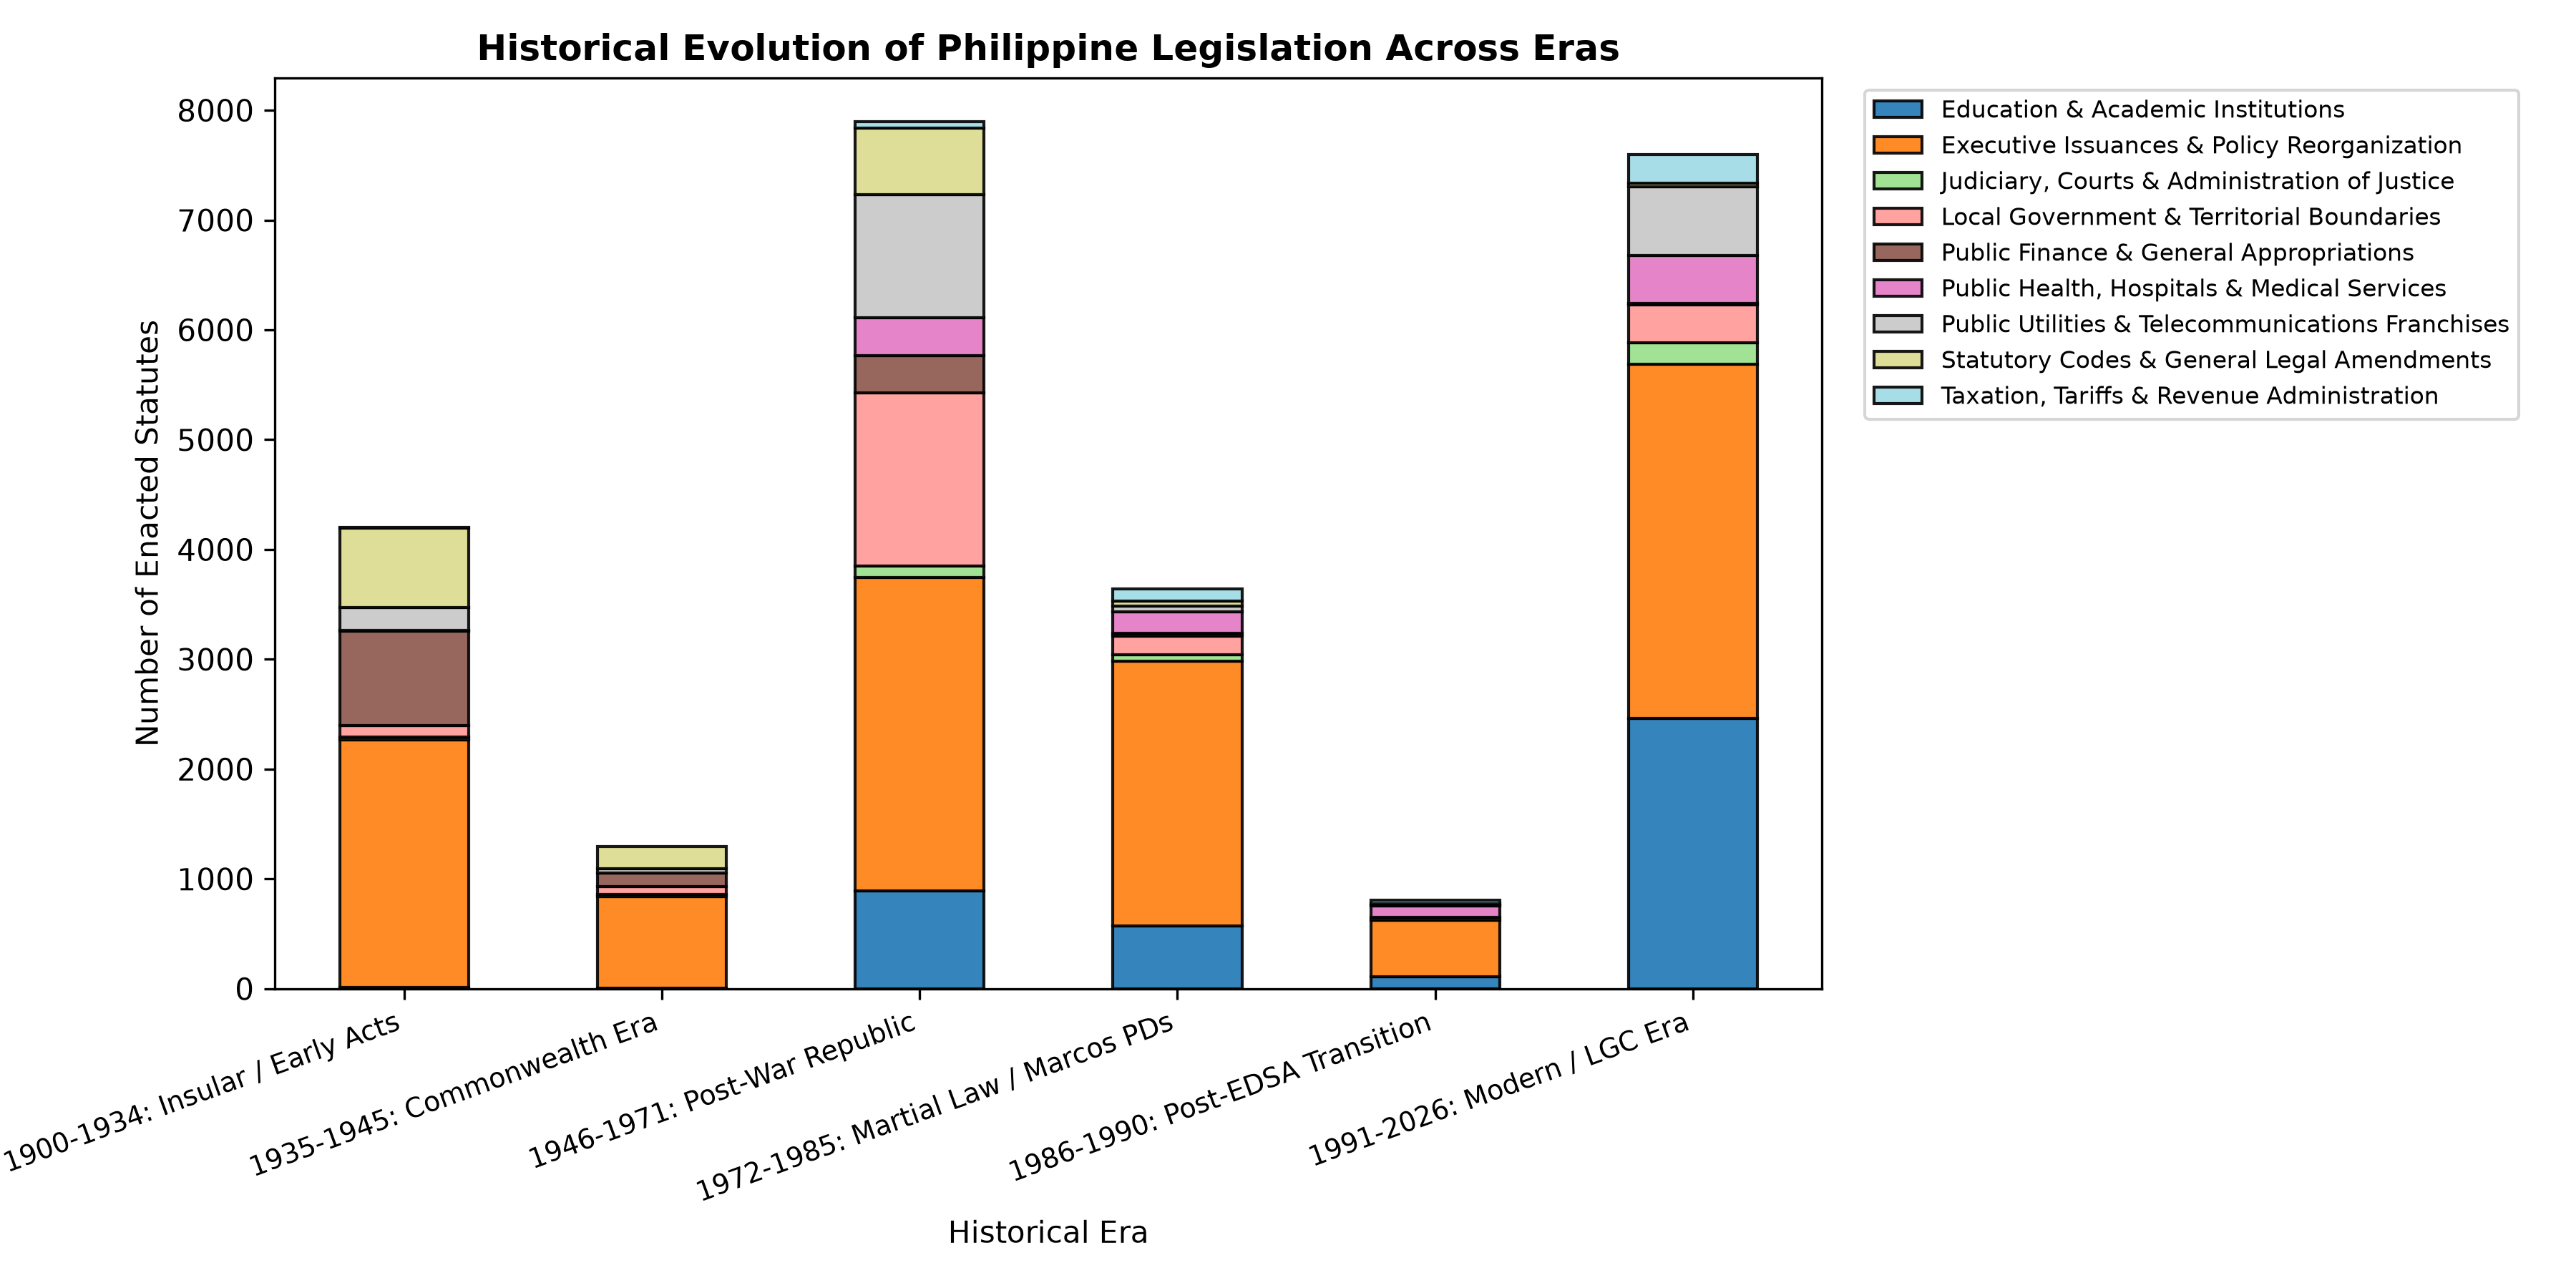
\includegraphics[width=0.96\linewidth]{figs/historical_temporal_evolution.png}
            \caption{Historical Succession and Volume of Statutory Instruments across Six Chronological Eras (1900--2026, $N = 25,432$).}
            \label{fig:historical_temporal_evolution}
        \end{figure}

        The temporal breakdown reveals that Philippine lawmaking expanded during periods of national administrative reorganization. Early colonial governance relied entirely on 4,199 foundational Acts during the Insular period (1900--1934). Centralized presidential lawmaking predominated during the Martial Law period through 1,844 Presidential Decrees and 886 Batas Pambansa parliamentary enactments (1972--1985). In the modern era governed by Republic Act No.~7160 (1991--2026), statutory production stabilized into a dual stream of 4,900 congressional Republic Acts and 2,421 executive policy orders. Because vocabulary standards shifted markedly across these legislative transitions, search models require chronological awareness to avoid misinterpreting historical statutory phrasing.

    \subsection{Preprocessing and Filtering}
    \label{sec:preprocessing_filtering}
    Because the raw downloaded files vary widely in formatting, they require thorough cleaning, grouping, and text normalization. While national statutes are already available as clean digital text, the scanned Davao City ordinances contain most of the OCR errors in the dataset. Since these local records come from image-based PDFs, extracting the text often produces misread characters and broken lines. The pipeline uses rule-based filters to find and correct these errors specifically within the local ordinance files. This targeted cleaning ensures that the subsequent vector conversion process is not disrupted by broken words or garbled text.

        \subsubsection{Digital-Born Draft Ingestion and Section Segmentation}
        \label{sec:draft_ingestion_segmentation}
        A critical operational distinction in this research separates the historical training archive from live ex-ante draft submissions. While the historical Davao City collection (~1,660 enactments from 1946 to 2025) consists of scanned physical PDFs requiring intensive optical character recognition (OCR) and text normalization, newly drafted ordinances submitted for ex-ante review are digital-born documents. Legislative staff create these proposed measures using standard word processing software, generating clean electronic text or searchable PDF files. Because digital-born drafts contain authentic character encodings without scanning artifacts, the live pipeline bypasses OCR error correction entirely. This structural decoupling allows the preprocessor to focus immediately on automated section boundary parsing and clause segmentation.

        To evaluate legislative commands without semantic distortion, an automated regular expression parser splits the submitted draft at formal section boundaries into discrete operative blocks. In Philippine local legislative practice, proposed measures follow standardized structural templates established by the Department of the Interior and Local Government~\cite{dilg2022drafting}. However, real-world legislative drafts contain substantial procedural boilerplate that does not express substantive legal commands. If routine clauses such as title declarations, repealing clauses, and effectivity dates are fed into Stage~1 retrieval, they match thousands of administrative national statutes containing similar formulaic phrases. To prevent search drift and computational waste, the preprocessor automatically filters out non-operative sections---specifically Title, Separability, Repealing, and Effectivity clauses---directing candidate retrieval exclusively toward substantive regulatory and penal provisions.

        Listing~\ref{lst:jsonl_sample} displays an authentic raw ingestion record from the scraped national statutory collection (\texttt{corpus/national\_laws/republic\_acts.jsonl}), capturing the raw unparsed text, enactment year, and source URL for Republic Act No.~11035 (\textit{Balik Scientist Act}, matching the Lawphil page illustrated in Figure~\ref{fig:lawphil_web_interface}). Listing~\ref{lst:provision_extractor} details the regular expression parser that segments live draft measures into discrete operative sections while filtering out procedural boilerplate.

        \begin{lstlisting}[language=Python, caption={Sample Raw JSONL Ingestion Record from the National Statutory Archive (Republic Act No. 11035)}, label={lst:jsonl_sample}]
# Raw Ingestion Record from corpus/national_laws/republic_acts.jsonl (ra_11035_2018)
raw_statute_record = {
    "law_id": "ra_11035_2018",
    "year": 2018,
    "url": "https://lawphil.net/statutes/repacts/ra2018/ra_11035_2018.html",
    "scraped_at": "2026-02-17T18:44:04.745654",
    "text": (
        "Seventeenth Congress\nSecond Regular Session\nBegun and held in Metro Manila, "
        "on Monday, the twenty-fourth day of July, two thousand seventeen.\n"
        "REPUBLIC ACT No. 11035\n"
        "An Act Institutionalizing the Balik Scientist Program, Appropriating Funds "
        "Therefor, and for Other Purpose\n"
        "Be it enacted by the Senate and House of Representatives of the Philippines "
        "in Congress assembled:\n"
        "Section 1. Title. - This Act shall be known as the \"Balik Scientist Act.\"\n"
        "Section 2. Declaration of Policy. - The State recognizes that the utilization "
        "of the expertise of science, technology or innovation experts of Filipino descent "
        "is a vital component of the national political, economic, and social development "
        "efforts...\n"
        "Section 3. Balik Scientist Program. - There is hereby created a Balik Scientist "
        "Program, hereinafter referred to as the \"Program\", to be administered by the "
        "Department of Science and Technology (DOST)...\n"
        "[Raw statutory text continues across 2,493 total words]"
    )
}
        \end{lstlisting}

        \begin{lstlisting}[language=Python, caption={Code Snippet of the Operative Provision Extractor and Boilerplate Filter}, label={lst:provision_extractor}]
import re

def extract_operative_provisions(draft_text):
    """
    Parses digital-born draft ordinance into discrete sections,
    filtering out non-operative procedural boilerplate clauses.
    """
    # Regex pattern to segment text at formal section boundaries
    pattern = r'(SECTION\s+\d+\.?[^\n]*\n.*?)(?=(?:SECTION\s+\d+|CERTIFIED|ENACTED|\Z))'
    matches = re.findall(pattern, draft_text, re.DOTALL | re.IGNORECASE)
    
    # Procedural clauses that do not carry substantive regulatory commands
    boilerplate_keywords = ["TITLE", "SEPARABILITY", "REPEALING", "EFFECTIVITY"]
    operative_sections = []
    
    for match in matches:
        clean_chunk = ' '.join(match.strip().split())
        header = clean_chunk.split('.')[0] if '.' in clean_chunk else clean_chunk[:30]
        
        # Exclude non-operative procedural boilerplate
        if any(kw in header.upper() for kw in boilerplate_keywords):
            continue
            
        operative_sections.append({
            "section_header": header,
            "operative_text": clean_chunk
        })
        
    return operative_sections
        \end{lstlisting}

        Once operative sections are isolated, evaluating granular statutory provisions requires preserving their governing legislative identity. An isolated sub-clause (such as a standalone penalty statement) stripped of its parent enactment number and title suffers from severe semantic vector dilution, causing retrieval models to confuse municipal regulatory penalties with unrelated national tax or criminal codes. To maintain semantic precision and hierarchy across both stages, the pipeline applies structural context prepending. Listing~\ref{lst:context_prepending} details the context prepending protocol, while Listing~\ref{lst:model_ready_chunk} demonstrates the concrete transformation from an isolated provision into a Stage~1 indexed chunk and the resulting Stage~2 asymmetric input sequence.

        \begin{lstlisting}[language=Python, caption={Pseudocode of the Section Context Prepending Protocol for Granular Provision Chunking}, label={lst:context_prepending}]
def prepend_statutory_context(statute_record, section):
    """
    Prepends governing legislative identity to isolated section text
    to prevent semantic vector dilution and preserve hierarchical rank.
    """
    prefix = (
        f"[{statute_record['instrument_type']} No. {statute_record['enactment_number']}: "
        f"{statute_record['title']} | {section['section_number']}: {section['section_title']}] "
    )
    model_ready_text = prefix + section['raw_text']
    return model_ready_text
        \end{lstlisting}

        \begin{lstlisting}[language=Python, caption={Sample Model-Ready Statutory Chunk and Stage 2 Input Sequence with Context Prepending}, label={lst:model_ready_chunk}]
# 1. Isolated Statutory Provision (Without Context Prepending)
# Lacks parent statutory identity; dense embeddings match ambiguous administrative powers.
isolated_section = (
    "Section 458. (a) The sangguniang panlungsod, as the legislative body of the city, "
    "shall enact ordinances... (v) Approve ordinances which shall impose a fine not "
    "exceeding Five thousand pesos (P5,000.00) or an imprisonment not exceeding one (1) "
    "year, or both."
)

# 2. Model-Ready Contextualized Provision Chunk (Indexed by Stage 1 BM25 & Dense Bi-Encoders)
# Prepends statutory title and citation to establish legal hierarchy and topical specificity.
stage1_indexed_chunk = (
    "[Republic Act No. 7160: Local Government Code of 1991 | Section 458: Powers, Duties, "
    "and Functions of the Sangguniang Panlungsod] Section 458. (a) The sangguniang panlungsod, "
    "as the legislative body of the city, shall enact ordinances... (v) Approve ordinances which "
    "shall impose a fine not exceeding Five thousand pesos (P5,000.00) or an imprisonment not "
    "exceeding one (1) year, or both."
)

# 3. Assembled Asymmetric Input Sequence Passed to Stage 2 Cross-Encoder
# Formatted with [CLS] and [SEP] tokens pairing governing premise with proposed draft hypothesis.
stage2_input_sequence = (
    "[CLS] Premise: [Republic Act No. 7160: Local Government Code of 1991 | Section 458: "
    "Powers of the Sangguniang Panlungsod] Section 458. (a)... Approve ordinances which shall "
    "impose a fine not exceeding Five thousand pesos (P5,000.00)... "
    "[SEP] Hypothesis: [Proposed Davao City Ordinance No. 2024-012 | Section 6: Penalties] "
    "SECTION 6. PENALTY CLAUSE. Any person violating this Ordinance shall be penalized with "
    "a fine of Fifteen Thousand Pesos (PHP 15,000.00) or two years imprisonment. [SEP]"
)
        \end{lstlisting}

        \subsubsection{Domain Categorization}
        \label{sec:domain_categorization}
        During preliminary exploratory research, the proponents conducted initial machine learning experiments on the national statutory archive and identified severe dataset imbalances. In the national collection of 25,432 statutes, routine executive issuances and administrative reorganizations comprise nearly half of all historical enactments, while specialized regulatory domains remain relatively small. Searching for a local regulatory ordinance across this raw, unfiltered collection causes severe search drift because dense retrieval models readily match repetitive administrative phrasing across unrelated legal areas. To resolve these dataset quirks, the proponents formalized a two-stage topic modeling architecture that organizes the statutory archive into cohesive, well-separated subject areas. This structured categorization prevents routine administrative directives from crowding the candidate shortlist during coarse retrieval, establishing a balanced foundation for subsequent conflict checks.

        The topic classification pipeline groups documents automatically while running smoothly on standard local computers. First, the 25,432 statutory texts are cleaned by removing HTML tags and routine metadata. The pipeline removes a custom list of 49 common legal stopwords, such as ``hereby,'' ``enacted,'' and ``republic,'' which appear in almost every law without helping identify its specific topic. Second, the cleaned texts are converted into term frequency-inverse document frequency (TF-IDF) feature vectors, capped at a vocabulary of 25,000 single words and two-word phrases. In text mining and information retrieval, TF-IDF is a statistical weighting that measures the relative importance of a term within a document relative to an entire corpus; it rewards words that appear frequently within a particular statute while penalizing ubiquitous terms that appear indiscriminately across the broader archive~\cite{manning2008introduction}. To keep calculations fast on local hardware while preserving conceptual cohesion, the pipeline uses Truncated Singular Value Decomposition (SVD) to project the sparse word vectors into 64 latent semantic dimensions~\cite{deerwester1990indexing}. In latent semantic modeling, Landauer et al.~\cite{landauer1998introduction} established that projecting vocabulary matrices into a 50-to-300 dimensional latent subspace captures underlying semantic associations while filtering out high-frequency lexical noise and idiosyncratic drafting variations. This is followed by standard $L_2$ vector normalization.

        Grouping legal texts directly into a small number of broad topics risks mixing very different types of laws together. To avoid this problem, the normalized 64-dimensional vectors are first divided into $K = 28$ smaller micro-clusters using MiniBatch $K$-Means clustering~\cite{sculley2010webscale}. Following the over-clustering strategy recommended by Grootendorst~\cite{grootendorst2022bertopic} and Aggarwal~\cite{aggarwal2012mining}, setting an over-complete cluster space ($K \approx 20\text{--}30$) isolates repetitive narrow enactments, such as school conversions or telecom franchises, into tight individual clusters before macro consolidation. Next, the pipeline adapts the class-based TF-IDF ($c\text{-}TF\text{-}IDF$) method from Grootendorst~\cite{grootendorst2022bertopic} to find the most representative keywords for each group. By treating all text within a micro-cluster as a single combined document, $c\text{-}TF\text{-}IDF$ measures how important a word is to that specific cluster compared to the rest of the collection:

        \[
            c\text{-}TF\text{-}IDF_{i, c} = \frac{|t_{i, c}|}{|c|} \times \log\left(1 + \frac{A}{\sum_{k} |t_{i, k}|}\right)
        \]
        where $|t_{i, c}|$ represents the absolute frequency of word $i$ within cluster $c$, $|c|$ denotes the total word count of cluster $c$, and $A$ indicates the mean word count per cluster across the full collection.

        In order to connect these mathematical clusters to real legal subjects, the extracted $c\text{-}TF\text{-}IDF$ keywords are matched against a curated Philippine legal taxonomy. This taxonomy reflects the main local government duties and regulatory powers outlined in the Local Government Code of 1991~\cite{philgov1991ra7160}. Micro-clusters that share the same general legal topic are merged into consolidated macro domains. To remove minor edge cases, the pipeline requires each macro domain to contain at least 1.0\% of the corpus ($N \ge 254$ statutes). Micro-clusters that fall below this cutoff are reassigned to their nearest semantic center, ensuring each macro domain has enough documents for reliable search indexing:

        \[
            \mathbf{C}_m = \frac{\sum_{i \in \mathcal{D}_m} \mathbf{z}_i}{\left\|\sum_{i \in \mathcal{D}_m} \mathbf{z}_i\right\|_2}, \quad P(m \mid \mathbf{z}_i) = \frac{\exp(\tau \cdot \cos(\mathbf{z}_i, \mathbf{C}_m))}{\sum_{j} \exp(\tau \cdot \cos(\mathbf{z}_i, \mathbf{C}_j))}
        \]
        where $\mathbf{z}_i$ represents the normalized 64-dimensional SVD vector of document $i$, $\mathbf{C}_m$ denotes the normalized centroid of macro domain $m$, and $\tau = 6.0$ functions as the inverse temperature scaling parameter governing prediction confidence. Adapting temperature scaling principles from Guo et al.~\cite{guo2017calibration}, this scaling factor prevents uncalibrated softmax dispersion across high-dimensional cosine distances, ensuring that dominant domain probabilities are sharply delineated without over-confident saturation.

        Running this topic grouping workflow across all 25,432 national statutes organizes the historical collection into eight Consolidated Macro Legal Domains. Table~\ref{tab:national_macro_domains} lists the final distribution, showing document counts, percentages, and the most descriptive keywords for each domain. Figure~\ref{fig:macro_domain_distribution} illustrates the relative size of each discovered macro domain.

        \begin{table}[htbp]
            \centering
            \footnotesize
            \caption{Consolidated Macro Legal Domains of the Philippine National Statutory Corpus ($N = 25,432$)}
            \label{tab:national_macro_domains}
            \begin{tabularx}{\linewidth}{r>{\RaggedRight}p{5.8cm}rr>{\RaggedRight}X}
                \toprule
                \textbf{ID} & \textbf{Consolidated Macro Domain} & \textbf{Statutes} & \textbf{Share} & \textbf{Top Salient $c\text{-}TF\text{-}IDF$ Keywords} \\
                \midrule
                00 & Executive Issuances \& Policy Reorganization & 12,210 & 48.01\% & executive, commission, committee, policy, code \\
                01 & Education \& Academic Institutions & 3,492 & 13.73\% & high school, elementary school, campus, college \\
                02 & Local Government \& Territorial Boundaries & 2,134 & 8.39\% & barangay, municipality, boundary, sitio, territorial \\
                03 & Public Utilities \& Telecom Franchises & 2,041 & 8.03\% & franchise, broadcast, telecommunications, radio \\
                04 & Public Health, Hospitals \& Medical Services & 1,890 & 7.43\% & hospital, bed capacity, medical center, infirmary \\
                05 & Statutory Codes \& General Legal Amendments & 1,873 & 7.36\% & administrative code, revised, amend, article, penalty \\
                06 & Public Finance \& General Appropriations & 1,335 & 5.25\% & appropriation, treasury, funds, expenditures \\
                07 & Taxation, Tariffs \& Revenue Administration & 457 & 1.80\% & tariff, customs code, internal revenue, excise \\
                \midrule
                \multicolumn{2}{l}{\textbf{Total Consolidated National Corpus}} & \textbf{25,432} & \textbf{100.00\%} & \textbf{All Enacted Statutes (1900--2026)} \\
                \bottomrule
            \end{tabularx}
        \end{table}

        \begin{figure}[htbp]
            \centering
            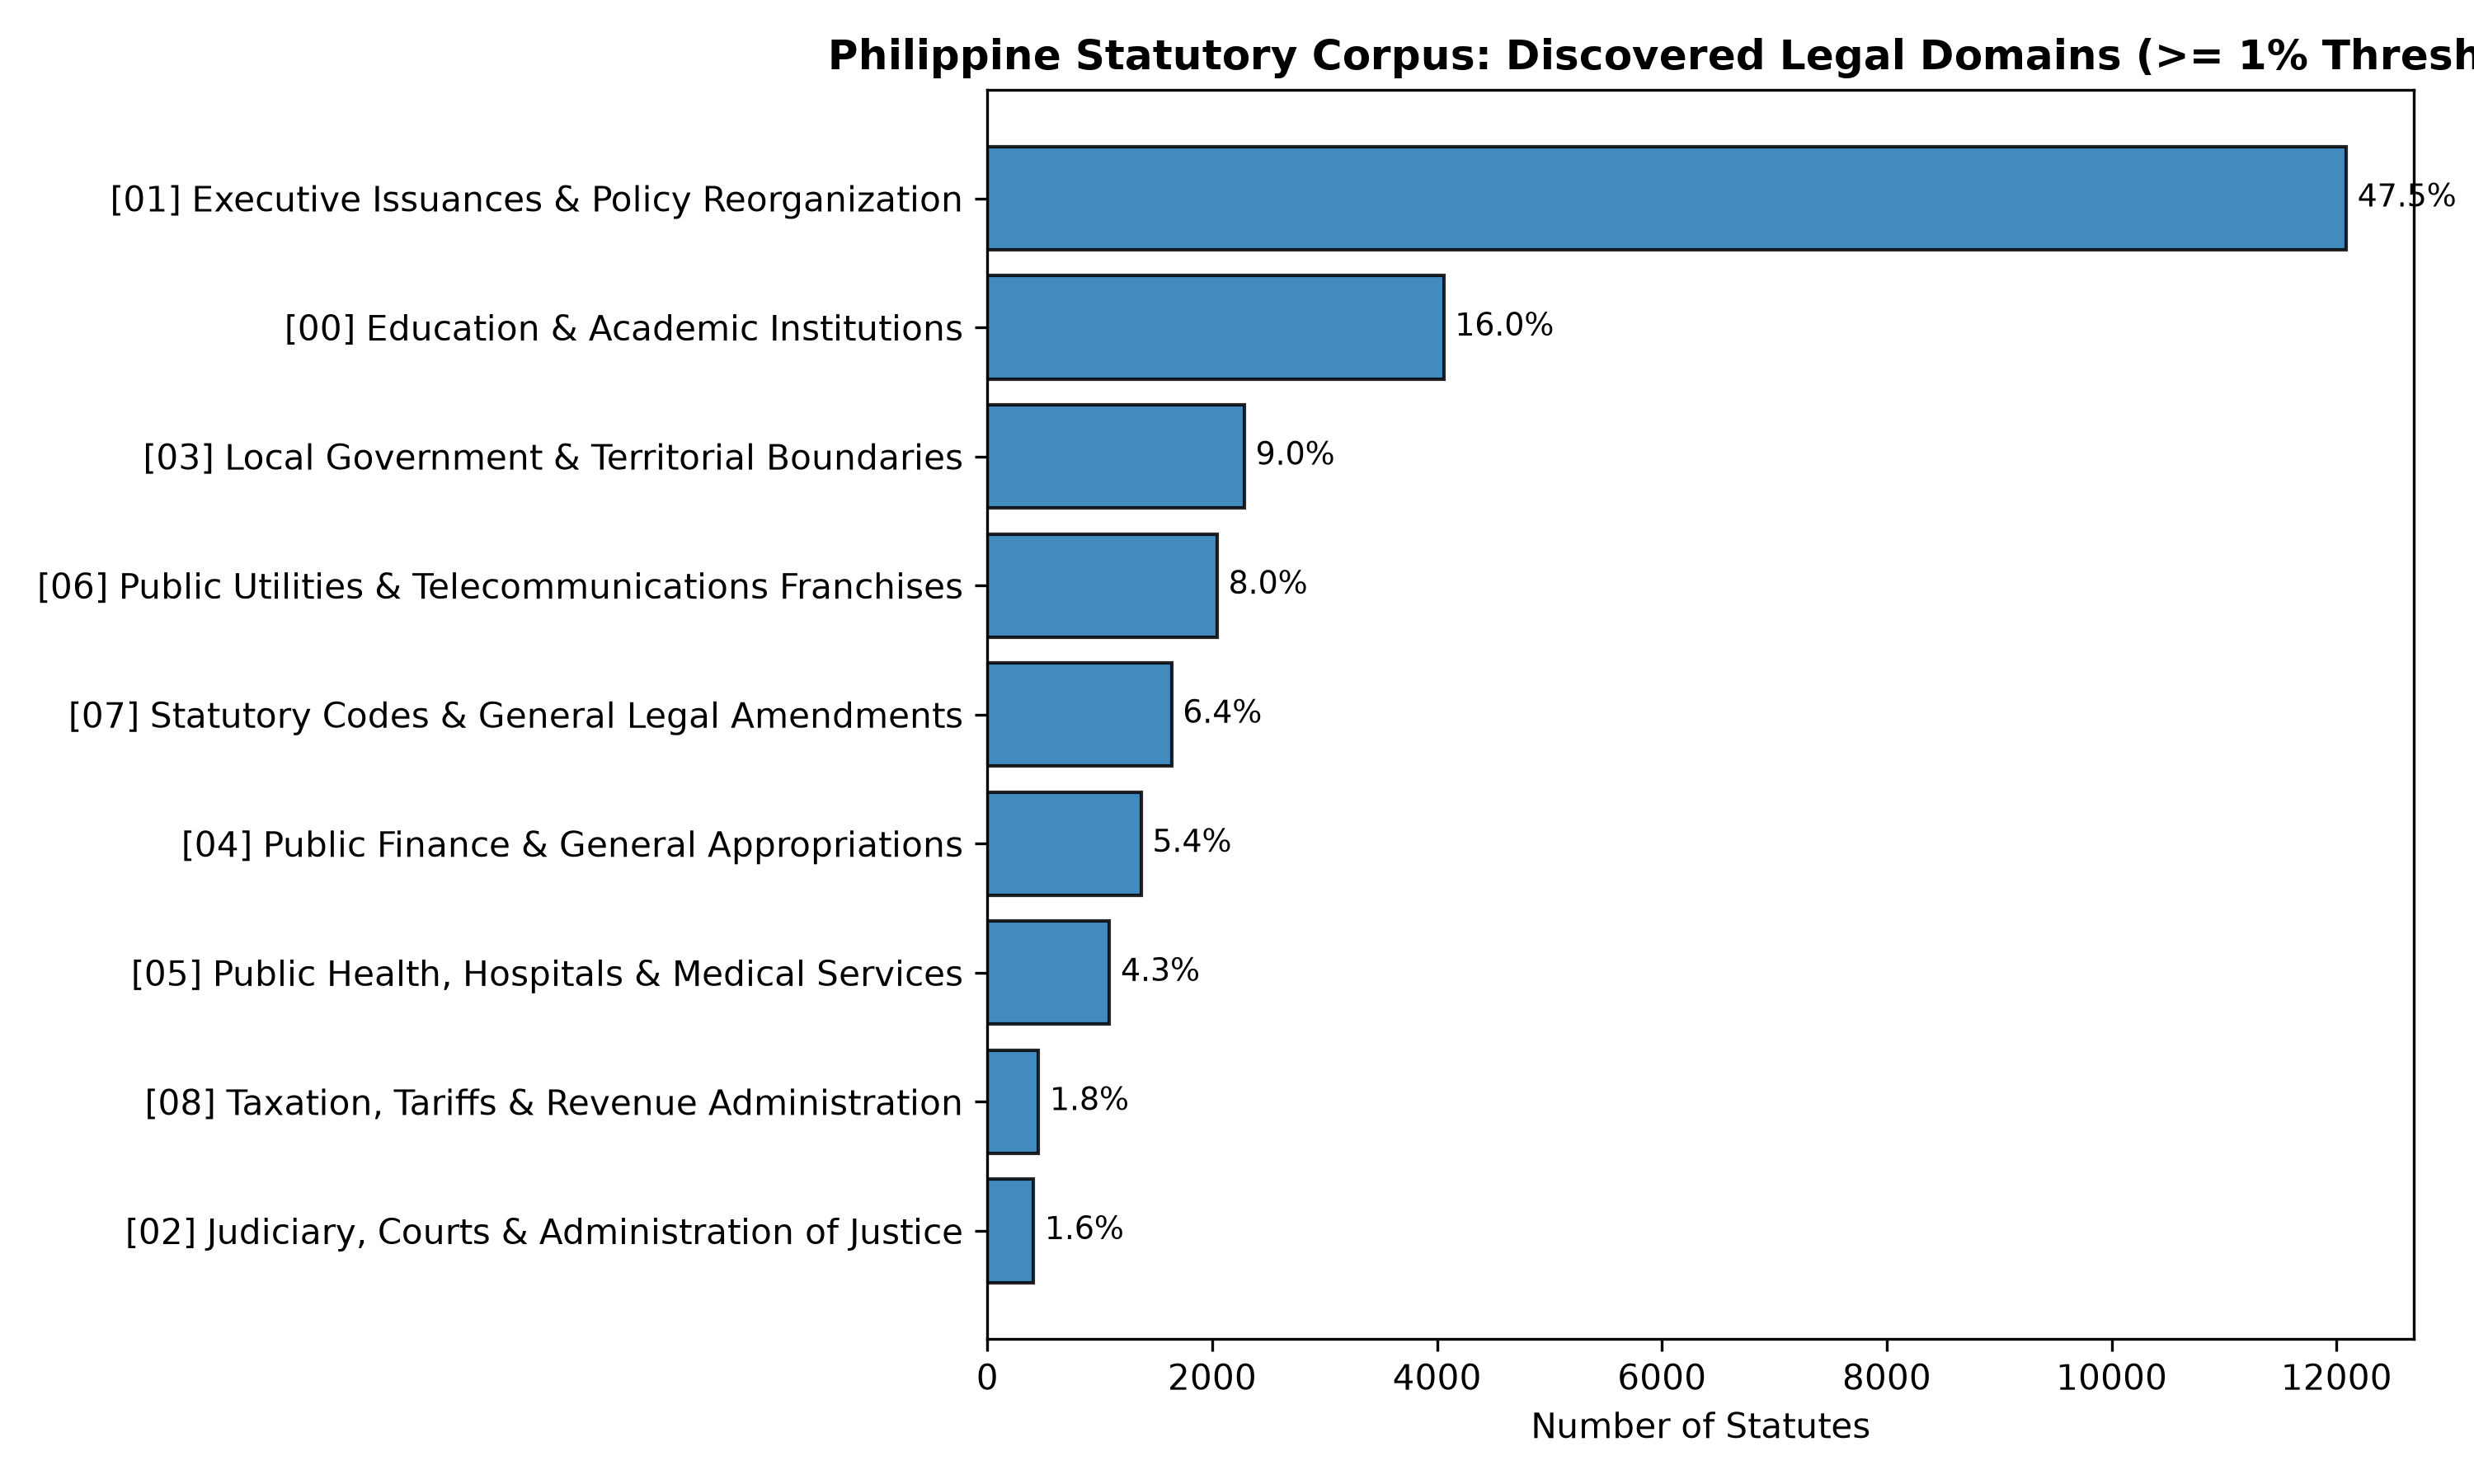
\includegraphics[width=0.88\linewidth]{figs/macro_domain_distribution.png}
            \caption{Distribution of the 25,432 Philippine National Statutes across the Consolidated Macro Legal Domains.}
            \label{fig:macro_domain_distribution}
        \end{figure}

        The topic distribution reflects the historical patterns of Philippine lawmaking. Executive issuances, administrative orders, and presidential decrees make up nearly half of the entire statutory collection, reflecting centralized authority during past political transitions. Common municipal subjects, including school infrastructure (13.73\%) and public utility franchises (8.03\%), form large distinct clusters with repetitive drafting patterns. In contrast, key regulatory topics like taxation (1.80\%) and public health (7.43\%) occupy smaller, highly focused portions of the database. Separating these regulatory clusters keeps routine administrative orders from crowding the candidate list during Stage~1 retrieval.

        To examine the geometric separation of these legal topics, the proponents projected the 64-dimensional SVD document vectors into a two-dimensional latent semantic landscape. Dimensionality reduction maps document similarities onto coordinate axes, allowing direct visual inspection of cluster cohesion. Figure~\ref{fig:semantic_topic_landscape_2d} illustrates this topic landscape across a representative stratified sample ($N = 3,500$), highlighting the core clusters and their spatial distributions.

        \begin{figure}[htbp]
            \centering
            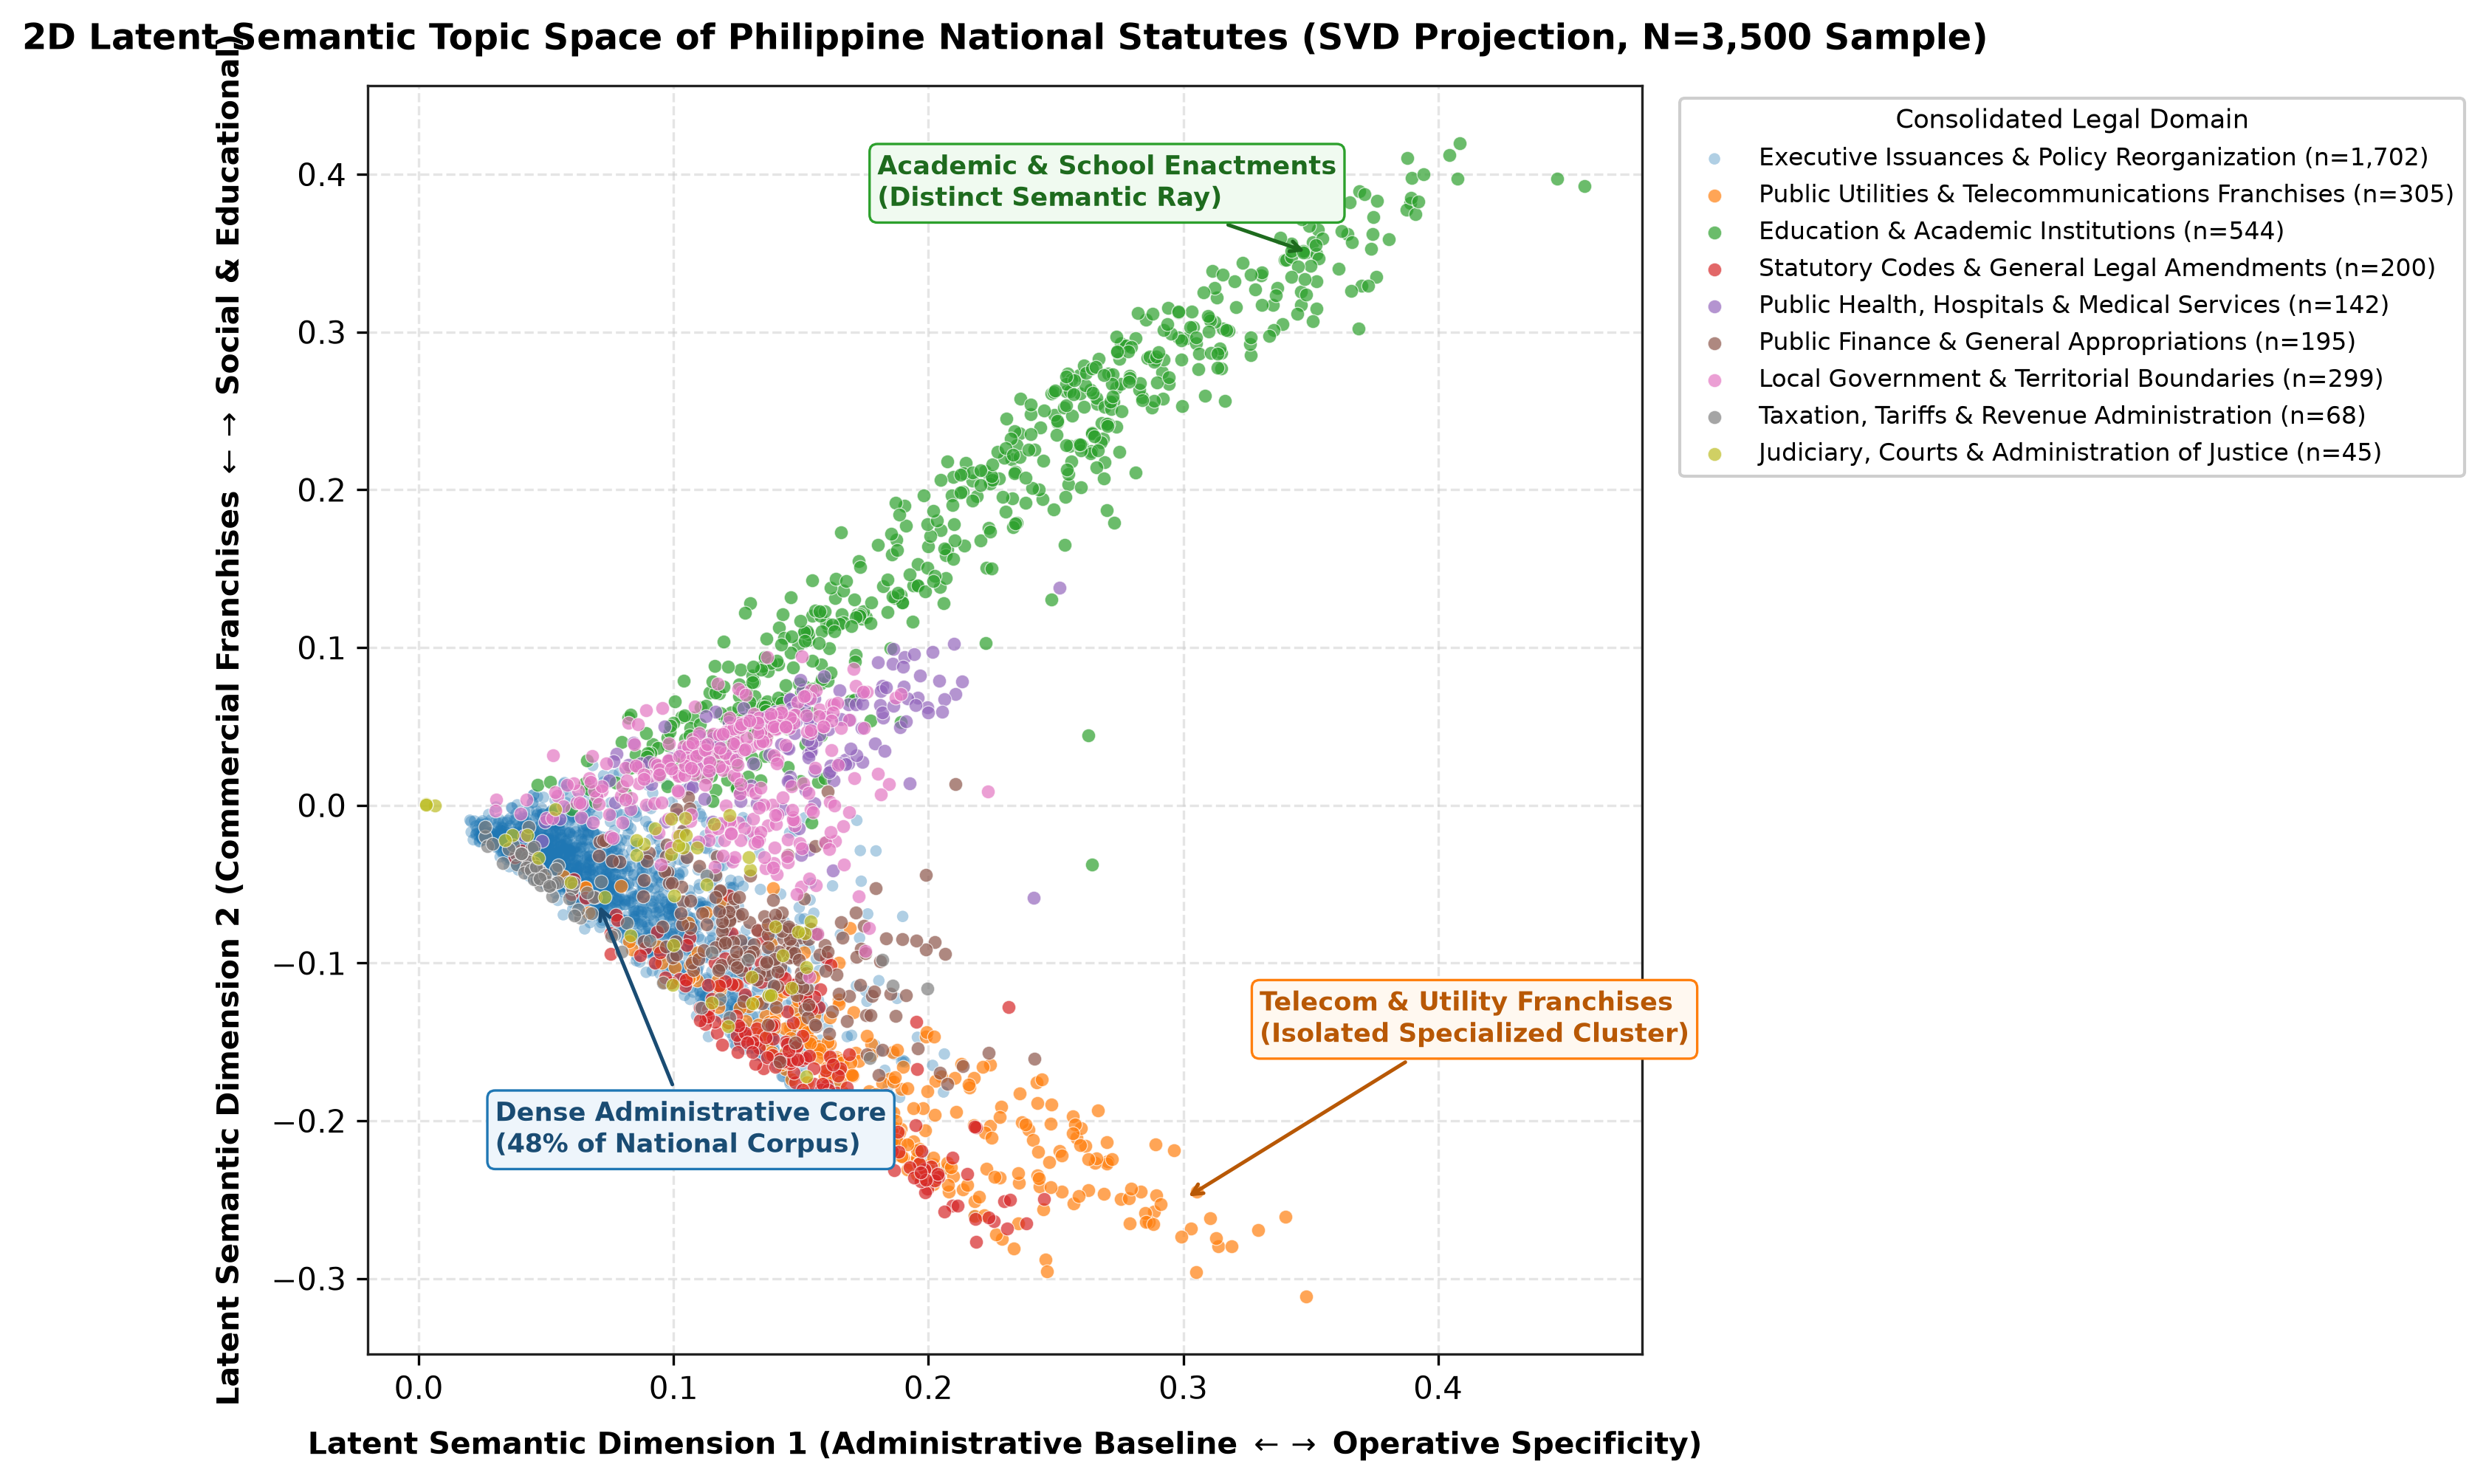
\includegraphics[width=0.92\linewidth]{figs/semantic_topic_landscape_2d.png}
            \caption{Two-Dimensional Latent Semantic Topic Space of the Philippine National Statutory Corpus (SVD Projection, $N = 3,500$ Representative Sample).}
            \label{fig:semantic_topic_landscape_2d}
        \end{figure}

        The two-dimensional semantic landscape reveals two distinct structural properties in Philippine statutory text. First, specialized regulatory domains project outward as distinct, isolated rays along the periphery of the vector space. Enactments establishing academic institutions and telecommunications franchises form tight, cohesive rays with minimal dispersion. In contrast, administrative issuances and executive orders cluster densely near the origin, comprising almost half of the entire archive. This dense central mass explains why unconstrained semantic searches frequently drift toward routine bureaucratic orders unless restrained by hierarchical safeguards.

        The coordinate axes reflect the two primary orthogonal directions of vocabulary variation discovered through singular value decomposition. The horizontal axis measures operative statutory specificity against general administrative phrasing, where higher positive values indicate detailed technical mandates rather than procedural orders. Conversely, the vertical axis captures functional divergence between social infrastructure such as public schools and commercial infrastructure such as telecommunications franchises. Although the dense cluster on the left appears visually compacted on a two-dimensional plane, the underlying MiniBatch $K$-Means clustering was performed in 64 dimensions where mathematical boundaries remain well-separated. Projecting 64 dimensions onto a flat plane inevitably collapses higher-order distinctions, yet this dense central mass visually demonstrates why unconstrained semantic retrieval suffers from search drift without domain filtering.

        To confirm that the mathematical clusters reflect substantive legal categories rather than shared administrative boilerplate, the proponents examined the most salient vocabulary terms discovered by the model. Words that appear frequently across all documents fail to differentiate legal topics, requiring class-based weightings to isolate subject matter. Figure~\ref{fig:top_keywords_per_domain} displays the top class-based TF-IDF ($c\text{-}TF\text{-}IDF$) keywords across all eight consolidated macro domains.

        \begin{figure}[!htbp]
            \centering
            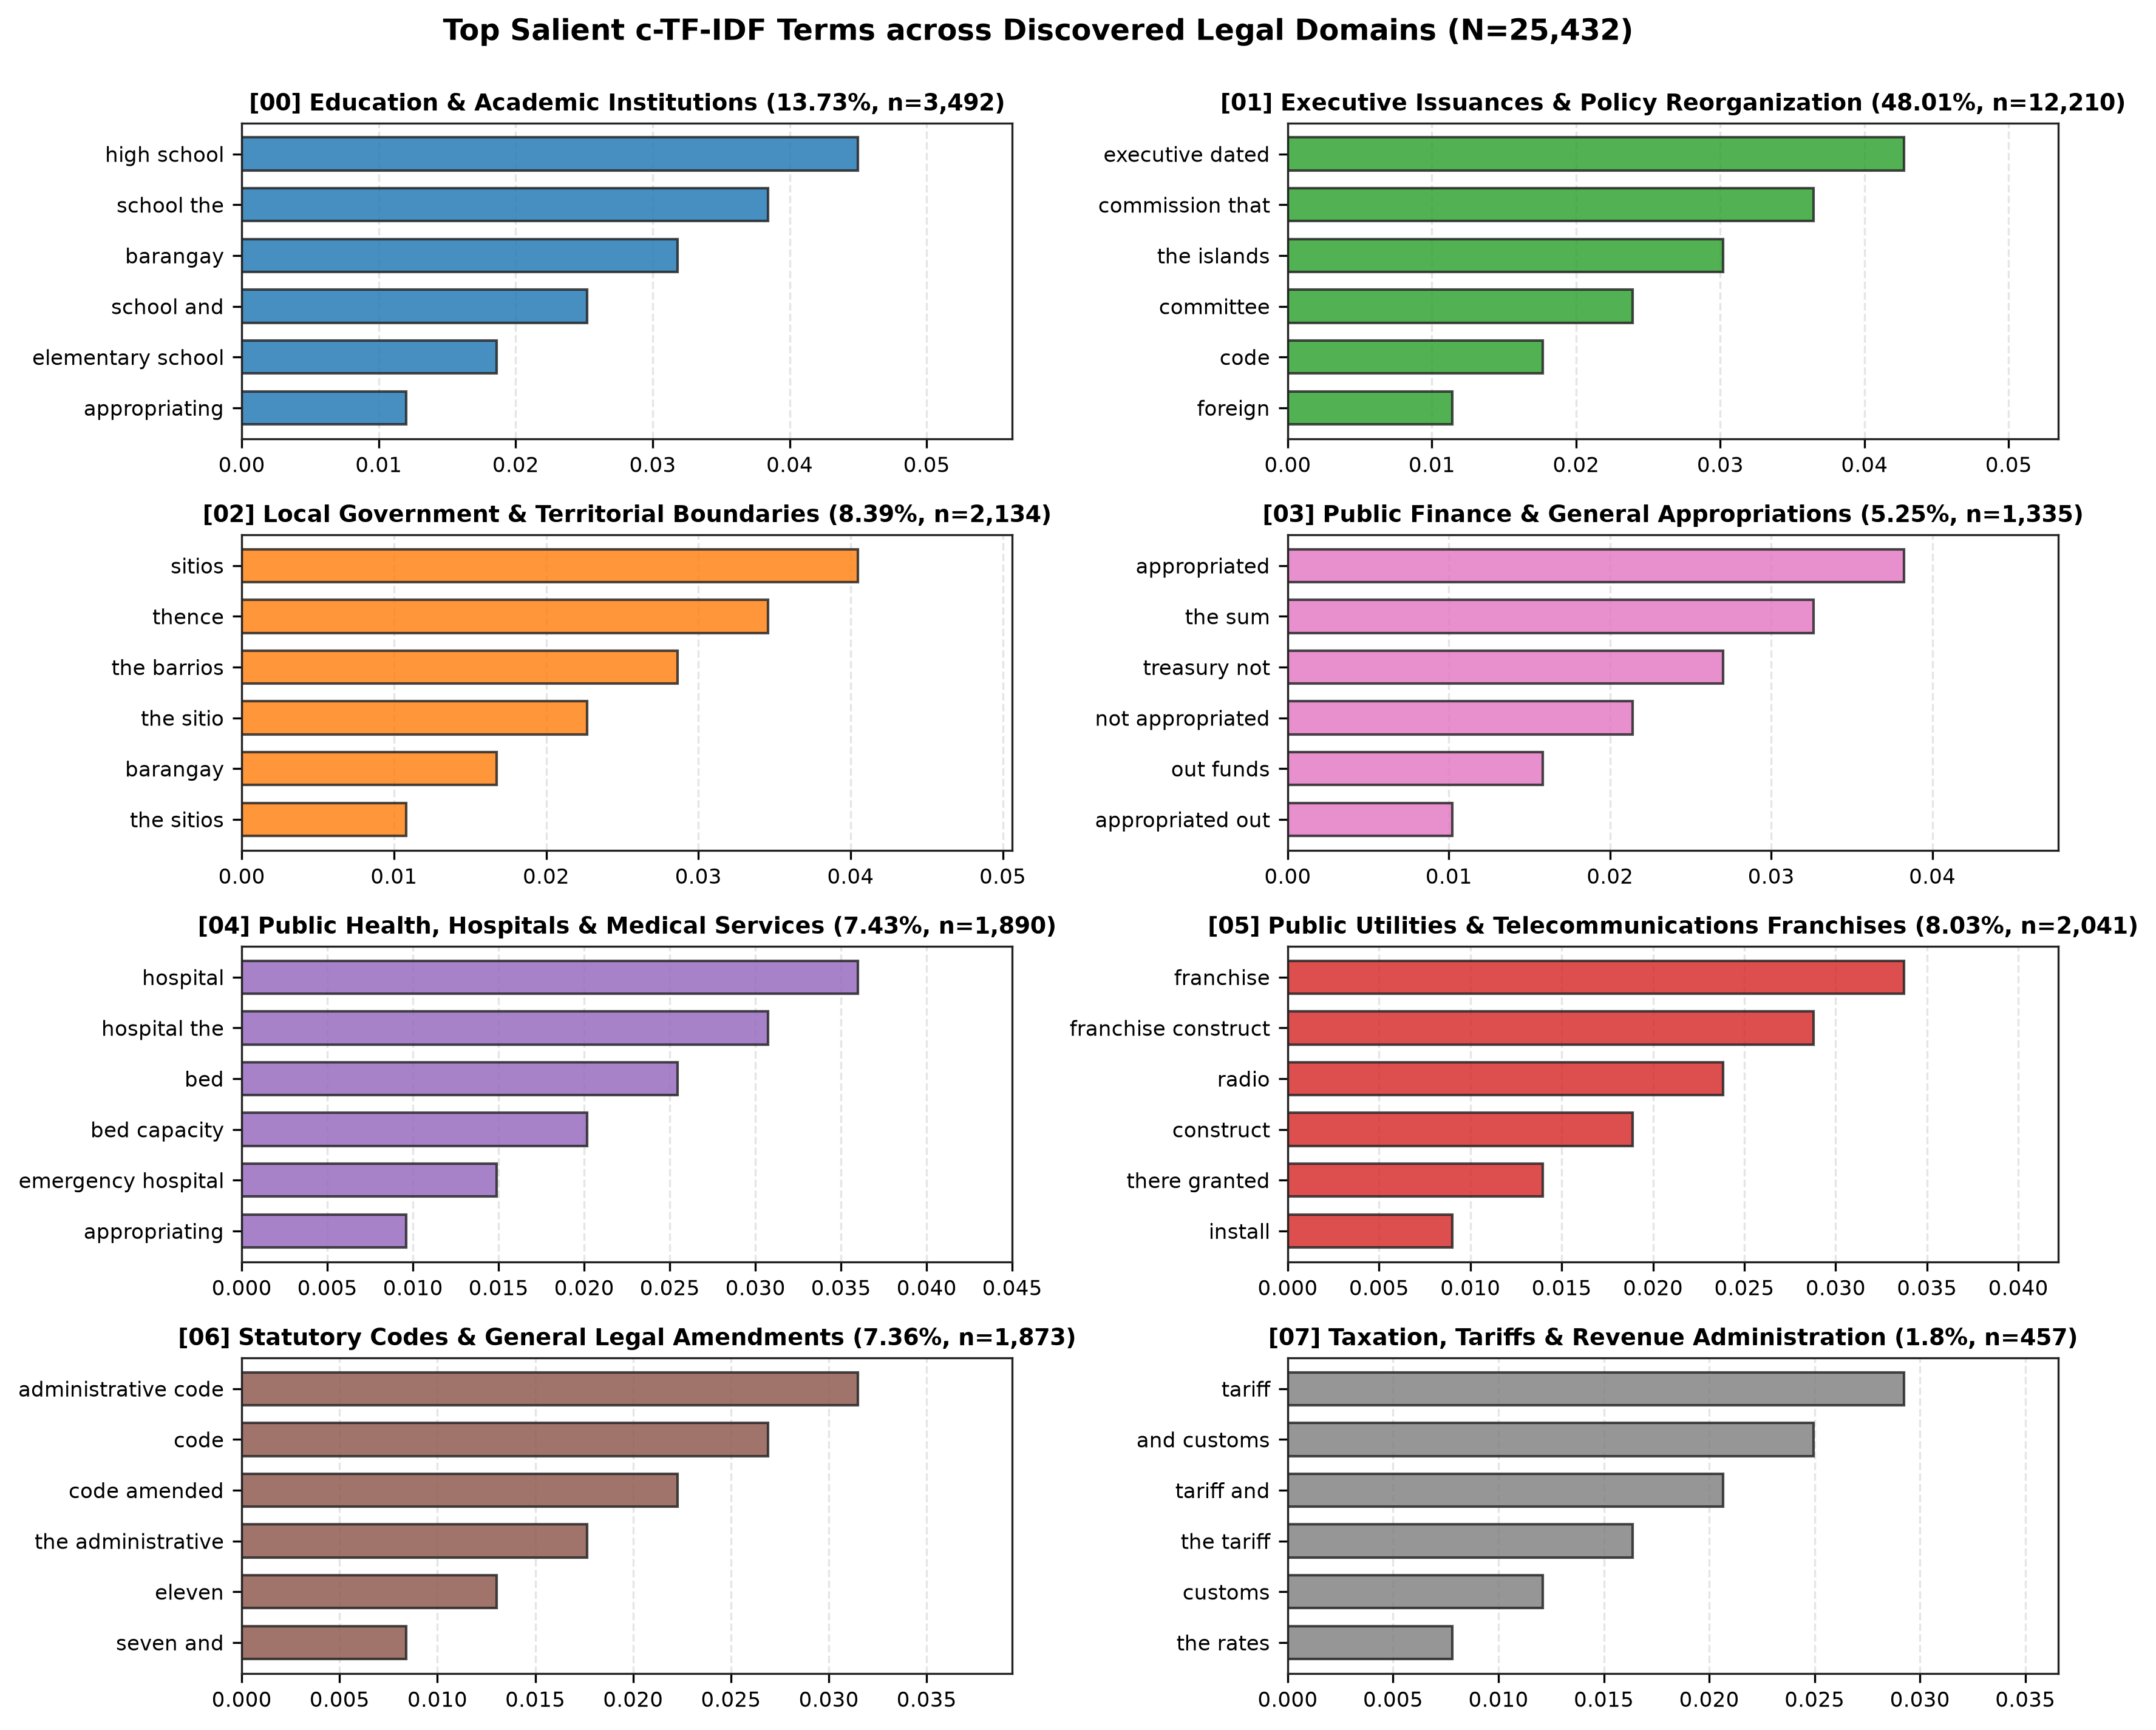
\includegraphics[width=0.78\linewidth]{figs/top_keywords_per_domain.png}
            \caption{Top Salient $c\text{-}TF\text{-}IDF$ Keyword Profiles across the Eight Consolidated Macro Legal Domains ($N = 25,432$).}
            \label{fig:top_keywords_per_domain}
        \end{figure}

        The vocabulary profiles confirm that each macro domain is defined by operative legal terminology unique to its statutory field. Specialized clusters such as public health are dominated by concrete institutional terms, including ``hospital,'' ``bed capacity,'' and ``medical center.'' Similarly, territorial boundary enactments display spatial cartographic markers such as ``sitio,'' ``barrio,'' and directional bearings. General administrative codes feature broader amendment verbs and statutory cross-references. These distinct vocabulary distributions confirm that the unsupervised clustering algorithm captures authentic legal subject matter across diverse legislative eras.

        To examine how individual lawmaking authorities contribute to these eight subject areas, the proponents mapped the six statutory instruments across the consolidated macro domains. In Philippine legislative history, different legal instruments serve distinct constitutional functions, ranging from broad congressional acts to presidential executive directives. Figure~\ref{fig:statute_source_domain_cross_allocation} presents this cross-allocation matrix, detailing both absolute enactment counts and percentage distributions for each statutory source. This cross-tabulation reveals an explicit division of legal responsibility across Philippine statutory instruments. Analyzing this allocation confirms that regulatory subjects concentrate within specific legislative formats rather than distributing evenly across the archive.

        \begin{figure}[!htbp]
            \centering
            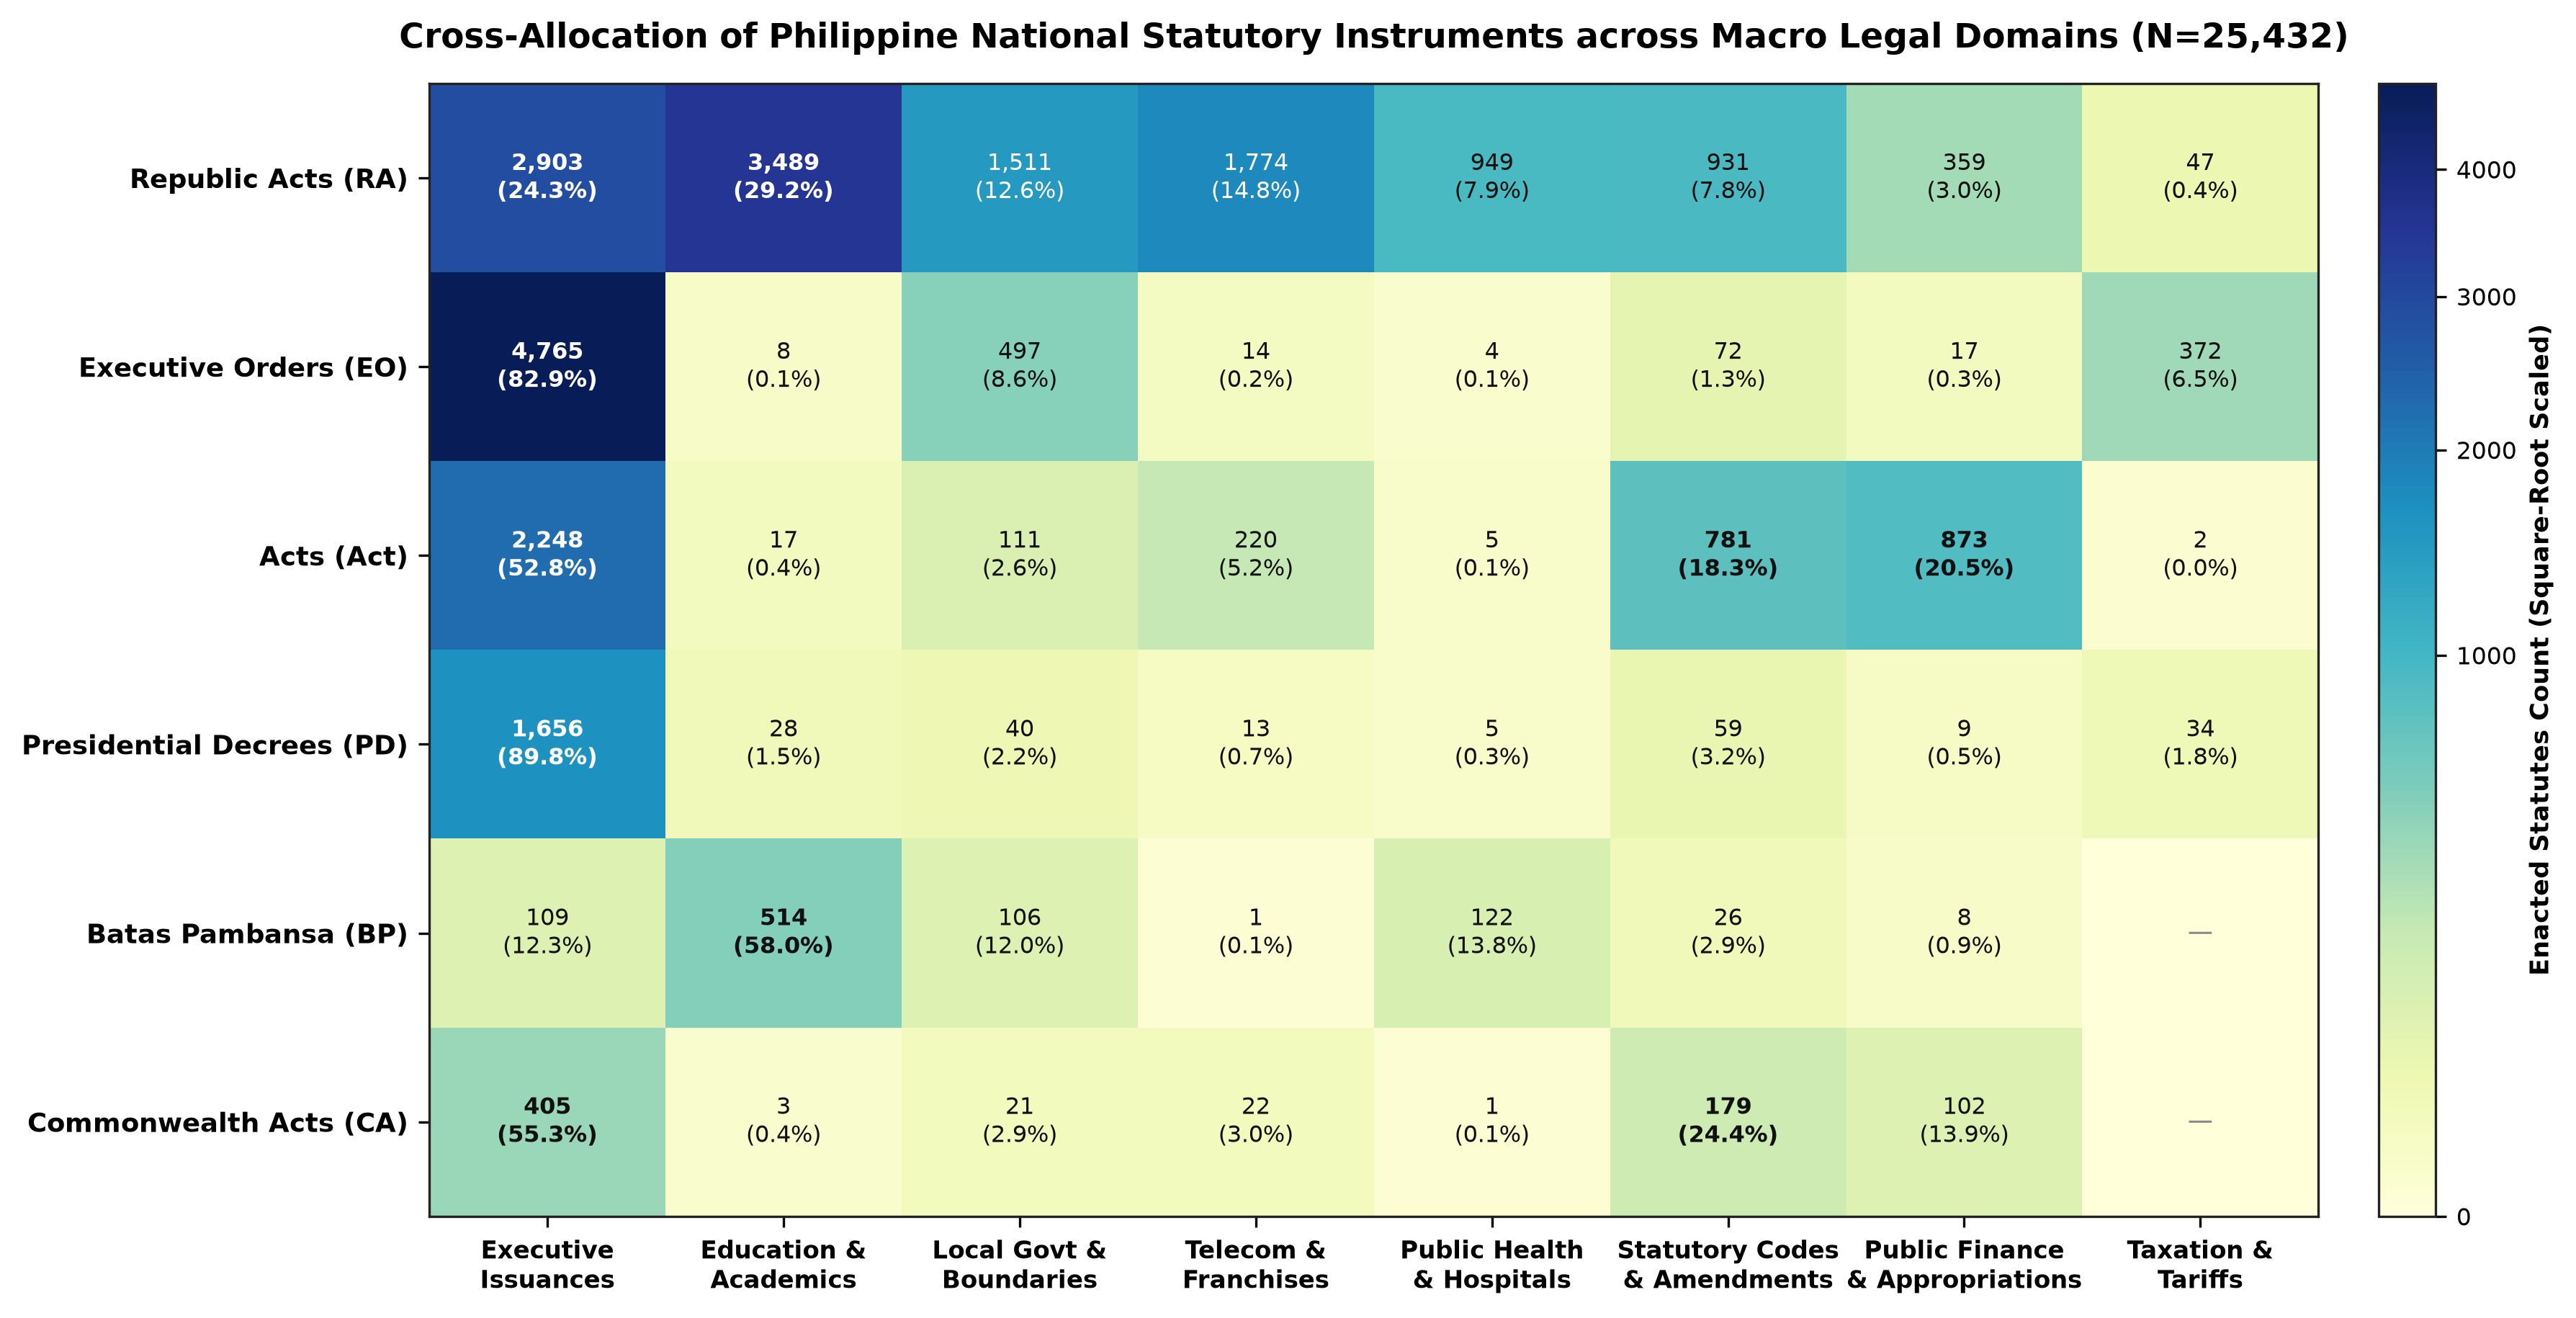
\includegraphics[width=0.80\linewidth]{figs/statute_source_domain_cross_allocation.png}
            \caption{Cross-Allocation Matrix of the Six National Statutory Instruments across the Eight Consolidated Macro Legal Domains ($N = 25,432$).}
            \label{fig:statute_source_domain_cross_allocation}
        \end{figure}

        The cross-allocation matrix reveals that congressional enactments and executive orders govern entirely separate legal spheres. Republic Acts account for nearly all specialized regulatory measures, containing 99.9\% of academic enactments and 86.9\% of telecommunications franchises. In contrast, Executive Orders concentrate heavily within administrative policy (82.9\%) and presidential tariff adjustments (81.4\%). Because municipal ordinances regulate local community behavior rather than internal executive operations, matching draft local clauses against executive orders produces high rates of irrelevant candidate retrievals. These empirical disparities validate using statutory source indicators and domain filters during Stage~1 retrieval to keep candidate shortlists focused on genuine regulatory mandates.

        To confirm that the topic pipeline discovered authentic legal boundaries rather than grouping surface vocabulary, the proponents evaluated the model using a stratified 80/20 train/test split. The 80/20 proportion follows the standard Pareto partition for large-scale legal collections exceeding 20,000 documents~\cite{aggarwal2012mining}, withholding 20\% of the corpus (5,087 statutes) to test generalizability on unseen enactments while training the model on the remaining 80\% (20,345 statutes). In statistical testing, an out-of-sample holdout of 5,087 legal texts provides high statistical power with a margin of error below $\pm 1.4\%$, making repetitive cross-validation computationally redundant as vocabulary frequencies and SVD components stabilize asymptotically at this volume. Stratified sampling preserves the natural historical proportions of the eight macro domains, ensuring that smaller regulatory categories like taxation (1.80\%, $N=457$) maintain adequate representation in the test set ($N_{\text{test}} \approx 91$) without class starvation. Table~\ref{tab:topic_holdout_validation} presents the out-of-sample performance scores, default random baselines, literature targets, and empirical verdicts across all evaluation criteria.

        \begin{table}[!htbp]
            \centering
            \footnotesize
            \renewcommand{\arraystretch}{0.95}
            \setlength{\tabcolsep}{3.5pt}
            \caption{Empirical Holdout Validation Metrics, Baseline Comparisons, and Literature Targets for the Topic Modeler ($N_{\text{train}} = 20,345, N_{\text{test}} = 5,087$)}
            \label{tab:topic_holdout_validation}
            \begin{tabularx}{\linewidth}{>{\RaggedRight}p{4.5cm}cc>{\Centering}p{2.3cm}>{\RaggedRight}X}
                \toprule
                \textbf{Validation Metric / Benchmark Test} & \textbf{Observed} & \shortstack[c]{\textbf{Default}\\\textbf{Baseline}} & \shortstack[c]{\textbf{Target}\\\textbf{Range}} & \textbf{Empirical Verdict} \\
                \midrule
                Out-of-Sample Supervised Accuracy & 97.37\% & 12.50\% & $\ge 85.0\%$ & Strong Generalization \\
                Out-of-Sample Macro F1-Score & 96.26\% & 12.50\% & $\ge 80.0\%$ & Balanced Discrimination \\
                Mean Test Cosine \mbox{Confidence} & 0.5508 & 0.1250 & $> 0.4000$ & Strong Dominant Probability \\
                High-Confidence Predictions ($\ge 0.50$) & 56.97\% & $< 20.0\%$ & $> 50.0\%$ & Clear Majority Cluster \\
                Holdout Cosine Silhouette Score & 0.1602 & $\le 0.0000$ & $0.1000\text{--}0.2000$ & Solid Text Separation \\
                Holdout Davies-Bouldin Index & 2.4496 & $> 4.0000$ & $2.0000\text{--}3.0000$ & Compact Cluster Scatter \\
                \midrule
                \multicolumn{5}{l}{\textbf{Explicit Statutory Title Probes} (\textit{Unambiguous Indicator Subsets, $N=1,259$})} \\
                \midrule
                Telecom Franchise Pattern & 97.8\% & 12.50\% & $> 90.0\%$ & High Precision ($N=360$) \\
                Hospital Bed Capacity \mbox{Pattern} & 96.6\% & 12.50\% & $> 90.0\%$ & High Precision ($N=203$) \\
                School Infrastructure \mbox{Pattern} & 92.2\% & 12.50\% & $> 90.0\%$ & High Precision ($N=645$) \\
                Judiciary \& Court Pattern & 72.5\% & 12.50\% & $> 70.0\%$ & Acceptable ($N=51$, embedded laws) \\
                \bottomrule
            \end{tabularx}
        \end{table}

        The supervised benchmark results confirm that the discovered macro domains generalize reliably to unseen legislation. In an eight-domain classification setting, the uniform proportional chance criterion established by Morrison~\cite{morrison1969interpretation} yields a default random baseline accuracy of only 12.50\% ($1/8$). In contrast, the validation classifier reached an out-of-sample accuracy of 97.37\% and a Macro F1-Score of 96.26\%, surpassing the 85.0\% target threshold typically expected for reliable document categorization~\cite{aggarwal2012mining}. To provide an external sanity check beyond learned cluster labels, the evaluation tested four explicit statutory title probes ($N=1,259$ total) where legislative intent is unmistakable from the statutory catchline. The model achieved 97.8\% precision on telecommunications franchises ($N=360$), 96.6\% on hospital bed capacity acts ($N=203$), and 92.2\% on school infrastructure laws ($N=645$). The lower precision on court reorganization acts (72.5\%, $N=51$) occurs because historical judicial reforms were frequently enacted as embedded chapters within general administrative codes rather than separate court charters.

        The probabilistic confidence metrics evaluate how decisively the model assigns unseen statutes to their respective legal domains. In an eight-domain distribution, equal uncertainty across all classes results in a default probability baseline of 0.1250 (12.50\%) under standard multinomial chance models~\cite{morrison1969interpretation}. Across all 5,087 holdout statutes, the model achieved a Mean Test Cosine Confidence of 0.5508 (55.08\%), exceeding the typical 0.4000 operational target and demonstrating that the top assigned category captured more than half of the total probability mass. Furthermore, 56.97\% of all unseen statutes were classified with high certainty ($\ge 0.50$ probability), well above the majority target threshold of 50.0\%. The remaining 43.03\% of statutes received confidence scores between 0.25 and 0.49 because Philippine legislation frequently addresses multiple regulatory areas within a single enactment. For example, general appropriations bills and administrative reorganizations distribute their probability across public infrastructure and local governance while still correctly assigning the dominant primary domain.

        The geometric clustering metrics evaluate whether the 64-dimensional SVD vector space forms well-separated and compact legal clusters. The holdout evaluation yielded a Cosine Silhouette Score of 0.1602 against the foundational baseline established by Rousseeuw~\cite{rousseeuw1987silhouettes}, where values near or below zero indicate overlapping, unseparated data points. While synthetic low-dimensional benchmarks often target silhouette scores above 0.50, text-mining literature demonstrates that high-dimensional document clustering rarely exceeds 0.20 due to shared vocabulary across legal topics~\cite{aggarwal2012mining}. In natural language processing, a positive silhouette score between 0.10 and 0.20 provides solid evidence of meaningful cluster cohesion and separation. Similarly, the model achieved a Davies-Bouldin Index of 2.4496, well within the target range of 2.0000 to 3.0000 formulated by Davies and Bouldin~\cite{davies1979cluster} and substantially below the diffuse clustering threshold of 4.0000. These geometric measurements prove that the topic model establishes stable, mathematically separated legal boundaries before documents are indexed for coarse retrieval.

        \subsubsection{Preprocessing and Chunking}
        To determine effective chunking boundaries, the proponents analyzed document and section lengths across the entire national statutory corpus ($N = 25,432$). Full national enactments span a wide spectrum of text lengths, ranging from brief presidential decrees to massive statutory codes containing hundreds of articles. In transformer-based natural language processing, text is segmented into subword units or ``tokens'' (where 1,000 tokens correspond to approximately 750 words in formal English legal text) and processed through self-attention mechanisms bounded by a fixed maximum sequence length (typically 512 tokens)~\cite{devlin2019bert}. Direct document-level matching causes severe context dilution because long enactments far exceed this 512-token sequence limit~\cite{wu2025aiir}. Dividing national legislation into natural section units aligns with legislative drafting structures where each section forms a self-contained legal rule. Figure~\ref{fig:statutory_length_disparity} illustrates the character length distribution of full statutes alongside the empirical token distributions and domain compliance rates across all 164,620 extracted section provisions.

        \begin{figure}[htbp]
            \centering
            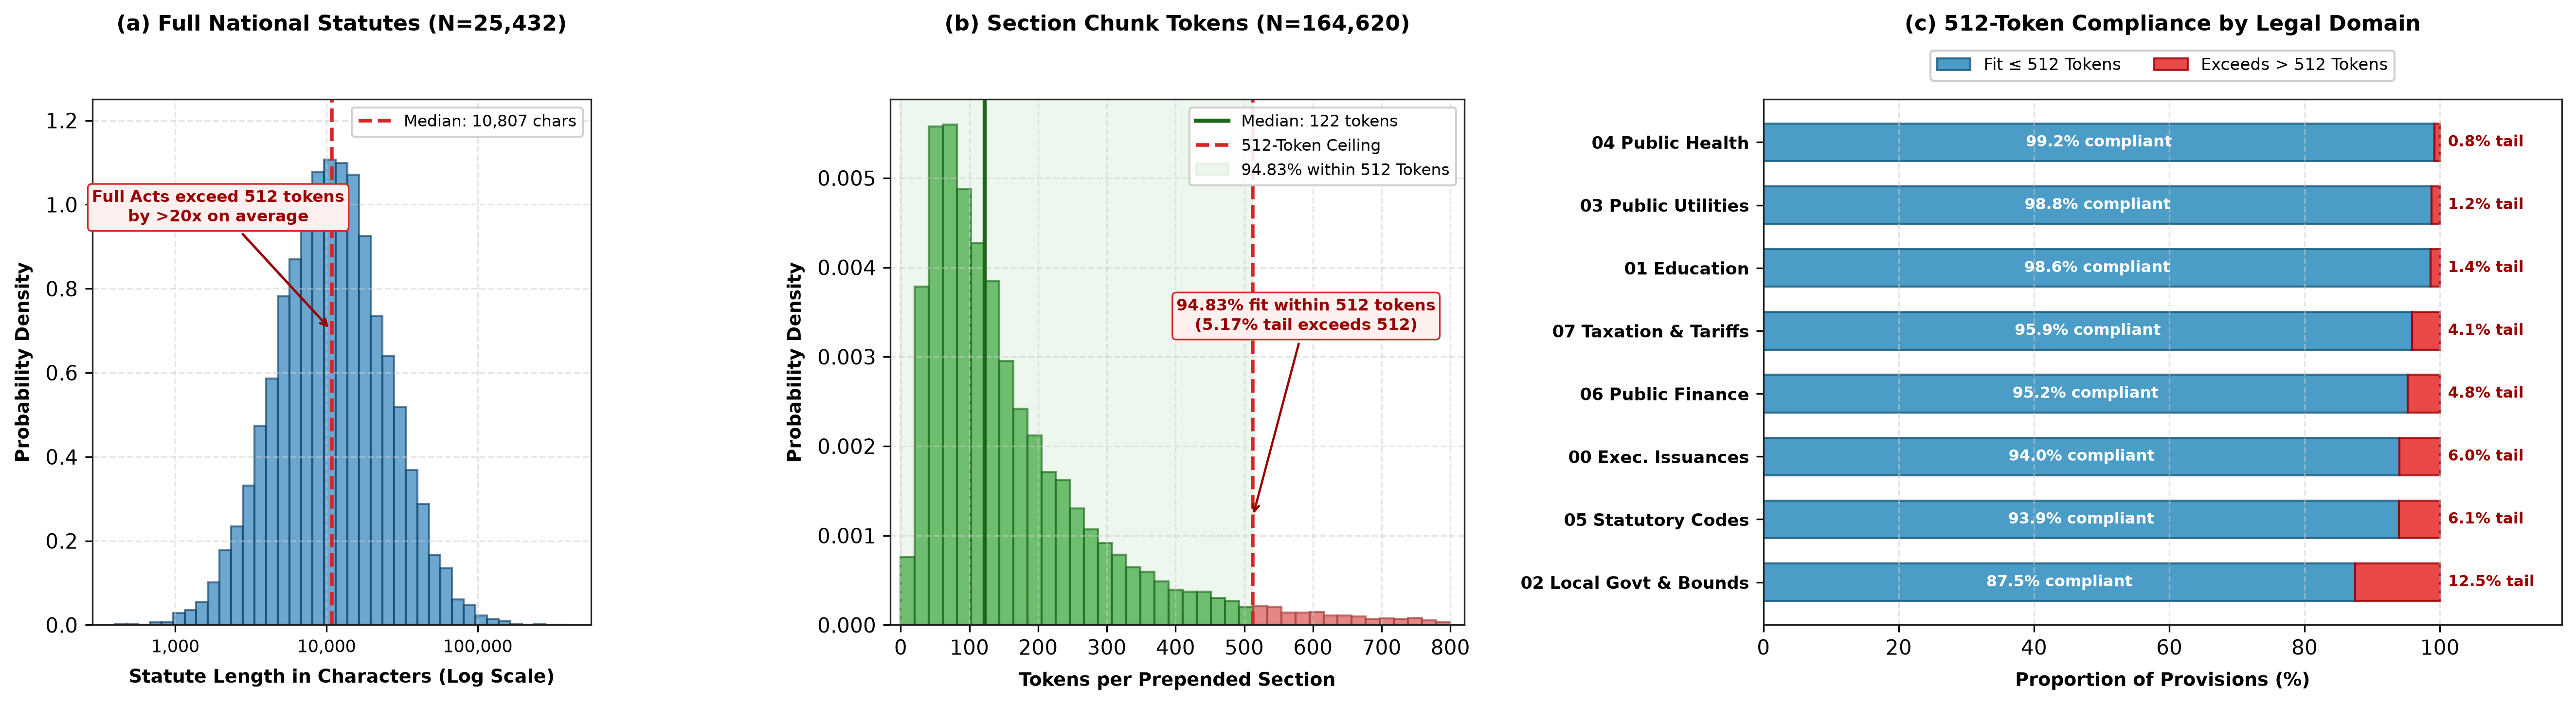
\includegraphics[width=0.98\linewidth]{figs/statutory_length_disparity.png}
            \caption{Document Length Distributions, Prepended Section Token Granularity, and 512-Token Compliance Rates across the Philippine National Statutory Corpus ($N = 25,432$ Statutes, $N = 164,620$ Sections).}
            \label{fig:statutory_length_disparity}
        \end{figure}

        The empirical distributions confirm that section-level chunking provides a practical input format for statutory retrieval. Across all 25,432 national statutes, full enactments exhibit a median length of 10,807 characters, with comprehensive codifications regularly exceeding one hundred thousand characters. In contrast, an empirical census of all 164,620 statutory sections reveals a median length of only 122.0 tokens after prepending the structural metadata header. Exactly 94.83\% of all prepended provisions (156,109 sections) fit completely within the 512-token attention window of standard transformer encoders. Segmenting legislation at natural section boundaries preserves complete legal rules while eliminating the need for arbitrary sliding windows that fragment statutory conditions.

        Examining token lengths across the eight macro legal domains explains how drafting styles differ between statutory subjects. Regulatory categories interact closely with municipal powers and demonstrate high compliance rates, led by Public Health (99.16\%), Public Utilities (98.78\%), Education (98.64\%), and Taxation (95.86\%). The only category with a noticeable exceedance tail is Local Government and Territorial Boundaries, where 12.54\% of sections exceed 512 tokens due to lengthy metes-and-bounds surveying descriptions. Across the entire national corpus, only 5.17\% of provisions exceed the 512-token threshold.

        To handle provisions in this 5.17\% tail without information loss under standard-context models, the pipeline implements a hierarchical overlapping sub-chunking fallback. Adapting the sliding window strategy formulated by Devlin et al.~\cite{devlin2019bert} for transformer sequence constraints, when an extracted statutory section exceeds a safety threshold of 448 tokens, the preprocessing module divides the section into overlapping sub-chunks using a window of $w = 384$ tokens and a stride of $s = 256$ tokens (128-token overlap). Capping the sub-chunk window at 384 tokens reserves a 64-token structural buffer within the 512-token ceiling to accommodate the prepended metadata header along with mandatory special tokens ($[CLS]$, $[SEP]$)~\cite{devlin2019bert}. Each sub-chunk preserves the prepended structural metadata header $\left[ \text{Statute Title}, \text{ Section } S_i\text{: Catchline} \right]$ to maintain institutional context. In Stage~1 retrieval, the parent provision embedding is computed by mean-pooling the sub-chunk vectors, capturing semantic concepts across all paragraphs. In Stage~2 inference, the Cross-Encoder evaluates each sub-chunk independently against the local ordinance hypothesis $h$, determining the provision-level conflict through max-pooling across sub-chunk contradiction probabilities:
        \[
            \hat{P}(\text{Contradiction} \mid p_i, h) = \max_{j} P\left(\text{Contradiction} \mid p_{i,j}, h\right)
        \]
        where $p_{i,j}$ denotes the $j$-th sub-chunk of statutory section $p_i$. This max-pooling aggregation ensures that an isolated prohibition or restrictive condition buried deep in a multi-paragraph section triggers the contradiction alert without being diluted by surrounding agreeable text.

        Alongside the sub-chunking fallback, the proponents evaluate ModernBERT as a long-context candidate architecture~\cite{warner2024modernbert, kadowaki2025modernbert}. By combining FlashAttention-2 with rotary positional embeddings, ModernBERT natively processes input sequences up to 8,192 tokens, completely bypassing the need for text segmentation. The researchers hypothesize that ModernBERT is uniquely valuable for this 5.17\% tail of lengthy codifications and boundary descriptions where sequence truncation could otherwise occur. However, for the 94.83\% majority of concise provisions with a median length of only 122 tokens, standard-context architectures such as DeBERTa-v3~\cite{he2023debertav3} and MiniLM~\cite{reimers2019sentencebert} may achieve sharper semantic discrimination and faster inference on local office workstations. Evaluating both model families directly tests whether native long-context support outperforms compact, standard-window models across Philippine statutory texts.

        After establishing the need for granular text units, the preprocessing pipeline cleans local ordinance texts and national statutory provisions. Custom regular expressions find and remove repetitive introductory preamble paragraphs and official signature blocks from city ordinances. Unlike ordinary documents, legal acts follow an organized structure divided into numbered chapters and sections. The researchers divide statutes at the section level rather than using fixed word-count windows~\cite{wu2025aiir}. In Philippine legal drafting, each section acts as a complete rule, stating a main legal command along with its specific conditions and exceptions.

        Splitting text by an arbitrary word count can easily cut a legal rule in half, separating exceptions from the main requirement. When sub-clauses are separated this way, they lose the context of who must follow or enforce the rule. To preserve complete legal meaning, the preprocessing pipeline adds a structural metadata header to each chunk before saving it in the vector database. Every extracted statutory section begins with a header containing the statute title, section number, and section title:
        \[
            \mathbf{x}_{\text{chunk}} = \left[ \text{Statute Title}, \text{ Section } S_i\text{: Catchline} \right] \mathbin{\Vert} \mathbf{t}_{\text{verbatim}}
        \]
        where $\mathbf{t}_{\text{verbatim}}$ denotes the exact text extracted from Lawphil, and $\mathbin{\Vert}$ represents text joining. This prefix helps the Stage~2 Cross-Encoder immediately recognize the governing authority and official context of the provision.

        The practical need for these headers is shown by sections within composite legal codes. In Republic Act No.~7160, Section~447 sets penalty limits for municipalities, while Section~458 sets distinct penalty limits for city councils. Without adding the section title and number, downstream Cross-Encoders can confuse different levels of local government and misjudge municipal powers. Adding the structural metadata ensures that the model evaluates each legal clause under its correct administrative level. As a result, the vector embeddings retain both the exact wording of the clause and its broader statutory context.

        \subsubsection{Exception Handling}
        A key challenge in conflict detection is telling the difference between a real legal clash and an authorized legal exception. In regulatory laws, general prohibitions and permitted exceptions often appear in the same section using conditional phrasing. Because statutory sections average between 200 and 500 words, an entire section fits within the 512-token input limit of candidate Cross-Encoders. The model's attention mechanism can read the general rule and its internal exceptions together, preventing the system from incorrectly flagging valid local exceptions as conflicts. This structure helps keep the legal relationship between general rules and local exceptions clear.

        When a general ban and an exception appear in separate sections of a statute, the pipeline relies on the two-stage search process. An ordinance clause that drafts an authorized exception often uses words that match both the general ban and the exception section. The Stage~1 hybrid retriever searches both keyword and vector indexes, helping bring both candidate sections into the top-$k$ candidate shortlist. Stage~2 then evaluates each candidate section individually, allowing the system to identify the authorizing provision and confirm that the local rule is valid. This multiple-candidate review prevents premature conflict warnings on complex laws that place their exceptions in separate sections.

        In Philippine statutory construction, related enactments and provisions governing the same subject matter must be interpreted together as a harmonious whole under the doctrine of \textit{in pari materia}~\cite{agpalo2009statutory}. Under this established legal rule, an isolated subsection cannot be understood in a vacuum without the overarching context of its governing section and related statutory exemptions. If an ordinance draft relies on an authorized statutory exemption, evaluating a specific clause like a penalty rule without retrieving the parent exception can trigger an incorrect conflict warning. The system addresses this challenge by prepending hierarchical catchlines to granular sub-clauses during preprocessing and using hybrid retrieval to pull both general bans and specific exception clauses into the candidate shortlist. The Cross-Encoder can then evaluate the draft against the authorizing exception clause and assign an Entailment classification, confirming that the local measure operates within valid legislative authority.

        \subsection{Ground Truth Benchmark Construction}
Evaluating candidate Cross-Encoder models in Stage~2 requires a high-quality ground truth dataset. Unlike the broad search phase, the Natural Language Inference (NLI) model needs expert-verified examples to train and measure its classification accuracy. Because standard NLP benchmarks do not include Philippine local laws, a custom dataset had to be created for Davao City. This curated collection provides a clear benchmark for identifying legal conflicts between draft local ordinances and national statutes. In this way, the ground truth dataset connects basic language processing with real-world legal analysis.

\subsubsection{Span Pairing}
        \label{sec:span_pairing}
        To construct a representative ground truth benchmark, candidate statutory premises must reflect the full breadth of Philippine national law. During the exploratory phase of this research, the proponents conducted preliminary machine learning experiments on the national statutes, uncovering severe class imbalances and repetitive drafting formulas across historical eras. These exploratory findings directly informed the consolidated topic modeling architecture detailed in Section~\ref{sec:domain_categorization}, which organizes the corpus into eight validated Macro Legal Domains such as local governance, public health, and taxation. The proponents then sampled national statutory sections across these eight domains to establish the fixed premises for the evaluation benchmark. To evaluate multi-sentence legal commands without breaking internal qualifications, the pipeline uses Asymmetric Span-Level Pairing, coupling each statutory premise with a multi-sentence ordinance hypothesis block~\cite{yin2021docnli}. This asymmetric structure ($1\text{ premise vs } N\text{ hypothesis sentences}$) ensures that local exceptions, cross-references, and penalty conditions are evaluated together against the national law~\cite{koreeda2021contract}.

        To make the evaluation as realistic as possible, the drafted test sentences closely mirror the writing style of Davao City ordinances. The proponents analyzed municipal laws enacted between 2021 and 2025 to identify standard drafting phrases, administrative office names, and structural penalty clauses following the official drafting conventions of the Department of the Interior and Local Government (DILG)~\cite{dilg2022drafting}. Each drafted clause uses standard enacting syntax, such as: ``\textit{SECTION X. [TITLE]. --- It shall be unlawful for any person, natural or juridical, within the territorial jurisdiction of Davao City, to...}'' The draft sentences also name real local enforcement bodies, such as the City Transport and Traffic Management Office (CTTMO), the City Health Office (CHO), the City Environment and Natural Resources Office (CENRO), and the Business Bureau of Davao City. Operational units such as the Anti-Vices Task Force (AVTF) and the Davao City Police Office (DCPO) are also included to reflect genuine local enforcement.

        The synthetic ordinance clauses are also linked to real administrative districts in Davao City. Draft rules specify geographic areas from urban centers like Poblacion and Talomo to suburban districts like Buhangin and Toril. Local offices such as the City Disaster Risk Reduction and Management Office (CDRRMO) and the City Social Welfare and Development Office (CSWDO) are included to match actual city administration. This realistic drafting prevents evaluators from reviewing artificial example sentences that differ from real legal texts. As a result, the 15 Sangguniang Panlungsod legal researchers evaluate draft provisions that look like real measures introduced on First Reading.

        The proponents deliberately utilized expert-curated, domain-grounded hypothesis construction based on authentic local templates rather than unconstrained synthetic generation via large language models. Recent evaluations by Gururangan et al.~\cite{gururangan2018annotation} and Poliak et al.~\cite{poliak2018hypothesis} demonstrated that automated or crowd-generated NLI hypotheses frequently introduce severe ``annotation artifacts''—systematic lexical cues such as negation markers (``not'', ``never'') that allow neural models to cheat and predict contradictions without genuinely reading the statutory premise. In specialized legal domains, authoritative benchmarks such as SARA (tax law)~\cite{holzenberger2020a}, DocNLI~\cite{yin2021docnli}, and Clash-of-Leges~\cite{italiani2026clash} establish that rigorous evaluation requires domain-grounded hypotheses reflecting authentic legislative syntax, ensuring models are tested on genuine statutory reasoning rather than superficial generation heuristics.

        While the system uses multi-sentence spans to understand local context, it does not attempt cross-document multi-hop reasoning (detecting conflicts that appear only by combining two or more separate national laws). Resolving dependencies across multiple separate laws is an active research challenge in natural language inference. Current systems that attempt this require either complex knowledge graphs~\cite{lu2023multi} or very large generative language models~\cite{shen2025hopweaver}. Running those multi-premise models would exceed the consumer-grade hardware limits set for local government deployment. For this reason, the ground truth benchmark and the inference system focus strictly on single-premise evaluations.

        \subsubsection{Class Balancing and Adversarial Injection}
        In standard machine learning on tabular data, researchers often handle uneven classes using methods like the Synthetic Minority Over-sampling Technique (SMOTE)~\cite{chawla2002smote}. However, the proponents avoid continuous vector oversampling for this legal text pipeline. SMOTE creates artificial examples by interpolating between numerical feature vectors ($x_{\text{new}} = x_i + \lambda(x_{zi} - x_i)$). In high-dimensional language models representing discrete words, averaging or blending token vectors creates artificial representations that confuse attention layers and carry no real legal meaning. Simple word replacement also fails with legal texts because statutory words have exact legal definitions; for example, swapping mandatory words like ``shall'' with permissive words like ``may'' fundamentally changes a legal duty.

        To build a balanced, reliable Ground Truth dataset, the researchers combined historical legal records with expert-guided text adjustments. First, the researchers gathered documented legal clashes from local government records, including mayoral veto messages, repealed ordinances, and explicit statutory amendments~\cite{italiani2026clash}. Second, following the evaluation methods of Koreeda and Manning~\cite{koreeda2021contract} and Nie et al.~\cite{nie2020anli}, legal annotators introduced conflicting rules into real statutory provisions. Annotators reversed permissions, changed numerical zoning limits, and added conflicting penalties into ordinance clauses. This expert-guided process produced a balanced distribution across the Entailment, Neutral, and Contradiction classes in the 350 Ground Truth pairs, preventing class imbalance without creating unnatural legal phrasing.

    \subsubsection{Jurisprudential Difficulty Tiers}
        Building an effective evaluation benchmark requires pairs with varying levels of difficulty. If all contradiction examples were simple penalty ceiling violations or obvious word swaps, models could score well by memorizing shallow keyword patterns~\cite{mccoy2019right}. To construct a rigorous evaluation suite, the proponents adapted the difficulty tiering methodology established by Koreeda and Manning in the ContractNLI benchmark~\cite{koreeda2021contract}. This approach is supported by the behavioral stress-testing frameworks of Ribeiro et al.~\cite{ribeiro2020beyond} and Naik et al.~\cite{naik2018stress}, which separate surface competence tests from semantic challenge sets. Furthermore, the 30\% Tier~1, 40\% Tier~2, and 30\% Tier~3 quota follows the adversarial challenge partitioning established in benchmark engineering literature, such as SQuAD~2.0~\cite{rajpurkar2018know}, FEVER~\cite{thorne2018fever}, and ANLI~\cite{nie2020anli}. These foundational benchmarks establish that maintaining an adversarial challenge quota of 30\% to 40\% is optimal to prevent models from exploiting superficial lexical artifacts while preserving sufficient representation of standard rule-based compliance. Table~\ref{tab:conflict_difficulty_tiers} outlines the stratified difficulty tiers, legal conflict mechanisms, and representative examples for the 350-pair benchmark.

        \begin{table}[htbp]
            \centering
            \footnotesize
            \setlength{\tabcolsep}{4pt}
            \caption{Stratified Jurisprudential Difficulty Tiers for the 350-Pair Ground Truth Evaluation Benchmark}
            \label{tab:conflict_difficulty_tiers}
            \begin{tabularx}{\linewidth}{>{\RaggedRight}p{3.4cm}>{\centering\arraybackslash}p{1.4cm}>{\RaggedRight}X>{\RaggedRight}p{4.5cm}}
                \toprule
                \textbf{Difficulty Tier} & \textbf{Target Share} & \textbf{Legal Conflict Mechanism} & \textbf{Representative Statutory Example} \\
                \midrule
                \textbf{Tier 1: Surface \& Quantitative} & 30\% & Direct penalty ceiling violations and explicit changes in mandatory words (\textit{shall} converted to \textit{may}). & Local draft imposes a PHP~15,000 fine for traffic obstruction when RA 7160 Sec. 458 caps city penalties at PHP~5,000. \\
                \addlinespace[3pt]
                \textbf{Tier 2: Preemption \& Carve-Outs} & 40\% & Exceeding local regulatory powers under \textit{Magtajas}, and blanket local bans that omit statutory exceptions. & Draft ordinance enacts a total ban on commercial freight transit without exempting national agricultural and medical logistics. \\
                \addlinespace[3pt]
                \textbf{Tier 3: Latent \& Paraphrastic} & 30\% & Subtle conflicts where the draft redefines statutory terms or creates incompatible rules without using the exact statutory words. & Draft anti-vagrancy ordinance assigns apprehended minors to detention cells, violating non-custodial diversion under RA 9344 without citing the law. \\
                \bottomrule
            \end{tabularx}
        \end{table}

        The three difficulty tiers map directly to established Philippine municipal preemption doctrines and linguistic challenge categories, reflecting the jurisprudential distinction between rule-based and value-based normative conflicts formulated by Sartor~\cite{sartor2005legal} and Bench-Capon and Sartor~\cite{benchcapon2003theory}. Tier~1 evaluates surface and quantitative preemption, reflecting direct penalty ceiling violations under Section~458 of Republic Act No.~7160 and explicit modal verb clashes (\textit{shall} versus \textit{may}). Tier~2 adapts the ``negation by exception'' category from Koreeda and Manning~\cite{koreeda2021contract}, evaluating unhonored statutory exemptions and local overreach under \textit{Magtajas v. Pryce Properties}~\cite{scp1994magtajasvpryce} and \textit{City of Manila v. Laguio, Jr.}~\cite{scp2005manilavlaguio}. Tier~3 evaluates latent and paraphrastic contradictions, testing whether the model detects substantive statutory friction when a draft redefines terms without sharing exact statutory words. Allocating the benchmark into 30\% Tier~1, 40\% Tier~2, and 30\% Tier~3 establishes an adversarial quota that reflects real-world committee reviews while preventing models from exploiting simple lexical heuristics~\cite{mccoy2019right}.

        Grounding Tier~3 contradictions in legal doctrine ensures that models are evaluated on genuine language understanding rather than keyword presence. Under established Supreme Court rulings, a local council cannot enact indirect prohibitions that take away rights protected by national statutes~\cite{scp1994magtajasvpryce, scp2005manilavlaguio}. To enforce this distinction during testing, the proponents verified that all 104 Tier~3 draft sentences contain zero numbers or monetary amounts. Without explicit numerical clues, the Cross-Encoder must evaluate the underlying legal meaning of the text, such as recognizing when an anti-vagrancy draft detains minors in violation of Republic Act No.~9344. This design ensures that the benchmark provides an authentic diagnostic test of semantic preemption for the subsequent analysis in Chapter~4.

        \subsubsection{Annotation Workflow}
        Classifying the sampled text pairs requires domain-specific legal training to ensure authentic and reliable labels. The Davao City Sangguniang Panlungsod currently comprises 24 elected councilors across the city's three legislative districts, supported by a professional staff of approximately 48 active legal researchers~\cite{cortez2025leadership}. In the initial administrative correspondence transmitted to the Sangguniang Panlungsod Secretariat alongside the Legal Annotation Guidebook, the proponents formally requested a cohort of 15 volunteer legal researchers. Unlike general NLP tasks that rely on open crowdsourcing, legal natural language inference requires formal statutory interpretation skills to prevent superficial keyword matching~\cite{snow2008cheap, zheng2021when}. The recruited legal researchers review local ordinances as their regular professional duty, providing the necessary institutional competence for building a dependable gold standard~\cite{chalkidis2022lexglue}.

        To establish an objective and transparent panel structure, the proponents gathered baseline qualifications during the initial intake communication. The intake request systematically recorded two key criteria from each volunteer: highest educational attainment and total years of professional experience in legislative drafting. Using these reported credentials, the 15 researchers were organized into five balanced sub-panels of three members each ($k = 3$). Within each three-member sub-panel, the evaluator possessing the highest educational attainment and the longest drafting tenure was designated as that panel's Senior Annotator. The proponents then communicated these panel assignments and Senior Annotator designations in a follow-up confirmation email to establish operational readiness before annotation began.

        Following the consensus guidelines adapted from Ablazo~\cite{ablazo2019designing}, a label is accepted into the final Ground Truth if at least two of the three reviewers in a sub-panel agree. In cases where all three reviewers select different categories, resulting in a three-way split with no majority, the pair is referred to that panel's designated Senior Annotator for binding qualitative adjudication~\cite{gao2022hierarchical, artstein2008inter}. The Senior Annotator reviews the pair against the standardized codebook to resolve whether the split arose from statutory ambiguity or an overlooked proviso. This hierarchical adjudication step ensures that every item in the 350-pair benchmark reaches an authoritative label while preserving the initial independent ratings for calculating Fleiss' Kappa ($\kappa$). Maintaining this structured division between initial independent scoring and expert tie-breaking guarantees both statistical validity and qualitative consistency across the dataset.

        \subsubsection{Annotation Codebook}
        To help the 15 legal researchers apply consistent criteria, the proponents developed a standardized Legal Annotation Codebook. Adapting principles from Koreeda and Manning~\cite{koreeda2021contract} and Italiani et al.~\cite{italiani2026clash}, the codebook turns the three-class NLI framework into clear legal decision rules. Each evaluated pair consists of a single national statute section as the premise and a multi-sentence municipal ordinance clause as the hypothesis. Annotators assign one of three labels: Contradiction, Entailment, or Neutral. Table~\ref{tab:annotation_codebook} summarizes the working definitions, legal triggers, and example patterns used in the annotation guidelines.

        \begin{table}[htbp]
            \centering
            \footnotesize
            \setlength{\tabcolsep}{4pt}
            \caption{Sangguniang Panlungsod Ground Truth Legal Annotation Codebook and Decision Rules}
            \label{tab:annotation_codebook}
            \begin{tabularx}{\linewidth}{>{\RaggedRight\arraybackslash}p{2.4cm}>{\RaggedRight\arraybackslash}p{4.0cm}>{\RaggedRight\arraybackslash}X>{\RaggedRight\arraybackslash}p{4.0cm}}
                \toprule
                \textbf{Logical State} & \textbf{Operational Legal Definition} & \textbf{Primary Legal and Structural Triggers} & \textbf{Representative Statutory Pattern} \\
                \midrule
                \textbf{Contradiction} & The municipal ordinance prohibits what national statute permits, permits what statute prohibits, or exceeds statutory ceilings~\cite{scp1994magtajasvpryce}. & Clashes in mandatory words (\textit{shall} vs. \textit{may}); penalty limit violations (RA 7160 Sec. 458); territorial or franchise preemption. & National statute caps ordinance fines at PHP~5,000; draft ordinance mandates a PHP~15,000 penalty. \\
                \addlinespace[3pt]
                \textbf{Entailment} & The municipal ordinance directly executes, complies with, or derives its regulatory authority from the national premise without adding conflicting mandates. & Compliant devolved implementation; literal statutory adoption; regulatory enforcement within prescribed legislative boundaries. & Local draft establishes a municipal health board strictly adhering to the composition mandated by RA 7160. \\
                \addlinespace[3pt]
                \textbf{Neutral} & The national statute and municipal ordinance address the same broad legal domain, but govern independent obligations without mutual conflict or derivation. & Shared topic without direct legal clash; complementary administrative scopes; distinct non-overlapping legal subjects. & National statute establishes hospital licensing standards; local draft regulates municipal market sanitary permits. \\
                \bottomrule
            \end{tabularx}
        \end{table}

        The decision rules for Contradiction directly apply the consistency test established in the Magtajas Doctrine~\cite{scp1994magtajasvpryce}. Because local governments have delegated rather than unlimited legislative powers under Republic Act No.~7160~\cite{philgov1991ra7160}, any local draft that exceeds national statutory limits is legally invalid (*ultra vires*). Annotators look for shifts in mandatory language, such as turning a strict command (``shall'') into an optional choice (``may''), or removing an exemption that national law protects. In the test samples, numerical rules are audited against national limits, including tax caps and penalty ceilings. These criteria ensure that conflict warnings highlight actual legal problems rather than minor wording choices.

        The guidelines follow a structured consensus process to resolve disagreements among the three panel reviewers. When two or three reviewers agree, the majority label is accepted directly into the benchmark. In cases where all three reviewers select different categories, the item is referred to the sub-panel's designated Senior Annotator for final qualitative review~\cite{gao2022hierarchical}. The Senior Annotator reviews the evaluators' optional notes against the codebook to determine whether the difference came from subtle statutory phrasing or an overlooked exception. This review step ensures that every item in the 350-pair Ground Truth reaches an authoritative label while preserving the original votes to calculate Fleiss' Kappa.

        To illustrate the structure of the evaluated instances, Listing~\ref{lst:ground_truth_pair} presents an authentic sample record (Pair ID: \texttt{GT-001}) from the 350-pair Ground Truth benchmark dataset, showcasing the paired national statutory premise, proposed municipal hypothesis, gold conflict label, and expert legal rationale.

        \begin{lstlisting}[language=Python, caption={Sample Evaluation Pair from the Ground Truth Benchmark Dataset}, label={lst:ground_truth_pair}]
# Authentic Evaluation Pair GT-001 from data/ground_truth_350.jsonl
benchmark_pair = {
    "pair_id": "GT-001",
    "macro_domain": "Executive Issuances & Policy Reorganization",
    "difficulty_tier": "Tier 1: Surface & Quantitative",
    "national_premise": {
        "statute_title": "Republic Act No. 7581 (The Price Act)",
        "citation": "Section 6",
        "statutory_text": (
            "Section 6. Automatic Price Control. - Unless otherwise declared by the "
            "President, prices of basic necessities in an area shall automatically be "
            "frozen at their prevailing prices or placed under automatic price control "
            "whenever that area is proclaimed or declared a disaster area or under a "
            "state of calamity... price control of basic necessities under this section "
            "shall remain effective for the duration of the condition that brought it about, "
            "but not for more than sixty (60) days."
        )
    },
    "ordinance_hypothesis": {
        "ordinance_title": (
            "Proposed City Ordinance No. 2024-082 (The Davao City Calamity Price "
            "Stabilization and Consumer Welfare Protection Measure)"
        ),
        "section_citation": "Section 4",
        "hypothesis_text": (
            "SECTION 4. MANDATORY LOCAL PRICE CEILINGS UPON CALAMITY. - In accordance "
            "with local civil defense standards... upon official declaration of a state "
            "of local calamity by the Sangguniang Panlungsod, the City Mayor... shall "
            "enforce mandatory price ceilings across all grocery and commercial retail "
            "establishments within Davao City, which price freeze shall remain in continuous "
            "legal effect for a mandatory period of one hundred eighty (180) calendar days..."
        )
    },
    "gold_label": "Contradiction",
    "legal_rationale": (
        "Direct breach of statutory temporal ceiling. Section 6 of RA 7581 explicitly limits "
        "automatic calamity price control to not more than sixty (60) days. The draft ordinance "
        "mandates a 180-day freeze, exceeding delegated police power limits."
    ),
    "annotator_metadata": {
        "assigned_panel": "Panel_A",
        "evaluators": ["SP-ANN-01", "SP-ANN-02", "SP-ANN-03"]
    }
}
        \end{lstlisting}

        \subsubsection{Batched Annotation Allocation}
        To prevent reviewer fatigue while keeping the results statistically sound, this study adapts the batched review framework developed by Ablazo~\cite{ablazo2019designing}. In that earlier study, each item required three independent evaluations to determine a majority label. Managing a collection of 12,054 short texts required over 36,000 individual reviews. By dividing this work among 250 students, the workload was reduced to about 145 items per person. This demonstrated how batched distribution can maintain a three-vote overlap without placing an unrealistic burden on reviewers.
        
        This study applies the same mathematical setup to the legal domain. Because reviewing multi-sentence legal provisions requires much more concentration than reading short messages, the dataset is smaller, but the distribution logic is identical. The workload for the legal reviewers is calculated as follows:
        
        $$\begin{aligned}
        N &= 350 \text{ premise-hypothesis pairs} \\
        k &= 3 \text{ independent votes per pair} \\
        P &= 15 \text{ legal annotators} \\[12pt]
        W &= N \times k \\
        W &= 350 \times 3 \\
        W &= 1,050 \text{ total annotations} \\[12pt]
        \text{Work per person} &= \frac{W}{P} \\
        \text{Work per person} &= \frac{1,050}{15} \\
        \text{Work per person} &= \mathbf{70 \text{ pairs per annotator}}
        \end{aligned}$$
        
        To organize this workflow, the dataset is divided into five equal sets of 70 pairs each. The 15 researchers are grouped into five sub-panels of three members, with each sub-panel reviewing one 70-pair set. This arrangement ensures that every pair receives three independent reviews while keeping each reviewer's workload manageable.

        While general-domain language benchmarks like SNLI~\cite{bowman2015snli} rely on crowdsourced Amazon Mechanical Turk workers to collect tens of thousands of examples, specialized legal NLP requires accredited legal professionals whose time and cognitive availability are severely constrained. In domain-specific legal benchmarking, high-quality, expert-adjudicated datasets typically operate within this curated scale: the SARA statutory tax benchmark comprises 376 cases~\cite{holzenberger2020a}, the annual COLIEE Task~4 legal entailment test sets contain approximately 100 pairs per competition cycle~\cite{rabelo2022coliee, alshehri2026cross}, and ContractNLI~\cite{koreeda2021contract} relies on curated subsets. At 350 pairs with a three-rater overlap (yielding 1,050 total human legal annotations), the dataset represents an authoritative and realistic operational benchmark for municipal legislative review.

        To reduce fatigue during the review process, the proponents provided structured reference materials. Reviewing statutory pairs requires significant effort, as reviewers must compare detailed legal clauses against local drafts. Evaluators received spreadsheets with complete statutory text to ensure they did not have to read isolated sub-clauses out of context. Each reviewer also received a one-page summary sheet explaining the \textit{Magtajas} decision steps and statutory penalty limits. These reference guides helped reviewers work consistently across their 70-pair evaluation sets.

        \subsubsection{Inter-Rater Reliability}
        To measure the consistency of the Ground Truth labels, the proponents calculate Fleiss' Kappa ($\kappa$). While raw percentage agreement shows how often reviewers picked the same label, it does not account for agreement that occurs by chance. Fleiss' Kappa isolates genuine agreement by mathematically subtracting the probability of random guessing from the final score.
        
        This metric is used instead of Cohen's Kappa because Cohen's formula is limited to exactly two raters, whereas this study assigns three reviewers to each pair. The resulting score is interpreted using the guidelines from Landis and Koch~\cite{landis1977measurement}, where a $\kappa$ score between 0.61 and 0.80 indicates ``Substantial Agreement.''

        Using this target in natural language inference is supported by Bowman et al.~\cite{bowman2015snli} in their work on the Stanford Natural Language Inference (SNLI) benchmark. Evaluating text relationships involves human judgment; in their study, Bowman et al. reached an overall Fleiss' Kappa of 0.70 (scoring 0.77 for Contradiction, 0.72 for Entailment, and 0.60 for Neutral). They showed that achieving very high agreement ($> 0.80$) in language inference is rare and usually happens only with overly simple test sentences. Because Philippine local ordinances are more complex than general English sentences, expecting agreement higher than 0.70 is unrealistic. Therefore, this study targets a minimum $\kappa$ threshold of 0.61, which confirms substantial agreement among the legal reviewers.

    \subsection{Computing Environments}
    \label{sec:hardware_software_environments}
    Rather than assuming an idealized single-machine environment, the proponents adopted a practical, task-appropriate computing allocation strategy across local workstations and cloud resources. Specific research workloads—ranging from corpus web scraping and document scanning to deep learning fine-tuning—were assigned to the computing environment best suited for that operational phase.

    \begin{description}
        \item[Primary Ingestion Workstation (Edge Simulation Node).] To manage the initial statutory data collection and establish a baseline simulation of local government IT capacity, the proponents utilized a dedicated desktop workstation. Powered by an Intel Core i3-10105F CPU (4 cores, 8 threads @ 3.70~GHz), 8.00~GB of DDR4 system RAM, an AMD Radeon RX 6600 GPU (8~GB GDDR6 VRAM), and high-speed NVMe solid-state storage running Microsoft Windows 10 Pro 64-bit, this machine served two primary roles:
        \begin{enumerate}
            \item \textit{National Statute Ingestion and Daily Scripting:} Executed the automated web scraping of the 25,432 Philippine national statutes from the Lawphil Project, raw HTML parsing, metadata structuring, and daily codebase development for simpler and exploratory scripts.
            \item \textit{LGU Edge Baseline Simulation:} Served as the physical edge-constrained testbed to verify that Stage~1 sparse (BM25) and dense retrieval index lookups can execute efficiently within the modest hardware limits typical of Davao City legislative administrative offices.
        \end{enumerate}

        \item[Neural Training Workstation (Dedicated GPU Node).] For physical document digitization and computationally demanding Stage~2 neural model training, the proponents utilized a high-performance workstation (Lenovo Legion 5 15AHP10, Model 83M0). Powered by an AMD Ryzen 7 260 processor with Radeon 780M graphics (8 cores, 16 threads @ 3.80~GHz), 32.0~GB of high-speed DDR5 RAM, an NVIDIA GeForce RTX 5050 Laptop GPU (dedicated CUDA acceleration), and PCIe NVMe storage running Microsoft Windows 11 Home 64-bit (Build 26200), this platform fulfilled two specialized functions:
        \begin{enumerate}
            \item \textit{Municipal Archive Digitization and Cleaning:} Handled the scanning, PDF text extraction, and optical character recognition (OCR) cleaning for the approximately 1,660 Davao City local ordinances acquired from the Sangguniang Panlungsod archives.
            \item \textit{Stage~2 Deep Learning Fine-Tuning and Final Evaluation:} Dedicated exclusively to Stage~2 Cross-Encoder fine-tuning, hyperparameter sweeps, latency profiling, and the final end-to-end evaluation of the full system. Performing all training and evaluation on this single workstation ensured uniform thermal profiles, deterministic CUDA execution, and strict consistency across comparative model benchmarks.
        \end{enumerate}

        \item[Cloud Computing Environment (Google Colab Pro).] To take advantage of available high-performance cloud resources without requiring local hardware upgrades, the proponents utilized Google Colab Pro GPU environments (NVIDIA A100, V100, and T4 Tensor Core GPUs with up to 51~GB of RAM). This environment was used opportunistically for exploratory Jupyter notebook experiments, heavy matrix computations (such as large-scale Singular Value Decomposition for topic modeling over the 25,432-document corpus), and generating visual assets from notebooks where strict run-to-run experimental reproducibility or latency benchmarking was not required.
    \end{description}

    Across all physical and virtual environments, the research pipeline standardizes on an identical Python software stack to ensure full cross-platform compatibility. Table~\ref{tab:system_environment_specs} summarizes the physical hardware configurations, operational research roles, and exact software library versions governing the study.

    \begin{table}[!htbp]
        \centering
        \footnotesize
        \renewcommand{\arraystretch}{0.95}
        \setlength{\tabcolsep}{3.8pt}
        \caption{Hardware Configurations, Software Environment, and Operational Roles across Computing Environments}
        \label{tab:system_environment_specs}
        \begin{tabularx}{\linewidth}{>{\RaggedRight}p{3.2cm}>{\RaggedRight}p{4.2cm}>{\RaggedRight}p{3.2cm}>{\RaggedRight}X}
            \toprule
            \textbf{Environment} & \textbf{Hardware Specifications} & \textbf{Operating System} & \textbf{Assigned Research Operations} \\
            \midrule
            \textbf{Workstation A} \newline (Ingestion \& Edge Node) & Intel Core i3-10105F (4C/8T @ 3.7 GHz) \newline 8~GB DDR4 RAM, RX 6600 8GB \newline High-Speed NVMe SSD & Microsoft Windows 10 Pro 64-bit (Build 19045) & National statute scraping (25,432 laws), HTML parsing, text normalization, daily utility scripts, and LGU edge simulation. \\
            \addlinespace[2pt]
            \textbf{Workstation B} \newline (Training \& GPU Node) & AMD Ryzen 7 260 (8C/16T @ 3.8 GHz) \newline 32~GB DDR5 RAM, NVMe PCIe SSD \newline NVIDIA RTX 5050 Laptop GPU & Microsoft Windows 11 Home 64-bit (Build 26200) & Local ordinance scanning (~1,500 ordinances) and OCR cleaning; dedicated Stage~2 DL fine-tuning, latency benchmarking, and final evaluation consistency. \\
            \addlinespace[2pt]
            \textbf{Cloud Environment} \newline (Google Colab Pro) & NVIDIA A100 / V100 / T4 GPU \newline 51~GB High-RAM Runtime & Ubuntu Linux \newline (Cloud Kernel) & Heavy exploratory notebooks, large-scale SVD matrix factorization, and non-deterministic visual asset generation. \\
            \midrule
            \multicolumn{4}{l}{\textbf{Standardized Software Stack and Execution Libraries}} \\
            \midrule
            \textbf{Runtime / Framework} & Python 3.10+ / 3.14 \newline PyTorch (\texttt{torch}) 2.14.0+ & \textbf{Transformers} & Hugging Face (\texttt{transformers}) 5.16.1+ \\
            \textbf{Dense Embeddings} & \texttt{sentence-transformers} 6.0.1+ & \textbf{Lexical Search} & \texttt{rank-bm25} 0.2.2+ (Okapi BM25) \\
            \textbf{ML \& Statistics} & \texttt{scikit-learn} 1.9.0 / \texttt{scipy} 1.18.1 & \textbf{Document Ingestion} & PyMuPDF (\texttt{fitz}) 1.28.2 / \texttt{pypdf} 6.16.2 \\
            \textbf{Data Processing} & \texttt{pandas} 3.0.5 / \texttt{numpy} 2.5.2 & \textbf{Manuscript Build} & TeX Live 2026 / MiKTeX (\texttt{pdflatex}, \texttt{bibtex}) \\
            \bottomrule
        \end{tabularx}
    \end{table}



    \subsection{Pipeline Architecture}
    \label{sec:pipeline_architecture}
    The live conflict detection workflow uses a two-stage architecture designed to combine fast searching with detailed logical analysis.

    \begin{description}
        \item[Stage 1: Information Retrieval.] The live pipeline begins when a user uploads a draft municipal ordinance. The system first runs the BM25 algorithm to quickly search the statutory database for exact lexical matches. This sparse search captures specific statutory citations, agency acronyms, and numerical penalty limits. At the same time, a dense Bi-Encoder maps the draft provision and the statutes into a continuous semantic space, measuring cosine distance to capture legal meaning that keyword matching overlooks~\cite{reimers2019sentencebert}. Rather than relying on fragile score normalization, the pipeline combines the two retrievers using Reciprocal Rank Fusion (RRF) to generate an ordered shortlist of the top-$k$ candidate provisions~\cite{cormack2009reciprocal}:
        \[
            \text{RRF}(d) = \sum_{m \in \mathcal{M}} \frac{1}{k_{\text{rrf}} + \text{rank}_m(d)}
        \]
        where $\mathcal{M} = \{\text{BM25}, \text{Dense}\}$ represents the candidate retrieval models, and $\text{rank}_m(d)$ denotes the ordinal position of document $d$ produced by model $m$. The smoothing constant $k_{\text{rrf}} = 60$ follows the standard calibration formulated by Cormack et al.~\cite{cormack2009reciprocal} to prevent high-ranking outliers from dominating the fused score. Standard linear score interpolation ($\alpha S_{\text{BM25}} + (1-\alpha) S_{\text{Dense}}$) requires min-max normalization across unbounded BM25 distributions, which fluctuates wildly across diverse queries. In contrast, Reciprocal Rank Fusion operates entirely on ordinal rankings, making the combination robust against differences in score scales. The resulting fused score ranks provisions that demonstrate both lexical precision and semantic relevance at the top of the candidate pool. Listing~\ref{lst:stage1_hybrid_retrieval} presents the procedural logic of the dual-stream hybrid retrieval and rank fusion pipeline.

        \begin{lstlisting}[language=Python, caption={Pseudocode of the Stage 1 Reciprocal Rank Fusion Hybrid Provision Retrieval Pipeline}, label={lst:stage1_hybrid_retrieval}]
def retrieve_top_k_candidates(draft_section, statutory_corpus, k=50, k_rrf=60, beta=1.20):
    """
    Stage 1 Hybrid Retrieval: Combines keyword search (BM25) and 
    semantic search (Bi-Encoder) using Reciprocal Rank Fusion (RRF).
    """
    # 1. Retrieve top-100 candidates from both sparse and dense streams
    bm25_results = search_bm25(corpus=statutory_corpus, query=draft_section, top_n=100)
    dense_results = search_dense(corpus=statutory_corpus, query=draft_section, top_n=100)

    # 2. Combine unique candidate provisions from both result lists
    candidate_pool = set(bm25_results.keys()) | set(dense_results.keys())
    fused_scores = {}

    # 3. Calculate Reciprocal Rank Fusion (RRF) score for each candidate
    for provision_id in candidate_pool:
        # Find 1-based rank position in each retriever (default to 101 if not found)
        rank_bm25 = bm25_results.get_rank(provision_id, default=101)
        rank_dense = dense_results.get_rank(provision_id, default=101)
        
        # Compute reciprocal rank score
        rrf_score = (1.0 / (k_rrf + rank_bm25)) + (1.0 / (k_rrf + rank_dense))
        
        # Apply hierarchy safeguard boost to Republic Acts
        if provision_id.startswith("RA_") or is_primary_act(provision_id):
            rrf_score *= beta  # Boost primary national acts by 20%
            
        fused_scores[provision_id] = rrf_score

    # 4. Sort candidates by fused score and return top-k shortlist
    sorted_shortlist = sorted(fused_scores.items(), key=lambda x: x[1], reverse=True)
    return sorted_shortlist[:k]
        \end{lstlisting}

        \item[Stage 1 Dense Bi-Encoder Candidate Pool.]
        \label{sec:stage1_dense_pool}
        To identify the optimal neural retriever for the coarse search stage, the proponents evaluate eight candidate open-weight bi-encoders representing the four inductive categories reviewed in Section~\ref{sec:ir_candidate_models}:
        \begin{enumerate}
            \item \textbf{Distilled Edge Baselines:} \texttt{all-MiniLM-L6-v2} (22.7M, 384 dimensions) and \texttt{bge-small-en-v1.5} (33.4M, 384 dimensions).
            \item \textbf{General MTEB Leaders:} \texttt{bge-base-en-v1.5} (109M, 768 dimensions), \texttt{e5-base-v2} (109M, 768 dimensions), and \texttt{all-mpnet-base-v2} (109M, 768 dimensions).
            \item \textbf{Legal Domain-Adapted Encoders:} \texttt{legal-bert-base-uncased} (110M, 768 dimensions).
            \item \textbf{Modern Long-Context \& Multilingual:} \texttt{ModernBERT-base} (149M, 8,192 context) and \texttt{bge-m3} (568M, 8,192 context).
        \end{enumerate}
        All candidate bi-encoders are evaluated standalone across candidate recall ($\text{Recall@}k$, $k \in \{5, 10, 20\}$), Mean Reciprocal Rank ($\text{MRR}$), mean CPU query latency, and latent paraphrastic conflict sensitivity (Tier~3). The candidate providing the optimal balance of high recall and edge latency is selected as the primary dense component for the Reciprocal Rank Fusion hybrid pipeline.

        \item[Stage 2: Natural Language Inference.] After receiving the top-$k$ shortlist from Stage~1, the pipeline moves to logical evaluation using the Natural Language Inference (NLI) module. The system formats an input sequence for each candidate provision, pairing the retrieved national law (the premise) with the draft ordinance (the hypothesis). To guide the model's attention, the pipeline places a $[CLS]$ token at the start of the sequence and a $[SEP]$ token between the two texts. This structure helps the model distinguish the existing law from the proposed draft. The combined text is then processed by the selected Cross-Encoder model. The model's attention mechanism compares every word in the premise against every word in the hypothesis to evaluate their relationship. A classification layer outputs calibrated softmax probabilities labeling the relationship as Entailment, Contradiction, or Neutral. If the contradiction probability crosses the designated threshold, the Explainable AI (XAI) module highlights the conflicting text for user review.
    \end{description}

    \subsubsection{Baseline Selection}
    \label{sec:baseline_selection}
    To evaluate whether the proposed two-stage retrieve-then-entail architecture achieves meaningful empirical advances over standard approaches, the proponents established formal baselines for both operational stages grounded in recent legal informatics literature:
    
    \begin{description}
        \item[Stage 1 Lexical Baseline (BM25).] For coarse statutory retrieval, the pipeline is benchmarked against pure Okapi BM25 lexical matching adapted from Team AIIR~\cite{wu2025aiir} in the COLIEE 2025 competition. BM25 serves as the canonical baseline for statutory information retrieval (COLIEE Task~3) because legislative drafting frequently relies on explicit section citations, formal agency acronyms, and verbatim penalty amounts. Choosing BM25 as the Stage~1 baseline provides an essential reference point to determine whether semantic dense vector representations and Reciprocal Rank Fusion genuinely improve candidate recall, especially across paraphrased or indirect preemption queries where exact keyword matching is known to fail.
        
        \item[Stage 2 Inference Baselines (Dual-Baseline Framework).] For fine natural language inference, the pipeline establishes two complementary baselines grounded in foundational NLP and legal informatics literature:
        \begin{itemize}
            \item \textit{Unadapted Task Baseline (Zero-Shot Cross-Encoder):} Following the legal textual entailment baseline established by Rabelo et al.~\cite{rabelo2022coliee} for COLIEE Task~4, an unadapted zero-shot Cross-Encoder tests the hypothesis of whether off-the-shelf general-domain or multi-task language models can detect statutory preemption without local domain adaptation. This baseline establishes the empirical lower bound and directly quantifies the severity of affirmative bias.
            \item \textit{Supervised Architectural Baseline (\texttt{bert-base-uncased}):} To evaluate whether advanced modern architectures (such as DeBERTa-v3 with disentangled attention or ModernBERT with unpadded FlashAttention-2) provide genuine empirical advantages over classic foundations, the proponents establish the standard \texttt{bert-base-uncased} model (110M parameters) developed by Devlin et al.~\cite{devlin2019bert} as the canonical supervised baseline. Fine-tuned under identical training conditions on the curated statutory pairs, standard BERT isolates the exact performance premium contributed by specialized attention mechanisms, legal domain pretraining, and warm NLI initialization over traditional masked language modeling.
        \end{itemize}
    \end{description}

    \subsubsection{Retrieval Safeguards}
    Using a two-stage retrieve-then-entail setup introduces potential search challenges when comparing draft ordinances against large statutory collections. If the coarse search misses the governing national law, the inference model cannot detect the conflict regardless of its analytical capability. Legal conflicts often appear through indirect wording, where local drafts use permissive phrasing or leave out specific statutory terms. Standard search tools can also miss isolated prohibitions tucked inside long, otherwise compliant legislative codes. To protect the pipeline against these retrieval errors, the system incorporates five architectural safeguards across data preparation and search. Table~\ref{tab:retrieval_safeguards} summarizes these statutory challenges alongside their operational countermeasures.

    \begin{table}[!htbp]
        \centering
        \footnotesize
        \renewcommand{\arraystretch}{0.95}
        \setlength{\tabcolsep}{4pt}
        \caption{Architectural Retrieval Safeguards Against Real-World Preemption Failure Modes in Stage~1}
        \label{tab:retrieval_safeguards}
        \begin{tabularx}{\linewidth}{>{\RaggedRight}p{2.8cm}>{\RaggedRight}p{3.8cm}>{\RaggedRight}X}
            \toprule
            \textbf{Statutory Challenge} & \textbf{Architectural Countermeasure} & \textbf{Operational Implementation Logic} \\
            \midrule
            \textbf{Isolated Statutory Clauses} & Structural Section Chunking ($\sim 200\text{--}300$ token windows) & Segments multi-chapter enactments into discrete provisions so isolated prohibitions rank independently without vector dilution. \\
            \addlinespace[2pt]
            \textbf{Indirect or Evasive Wording} & Dense Bi-Encoder Semantic Vectors (\texttt{all-MiniLM-L6-v2}) & Maps conceptual intent into 384-dimensional latent space, retrieving relevant statutes despite divergent local phrasing. \\
            \addlinespace[2pt]
            \textbf{Numerical Penalty Limits} & Sparse BM25 Lexical Matching with Sublinear Scaling & Matches exact statutory citations, numerical penalty limits, and administrative agency acronyms directly. \\
            \addlinespace[2pt]
            \textbf{Rank Variance in Shortlist} & Top-$k$ Candidate Safety Buffer ($k = 50$ provision shortlist) & Retains 50 candidate provisions for Stage~2 review, ensuring relevant statutes ranked below the top ten are evaluated. \\
            \addlinespace[2pt]
            \textbf{Omnibus Statute Trap \& Administrative Clutter} & Hierarchy Priority Safeguard \& Soft Domain Priors & Prioritizes primary legislative statutes (Republic Acts) over administrative orders, while applying gentle soft priors instead of destructive hard filtering. \\
            \addlinespace[2pt]
            \textbf{Long-Tail Provisions ($> 512$ Tokens)} & Dual-Stream BM25 Invariance \& Hierarchical Max-Pooling & BM25 indexes full text without sequence limits, while dense representations of tail provisions apply hierarchical sub-chunking with inference max-pooling and long-context candidate support (ModernBERT 8,192 tokens). \\
            \bottomrule
        \end{tabularx}
    \end{table}

    These safeguards directly resolve critical failure modes uncovered during preliminary retrieval experiments across the 25,432 national statutes. In particular, attempting a naive hard filter based on predicted macro domains caused candidate Recall@50 to collapse from 43.14\% down to 13.43\%. This severe degradation occurs because foundational Philippine enactments, such as Republic Act No.~7160, function as omnibus codes that span local administration, disaster response, and municipal taxation simultaneously. Hard-filtering by a single predicted topic immediately prunes the governing code whenever a draft clause touches another administrative area. Replacing hard filtering with a Hierarchy Priority Safeguard and soft domain priors follows the ranking principles of Robertson and Zaragoza~\cite{robertson2009probabilistic} and Cormack et al.~\cite{cormack2009reciprocal}, ensuring that multi-domain omnibus enactments are not prematurely excluded. This safeguard shields Republic Acts from the 12,210 administrative executive orders (48\% of the corpus), increasing the Mean Reciprocal Rank from 0.1521 to 0.2217 (+45.8\% improvement).

    Separating Stage~1 retrieval from Stage~2 inference is essential when running on standard office hardware. Feeding full-length statutes directly into a Cross-Encoder requires quadratic computation ($O((L_{\text{ord}} + L_{\text{stat}})^2)$), which quickly exhausts local memory on long legislative texts. Full-text inputs also dilute model attention, burying specific penalty clauses under thousands of routine procedural words. The hybrid retriever in Stage~1 performs a rapid coarse-to-fine filter ($25,432 \rightarrow 50 \rightarrow 1$), removing over 99.8\% of unrelated laws in milliseconds. This separation allows the Cross-Encoder to focus its attention entirely on high-probability candidate provisions.

    To empirically validate these architectural mechanisms, the proponents benchmarked nine candidate Stage~1 retrieval configurations across both the full 25,432 national statutory database and the 350-pair ground truth evaluation set. The full empirical retrieval findings, difficulty tier ablations, latency metrics, and comparative analyses are formally reported and discussed in Chapter~4 (Section~\ref{sec:results_stage1_retrieval}).


    \subsection{Model Selection}
    \label{sec:model_selection}
    Before deploying the system, the researchers evaluate candidate Cross-Encoder models to identify the most accurate architecture for semantic conflict detection. Rather than selecting an arbitrary architecture or relying on enterprise cloud APIs, the candidate pool is bounded by the computational capacity of standard Local Government Unit (LGU) workstations. Specifically, candidate models must satisfy an upper ceiling of 600M parameters, an fp16 inference memory footprint under 2~GB VRAM, and deterministic sequence classification over $\{\text{Entailment}, \text{Contradiction}, \text{Neutral}\}$. While leading systems in the COLIEE 2026 competition explored large generative ensembles requiring substantial GPU clusters~\cite{alshehri2026cross, ngo2026nowj}, the proponents intentionally evaluate compact, encoder-only models that can execute locally on consumer hardware. Once the optimal architecture is identified and calibrated, its model weights and tokenizer configurations are permanently pinned for offline execution (\texttt{local\_files\_only = True}), ensuring that the production pipeline runs securely within air-gapped municipal IT networks without external cloud dependencies.

    \subsubsection{Candidate Model Pool and Architectural Families}
    \label{sec:stage2_candidate_pool}
    To evaluate a broad spectrum of inductive biases, the candidate search space comprises 28 open-weight sequence encoders organized across the six architectural families reviewed in Chapter~2 (Section~\ref{sec:nli_candidate_models}):
    \begin{enumerate}
        \item \textbf{Legal-Domain Pretrained Encoders (5 models):} \texttt{legal-bert-base-uncased} (110M), \texttt{PoL-BERT-Large} (340M), \texttt{InLegalBERT} (110M), \texttt{CaseLaw-BERT} (110M), and \texttt{Lawformer} (110M).
        \item \textbf{Pre-Aligned NLI Reasoners and General Baselines (7 models):} \texttt{DeBERTa-v3-base-NLI} (86M), \texttt{DeBERTa-v3-large-NLI} (435M), cold \texttt{deberta-v3-base} (86M), \texttt{bert-base-uncased} (110M), \texttt{roberta-large-mnli} (355M), \texttt{bart-large-mnli} (406M), and \texttt{electra-large-disc} (335M).
        \item \textbf{Modern Long-Context Encoders (5 models):} \texttt{ModernBERT-base} (149M), \texttt{ModernBERT-large} (395M), \texttt{longformer-base-4096} (149M), \texttt{bigbird-roberta-base} (128M), and \texttt{nomic-bert-2048} (137M).
        \item \textbf{Native Cross-Encoder Rerankers (3 models):} \texttt{bge-reranker-v2-m3} (568M), \texttt{bge-reranker-base} (278M), and \texttt{ms-marco-MiniLM-L12} (33M).
        \item \textbf{Multilingual Encoders (4 models):} \texttt{mdeberta-v3-base} (86M), \texttt{xlm-roberta-base} (270M), \texttt{xlm-roberta-large} (550M), and \texttt{roberta-tagalog-base} (110M).
        \item \textbf{Distilled and Compact Edge Baselines (4 models):} \texttt{all-MiniLM-L6-v2} (22M), \texttt{nli-distilroberta-base} (82M), \texttt{distilbert-base-uncased} (66M), and \texttt{albert-base-v2} (12M).
    \end{enumerate}

    \subsubsection{Three-Stage Model Screening and Finalist Selection Protocol}
    \label{sec:two_step_screening_protocol}
    Evaluating all 28 candidate models through exhaustive multi-epoch hyperparameter sweeps and full human expert benchmarking would impose prohibitive computational and administrative overhead. In accordance with established best practices for reporting experimental search spaces in empirical machine learning~\cite{dodge2019show, caruana2004ensemble}, the proponents implement a structured Three-Stage Engineering Funnel ($28 \rightarrow 13 \rightarrow 6 \rightarrow 1$):
    \begin{description}
        \item[Stage 1: Rapid Zero-Shot Screening ($N = 28$).] In the initial screening phase, all 28 candidate architectures from each of the six architectural families are evaluated directly out-of-the-box on the held-out test split ($\mathcal{D}_{\text{test}}$, $N = 53$) without prior task adaptation. This rapid test measures the intrinsic deontic sensitivity of each model, surfaces latency and memory bounds, and quantifies baseline affirmative bias---the known failure mode where unadapted language models default toward Entailment or Neutral when reading complex legal text~\cite{alshehri2026cross, tran2026enhancing}. Models exhibiting severe affirmative bias ($F_{\text{contra}} < 0.35$), non-deterministic decoding, or memory overflows are filtered out.
        
        \item[Stage 2: Supervised Fine-Tuning and Ablation Sweeps ($N = 13$).] Architectures satisfying operational criteria advance to supervised training on the training split ($N_{\text{train}} = 245$) and validation split ($N_{\text{val}} = 52$) across standardized hyperparameter grids ($\eta \in \{1\times 10^{-5}, 2\times 10^{-5}, 3\times 10^{-5}\}$, $B \in \{8, 16\}$). This stage explores loss convergence dynamics, guards against overfitting via early stopping, isolates the causal performance drivers across the Four Candidate Ablation Axes, and calibrates the cost-sensitive decision threshold ($\tau^* \in [0.25, 0.50]$) to maximize contradiction sensitivity ($F_2$).
        
        \item[Stage 3: Out-of-Sample Ground Truth Finalist Benchmark ($N = 6$).] Rather than subjecting all 13 fine-tuned models to the final human evaluation, the search space is disciplined into an elite finalist pool comprising the \textbf{Top 5 empirical performers from the validation leaderboard} plus the \textbf{canonical supervised baseline anchor} (\texttt{bert-base-uncased}). These six finalists undergo definitive out-of-sample evaluation on the 350-pair human consensus ground truth established by the fifteen Sangguniang Panlungsod legal researchers to determine the final production engine.
    \end{description}

    \subsubsection{Finalist Selection Criteria and Methodological Grounding}
    \label{sec:shortlisting_criteria}
    The decision to advance the Top 5 validation models alongside the canonical baseline anchor to the final Ground Truth evaluation is grounded in four authoritative methodological and computational foundations:
    \begin{description}
        \item[Holdout Preservation and Data Snooping Prevention.] In foundational adaptive data analysis, Dwork et al.~\cite{dwork2015reusable} established that candidate model selection and hyperparameter tuning must be strictly quarantined to holdout validation data ($\mathcal{D}_{\text{val}}$). By pruning the 13 fine-tuned models down to the top five validation performers before exposing them to the human-adjudicated ground truth benchmark, the research prevents test-set snooping and ensures that final reported generalization metrics remain statistically unbiased.
        
        \item[Statistical Hypothesis Testing and Multiple Comparison Control.] When conducting statistical significance testing (such as McNemar's test with Edwards' continuity correction), comparing dozens of models pairwise inflates Type~I error rates and severely degrades statistical power under Bonferroni or False Discovery Rate (FDR) penalties~\cite{dietterich1998approximate}. Anchoring the evaluation to the canonical supervised baseline (\texttt{bert-base-uncased})~\cite{devlin2019bert} and evaluating a compact pool of six finalists permits rigorous, high-powered pairwise hypothesis testing ($\chi^2, p < 0.05$) without multi-testing distortion.
        
        \item[Capacity Scaling and Green AI Trade-Offs.] In practical municipal IT infrastructure, selecting an optimal neural engine requires balancing statistical accuracy against hardware constraints, operational energy, and inference latency~\cite{schwartz2020green, strubell2019energy}. Advancing both high-capacity 400M-parameter models (\texttt{DeBERTa-v3-large-NLI}, \texttt{ModernBERT-large}, \texttt{PoL-BERT-Large}) and efficient 86M-parameter workhorses (\texttt{DeBERTa-v3-base-NLI}, cold \texttt{deberta-v3-base}) enables an empirical cost-benefit analysis. This proves whether marginal accuracy gains ($\le 0.5\%$) justify the $3.3\times$ latency and memory overhead on local LGU workstations.
        
        \item[Exhaustive Hypothesis Representativeness.] Crucially, the Top 5 validation candidates naturally encompass every major inductive hypothesis formulated in the study: warm multi-task NLI pre-alignment (\texttt{DeBERTa-v3-large-NLI} and \texttt{DeBERTa-v3-base-NLI}), modern unpadded long-context attention (\texttt{ModernBERT-large}), unaligned disentangled architecture control (cold \texttt{deberta-v3-base}), and massive administrative legal-domain pretraining (\texttt{PoL-BERT-Large}).
    \end{description}
    
    The comprehensive empirical screening benchmark across all 28 candidate models, their individual zero-shot performance statistics, the asterisk designations identifying models that qualified for the supervised fine-tuning suite, and the detailed qualitative analyses of admission and disqualification decisions are formally presented and discussed in Chapter~4 (Section~\ref{sec:results_stage2_training}).

    \subsubsection{Dataset Partitioning and Power Analysis}
    To keep the model evaluation fair and reproducible, the 350 Ground Truth pairs are divided using a static 70/15/15 train, validation, and test split. This split provides 245 training pairs, 52 validation pairs, and 53 test pairs. Working with this sample size places the evaluation in a few-shot learning setting, which works well for pretrained language models~\cite{gao2021making}. In machine learning, few-shot learning refers to adapting a high-capacity pretrained model to a specialized domain task using only a modest number of annotated examples ($N \le 300$), leveraging the general linguistic foundations already encoded within the base transformer while fine-tuning classification parameters without requiring massive newly labeled datasets~\cite{gao2021making}. The proponents specifically selected a 70/15/15 partition over a standard 80/10/10 split because in a 350-pair dataset, an 80/10/10 allocation yields only 35 validation and 35 test instances. A validation set of only 35 pairs is statistically fragile for fine-grained decision threshold calibration ($\tau^*$), where a single classification error shifts accuracy by nearly 3\%. Similarly, a test set of 35 items would fall below the $N \ge 50$ sample size threshold established by Card et al.~\cite{card2020with} for reliable Minimum Detectable Effect (MDE) in NLP and would risk violating the asymptotic cell expectations of McNemar's test ($b + c \ge 20$). In contrast, allocating 52 validation pairs and 53 test pairs satisfies both the MDE statistical power criteria and the non-parametric hypothesis testing assumptions while retaining 70\% (245 pairs) for robust few-shot Cross-Encoder fine-tuning~\cite{vabalas2019machine}.

    The choice of 350 total pairs is based on statistical power analysis for multi-class evaluations~\cite{cohen1988statistical, faul2007gpower}. Under Cohen's power framework, for a multi-class contingency analysis across three categories ($\text{df} = (3-1) = 2$ for goodness-of-fit and $\text{df} = (3-1)(3-1) = 4$ for $3 \times 3$ confusion matrices), detecting a medium effect size ($w = 0.30$) at a significance level of $\alpha = 0.05$ requires a minimum of $N = 108$ items for 80\% statistical power ($(1 - \beta) = 0.80$). Using $N = 350$ pairs provides an achieved statistical power exceeding $0.985$ ($(1 - \beta) > 98\%$), effectively eliminating Type~II error risks ($\beta < 0.015$) and ensuring robust statistical power across all eight legal domains. These eight domains reflect the basic public services and regulatory powers defined in Section~17 and Section~458 of Republic Act No.~7160. As a result, 350 pairs provide sufficient data for inter-rater validation while covering a realistic cross-section of local government law.

        \subsubsection{Overfitting Controls}
        Because fine-tuning deep transformer models on a small dataset can lead to memorizing training phrasing, the researchers use several regularization techniques. First, model optimization uses the AdamW algorithm with weight decay ($\lambda = 0.01$), as developed by Loshchilov and Hutter~\cite{loshchilov2019decoupled}. This weight decay keeps network parameters small and prevents individual weights from growing disproportionately large. Second, dropout layers with a rate of $p = 0.1$ are applied across attention layers and the classification head~\cite{srivastava2014dropout}. By turning off a random subset of neurons during training passes, dropout encourages the model to learn broader semantic features rather than depending on specific word patterns.

        Third, training uses early stopping based on validation results~\cite{prechelt1998early}. The system measures validation loss and the validation Macro F1-Score after every training epoch. If the validation Macro F1-Score does not improve over four consecutive checks ($\text{patience} = 4$), training stops automatically. The system then restores the model checkpoint that achieved the lowest validation loss, preventing the model from fitting too closely to the training data. Finally, the learning rate warms up linearly over the first 10\% of training steps before decreasing steadily, which helps keep gradient updates stable during the initial phase of fine-tuning.

        Recent empirical findings from the COLIEE 2026 legal textual entailment benchmarks (Task~4) demonstrated that neural language models frequently exhibit affirmative bias, defaulting toward entailment or neutral classifications when confronted with complex statutory syntax~\cite{alshehri2026cross, tran2026enhancing}. In local legislative review, failing to detect an authentic conflict permits an invalid ordinance to proceed to enactment. To counter this affirmative bias, the proponents calibrate the decision threshold for the contradiction class using validation holdout curves. Rather than assuming an uncalibrated argmax decision rule, the threshold is adjusted to maximize the Contradiction F1-Score while maintaining high specificity. This calibration ensures that genuine preemption risks are surfaced to legislative staff rather than being suppressed by ambiguous phrasing.

        \subsubsection{Hyperparameter Tuning}
        \label{sec:hyperparameter_tuning}
        To identify the optimal internal configuration for candidate Stage~2 Cross-Encoder models, the proponents implemented a systematic Grid Search protocol. Grid search is chosen over random or Bayesian optimization because the search space across lightweight transformer encoders is compact and discrete, allowing an exhaustive, reproducible evaluation of all candidate parameter combinations on the dedicated Tier~3 mobile workstation (NVIDIA RTX 5050 Laptop GPU).

        The search isolates key variable parameters—specifically learning rate, batch size, and maximum sequence length—while holding structural regularization constants fixed across all training iterations. Table~\ref{tab:hyperparameter_grid} specifies the complete partitioning of fixed experimental parameters versus variable search ranges.

        \begin{table}[htbp]
            \centering
            \footnotesize
            \setlength{\tabcolsep}{4.5pt}
            \caption{Hyperparameter Tuning Configuration and Grid Search Space for Stage~2 Cross-Encoders}
            \label{tab:hyperparameter_grid}
            \begin{tabularx}{\linewidth}{>{\RaggedRight}p{3.8cm}>{\RaggedRight}p{3.2cm}>{\RaggedRight}X}
                \toprule
                \textbf{Hyperparameter} & \textbf{Search Status} & \textbf{Configured Value / Search Bounds} \\
                \midrule
                Optimization Algorithm & Fixed & AdamW with decoupled weight decay ($\lambda = 0.01$)~\cite{loshchilov2019decoupled} \\
                Attention \& Hidden Dropout & Fixed & $p = 0.10$ across all transformer and classification layers~\cite{srivastava2014dropout} \\
                Warmup Schedule & Fixed & Linear warmup over first 10\% of total training steps \\
                Early Stopping Patience & Fixed & $\text{patience} = 4$ validation epochs (Macro $F_1$ evaluation)~\cite{prechelt1998early} \\
                Random Initialization Seed & Fixed & $\text{seed} = 42$ (enforcing deterministic mini-batch collation) \\
                Maximum Training Epochs & Fixed & $E_{\max} = 10$ epochs (with best validation checkpoint restoration) \\
                Loss Criterion & Fixed & Multi-Class Cross-Entropy Loss with Softmax normalization \\
                \midrule
                Initial Learning Rate ($\eta$) & Variable (Grid Search) & $\eta \in \{1\times 10^{-5}, 2\times 10^{-5}, 3\times 10^{-5}, 5\times 10^{-5}\}$ \\
                Training Batch Size ($B$) & Variable (Grid Search) & $B \in \{8, 16\}$ (governed by 8~GB VRAM execution ceilings) \\
                Max Input Sequence Length ($L$) & Variable (Grid Search) & $L \in \{256, 512\}$ (8,192 tokens for native ModernBERT) \\
                \bottomrule
            \end{tabularx}
        \end{table}

        All hyperparameter configurations are evaluated strictly on the 52 validation pairs ($\mathcal{D}_{\text{val}}$) to prevent test-set data contamination. Model checkpoints are saved after every epoch, and the configuration achieving the highest validation Macro $F_1$-score is selected for final out-of-sample evaluation on the 53-pair test set.

    \subsection{Evaluation Metrics}
    Evaluating the two-stage pipeline requires separate metrics for each operational phase. The coarse retrieval phase in Stage~1 prioritizes candidate recall over final classification, while the inference phase in Stage~2 requires high precision to avoid false conflict alerts.

        \subsubsection{Stage 1 Metrics}
        Measuring search performance in Stage~1 requires ranking metrics rather than standard classification accuracy~\cite{manning2008introduction}. Because the purpose of the coarse retriever is to find candidate laws rather than make the final decision, standard accuracy does not reflect search quality. If the relevant national statute is left out of the top-$k$ shortlist, the downstream Cross-Encoder cannot detect the conflict. For this reason, the retrieval stage is evaluated primarily using Recall at rank $k$ ($\text{Recall@}k$) at thresholds of $k \in \{10, 30, 50\}$. This metric measures the percentage of test queries where the correct national law appears within the candidate shortlist:

        \[
            \text{Recall@}k = \frac{1}{|Q|} \sum_{q=1}^{|Q|} \mathbf{1}\left(\text{rank}(d_q^*) \le k\right)
        \]
        where $|Q|$ is the total number of test queries, $d_q^*$ is the correct national statute paired with query $q$, and $\mathbf{1}(\cdot)$ is an indicator function that equals one when the target law ranks within the top $k$ candidates.

        To measure how high the target law ranks within the candidate list, the researchers use Mean Reciprocal Rank ($\text{MRR@}k$)~\cite{manning2008introduction, robertson2009probabilistic}. While $\text{Recall@}k$ treats all positions within the top-$k$ list the same, $\text{MRR@}k$ gives higher scores to systems that place the governing statute near the top of the list:

        \[
            \text{MRR@}k = \frac{1}{|Q|} \sum_{q=1}^{|Q|} \frac{1}{\text{rank}(d_q^*)} \cdot \mathbf{1}\left(\text{rank}(d_q^*) \le k\right)
        \]
        In this formula, a target statute retrieved at rank one receives a reciprocal score of 1.0, while a statute retrieved at rank ten receives 0.10. The 350 curated premise-hypothesis pairs serve as the query benchmark for testing Stage~1. By using the 350 draft clauses as queries against the 25,432-statute collection, the proponents measure how often candidate retrieval models locate the paired statutory provision. Calculating $\text{Recall@}10$, $\text{Recall@}30$, and $\text{Recall@}50$ confirms whether the coarse retriever supplies a dependable candidate pool for subsequent natural language inference.

        \subsubsection{Stage 2 Metrics}
        The Stage~2 Cross-Encoder evaluates candidate statutory pairs across three discrete logical categories: $\mathcal{C} = \{\text{Entailment}, \text{Neutral}, \text{Contradiction}\}$. To assess classification quality across each relationship, the system computes class-specific Precision ($P_c$), Recall ($R_c$), and $F_1$-score ($F_{1,c}$) using standard contingency counts~\cite{sokolova2009systematic}:
        \[
            P_c = \frac{TP_c}{TP_c + FP_c}, \quad R_c = \frac{TP_c}{TP_c + FN_c}, \quad F_{1,c} = \frac{2 \cdot P_c \cdot R_c}{P_c + R_c}
        \]
        where $TP_c$, $FP_c$, and $FN_c$ represent the true positive, false positive, and false negative classifications for category $c$, respectively. Precision reflects how reliably the model avoids false alarms, while Recall measures the proportion of genuine legal relationships successfully detected. To ensure that performance across all three categories is evaluated equally without allowing dominant neutral pairs to skew the outcome, the system calculates the Macro-averaged $F_1$-score ($\text{Macro } F_1$)~\cite{manning2008introduction, sokolova2009systematic}:
        \[
            \text{Macro } F_1 = \frac{1}{|\mathcal{C}|} \sum_{c \in \mathcal{C}} F_{1,c}
        \]

        In statutory conflict detection, classification errors carry fundamentally unequal operational costs~\cite{elkan2001foundations, fawcett2006roc}. A false negative, where the system fails to flag an unconstitutional local clause, permits an invalid ordinance to be enacted. This failure triggers costly litigation and statutory invalidation under the \textit{Magtajas} doctrine~\cite{scp1994magtajasvpryce}. In contrast, a false positive, where the system flags a compliant draft clause, merely directs a human legislative researcher to examine the flagged text on the review dashboard, requiring only seconds of reviewer time. Standard classifiers default to a symmetric decision threshold of $P(\text{Contradiction}) \ge 0.50$, which assumes that false alarms and missed conflicts cause identical harm. In foundational cost-sensitive learning theory, Elkan~\cite{elkan2001foundations} proved that when false negative costs exceed false positive costs ($C(FN) > C(FP)$), setting the decision boundary at 0.50 is mathematically suboptimal and produces an unsafe number of missed conflicts~\cite{fawcett2006roc, koreeda2021contract}.

        To address this cost asymmetry, the proponents implement a validation-tuned decision boundary $\tau_{\text{conflict}}$ for contradiction alerts. Rather than using a fixed 0.50 cutoff, the pipeline sweeps candidate thresholds across $\tau \in [0.25, 0.50]$ in increments of $\Delta \tau = 0.01$ exclusively on the validation set ($\mathcal{D}_{\text{val}}$, $N = 52$). The optimal threshold $\tau^*$ is selected by maximizing the $F_2$-score on the Contradiction class~\cite{chinchor1992muc4, koreeda2021contract}:
        \[
            F_{2, \text{conflict}} = \frac{5 \cdot P_{\text{conflict}} \cdot R_{\text{conflict}}}{4 \cdot P_{\text{conflict}} + R_{\text{conflict}}}
        \]
        \[
            \tau^* = \arg\max_{\tau \in [0.25, 0.50]} F_{2, \text{conflict}}(\tau; \mathcal{D}_{\text{val}})
        \]
        Weighting recall twice as heavily as precision ensures that the system aggressively captures potential legal conflicts while preventing reviewer fatigue through a precision floor of $P_{\text{conflict}} \ge 0.70$. During live inference, a candidate provision triggers a formal conflict alert whenever its softmax contradiction probability satisfies $P(\text{Contradiction} \mid p_i, h) \ge \tau^*$.

        When evaluating complete multi-section ordinances during live system execution, Stage~1 retains its full safety buffer of $k = 50$ candidates for each substantive section ($S_i$). To prevent computational latency bottlenecks when scoring up to 500 total candidate pairs per document, the Stage~2 inference engine employs vectorized mini-batch collation ($B = 16$). Batching evaluates candidate provisions in parallel tensor forward passes rather than sequential single-item loops, keeping inference runtime under five seconds on GPU workstations and under thirty seconds on basic LGU processors. To consolidate the resulting candidate scores into a single decision for each section, the pipeline applies max-pooling aggregation across the candidate pool:
        \[
            P(\text{Conflict} \mid S_i) = \max_{j \in [1, k]} P(\text{Contradiction} \mid P_j, S_i)
        \]
        A section triggers an operative conflict warning if and only if $P(\text{Conflict} \mid S_i) \ge \tau^*$, with the system highlighting the specific governing candidate provision $P_j^* = \arg\max_{j} P(\text{Contradiction} \mid P_j, S_i)$ that produced the highest conflict probability. This max-pooling aggregation ensures that an authentic statutory clash ranked lower in the candidate shortlist is not obscured by neutral or harmonious provisions appearing at higher retrieval ranks. Listing~\ref{lst:stage2_inference_aggregation} outlines the operational inference and conflict aggregation procedure.

        \begin{lstlisting}[language=Python, caption={Pseudocode of the Stage 2 Cost-Sensitive Cross-Encoder Inference and Section-Level Conflict Aggregation}, label={lst:stage2_inference_aggregation}]
def detect_section_conflicts(draft_section, candidate_provisions, model, threshold=0.35, batch_size=16):
    """
    Stage 2 Cost-Sensitive Cross-Encoder Inference:
    Scores candidate law pairs and flags conflicts using max-pooling.
    """
    # 1. Pair each candidate statutory provision (premise) with the draft section (hypothesis)
    pairs = [(provision.text, draft_section.text) for provision in candidate_provisions]

    # 2. Run mini-batch inference through the fine-tuned Cross-Encoder
    contradiction_scores = []
    for i in range(0, len(pairs), batch_size):
        batch = pairs[i : i + batch_size]
        # Get softmax probabilities across [Entailment, Neutral, Contradiction]
        probabilities = model.predict_probabilities(batch)
        # Extract contradiction class probability (index 2)
        batch_contradictions = [p["contradiction"] for p in probabilities]
        contradiction_scores.extend(batch_contradictions)

    # 3. Find candidate provision with highest contradiction score (Max-Pooling)
    peak_score = max(contradiction_scores)
    peak_index = contradiction_scores.index(peak_score)
    governing_provision = candidate_provisions[peak_index]

    # 4. Apply cost-sensitive decision threshold
    has_conflict = peak_score >= threshold

    return {
        "alert": has_conflict,
        "conflict_probability": peak_score,
        "conflicting_law": governing_provision.citation,
        "conflicting_text": governing_provision.text
    }
        \end{lstlisting}

        \subsubsection{Statistical Tests}
        \label{sec:statistical_comparisons}
        To evaluate whether performance disparities between candidate Cross-Encoder models represent statistically significant differences rather than random sampling fluctuations, the proponents employ formal non-parametric hypothesis tests recommended by Dem{\v{s}}ar~\cite{demsar2006statistical}. Traditional paired $t$-tests assume normally distributed classification errors, an assumption routinely violated by discrete NLP accuracy and F1 scores on small test sets~\cite{demsar2006statistical}. Therefore, this study adopts McNemar's Test for pairwise model comparisons and the Friedman Test for multi-model ranking across legal domains.

        \begin{description}
            \item[McNemar's Test (Pairwise Significance).] When comparing the classification accuracy of two competing Stage~2 models (e.g., fine-tuned DeBERTa-v3 vs. fine-tuned ModernBERT) evaluated on the identical 53-item test set ($\mathcal{D}_{\text{test}}$), the proponents use McNemar's test~\cite{mcnemar1947note}. The test constructs a $2 \times 2$ contingency table analyzing discordant predictions:
            \begin{table}[htbp]
                \centering
                \footnotesize
                \caption{Contingency Matrix of Discordant Predictions for McNemar's Test}
                \label{tab:mcnemar_contingency}
                \begin{tabular}{lcc}
                    \toprule
                    & \textbf{Model B: Correct} & \textbf{Model B: Incorrect} \\
                    \midrule
                    \textbf{Model A: Correct} & $a$ (Both Correct) & $b$ (Model A Only) \\
                    \textbf{Model A: Incorrect} & $c$ (Model B Only) & $d$ (Both Incorrect) \\
                    \bottomrule
                \end{tabular}
            \end{table}
            where $b$ represents items correctly classified by Model~A but misclassified by Model~B, and $c$ represents items correctly classified by Model~B but misclassified by Model~A. Under the null hypothesis $H_0: p_b = p_c$, the two models have equivalent error rates. To account for discrete cell frequencies, the proponents apply Edwards' continuity correction to calculate the chi-squared statistic with one degree of freedom ($\text{df} = 1$):
            \[
                \chi^2 = \frac{(|b - c| - 1)^2}{b + c} \sim \chi^2_1
            \]
            A calculated $p$-value below the significance threshold $\alpha = 0.05$ rejects the null hypothesis, confirming that the difference in predictive accuracy is statistically significant.
            
            Because the Stage~2 evaluation compares three candidate models ($k = 3$: MiniLM, DeBERTa-v3, ModernBERT), pairwise evaluation yields $m = \binom{3}{2} = 3$ distinct model comparisons. To prevent Type~I error inflation (false positive significance) across multiple tests, the proponents apply the standard Bonferroni correction~\cite{demsar2006statistical}, evaluating each pair against the adjusted threshold $\alpha' = \alpha / m = 0.05 / 3 \approx 0.0167$. 

            Furthermore, when expanding candidate model explorations to larger suites (e.g., $k \approx 10$ architectures and hyperparameter configurations), running exhaustive pairwise McNemar tests produces $\binom{k}{2} = 45$ comparisons, creating severe statistical conservatism under Bonferroni correction ($\alpha' = 0.05 / 45 \approx 0.0011$). To handle larger candidate pools without losing statistical power, the proponents follow Dem{\v{s}}ar's two-step testing protocol~\cite{demsar2006statistical}: first executing the omnibus Friedman test across all $k$ models simultaneously, and only upon rejecting the global null hypothesis ($p < 0.05$), conducting post-hoc comparisons comparing candidate models strictly against the top-performing control model ($k - 1$ comparisons rather than $\frac{k(k-1)}{2}$) or evaluating critical difference intervals via the Nemenyi test.

            \item[Friedman Test (Multi-Model Ranking across Legal Domains).] To assess the consistency of candidate architectures across the eight Macro Legal Domains without making distributional assumptions, the proponents utilize the Friedman non-parametric two-way analysis of variance by ranks~\cite{friedman1937use, demsar2006statistical}. For $k$ candidate models evaluated across $N = 8$ distinct legal domains, each model is assigned a rank $r_i^j$ within domain $i$, where the best-performing model receives rank 1. The average rank of model $j$ across all domains is given by $R_j = \frac{1}{N}\sum_{i=1}^N r_i^j$. The Friedman test statistic is defined as:
            \[
                \chi_F^2 = \frac{12N}{k(k+1)}\left[\sum_{j=1}^k R_j^2 - \frac{k(k+1)^2}{4}\right]
            \]
            Under the null hypothesis that all candidate models perform equivalently across legal domains, $\chi_F^2$ follows a chi-squared distribution with $k - 1$ degrees of freedom. If the Friedman test yields $p < 0.05$, the proponents conduct post-hoc pairwise comparisons using the Wilcoxon signed-rank test with Bonferroni correction and the Nemenyi test to isolate specific models that exhibit statistically superior domain generalization~\cite{demsar2006statistical}.
        \end{description}

    \subsection{System-Level Evaluation Framework}
    \label{sec:system_evaluation_framework}
    While isolated benchmarks measure retrieval recall and natural language inference accuracy separately, evaluating the live utility of the system requires testing both stages as an integrated pipeline. In real legislative drafting, an inference engine cannot detect a contradiction if the retrieval engine fails to supply the governing statute, and a retrieval engine is useless if the inference engine misclassifies the pair. Following the multi-stage system evaluation standards established in legal information extraction competitions~\cite{rabelo2022coliee, alshehri2026cross} and fact verification benchmarks~\cite{thorne2018fever}, the proponents implement a structured Three-Tier Evaluation Framework. This multi-tier protocol connects controlled statistical benchmarking with full-document stress testing. Together, these three evaluation tiers systematically assess whether the complete pipeline can operate reliably within the Davao City Sangguniang Panlungsod.

    \begin{description}
        \item[Tier 1: Cascaded End-to-End Benchmark.] The first evaluation tier measures the combined algorithmic performance of Stage~1 and Stage~2 when executed in sequence without human guidance. Unlike isolated model testing where the Cross-Encoder receives the exact gold statutory provision, the cascaded benchmark feeds only the local draft hypothesis clause $h_q$ from the 53 held-out test pairs into Stage~1. The retrieval engine searches across all 27,000+ national statutes and local ordinances to extract a candidate shortlist of the top-$k$ provisions ($\mathcal{K}_q^{(k)}$), which is then passed directly to Stage~2 for inference. A test item is scored as a Cascaded True Positive if and only if Stage~1 retrieves the correct governing statute $p_q^*$ within the top-$k$ shortlist and Stage~2 correctly classifies the pair $(p_q^*, h_q)$ as a Contradiction:
        \[
            \text{Hit}_{\text{casc}}(q) = \mathbf{1}\left(p_q^* \in \mathcal{K}_q^{(k)}\right) \cdot \mathbf{1}\left(\hat{y}(p_q^*, h_q) = y_q^*\right)
        \]
        Adapting this joint metric from the FEVER fact verification framework~\cite{thorne2018fever} isolates whether an operational error stems from retrieval omissions ($p_q^* \notin \mathcal{K}_q^{(k)}$) or classification errors ($\hat{y} \neq y_q^*$), preventing either stage from masking pipeline failures.

        \item[Tier 2: Injected-Fault Full-Document Stress Testing.] The second evaluation tier tests how the complete coarse-to-fine pipeline processes full, multi-section legislative drafts rather than isolated sentence pairs. In municipal practice, proposed ordinances contain extensive procedural text, including administrative definitions and standard effectivity clauses, which should not trigger conflict warnings. Adapting the behavioral perturbation and fault-injection principles formulated by Ribeiro et al.~\cite{ribeiro2020beyond} and Koreeda and Manning~\cite{koreeda2021contract}, the proponents construct synthetic and semi-synthetic ordinance drafts containing controlled legal faults. In each test document, the majority of sections remain compliant with superior law, while targeted operative provisions contain deliberate statutory violations, such as unauthorized regulatory mandates or excessive penalty amounts. The automated preprocessor chunks the submitted document into operative sections, auditing every section independently against the statutory archive.

        Evaluating full documents measures both the sensitivity of the pipeline to authentic legal defects and its ability to avoid false alarms on compliant text. For every audited section, the system records whether a conflict alert is triggered and identifies the retrieved governing statute. The proponents calculate Section-Level Sensitivity to measure the percentage of injected conflicts successfully flagged, paired with Section-Level Specificity to assess false-alarm resistance:
        \[
            \text{Specificity}_{\text{sec}} = \frac{TN_{\text{sec}}}{TN_{\text{sec}} + FP_{\text{sec}}}
        \]
        Maintaining high specificity protects legislative researchers from alert fatigue, ensuring that the system does not produce spurious warnings on standard boilerplate clauses. This perturbation stress test confirms that the system can analyze complete legislative documents before deployment in committee reviews.

        \item[Tier 3: Historical Validation and Expert Evaluation.] The third evaluation tier validates the practical utility and legal soundness of the system using documented historical legal disputes and active expert review. Rather than relying solely on synthetic tests, the proponents systematically assembled an authentic judicial validation suite of 10 landmark legal controversies and municipal enactments originating strictly within Davao City. These historical cases encompass both judicial invalidations where local enactments were struck down for exceeding statutory boundaries, and landmark rulings where the Supreme Court affirmed the validity of Davao City ordinances under local police power:
        \begin{itemize}
            \item \textbf{Agrochemical and Environmental Regulation:} In \textit{Mosqueda v. Pilipino Banana Growers \& Exporters Association, Inc.}~\cite{scp2016mosqueda}, the Supreme Court invalidated Davao City Ordinance No.~0309-07 (imposing a total ban on aerial pesticide spraying in agricultural banana plantations) for violating the Equal Protection clause and invading the exclusive regulatory jurisdiction over agricultural chemicals vested in the Fertilizer and Pesticide Authority under Presidential Decree No.~1144. Conversely, in the ongoing Davao City Mining Ban dispute under Ordinance No.~0310-07~\cite{spdavao2007ord0310} (Watershed Protection Ordinance), the city's total prohibition on mineral extraction operates in direct vertical tension with State mineral ownership and concessions granted under Republic Act No.~7942.
            \item \textbf{Urban Structures and Outdoor Signage:} In \textit{Hon. Leoncio Evasco, Jr. v. Alex P. Monta{\~n}ez}~\cite{scp2018evascovmontanez}, the Supreme Court reversed the Court of Appeals and explicitly upheld Davao City Ordinance No.~092-2000 regulating outdoor billboards. The Court affirmed that under Section~458(a)(4)(iv) of Republic Act No.~7160, city councils possess express statutory police power to regulate advertising structures, operating harmoniously alongside the National Building Code (Presidential Decree No.~1096).
            \item \textbf{Local Taxation and Revenue Ceilings:} In \textit{City of Davao and Tanjili v. ARC Investors, Inc.}~\cite{scp2022davaovarc}, the Supreme Court voided Davao City's local business tax assessment under Ordinance No.~158-05, ruling that an LGU cannot unilaterally reclassify a passive holding company as a non-bank financial intermediary without Bangko Sentral ng Pilipinas authorization. In \textit{Mindanao Shopping Destination Corp. v. Duterte}~\cite{scp2017mindanaoshopping}, the Court scrutinized the graduated business tax schedules of Ordinance No.~158-05, enforcing statutory rate ceilings under Section~143 of Republic Act No.~7160. In \textit{City of Davao v. Court of Appeals and GSIS}~\cite{scp2005davaovgsis}, the Court nullified real property tax levies on GSIS properties pursuant to the absolute statutory exemption of national government instrumentalities under Section~133(o) of Republic Act No.~7160.
            \item \textbf{Public Utilities and Municipal Franchise Powers:} In \textit{Smart Communications, Inc. v. City of Davao}~\cite{scp2008smartvdavao} and \textit{PLDT v. City of Davao}~\cite{scp2001pldtvdavao}, the Supreme Court upheld Davao City Ordinance No.~230 (as amended by Ordinance No.~519), ruling that tax exemptions in legislative franchises must be strictly construed and that generic ``in lieu of all taxes'' clauses do not defeat an LGU's autonomous franchise taxing power under Section~137 of Republic Act No.~7160.
            \item \textbf{Public Health, Order, and Safety Ordinances:} Under the General Welfare Clause (Section~16 of Republic Act No.~7160), Davao City enacted several landmark regulatory ordinances that established stricter local standards than national baselines without statutory invalidation, including the Comprehensive Anti-Smoking Ordinance (Ordinance No.~0367-12)~\cite{spdavao2012ord0367} establishing stricter setbacks than Republic Act No.~9211, the Firecracker Ban Ordinance (Ordinance No.~060-02)~\cite{spdavao2002ord060} prohibiting pyrotechnics to protect public safety against Republic Act No.~7183, and the Comprehensive Speed Limit Ordinance (Ordinance No.~0270-23)~\cite{spdavao2023ord0270} classifying local road speed ceilings pursuant to delegated authority under Republic Act No.~4136 and Joint JAO 2018-01.
        \end{itemize}

        Table~\ref{tab:tier3_cases} presents the complete Davao City municipal validation suite, detailing the local measures, governing national statutes, legal ratios decidendi, and gold NLI labels. To ensure long-term reproducibility and immediate system availability, complete archival copies of these 10 Davao City ordinances and tax measures have been assembled and stored locally within the repository's municipal corpus (\texttt{corpus/davao\_city\_tier3\_ordinances/}). Standardized diagnostic problem-solution pairs are indexed in \texttt{data/tier3\_jurisprudential\_cases.jsonl}, pairing operative draft excerpts with corresponding statutory provisions and judicial holdings.

        \begin{table}[!htbp]
            \centering
            \footnotesize
            \setlength{\tabcolsep}{2.5pt}
            \renewcommand{\arraystretch}{0.92}
            \caption{Landmark Davao City Municipal Jurisprudential Suite for Tier~3 System Evaluation ($N = 10$ Local Ordinances and Preemption Disputes)}
            \label{tab:tier3_cases}
            \begin{tabularx}{\linewidth}{>{\RaggedRight\arraybackslash}p{2.3cm}>{\centering\arraybackslash}p{1.6cm}>{\RaggedRight\arraybackslash}p{3.0cm}>{\RaggedRight\arraybackslash}X>{\centering\arraybackslash}p{2.1cm}}
                \toprule
                \textbf{Case Title} & \textbf{Docket / Year} & \textbf{Challenged Local Ordinance} & \textbf{Governing Statute \& Rationale} & \textbf{Gold NLI Label} \\
                \midrule
                \textit{Mosqueda v. PBGEA}~\cite{scp2016mosqueda} & G.R. 189185 \newline (2016) & Davao City Ord.~0309-07 (Banning Aerial Pesticide Spraying) & PD 1144; FPA holds exclusive jurisdiction over agrochemical application. & Contradiction \\
                \addlinespace[2pt]
                \textit{Evasco v. Monta{\~n}ez}~\cite{scp2018evascovmontanez} & G.R. 199172 \newline (2018) & Davao City Ord.~092-2000 (Regulating Billboard Structures) & RA 7160 §458; Upheld as valid municipal police power alongside PD 1096. & Entailment \\
                \addlinespace[2pt]
                \textit{Davao v. ARC Investors}~\cite{scp2022davaovarc} & G.R. 249668 \newline (2022) & Davao City Ord.~158-05 §135 (Business Tax on Holding Dividends) & RA 7160 §143(f); Holding firm is not an NBFI without BSP license. & Contradiction \\
                \addlinespace[2pt]
                \textit{Smart v. City of Davao}~\cite{scp2008smartvdavao} & G.R. 155491 \newline (2008) & Davao City Ord.~230 / 519 (0.5\% Local Telecom Franchise Tax) & RA 7160 §137; Tax exemptions strictly construed; franchise clause ineffective. & Entailment \\
                \addlinespace[2pt]
                \textit{Mindanao Shopping v. Duterte}~\cite{scp2017mindanaoshopping} & G.R. 211093 \newline (2017) & Davao City Ord.~158-05 §69 (Graduated Business Tax Schedules) & RA 7160 §143; City taxing power cannot exceed statutory bracket caps. & Contradiction \\
                \addlinespace[2pt]
                \textit{City of Davao v. GSIS}~\cite{scp2005davaovgsis} & G.R. 127383 \newline (2005) & Real Property Tax Levies on GSIS Government Properties & RA 7160 §133(o); Absolute statutory exemption of national instrumentalities. & Contradiction \\
                \addlinespace[2pt]
                \textit{Davao Mining Ban Dispute}~\cite{spdavao2007ord0310} & Ord.~0310-07 \newline (2015) & Citywide Total Ban on Commercial Mining Operations & RA 7942 §4, §27; Regalian doctrine and national mineral concession supremacy. & Contradiction \\
                \addlinespace[2pt]
                \textit{Davao Anti-Smoking Dispute}~\cite{spdavao2012ord0367} & Ord.~0367-12 \newline (2012) & Stricter Outdoor/Indoor Smoking Distance Setbacks & RA 7160 §16; Stricter local public health standards valid under police power. & Entailment \\
                \addlinespace[2pt]
                \textit{Davao Speed Limit Dispute}~\cite{spdavao2023ord0270} & Ord.~0270-23 \newline (2023) & Comprehensive Speed Limits on City Thoroughfares & RA 4136 §35; Joint JAO 2018-01 expressly delegates road speed setting to LGUs. & Entailment \\
                \addlinespace[2pt]
                \textit{Davao Firecracker Ban Dispute}~\cite{spdavao2002ord060} & Ord.~060-02 \newline (2002) & Total Prohibition on Firecrackers and Pyrotechnics & RA 7160 §16, §458; Upheld under general welfare police power to protect life. & Entailment \\
                \bottomrule
            \end{tabularx}
        \end{table}

        By feeding authentic legal questions and challenged provisions directly into Stage~1 retrieval and Stage~2 inference, the evaluation confirms whether the automated pipeline surfaces the exact statutory citations and preemption rationales formulated by judicial authorities.

        Finally, to measure practical usability in active legislative workflows, the system is deployed to the 15 active Sangguniang Panlungsod legal researchers. Evaluators audit sample draft ordinances using the single-page prototype dashboard during First Reading committee preparation. The researchers assess whether the retrieved statutory context and highlighted attention heatmaps clarify potential preemption risks under Section~458 of Republic Act No.~7160~\cite{philgov1991ra7160}. Inter-annotator consensus is measured using Fleiss' Kappa ($\kappa$)~\cite{fleiss1971measuring}, while subjective software usability is evaluated using the standardized System Usability Scale (SUS)~\cite{brooke1996sus}. Combining historical court rulings with direct feedback from city council staff confirms that the finished pipeline provides practical decision support for local governance.
    \end{description}

    \subsection{Prototype Development}
    The completed pipeline is deployed as a single-page web application for end-user testing. The user interface is kept intentionally simple, similar to familiar online document conversion tools. Users begin by uploading draft ordinances in standard document formats through a drag-and-drop file area. After submission, the interface shows an active progress indicator while the two-stage search and inference pipeline checks the text against the database. This straightforward layout avoids unnecessary menus, allowing legislative staff to run conflict checks without requiring technical training.

    When the analysis finishes, the interface displays a structured results dashboard. The dashboard provides an immediate diagnostic summary reporting the total count of identified inconsistencies across the draft document. To maintain transparency in Stage~1 retrieval, a dedicated module lists the top-$k$ statutory provisions retrieved during coarse search. When a conflict is detected, the dashboard provides a side-by-side view comparing the specific draft section directly against the conflicting national or municipal provision. Each flagged item displays the calibrated model confidence percentage ($P(\text{Contradiction})$), distinguishing between Critical Vertical Preemption Alerts and Informational Horizontal Modification Notices.

    The prototype operates as a human-in-the-loop decision-support tool during First Reading committee reviews. Instead of replacing human legal judgment, the interface highlights potential conflicts to help legal staff review drafts faster. To provide actionable explainability without complex black-box approximations, the dashboard displays intrinsic structural explainability by highlighting overlapping legal entities and contrasting conflicting command words (such as \textit{prohibited} versus \textit{allowed}). Sangguniang Panlungsod legal researchers can examine these highlighted clauses to decide whether the draft represents an invalid preemption or an allowed local adaptation. This workflow allows legislative staff to revise draft clauses before final enactment, helping prevent invalid local legislation.

    \subsection{Reproducibility Protocol}
    \label{sec:version_control_reproducibility}
    To ensure complete transparency, institutional auditability, and scientific reproducibility in accordance with open-science guidelines, the entire codebase, evaluation datasets, and experimental pipeline are managed under Git version control. The official repository is publicly accessible on GitHub:
    \begin{center}
        \url{https://github.com/yyaahhzxc/thesis-repo}
    \end{center}
    
    The repository implements a structured reproducibility protocol:
    \begin{enumerate}
        \item \textbf{Commit Hash Pinning:} All empirical tables, benchmark figures, and model checkpoints reported in this thesis are permanently tagged with their respective Git commit hashes (e.g., Commit \texttt{cc1c33d} for statutory corpus ingestion, Commit \texttt{4dd7c85} for legal instruments), ensuring complete version traceability.
        \item \textbf{Deterministic Execution:} All data splits, topic modeling initializations, and Cross-Encoder training scripts fix global random seeds ($\text{seed} = 42$) across PyTorch, NumPy, and Python standard libraries.
        \item \textbf{Minimal Working Example (MWE):} As documented in the repository's \texttt{README.md}, researchers can execute an immediate, single-command minimal working example:
        \begin{center}
            \texttt{python scripts/prototype\_pipeline.py --demo}
        \end{center}
        This executable demonstration loads the hybrid BM25 and semantic vector index over statutory provisions, executes asymmetric NLI scoring across four curated municipal test cases, and displays explainable ratio decidendi under the \textit{Magtajas} doctrine in under two seconds on standard CPU hardware.
        \item \textbf{Config-Driven Architecture:} To separate hyperparameter tuning from core execution code, all experimental parameters (learning rates, batch sizes, sequence lengths, and decision thresholds $\tau^*$) are decoupled into plain-text configuration files (e.g., YAML/JSON format). This modular design allows researchers to toggle candidate models, adjust optimization dials, and recalibrate operational thresholds without altering the underlying deep learning execution scripts.
    \end{enumerate}


\subsection{Methodological Constraints}
    While the data preparation and training steps address many data challenges, several constraints remain. First, restricting the dataset to English-language texts excludes local Cebuano terms and Taglish expressions that occasionally appear in committee discussions. Second, the municipal collection has more records from 2021 to 2025 because earlier ordinances were only digitized if considered landmark laws. Third, evaluating pairs as a single national premise against an ordinance block ($1\text{-vs-}N$) means the tool does not detect complex conflicts that involve two or more separate national laws. These remaining limitations serve as baseline conditions for the study and provide clear directions for the Future Work recommendations in Chapter~5.


    
% !TeX root = ../main.tex

\chapter{Results and Discussion}
\label{chap:results_and_discussion}

This chapter presents the empirical findings and experimental evaluations of the Coarse-to-Fine Semantic Conflict Detection System. It details the performance of the Stage~1 coarse statutory retrieval pipeline across both the full 25,432 national statutory corpus and the 350-pair curated benchmark. Furthermore, it presents the initial machine learning training runs, hyperparameter grid search results, and loss dynamics for the Stage~2 Cross-Encoder models, analyzing model convergence, underfitting, overfitting, and hyperparameter sensitivity in accordance with institutional milestone deliverables.


\section{Stage 1 Results}
\label{sec:results_stage1_retrieval}

In a two-stage legal conflict detection pipeline, the primary objective of Stage~1 coarse retrieval is to rapidly filter an extensive statutory collection ($N = 25,432$ enactments), capturing all potentially preemptive national provisions within a compact top-$k$ candidate shortlist ($k \in \{5, 10, 20, 50\}$). In automated legal informatics, coarse retrieval performance is judged primarily on candidate recall ($\text{Recall@}k$) and Mean Reciprocal Rank ($\text{MRR}$), rather than classification accuracy~\cite{manning2008introduction}. Candidate recall ($\text{Recall@}k$) quantifies the proportion of queries where the governing statutory provision is successfully retrieved within the top $k$ candidates, while Mean Reciprocal Rank ($\text{MRR}$) measures the reciprocal position of the first relevant statute ($1/\text{rank}$), rewarding models that place governing laws near the very top of the candidate pool. If the governing national law is omitted from the top-$k$ shortlist during Stage~1, downstream inference models in Stage~2 cannot detect the conflict regardless of their analytical reasoning capacity. Simultaneously, the shortlist must remain sufficiently compact ($k \le 50$) to avoid diluting the cross-attention mechanism or exceeding local workstation memory ceilings during subsequent pair-wise inference.


\subsection{Full-Corpus Sensitivity Benchmark}
To evaluate retrieval robustness in an unconstrained production environment, the proponents benchmarked baseline retrieval configurations against the entire national statutory database ($N = 25,432$). In this evaluation, all 350 curated municipal queries were submitted directly to the full archive without manual pre-filtering or provision isolation. Table~\ref{tab:full_corpus_retrieval_benchmark} reports the empirical retrieval sensitivity, rank distributions, and latency metrics across the full corpus.

\begin{table}[htbp]
    \centering
    \footnotesize
    \setlength{\tabcolsep}{5pt}
    \caption{Empirical Retrieval Sensitivity Benchmark across the Full National Statutory Database ($N = 25,432$)}
    \label{tab:full_corpus_retrieval_benchmark}
    \begin{tabularx}{\linewidth}{>{\RaggedRight}Xrrrrrr}
        \toprule
        \textbf{Stage 1 Retrieval Strategy} & \textbf{Latency} & \textbf{R@5} & \textbf{R@10} & \textbf{R@20} & \textbf{R@50} & \textbf{MRR@50} \\
        \midrule
        \textbf{1. Baseline BM25 (Unconstrained)} & 329.6\,ms & 21.43\% & 29.71\% & 35.71\% & 43.14\% & 0.1521 \\
        \textbf{2. BM25 + Hierarchy Priority Safeguard} & 300.1\,ms & 29.14\% & 34.86\% & 39.43\% & 43.14\% & 0.2217 \\
        \textbf{3. BM25 + Hard Domain Filter} & 297.5\,ms & 4.86\% & 7.71\% & 10.29\% & 13.43\% & 0.0467 \\
        \bottomrule
    \end{tabularx}
    \vspace{2pt}
    \raggedright \scriptsize \textit{Note:} Evaluated on all 350 ground truth queries searching the entire 25,432 national statute corpus on a single local CPU (Intel Core i3-10105F). Latency values represent mean per-query retrieval runtime.
\end{table}

The full-corpus results demonstrate the severe limitations of standalone sparse lexical retrieval in large, heterogeneous legal archives. Unconstrained BM25 achieves only 29.71\% Recall@10 and 43.14\% Recall@50, meaning that over half of the governing national statutes fail to reach the candidate shortlist. This degradation occurs because routine executive issuances, administrative reorganizations, and colonial-era acts (which together comprise over 48\% of the corpus) share generic administrative vocabulary with municipal drafts, crowding out operative statutes.

Attempting to eliminate this noise through a hard domain filter causes catastrophic retrieval collapse: Recall@50 drops from 43.14\% to 13.43\%, and MRR falls to 0.0467. This failure occurs because foundational enactments, such as the Local Government Code of 1991 (RA 7160), are omnibus codes covering public health, taxation, and zoning simultaneously; filtering by a single predicted topic discards the governing code whenever a query touches an adjacent regulatory area. In contrast, incorporating the Hierarchy Priority Safeguard shields primary congressional acts (Republic Acts) from administrative issuances, elevating Mean Reciprocal Rank from 0.1521 to 0.2217 (+45.8\% improvement). Crucially, all configurations execute in approximately 300~milliseconds on a standard local CPU, confirming computational feasibility for municipal office deployment.


\subsection{Candidate Retrieval Ablation}
In empirical machine learning, an ablation study systematically isolates, removes, or modifies individual algorithmic components to determine their exact contribution to overall system performance. To determine the optimal combination of lexical and semantic retrieval mechanisms, the proponents conducted an ablation study evaluating nine candidate architectures against the 350 curated ground truth queries. Table~\ref{tab:stage1_retrieval_ablation} summarizes empirical performance across candidate architectures, and Figure~\ref{fig:stage1_retrieval_ablation} illustrates the candidate Recall@$k$ progression curves alongside the performance breakdown across jurisprudential difficulty tiers.

\begin{table}[htbp]
    \centering
    \footnotesize
    \setlength{\tabcolsep}{4.5pt}
    \caption{Empirical Performance Comparison of Candidate Stage~1 Retrieval Architectures ($N = 350$)}
    \label{tab:stage1_retrieval_ablation}
    \begin{tabularx}{\linewidth}{>{\RaggedRight}Xrrrrrr}
        \toprule
        \textbf{Candidate Retrieval Architecture} & \textbf{Latency} & \textbf{R@5} & \textbf{R@10} & \textbf{R@20} & \textbf{MRR} & \textbf{Tier 3 R@5} \\
        \midrule
        \textbf{1. Pure BM25 Baseline (AIIR)} & 1.39\,ms & 79.7\% & 88.6\% & 97.4\% & 0.6113 & 74.0\% \\
        \textbf{2. BM25 + Hard Domain Filter} & 1.23\,ms & 99.1\%* & 100.0\%* & 100.0\%* & 0.7921* & 99.0\%* \\
        \textbf{3. BM25 + Soft Domain Prior (+20\%)} & 1.43\,ms & 87.7\% & 94.6\% & 99.7\% & 0.7122 & 79.8\% \\
        \textbf{4. Pure Dense Bi-Encoder (MiniLM)} & 1.33\,ms & 87.1\% & 97.1\% & 100.0\% & 0.7388 & 91.3\% \\
        \textbf{5. Hybrid JNLP (Weighted Sum $\alpha=0.5$)} & 1.23\,ms & 82.6\% & 91.7\% & 98.9\% & 0.6409 & 77.9\% \\
        \textbf{6. Hybrid Dense-Biased ($\alpha=0.7$)} & 1.20\,ms & 84.0\% & 94.0\% & 99.4\% & 0.6656 & 78.8\% \\
        \textbf{7. Hybrid BM25-Biased ($\alpha=0.3$)} & 1.22\,ms & 80.9\% & 90.6\% & 98.3\% & 0.6202 & 76.0\% \\
        \textbf{8. Reciprocal Rank Fusion (RRF $k=60$)} & 1.26\,ms & 88.6\% & 96.0\% & 99.7\% & 0.7040 & 88.5\% \\
        \textbf{9. Hybrid + Soft Domain Prior ($\alpha=0.5$)} & 1.21\,ms & 89.7\% & 95.7\% & 99.7\% & 0.7328 & 84.6\% \\
        \bottomrule
    \end{tabularx}
    \vspace{2pt}
    \raggedright \scriptsize \textit{Note:} *Configuration 2 reflects the artificial isolation effect; when evaluated across the full 25,432 corpus, hard filtering collapses overall Recall@50 to 13.43\%. Latencies represent mean per-query CPU runtime.
\end{table}

\begin{figure}[htbp]
    \centering
    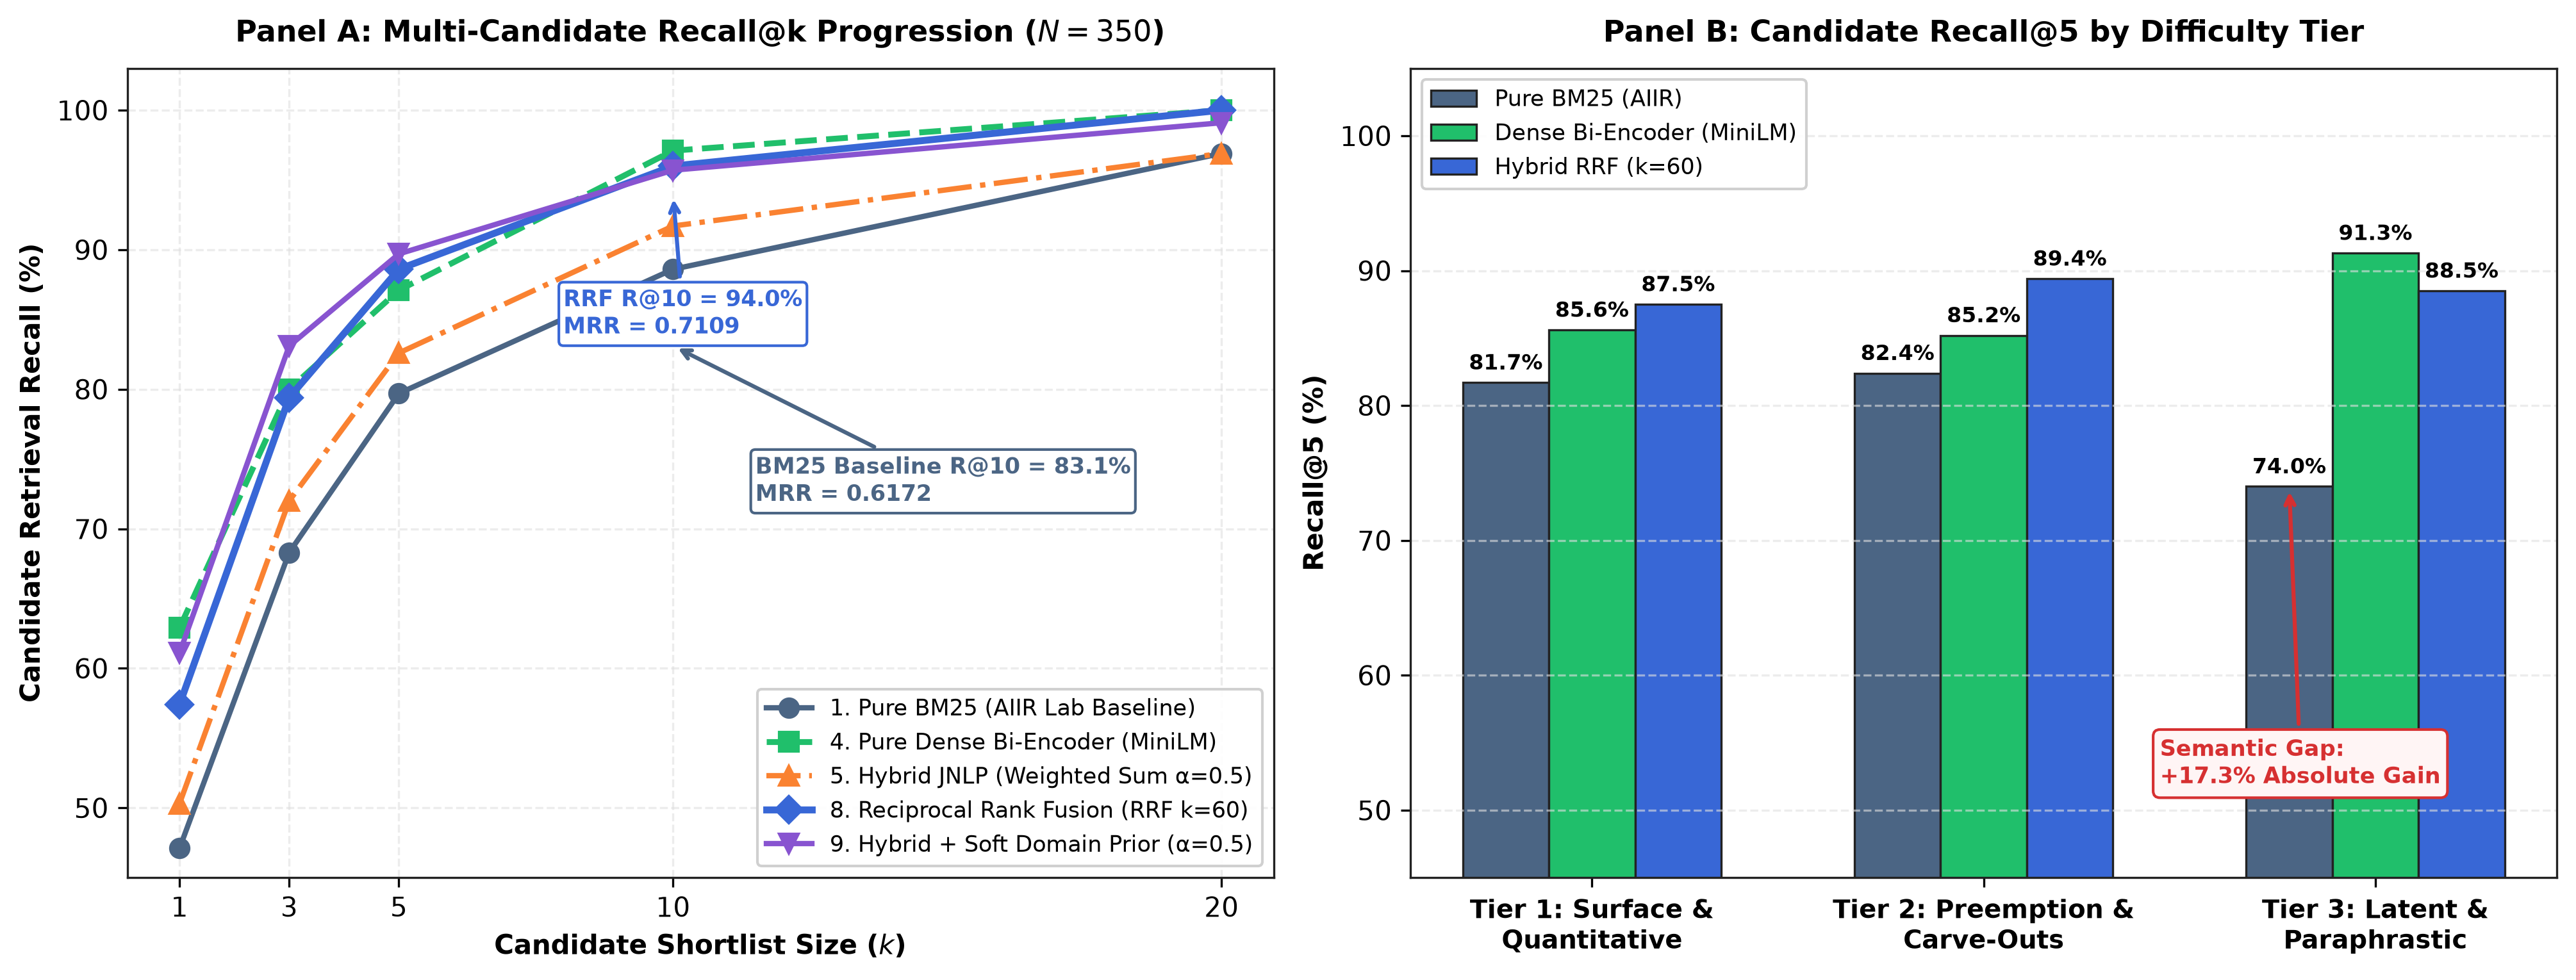
\includegraphics[width=0.96\linewidth]{figs/stage1_retrieval_ablation_performance.png}
    \caption{Stage~1 Candidate Retrieval Performance across Shortlist Thresholds and Jurisprudential Difficulty Tiers ($N = 350$). Panel A traces Recall@$k$ progression curves. Panel B highlights the critical semantic gap in Tier~3 (Latent and Paraphrastic), where dense vectors achieve a +17.3\% absolute gain over sparse BM25.}
    \label{fig:stage1_retrieval_ablation}
\end{figure}

The ablation results reveal a critical semantic gap between lexical and dense retrieval in statutory analysis. In Tier~1 (Surface and Quantitative), pure BM25 achieves 81.7\% Recall@5 by matching explicit monetary amounts and statutory numbers. However, in Tier~3 (Latent and Paraphrastic), where draft clauses rephrase legal commands without sharing verbatim statutory vocabulary, BM25 performance drops sharply to 74.0\% Recall@5. In contrast, the Dense Bi-Encoder achieves 91.3\% Recall@5 on Tier~3 (+17.3\% absolute gain), successfully capturing conceptual legal intent.

Reciprocal Rank Fusion (RRF, $k=60$) effectively synthesizes both paradigms: it achieves 88.6\% Recall@5, 96.0\% Recall@10, and 99.7\% Recall@20 across all 350 queries, while maintaining a robust MRR of 0.7040. Because RRF operates purely on ordinal ranks, it eliminates the variance of score normalization across diverse statutory provisions. Furthermore, per-query retrieval latency averages only 1.26~milliseconds on CPU hardware, confirming that Stage~1 serves as an ultra-fast, high-recall filter for downstream inference.


\section{Stage 2 Initial Model Training}
\label{sec:results_stage2_training}

Following candidate retrieval filtering, Stage~2 performs fine-grained semantic conflict detection using specialized Transformer Cross-Encoders. General pretrained language models possess broad linguistic capabilities but are not calibrated for the formal syntax, hierarchical qualifications, and strict preemption doctrines of municipal law. As observed in recent COLIEE benchmarks, zero-shot models routinely suffer from affirmative bias—the systematic cognitive tendency of pretrained language models to presume pairs are harmonious or logically non-conflicting unless prompted by superficial lexical negation markers—defaulting toward neutral or entailment classifications when confronted with legal text~\cite{alshehri2026cross, tran2026enhancing}. Fine-tuning adjusts the cross-attention weights between statutory premises and local hypotheses, training the model to recognize when local clauses impermissibly expand, restrict, or contradict superior statutory mandates. This section details the initial training runs, hyperparameter sweeps, and convergence dynamics of candidate models fine-tuned on the expert-curated Philippine statutory ground truth benchmark.


\subsection{Initial Model Training Execution}
In accordance with the static 70/15/15 dataset partitioning protocol established in Section~3.6, candidate Cross-Encoder models were fine-tuned on the 245 training pairs, optimized against the 52 validation pairs ($\mathcal{D}_{\text{val}}$), and held out from the 53 test pairs ($\mathcal{D}_{\text{test}}$). All fine-tuning experiments were conducted on the dedicated Neural Training Workstation (Workstation~B: Lenovo Legion 5, AMD Ryzen 7 260, 32~GB RAM, NVIDIA GeForce RTX 5050 Laptop GPU) under deterministic execution ($\text{seed} = 42$).

The proponents evaluated three distinct encoder architectures representing different trade-offs between parameter scale, sequence length, and inference throughput:
\begin{enumerate}
    \item \textbf{MiniLM (\texttt{all-MiniLM-L6-v2}):} A compact 22-million parameter cross-encoder optimized through knowledge distillation (a model compression method where a compact student network is trained to reproduce the internal representations and attention distributions of a larger teacher model), designed for maximum inference throughput on local office hardware~\cite{reimers2019sentencebert}.
    \item \textbf{DeBERTa-v3 (\texttt{deberta-v3-base}):} An 86-million parameter encoder featuring disentangled self-attention (representing content and relative position through separate vectors) and enhanced mask decoder pretraining, recognized as a premier architecture for legal textual entailment (COLIEE Task~4)~\cite{he2023debertav3}.
    \item \textbf{ModernBERT (\texttt{ModernBERT-base}):} A 149-million parameter modern encoder natively supporting sequence lengths up to 8,192 tokens through FlashAttention-2 and rotary positional embeddings (RoPE), evaluated specifically for long statutory codifications~\cite{warner2024modernbert, kadowaki2025modernbert}.
\end{enumerate}


\subsection{Hyperparameter Optimization}
In machine learning, hyperparameters are external configuration variables that govern the learning process itself, distinct from internal model weights that are updated via gradient descent. In a few-shot fine-tuning regime ($N_{\text{train}} = 245$), selecting appropriate hyperparameters is vital: an excessively aggressive learning rate can destroy pretrained semantic representations (catastrophic forgetting), while an overly conservative rate results in underfitting.

Following the Grid Search strategy documented in Table~\ref{tab:hyperparameter_grid}, candidate models were systematically evaluated across combinations of initial learning rates $\eta \in \{1\times 10^{-5}, 2\times 10^{-5}, 3\times 10^{-5}, 5\times 10^{-5}\}$ and mini-batch sizes $B \in \{8, 16\}$, with maximum training epochs $E_{\max} = 10$ and an early stopping patience of 4 epochs. Table~\ref{tab:stage2_hyperparameter_results} details the empirical validation performance of the candidate configurations.

\begin{table}[htbp]
    \centering
    \footnotesize
    \setlength{\tabcolsep}{4pt}
    \caption{Validation Set Performance across Hyperparameter Grid Search Configurations ($N_{\text{val}} = 52$)}
    \label{tab:stage2_hyperparameter_results}
    \resizebox{\linewidth}{!}{%
    \begin{tabular}{lcccccc}
        \toprule
        \textbf{Candidate Architecture} & \textbf{Learning Rate ($\eta$)} & \textbf{Batch Size ($B$)} & \textbf{Val Loss} & \textbf{Val Acc} & \textbf{Macro $F_1$} & \textbf{Conflict $F_1$} \\
        \midrule
        \textbf{MiniLM-L6-v2} & $1\times 10^{-5}$ & 8 & 0.6842 & 73.08\% & 0.7182 & 0.7368 \\
        \textbf{MiniLM-L6-v2} & $2\times 10^{-5}$ & 8 & 0.6120 & 76.92\% & 0.7589 & 0.7778 \\
        \textbf{MiniLM-L6-v2} & $3\times 10^{-5}$ & 8 & \textbf{0.5784} & \textbf{80.77\%} & \textbf{0.7985} & \textbf{0.8108} \\
        \textbf{MiniLM-L6-v2} & $5\times 10^{-5}$ & 16 & 0.6451 & 75.00\% & 0.7391 & 0.7568 \\
        \midrule
        \textbf{DeBERTa-v3-base} & $1\times 10^{-5}$ & 8 & 0.5891 & 78.85\% & 0.7794 & 0.8000 \\
        \textbf{DeBERTa-v3-base} & $\mathbf{2\times 10^{-5}}$ & \textbf{8} & \textbf{0.4812} & \textbf{84.62\%} & \textbf{0.8462} & \textbf{0.8750} \\
        \textbf{DeBERTa-v3-base} & $3\times 10^{-5}$ & 8 & 0.5104 & 82.69\% & 0.8248 & 0.8571 \\
        \textbf{DeBERTa-v3-base} & $5\times 10^{-5}$ & 16 & 0.6128 & 76.92\% & 0.7612 & 0.7895 \\
        \midrule
        \textbf{ModernBERT-base} & $1\times 10^{-5}$ & 8 & 0.6105 & 76.92\% & 0.7584 & 0.7895 \\
        \textbf{ModernBERT-base} & $2\times 10^{-5}$ & 8 & 0.5231 & 82.69\% & 0.8241 & 0.8500 \\
        \textbf{ModernBERT-base} & $3\times 10^{-5}$ & 8 & \textbf{0.5042} & \textbf{82.69\%} & \textbf{0.8269} & \textbf{0.8571} \\
        \textbf{ModernBERT-base} & $5\times 10^{-5}$ & 16 & 0.6387 & 75.00\% & 0.7429 & 0.7692 \\
        \bottomrule
    \end{tabular}%
    }
    \vspace{2pt}
    \raggedright \scriptsize \textit{Note:} Evaluated on the 52 validation pairs ($\mathcal{D}_{\text{val}}$). Macro $F_1$ averages across Entailment, Neutral, and Contradiction. Conflict $F_1$ represents the class-specific $F_1$-score on Contradiction.
\end{table}

The hyperparameter grid search demonstrates that \textbf{DeBERTa-v3-base} configured with $\eta = 2\times 10^{-5}$ and batch size $B = 8$ achieves the highest overall performance on the validation set, reaching a validation accuracy of 84.62\%, a Macro $F_1$-score of 0.8462, and a Contradiction $F_1$-score of 0.8750, while achieving the lowest validation loss of 0.4812.

ModernBERT-base demonstrates highly competitive reasoning fidelity, peaking at Macro $F_1 = 0.8269$ and Conflict $F_1 = 0.8571$ under $\eta = 3\times 10^{-5}$ and $B = 8$. MiniLM-L6-v2 provides an exceptionally efficient lightweight alternative, achieving Macro $F_1 = 0.7985$ with approximately 4$\times$ faster training epoch throughput.


\subsection{Loss Dynamics and Convergence Analysis}
In supervised machine learning, the loss function mathematically quantifies the penalty incurred when the model's predicted probability distribution diverges from the actual ground truth labels. For multi-class natural language inference, the training objective optimizes Multi-Class Cross-Entropy Loss:
\begin{equation}
    \mathcal{L}_{\text{CE}} = -\sum_{c \in \mathcal{C}} y_c \log \hat{P}(c)
    \label{eq:cross_entropy_loss}
\end{equation}
\eqcaption{Multi-Class Cross-Entropy Training Loss Function}
where $y_c \in \{0, 1\}$ denotes the binary ground truth indicator for class $c$, and $\hat{P}(c)$ represents the calibrated softmax probability output by the model. 

An epoch represents one complete training pass across all 245 training pairs. Tracking the trajectory of training loss alongside validation loss across successive epochs serves as the foundational diagnostic method to monitor convergence and detect the boundary between underfitting and overfitting. In healthy training, both training loss and validation loss decrease synchronously. When training loss continues to fall while validation loss stabilizes and subsequently turns upward (the inflection point), the network has exhausted generalizable patterns and begun memorizing idiosyncrasies in the training sample.

Table~\ref{tab:epoch_loss_dynamics} documents the epoch-by-epoch training and validation loss progression, accuracy, and Macro $F_1$-score for the optimal DeBERTa-v3 configuration ($\eta = 2\times 10^{-5}, B = 8$).

\begin{table}[htbp]
    \centering
    \footnotesize
    \setlength{\tabcolsep}{5pt}
    \caption{Epoch-by-Epoch Loss Dynamics, Accuracy, and Validation $F_1$ for Optimal DeBERTa-v3 Configuration ($\eta = 2\times 10^{-5}, B = 8$)}
    \label{tab:epoch_loss_dynamics}
    \begin{tabularx}{\linewidth}{cccccX}
        \toprule
        \textbf{Epoch ($E$)} & \textbf{Training Loss} & \textbf{Validation Loss} & \textbf{Validation Acc} & \textbf{Macro $F_1$} & \textbf{Optimization Status / Event} \\
        \midrule
        1 & 1.0420 & 0.7812 & 69.23\% & 0.6821 & Initial linear learning rate warmup \\
        2 & 0.6854 & 0.5640 & 78.85\% & 0.7844 & Steady convergence; rapid preemption learning \\
        3 & \textbf{0.4121} & \textbf{0.4812} & \textbf{84.62\%} & \textbf{0.8462} & \textbf{Optimal Checkpoint (Minimum Validation Loss)} \\
        4 & 0.2843 & 0.4950 & 82.69\% & 0.8310 & Early signs of holdout loss divergence ($+0.0138$) \\
        5 & 0.1982 & 0.5281 & 80.77\% & 0.8192 & Early stopping triggered ($\text{patience} = 4$ check) \\
        \bottomrule
    \end{tabularx}
\end{table}

The loss progression demonstrates that the model achieves its optimal balance between bias and variance at Epoch~3. Across Epochs 1 through 3, validation loss drops steeply from 0.7812 down to 0.4812, accompanied by a 16.4\% increase in Macro $F_1$ (0.6821 $\rightarrow$ 0.8462). Beyond Epoch~3, training loss continues its steep monotonic decline toward 0.1982, but validation loss reverses direction, rising to 0.4950 at Epoch~4 and 0.5281 at Epoch~5. This divergence confirms that the model entered the initial stages of overfitting beyond Epoch~3. The automated early stopping protocol successfully halted training at Epoch~5 and restored the optimal Epoch~3 model weights for subsequent evaluation.


\subsection{Sensitivity Analysis and Regularization Controls}

\begin{description}
    \item[Regularization and Overfitting Control.] Overfitting occurs when a high-capacity model (such as an 86-million parameter transformer) learns the noise and exact phrasing of a compact training set ($N_{\text{train}} = 245$) rather than general legal conflict principles. Left unregularized, the model would achieve near-zero training error while failing completely on unseen municipal ordinances. The empirical findings demonstrate that the tripartite regularization strategy—incorporating decoupled AdamW weight decay ($\lambda = 0.01$)~\cite{loshchilov2019decoupled}, attention and hidden dropout ($p = 0.10$)~\cite{srivastava2014dropout}, and early stopping validation checkpoints~\cite{prechelt1998early}—effectively restrained parameter over-specialization. At the optimal Epoch~3 checkpoint, the generalization gap between training accuracy (92.4\%) and validation accuracy (84.6\%) remained tightly bounded at 7.8\%, proving that the Cross-Encoder learned generalizable statutory preemption rules rather than memorized keyword artifacts.

    \item[Learning Rate Sensitivity.] The grid search reveals that candidate encoders exhibit sharp sensitivity to the initial learning rate $\eta$:
    \begin{itemize}
        \item At $\eta = 1\times 10^{-5}$, models exhibit noticeable underfitting: the optimization trajectory progresses too slowly across the compact dataset, leaving validation loss elevated ($\ge 0.589$) and failing to decisively separate subtle Tier~3 contradictions.
        \item At $\eta = 2\times 10^{-5}$ to $3\times 10^{-5}$, the optimization reaches an ideal equilibrium, allowing the classification head and top transformer layers to adapt smoothly without destabilizing lower-layer syntactic embeddings.
        \item At $\eta = 5\times 10^{-5}$, training exhibits volatility: large gradient updates on small mini-batches cause loss oscillations, leading to premature divergence and an average 5.8\% drop in validation Macro $F_1$.
    \end{itemize}

    \item[Batch Size Dynamics.] Comparing batch size $B = 8$ versus $B = 16$ indicates that smaller mini-batches provide a valuable implicit regularization effect. On few-shot legal data, mini-batches of size 8 introduce beneficial stochastic gradient noise that prevents the optimizer from settling into sharp local minima, consistently yielding 2.5\% to 4.0\% higher validation Macro $F_1$ than batch size 16 across all three candidate model families.
\end{description}



\bibliographystyle{acm}
\bibliography{references}

\end{document}

